% Template made by Diego Ceccarelli 2009 (diego.ceccarelli@gmail.com)
\documentclass[12pt, a4paper, oneside, openright, final] {book}
\usepackage[italian]{babel}
\usepackage[utf8]{inputenc}
\usepackage[T1]{fontenc}

\usepackage{graphicx}
\usepackage{fancyhdr}
\usepackage[Bjornstrup]{fncychap}
\usepackage{setspace}

\usepackage{ae,aecompl}
\usepackage{amsfonts}

\usepackage{array}
\usepackage{stmaryrd}

% aggiungo pacchetti e cose personali
%%%% Package e simili %%%%

% Migliora la gestione dei font (con PDFLaTeX)
\usepackage{microtype}

% Rientro anche nel primo capoverrso, secondo la consuetudine italiana
\usepackage{indentfirst}

% Comando \vref
\usepackage[italian]{varioref}

% vari opzioni per gli ambienti enumerate
\usepackage{enumerate}

% tabelle e didascalie
\usepackage{booktabs}
\usepackage[font=small,format=hang,labelfont={bf}]{caption}
\usepackage{subfig} % sotto-figure e sotto-tabelle

% celle multiriga nelle tabelle
\usepackage{multirow}

% Font migliori per \mathbb
\usepackage{bbm} 

% pseudo-codice
\usepackage{algorithmic} 
\usepackage{algorithm}
\floatname{algorithm}{Algoritmo}
\renewcommand{\algorithmiccomment}[1]{//#1} %commenti con //

% principalmente per l'ambiente comment
\usepackage{verbatim}

% tabelle colorate
\usepackage{colortbl}

\usepackage{array}
\usepackage{tabularx}


%%%% Teoremi e cose simili %%%%

\newtheorem{theorem}{Teorema}
\newtheorem{lemma}{Lemma}
\newtheorem{proposition}{Proposizione}
\newtheorem{corollary}{Corollario}
\newtheorem{definition}{Definizione}



%%%% Un po' di cose utili per le formule %%%%

\usepackage{mathtools}
\DeclarePairedDelimiter{\abs}{\lvert}{\rvert} %valore assoluto

% trasposta di una matrice o un vettore
\newcommand{\transpose}[1]{\ensuremath{#1^{\mathrm{T}}}} 
% vettore (in bold)
\newcommand{\vect}[1]{\ensuremath{\mathbf{#1}}}
% matrice (maiuscola in bold)
\newcommand{\matr}[1]{\ensuremath{\mathbf{\uppercase{#1}}}} 
% norma vettoriale
\DeclarePairedDelimiter{\vectnorm}{\lVert}{\rVert}
% 'e' di Nepero
\providecommand*{\eu}{\ensuremath{\mathrm{e}}}
% grafi (in bold)
\newcommand{\graph}[1]{\ensuremath{\mathbf{#1}}}
% insiemi numerici
\newcommand{\numberset}{\mathbb}
\newcommand{\N}{\numberset{N}}
\newcommand{\R}{\numberset{R}}
% definizione di insiemi
\newcommand{\setdef}[2]{\lbrace #1 \vert\ #2 \rbrace}

% forza la disposizione degli oggetti mobili al termine di una sezione
% Utile per le appendici con molte tabelle
\usepackage[section]{placeins}

% ambiente per l'introduzione dei singoli capitoli, peppe's style
\newenvironment{intro}{\sffamily}{\vspace*{2ex minus 1.5ex}}

%%%% Altro %%%%

% note a margine in rosso
\newcommand{\mnote}[1]{\marginpar{\tiny {\color{red}#1}}}

% comando TODO
\newcommand{\TODO}[1]{\begin{center}\scshape \color{red} TODO (#1)\end{center}}
\newcommand{\iTODO}[1]{\scshape \color{red} TODO (#1)} % inline TODO

%%%% Link e compagnia bella %%%%

% url e link
\usepackage{hyperref}
\hypersetup{colorlinks,
            citecolor=black,
            filecolor=black,
            linkcolor=black,
            urlcolor=black,
            pdfauthor={Giulio Visco},
			pdftitle={Modelli neurali costruttivi di tipo Reservoir Computing per domini strutturati}
}
\usepackage{bookmark}
\usepackage{url}

\newenvironment{abstract}%
{\cleardoublepage\null\vfill\begin{center}%
\bfseries\abstractname\end{center}}%
{\vfill\null}
\setlength{\headheight}{15pt}


\newenvironment{grazie}%
{\cleardoublepage\null\vfill\begin{center}%
\bfseries Ringraziamenti \end{center}}%
{\vfill\null}
\setlength{\headheight}{15pt}


\begin{document}

%interlinea a 1.5
%\onehalfspacing
\doublespacing
%\linespread{1.3}

\frontmatter
 
%\pdfbookmark{Title}{Title}
\begin{titlepage}
\begin{center}

\begin{large}\textbf{\sc Università di Pisa}\end{large}

%\vspace{0.2cm}
\vspace{0.4cm}

%
\includegraphics[scale=0.3]{img/cherubino}

\includegraphics[width=0.5\columnwidth]{img/cherubino}

%\vspace{0.4cm}

\begin{large}
\sc Facolt\`a di Scienze Matematiche, Fisiche e Naturali \\
Corso di Laurea Specialistica in Informatica
\end{large}

\vspace{1.0cm}

\begin{large}
Tesi di laurea
\end{large}

% \vspace{1.6cm}
\vspace{0.4cm}


{\Huge \bfseries \Large Modelli neurali costruttivi di tipo Reservoir Computing per domini strutturati}%\\[1.0cm]


\vspace{0.4cm}

\begin{large}
Giulio Visco
\end{large}

\vspace{0.7cm}

\begin{large}
\begin{tabular*}{0.9\textwidth}{c @{\extracolsep{\fill}} c}
Relatori	  &  Controrelatore\\
Prof. Alessio Micheli & Prof. Stefano Chessa \\
Dott. Claudio Gallicchio & \\
\end{tabular*}
\end{large}

% \vspace{1.6cm}
%\vspace{0.5cm}
\vspace*{\stretch{1.0}} 

Anno Accademico 2010/2011

\end{center}
\end{titlepage}


\thispagestyle{empty}
\cleardoublepage
% \thispagestyle{empty}
% \vspace*{\stretch{1}}
% \begin{flushright}
% \em gfsdkojfids fkdhffd\\
% gfgf
% \end{flushright}
%  \vspace*{\stretch{3}} \clearpage
% 
% \thispagestyle{empty}
% \cleardoublepage



% dedica
\begin{flushright}
In God we trust, all others bring data.\\
     --- William Edwards Deming
\end{flushright}



\newpage
\begin{abstract}
Il presente lavoro di tesi introduce e discute nuovi modelli di Reti Neurali Ricorsive per l'apprendimento supervisionato di trasduzioni su grafi. Due sono i maggiori contributi apportati: l'adozione di un approccio costruttivo, e l'introduzione di un meccanismo stabile di output-feedback, entrambi innovativi nell'ambito del Reservoir Computing a cui si rifanno i modelli considerati. La combinazione di una strategia costruttiva e dell'utilizzo di modelli di Reservoir Computing ha inoltre permesso la realizzazione di modelli molto efficienti dal punto di vista computazionale.

I modelli e le strategie individuate si configurano come uno strumento utile e flessibile nel trattamento di domini complessi attraverso tecniche di Machine Learning, e propongono soluzioni ad alcuni dei problemi aperti nell'ambito del Reservoir Computing.

L'analisi sperimentale svolta riguarda l'apprendimento di trasduzioni strutturali da dataset reali appartenenti all'ambito della Chemioinformatica.



\begin{comment}
\small
Il Machine Learning si propone di ampliare la classe dei problemi trattabili laddove non risultino applicabili approcci algoritmici o analitici. Rilevante è dunque in questo ambito il trattamento di domini strutturati: poiché in numerosi campi le relazioni tra i dati possono essere rappresentate sotto forma di grafi, estendere la gamma di strategie utili ad apprendere trasduzioni strutturali può infatti dare risposta a problemi esistenti e permettere lo sviluppo di nuove applicazioni.

Nel contesto del Machine Learning, il trattamento di domini strutturati attraverso il paradigma neurale trova principalmente due ostacoli: l'alto costo computazionale e la presenza di vincoli sulla classe degli input trattabili. Il Reservoir Computing propone soluzioni ad entrambi i problemi, offrendo modelli efficienti in grado di apprendere trasduzioni strutturali definite su grafi generici. 

Nel corso della tesi vengono introdotti nuovi modelli di Reti Neurali Ricorsive, nell'ambito del Reservoir Computing, per l'apprendimento supervisionato di trasduzioni su grafi. I modelli proposti si caratterizzano per l'adozione di un approccio costruttivo, innovativo nell'ambito del Reservoir Computing, che permette di individuare soluzioni ad alcuni dei problemi che caratterizzano i modelli esistenti. I modelli proposti permettono infatti la determinazione della topologia della rete attraverso un processo adattivo e la realizzazione di un meccanismo stabile di output-feedback per introdurre informazione supervisionata all'interno del processo di encoding del reservoir. La strategia costruttiva permette inoltre la realizzazione di modelli molto efficienti dal punto di vista computazionale.

L'analisi sperimentale svolta riguarda l'apprendimento di trasduzioni strutturali da dataset reali appartenenti all'ambito della Chemioinformatica.
\end{comment}
\end{abstract}
\newpage
\pagestyle{plain}

%ringraziamenti
\begin{grazie}
Il mio primo ringraziamento va al professor Alessio Micheli, per avermi introdotto al mondo del Machine Learning e per avermi coinvolto in un'esperienza didattica diversa e stimolante, fatta di idee e di discussioni, di ricerche e di ricerca. Conserverò un ricordo prezioso delle lezioni, delle riunioni, dei consigli e delle piacevoli chiacchierate.

Un ringraziamento particolare va anche a Claudio Gallicchio che mi ha guidato in questo lungo e non sempre facile percorso, tendendomi la mano o pungolandomi secondo necessità. Tutto quello che segue è anche merito suo, e chissà se troverò mai il modo di ripagarlo del supporto ricevuto --- tecnico e soprattutto umano --- o anche solo di farmi perdonare dei grattacapi che ha dovuto subire per vedermi arrivare in fondo a questa tesi.

Ci sarebbero altre persone da ringraziare, e non sarebbero poche: amici vicini e lontani, recenti o di vecchia data, parenti, coinquilini e case, qualche professore, qualche luogo. A molti devo un ringraziamento per i consigli, per avermi supportato o semplicemente distratto, per aver ascoltato le mie lamentele o per aver cercato di capire cosa stessi combinando. Sono troppi perché un elenco possa rendere giustizia a tutti: nessuno se ne abbia a male dunque se qui sorvolo, nella speranza di poter ringraziare ognuno come merita.

Ogni singola parola, formula, tabella o figura di questa tesi è dedicata a mia madre e Cecilia, che mi hanno supportato e sopportato più di quanto si potesse desiderare.
\end{grazie}


\tableofcontents % indice
\listoffigures % lista delle figure
\listoftables % lista delle tabelle
 
% header per l'introduzione
\newpage
\pagestyle{fancy}
 \renewcommand{\chaptermark}[1]{
  \markboth{#1}{}}
 \renewcommand{\sectionmark}[1]{}

\chapter{Introduzione}
Il Machine Learning \cite{Mitchell:ML, Hastie:EOSL} si propone di ampliare la classe dei problemi trattabili laddove non risultino applicabili approcci algoritmici o analitici. Rilevante è in questo ambito il trattamento di domini strutturati: in molti settori applicativi, infatti, i dati trattati trovano una propria rappresentazione naturale in forma di grafi. Estendere le metodologie di Machine Learning per affrontare problemi definiti su domini strutturati rappresenta dunque un'opportunità per dare risposte efficaci a problemi esistenti, aprendo spazio per lo sviluppo di nuove applicazioni.

Nel realizzare questo obiettivo, quanto verrà discusso nel seguito si orienta in particolare al paradigma neurale, che nell'ambito del Machine Learning ricopre un ruolo rilevante, attingendo a tecniche e modelli esistenti per introdurre soluzioni originali nel campo del trattamento dei domini strutturati. Le Reti Neurali Artificiali \cite{Haykin:NN,Bishop:NNFPR} sono infatti un insieme vasto e variegato di modelli computazionali, efficacemente applicati a problemi reali. Nate per sfruttare un approccio connessionista di rappresentazione delle informazioni, le Reti Neurali Artificiali offrono importanti caratteristiche computazionali e, nella loro forma più semplice di Reti Neurali Feedforward \cite{Bishop:NNFPR,Haykin:NN}, risultano in grado di approssimare con precisione arbitraria qualsiasi funzione continua~\cite{Cybenko:ApproximationBySuperpositions}.

Benché l'apprendimento in una Rete Neurale Artificiale avvenga modificando i pesi sulle connessioni, nascono nell'ambito delle Reti Neurali Feedforward anche algoritmi e strategie che guardano alla struttura della rete e alla sua realizzazione per migliorarne o semplificarne il processo di creazione e di allenamento. L'approccio costruttivo \cite{Smieja:NeuralNetworkConstructive,Fahlman:CC,Littmann:learningAndGeneralization}, ad esempio, propone un procedimento incrementale per la costruzione della rete nella suo complesso, secondo un meccanismo guidato direttamente dalle caratteristiche del problema affrontato. 
In questo caso la rete cresce in maniera iterativa, potendo sfruttare ad ogni passo tutte le informazioni precedentemente apprese ed adattando la propria dimensione alla complessità del problema. Ne risulta il vantaggio di non dover stabilire a priori la topologia della rete, strettamente legata alla sua capacità computazionale, e di poter scomporre il problema in sotto-problemi, singolarmente affrontati attraverso procedimenti di allenamento più semplici e computazionalmente efficienti.

Nonostante le Reti Neurali Feedforward, usate per apprendere funzioni definite su vettori, siano la classe di Reti Neurali Artificiali più ampiamente diffusa nel contesto dei Machine Learning, l'approccio neurale propone anche paradigmi e modelli orientati all'apprendimento su domini più complessi.
\`E il caso delle Reti Neurali Ricorrenti \cite{Tsoi:DiscreteTimeRNN, Elman:FindingStructure}, che generalizzano le Reti Neurali Feedforward al trattamento di sequenze attraverso l'introduzione di cicli nella topologia delle connessioni fra le unità.
Benché reti di questo tipo risultino efficienti nel contesto del Machine Learning, il costo computazionale del loro allenamento risulta un campo di studio aperto; è in questo contesto infatti che nasce il paradigma del Reservoir Computing \cite{Lukosevicius:ESN-Survey,Verstraeten:AnExperimentalUnification,Jaeger:HarnessingNonlinearity}: una classe di modelli caratterizzati dalla separazione concettuale tra una parte ricorrente (i.e. con connessioni cicliche fra le unità) ed una parte non-ricorrente per il calcolo del segnale di uscita. 
L'opportunità di limitare l'apprendimento alla sola parte non-ricorrente del modello, lasciando inalterata la parte ricorrente, rappresenta il punto di forza del Reservoir Computing, consentendo l'impiego di strategie di allenamento molto efficienti dal punto di vista computazionale. A fronte di questo vantaggio la presenza di una porzione di rete non soggetta ad allenamento determina un limite per i modelli esistenti: una parte delle dinamiche della rete risulta infatti fissata a priori e non ha la capacità di adattarsi al problema affrontato.

L'apprendimento di funzioni definite su domini strutturati (i.e. trasduzioni strutturali), obiettivo della tesi, è affrontato in ambito neurale attraverso le Reti Neurali Ricorsive \cite{Frasconi:AGeneralFramework, Sperduti:SupervisedNeuralNetworks}, che generalizzano le Reti Neurali Ricorrenti. 
Benché in svariati campi si abbiano esempi applicativi di modelli neurali ricorsivi --- per citarne solo alcuni, nella Chimica \cite{Bianucci:ApplicationOfCascade,Micheli:AnalysisOfTheInternal,Bertinetto:EvaluationOfHierarchical}, nella Proteomica \cite{Baldi:ThePrincipledDesign}, nel trattamento e riconoscimento di immagini \cite{Frasconi:AGeneralFramework} o nell'Ingegneria del Software \cite{Frasconi:AGeneralFramework} --- il legame fra la topologia dell'input e le dinamiche interne della rete impone, nelle Reti Neurali Ricorsive, dei vincoli sulla classe degli input trattabili: nella loro formulazione originale, reti di questo tipo risultano infatti applicabili unicamente a dati strutturati che presentino un ordinamento topologico fra i vertici, il che limita il dominio di input alla sola classe dei Grafi Diretti Aciclici. Tale assunzione ha impatto sulla capacità dei modelli \cite{Micheli:ContextualProcessing}, limitando dunque il numero di problemi affrontabili rispetto a quanto avverrebbe potendo trattare la classe più generale dei grafi.
\\
In risposta a questa esigenza, nella storia recente delle Reti Neurali Ricorsive si ritrovano vari modelli tesi all'ampliamento della classe di input. Due approcci distinti, in particolare, lasciano emergere elementi interessanti per la realizzazione di modelli neurali in grado di apprendere trasduzioni strutturali definite su grafi.\\
Il modello \emph{Neural Networks for Graphs} (NN4G) \cite{Micheli:NN4G} adotta una strategia costruttiva per evitare i problemi determinati dalla presenza di cicli nell'input e per sfruttare localmente informazioni globali, legate alla topologia dei dati: ad ogni iterazione del processo di costruzione della rete, infatti, nuove informazioni relative alla struttura del grafo vengono raccolte e rese disponibili per semplificare l'apprendimento nelle unità aggiunte successivamente.\\
Un approccio differente è individuato dal modello \emph{Graph Echo State Network} (GraphESN) \cite{Gallicchio:GraphESN}, appartenente all'ambito del Reservoir Computing, che sfrutta le caratteristiche strutturali della rete per realizzare il trattamento di domini strutturati generici. Ne risulta un modello di Rete Neurale Ricorsiva efficiente per l'apprendimento di trasduzioni strutturali definite su grafi, che tuttavia mantiene inalterate alcune delle criticità caratteristiche del Reservoir Computing.

Da quanto detto emergono dunque necessità e limitazioni legate all'apprendimento su domini strutturati attraverso il paradigma neurale.
In particolare, in una disciplina fortemente orientata alle applicazioni come il Machine Learning, il costo computazionale e la classe degli input trattabili risultano essere aspetti molto rilevanti. Il paradigma del Reservoir Computing offre strumenti efficaci per rispondere a simili necessità, ma presenta tuttavia degli elementi critici, legati alla presenza di una porzione di rete fissata a priori e mantenuta inalterata durante l'apprendimento. La determinazione della topologia appropriata e l'opportunità di modificare le dinamiche dell'intera rete sulla base del problema affrontato, sono infatti limiti la cui risoluzione rimane ad oggi un problema aperto \cite{Lukosevicius:ESNwithTrainedFeedbacks,Wyffels:stableOutputFeedback,Reinhart:ReservoirRegularization}.
L'approccio costruttivo offre soluzioni in tal senso, proponendo una strategia efficiente per determinare la struttura della rete in maniera automatica e per sfruttare le informazioni raccolte nel corso del processo incrementale di costruzione della rete.
\\
Quanto discusso nel seguito ha dunque l'obiettivo di sintetizzare questi elementi, introducendo nuovi modelli ricorsivi appartenenti all'ambito del Reservoir Computing, che permettano l'adozione di una strategia costruttiva nell'apprendimento di trasduzioni strutturali.
In particolare, i modelli descritti nel seguito rappresentano un'estensione delle GraphESN, caratterizzandosi dunque come modelli efficienti per il trattamento di domini strutturati generali. L'introduzione della strategia costruttiva, innovativa nell'ambito del Reservoir Computing, ha impatto sui modelli proposti dal punto di vista computazionale ed algoritmico, riducendo il costo necessario all'allenamento ed evitando il problema di dover fissare a priori la topologia della rete. L'opportunità di sfruttare localmente informazioni globali e supervisionate viene invece usata per modificare le dinamiche di quella porzione di rete che nel Reservoir Computing non è soggetta ad allenamento. Ne risulta un meccanismo stabile per introdurre informazione supervisionata, anche in assenza di una fase di adattamento specifica, che possa influenzare le dinamiche della rete in maniera consistente con il problema affrontato.

Le capacità dei modelli introdotti sono testate, attraverso una procedura rigorosa di validazione, su problemi di Chemioinformatica relativi a dataset reali noti in letteratura. Parte dei risultati riportati nel seguito è inoltre oggetto dell'articolo \textit{Constructive Reservoir Computation with Output Feedbacks for Structured Domains} \cite{Gallicchio:ConstructiveReservoir}, che sarà discusso nel corso del XX European Symposium on Artificial Neural Networks, Computational Intelligence and Machine Learning\footnote{\url{http://www.dice.ucl.ac.be/esann/}}.

% contenuti
L'esposizione degli argomenti nel testo è articolata come segue:
\begin{description}
\item[Nel capitolo~\ref{ch:background}] si introducono i temi, le tecniche ed i modelli alla base del lavoro svolto. Nel corso di questa rassegna dello stato dell'arte vengono in particolare presentati i principi dell'approccio costruttivo e del Reservoir Computing, descrivendo anche modalità ed obiettivi nel trattamento dei domini strutturati.
\item[Nel capitolo~\ref{ch:modelli}] vengono introdotti i modelli originali, oggetto del lavoro di tesi, ne vengono presentate le caratteristiche e discussi gli aspetti specifici.
\item[Nel capitolo~\ref{ch:esperimenti}] sono descritti i risultati sperimentali ottenuti testando le capacità dei modelli su una serie di problemi del mondo reale appartenenti all'ambito della Chemioinformatica. 
\item[Nel capitolo~\ref{ch:conclusioni}] viene presentata una valutazione del lavoro svolto, con l'obiettivo di determinare vantaggi e criticità dei modelli proposti nonché di individuare di quegli aspetti che potrebbero essere oggetto di un ulteriore, specifico, lavoro di indagine e sperimentazione.
\end{description}

%\begin{comment}
%
%% Estensione delle metodologie per trattare domini strutturati e Machine Learning
%Il Machine Learning \cite{Mitchell:ML, Hastie:EOSL} si propone di ampliare la classe dei problemi trattabili laddove non risultino applicabili approcci algoritmici o analitici. Rilevante è dunque in questo ambito il trattamento di domini strutturati: in molti settori applicativi, infatti, i dati trattati trovano una propria rappresentazione naturale in forma di grafi. Per citarne solo alcuni, si hanno esempi in questo senso nella Chimica \cite{Bianucci:ApplicationOfCascade,Micheli:AnalysisOfTheInternal,Bertinetto:EvaluationOfHierarchical}, nella Proteomica \cite{Baldi:ThePrincipledDesign}, nel trattamento e riconoscimento di immagini \cite{Frasconi:AGeneralFramework} o nell'Ingegneria del Software \cite{Frasconi:AGeneralFramework}. Estendere le metodologie di Machine Learning per affrontare problemi definiti su domini strutturati, rappresenta quindi un modo per dare risposte efficaci a problemi esistenti, aprendo spazio per lo sviluppo di nuove applicazioni.
%
%% Approccio neurale: Reti Neurali Artificiali
%Nell'ambito del Machine Learning il paradigma neurale ricopre un ruolo rilevante. Le Reti Neurali Artificiali \cite{Haykin:NN,Bishop:NNFPR} sono infatti un insieme vasto e variegato di modelli computazionali, efficacemente applicati a problemi reali. In analogia con il modello biologico, in una Rete Neurale Artificiale numerose unità (neuroni) sono collegate fra loro attraverso connessioni pesate (sinapsi) che permettono ad un segnale (attivazione) di propagarsi. 
%La configurazione della topologia e dei pesi sulle connessioni ha dunque impatto sul modo in cui il segnale di ingresso viene propagato, e quindi sul segnale di uscita. Grazie a questo, le Reti Neurali Feedforward \cite{Bishop:NNFPR,Haykin:NN}, caratterizzate dal susseguirsi di più livelli di unità non lineari connesse fra loro secondo una topologia aciclica, risultano essere approssimatori universali \cite{Cybenko:ApproximationBySuperpositions} e sono in grado cioè di approssimare con precisione arbitraria qualsiasi funzione continua.
%%L'apprendimento supervisionato in una Rete Neurale Artificiale avviene dunque adattando i pesi delle connessioni con il fine di approssimare una funzione non nota, a partire da dati di esempio. 
%
%% Approccio costruttivo
%
%Benché l'apprendimento in una Rete Neurale Artificiale avvenga modificando i pesi sulle connessioni, nascono nell'ambito delle Reti Neurali Feedforward anche algoritmi e strategie che guardano alla struttura della rete per migliorarne o semplificarne il processo di creazione e di allenamento. L'approccio costruttivo \cite{Smieja:NeuralNetworkConstructive,Fahlman:CC,Littmann:learningAndGeneralization}, ad esempio, propone un procedimento incrementale per la costruzione della rete nel suo complesso: iterativamente singole unità vengono aggiunte, collegate alle precedenti ed allenate, secondo un meccanismo guidato dalle caratteristiche del problema affrontato. La rete, dunque, cresce in maniera incrementale, sfruttando ad ogni iterazione tutte le informazioni precedentemente apprese.
%%Facendo leva sull'importanza che la topologia delle connessioni ricopre nel determinare le caratteristiche di una rete, nasce nel contesto delle Reti Neurali Feedforward l'idea di adottare un approccio costruttivo \cite{Smieja:NeuralNetworkConstructive,Fahlman:CC,Littmann:learningAndGeneralization}
%%L'idea di adottare un approccio costruttivo \cite{Smieja:NeuralNetworkConstructive,Fahlman:CC,Littmann:learningAndGeneralization} nasce nel contesto delle Reti Neurali Feedforward con lo scopo di semplificare il processo di creazione e di allenamento dei modelli. La strategia proposta in questo caso sfrutta infatti un procedimento incrementale per la costruzione della rete nella sua totalità: iterativamente singole unità vengono aggiunte alla rete, collegate alle precedenti ed allenate, secondo un meccanismo guidato dalle caratteristiche del problema affrontato. La rete, dunque, cresce in maniera incrementale, sfruttando ad ogni iterazione tutte le informazioni precedentemente apprese.\\
%L'adozione dell'approccio costruttivo offre il vantaggio di non dover stabilire a priori la topologia della rete, strettamente legata alla sua capacità computazionale, riducendo inoltre il costo computazionale dell'allenamento, che in questo caso risulta circoscritto a singole unità e può dunque essere svolto tramite algoritmi più semplici ed efficienti. 
%Da un punto di vista più generale, la strategia costruttiva evidenzia inoltre come il paradigma neurale offra naturalmente gli strumenti necessari alla suddivisione di un problema in sotto-problemi, che si rispecchia nella visione concettuale di una rete come formata da più parti che cooperano fra loro.
%
%% Reti Neurali Ricorrenti e Reservoir Computing
%Nonostante le Reti Neurali Feedforward, usate per apprendere funzioni definite su vettori, siano la classe di Reti Neurali Artificiali più ampiamente diffusa nel contesto dei Machine Learning, l'approccio neurale propone anche paradigmi e modelli orientati all'apprendimento su domini più complessi.
%%Ampiamente diffuso per l'apprendimento di funzioni definite su vettori, l'approccio neurale propone anche paradigmi e modelli orientati all'apprendimento su domini più complessi.
%%Benché sia stato a lungo legato all'apprendimento di funzioni definite su vettori, l'approccio neurale ha visto nascere paradigmi e modelli orientati all'apprendimento su domini più complessi. 
%\`E il caso delle Reti Neurali Ricorrenti \cite{Tsoi:DiscreteTimeRNN, Elman:FindingStructure}, che generalizzano le Reti Neurali Feedforward al trattamento di sequenze, attraverso l'introduzione di cicli nella topologia delle connessioni fra le unità.\\
%Benché reti di questo tipo risultino efficienti nell'ambito del Machine Learning per domini strutturati, il costo computazionale del loro allenamento risulta un campo di studio aperto.
%\`E in questo contesto infatti che nasce il paradigma del Reservoir Computing \cite{Lukosevicius:ESN-Survey,Verstraeten:AnExperimentalUnification,Jaeger:HarnessingNonlinearity}: una classe di modelli caratterizzati dalla separazione concettuale tra una parte ricorrente (i.e. con connessioni cicliche fra le unità) ed una parte non-ricorrente per il calcolo del segnale di uscita. 
%L'opportunità di limitare l'apprendimento alla sola parte non-ricorrente del modello, lasciando inalterata la parte ricorrente, rappresenta il punto di forza dell'approccio individuato dal Reservoir Computing, consentendo l'impiego di strategie di allenamento molto efficienti dal punto di vista computazionale. A fronte di questo vantaggio, tuttavia, la presenza di dinamiche di stato che non vengono interessate da alcun tipo di adattamento rappresenta un limite per i modelli esistenti di Reservoir Computing: una parte delle dinamiche della rete risulta infatti fissata a priori e non ha la capacità di adattarsi al problema affrontato.
%
%% Reti Neurali Ricorsive 
%L'obiettivo dell'apprendimento di funzioni definite su domini strutturati (i.e. trasduzioni strutturali) è affrontato, in ambito neurale, attraverso le Reti Neurali Ricorsive \cite{Frasconi:AGeneralFramework, Sperduti:SupervisedNeuralNetworks}, che generalizzano le Reti Neurali Ricorrenti.
%Il legame fra la topologia dell'input e le dinamiche interne della rete impone tuttavia in questo caso dei vincoli sulla classe degli input trattabili. Nella loro formulazione originale, infatti, le Reti Neurali Ricorsive risultano applicabili unicamente a dati strutturati che presentino un ordinamento topologico fra i vertici, il che limita il dominio di input ai soli Grafi Diretti Aciclici. Tale assunzione ha impatto sulla capacità dei modelli \cite{Micheli:ContextualProcessing}, limitando il numero di problemi efficacemente affrontabili rispetto a quanto avverrebbe potendo trattare la classe più generale dei grafi.
%
%% NN4G e GraphESN
%Nella storia recente delle Reti Neurali Ricorsive si ritrovano vari modelli tesi all'ampliamento della classe degli input trattabili, orientati dunque all'apprendimento di trasduzioni strutturali generiche. 
%Due approcci distinti, in particolare, lasciano emergere elementi interessanti per la realizzazione di modelli neurali in grado di trattare domini strutturati generici (i.e. grafi).\\
%Il modello \emph{Neural Networks for Graphs} (NN4G) \cite{Micheli:NN4G} sfrutta un approccio costruttivo per evitare i problemi legati alla presenza di cicli nell'input. L'adozione di una strategia costruttiva permette inoltre in questo caso di sfruttare localmente informazioni globali, legate alla topologia dell'input. Ad ogni ciclo del processo di costruzione della rete, infatti, nuove informazioni relative alla struttura dei dati vengono raccolte e rese disponibili per le unità aggiunte successivamente.\\
%Un secondo esempio di Reti Neurali Ricorsive per il trattamento di grafi è dato dal modello \emph{Graph Echo State Network} (GraphESN) \cite{Gallicchio:GraphESN}, appartenente all'ambito del Reservoir Computing, che sfrutta le caratteristiche strutturali della rete per realizzare il trattamento di domini strutturati generici. Ne risulta dunque un modello di Rete Neurale Ricorsiva efficiente per l'apprendimento di trasduzioni strutturali definite su grafi, che tuttavia mantiene inalterate alcune delle criticità caratteristiche del Reservoir Computing.
%
%
%% Motivazioni e limitazioni
%Da quanto detto emergono dunque necessità e limitazioni legate all'apprendimento di trasduzioni strutturali attraverso il paradigma neurale.
%In una disciplina fortemente orientata alle applicazioni come il Machine Learning, il costo computazionale e la classe degli input trattabili rappresentano infatti degli aspetti molto rilevanti. Il paradigma del Reservoir Computing offre soluzioni efficaci per rispondere a simili necessità, ma presenta tuttavia degli elementi critici. In particolare la presenza di una porzione di rete fissata a priori, e mantenuta inalterata durante l'apprendimento, si configura come una limitazione. La determinazione della topologia di rete appropriata e l'opportunità di modificare le dinamiche dell'intera rete sulla base del problema affrontato, sono infatti limiti la cui risoluzione rimane ad oggi un problema aperto \cite{Lukosevicius:ESNwithTrainedFeedbacks,Wyffels:stableOutputFeedback,Reinhart:ReservoirRegularization}.
%L'approccio costruttivo offre tuttavia soluzioni in tal senso, proponendo una strategia efficiente per determinare la topologia della rete in maniera automatica e per sfruttare le informazioni raccolte nel corso del processo incrementale di costruzione della rete.
%
%
%% Cosa ci proponiamo di fare
%Quanto verrà discusso nel seguito ha dunque l'obiettivo di introdurre nuovi modelli di Reti Neurali Ricorsive appartenenti all'ambito del Reservoir Computing, che permettano l'adozione di una strategia costruttiva nell'apprendimento di trasduzioni strutturali. In particolare, i modelli descritti nel seguito rappresentano un'estensione delle GraphESN, caratterizzandosi dunque come modelli efficienti per il trattamento di domini strutturati generali. L'introduzione della strategia costruttiva, innovativa nell'ambito del Reservoir Computing, ha impatto sui modelli proposti dal punto di vista computazionale ed algoritmico, riducendo il costo computazionale ed evitando il problema di dover fissare a priori la topologia della rete. Applicato al trattamento dei domini strutturati, inoltre, l'approccio costruttivo offre l'opportunità di sfruttare localmente informazioni globali e supervisionate. Tale caratteristica viene usata, nei modelli proposti, per influenzare le dinamiche di quella porzione di rete che nel Reservoir Computing non è soggetta ad allenamento. Ne risulta un meccanismo stabile per introdurre informazione supervisionata, anche in assenza di una fase di adattamento specifica, che possa influenzare le dinamiche della rete in maniera consistente con il problema affrontato.
%
%Le capacità dei modelli introdotti sono testate, attraverso una procedura rigorosa di validazione, su problemi di Chemioinformatica relativi a dataset reali noti in letteratura. Parte dei risultati riportati nel seguito è inoltre oggetto dell'articolo \textit{Constructive Reservoir Computation with Output Feedbacks for Structured Domains} \cite{Gallicchio:ConstructiveReservoir}, che sarà discusso nel corso del XX European Symposium on Artificial Neural Networks, Computational Intelligence and Machine Learning\footnote{\url{http://www.dice.ucl.ac.be/esann/}}.
%
%% contenuti
%L'esposizione degli argomenti nel testo è articolata come segue:
%\begin{description}
%\item[Nel capitolo~\ref{ch:background}] si introducono i temi, le tecniche ed i modelli alla base del lavoro svolto. Nel corso di questa rassegna dello stato dell'arte vengono in particolare presentati i principi dell'approccio costruttivo e del Reservoir Computing, descrivendo anche modalità ed obiettivi nel trattamento dei domini strutturati.
%\item[Nel capitolo~\ref{ch:modelli}] vengono introdotti i modelli originali, oggetto del lavoro di tesi, ne vengono presentate le caratteristiche e discussi gli aspetti specifici.
%\item[Nel capitolo~\ref{ch:esperimenti}] sono descritti i risultati sperimentali ottenuti testando le capacità dei modelli su una serie di problemi del mondo reale appartenenti all'ambito della Chemioinformatica. 
%\item[Nel capitolo~\ref{ch:conclusioni}] la tesi si conclude con una valutazione del lavoro svolto nonché l'individuazione di quegli aspetti che potrebbero essere oggetto di un ulteriore, specifico, lavoro di indagine e sperimentazione.
%\end{description}
%
%
%\end{comment}


%%%%%%%%%%%%%%%%%%%%%%%%%%%%%%%%%%%%%%%%%%%%%%%%%%%%%%%%%%%%%%%%%%%
%%%%%%%%%%%%%%%%%%%%%%%%%%%%%%%%%%%%%%%%%%%%%%%%%%%%%%%%%%%%%%%%%%%
%%%%%%%%%%%%%%%%%%%%%%%%%%%%%%%%%%%%%%%%%%%%%%%%%%%%%%%%%%%%%%%%%%%
%%%%%%%%%%%%%%%%%%%%%%%%%%%%%%%%%%%%%%%%%%%%%%%%%%%%%%%%%%%%%%%%%%%

%\begin{comment}
%Il Machine Learning \cite{Mitchell:ML, Hastie:EOSL} si propone di ampliare la classe dei problemi trattabili laddove non risultino applicabili approcci algoritmici o analitici. Rilevante è dunque in questo ambito il trattamento di domini strutturati: in molti settori applicativi, infatti, i dati trattati trovano una propria rappresentazione naturale in forma di grafi. Estendere le metodologie di Machine Learning per affrontare problemi definiti su domini strutturati, rappresenta quindi un modo per dare risposte efficaci a problemi esistenti, aprendo spazio per lo sviluppo di nuove applicazioni. Spostare la frontiera che delimita i problemi trattabili è dunque l'obiettivo di fondo della tesi, affrontato proponendo nuovi modelli di Machine Learning che possano apprendere funzioni definite su grafi.
%
%Dei vari approcci possibili nel contesto del Machine Learnig, i modelli realizzati si rifanno a quello neurale. Le Reti Neurali Artificiali \cite{Haykin:NN,Bishop:NNFPR} sono infatti un insieme vasto e variegato di modelli computazionali che trovano impiego in numerosi contesti applicativi e che, benché siano ampiamente diffuse per l'apprendimento di funzioni definite su vettori, offrono strumenti utili al trattamento di domini complessi. 
%Attraverso le Reti Neurali Ricorrenti \cite{Tsoi:DiscreteTimeRNN, Elman:FindingStructure} è infatti possibile apprendere delle trasduzioni di sequenza, ovvero delle funzioni definite su un dominio di sequenze temporali, mentre le Reti Neurali Ricorsive \cite{Frasconi:AGeneralFramework, Sperduti:SupervisedNeuralNetworks} realizzano l'apprendimento su domini strutturati. Grazie a queste classi di modelli, il paradigma neurale ha subito una notevole evoluzione negli ultimi anni, rivelandosi efficace nel trattamento di numerosi problemi reali. 
%
%Le Reti Neurali Ricorrenti \cite{Tsoi:DiscreteTimeRNN, Elman:FindingStructure} e le Reti Neurali Ricorsive \cite{Frasconi:AGeneralFramework, Sperduti:SupervisedNeuralNetworks} permettono infatti, rispettivamente, di apprendere funzioni definite 
%
%Le Reti Neurali Artificiali \cite{Haykin:NN,Bishop:NNFPR}, in larga parte applicate per l'apprendimento di funzioni definite su vettori, offrono infatti modelli e tecniche per il 
%
%Quello delle Reti Neurali Artificiali \cite{Haykin:NN,Bishop:NNFPR} è un paradigma rilevante nell'ambito del Machine Learning
%Dei vari approcci possibili nel contesto del Machine Learning per il trattamento di domini strutturati, quello neurale ha subito una notevole evoluzione negli ultimi anni, rivelandosi efficace nel trattamento di numerosi problemi reali. Per citarne solo alcuni, si hanno esempi in questo senso nella Chimica \cite{Bianucci:ApplicationOfCascade,Micheli:AnalysisOfTheInternal,Bertinetto:EvaluationOfHierarchical}, nella Proteomica \cite{Baldi:ThePrincipledDesign}, nel trattamento e riconoscimento di immagini \cite{Frasconi:AGeneralFramework} o nell'Ingegneria del Software \cite{Frasconi:AGeneralFramework}. A fronte dei successi raggiunti, tuttavia, quella degli approcci neurali al trattamento di domini complessi si configura ad oggi come una frontiera della ricerca che non manca di mostrare criticità e margini di miglioramento.
%Fra gli aspetti critici certamente più rilevanti, due in particolare influenzano il lavoro svolto: il costo computazionale e la classe degli input trattabili. 
%
%Il costo computazionale, elemento critico nei modelli neurali in generale, acquista infatti un ruolo particolarmente determinante nel trattamento di domini complessi (e.g.\ sequenze, alberi o grafi): in una disciplina fortemente orientata alle applicazioni come il Machine Learning, il costo computazionale rappresenta infatti un vincolo tutt'altro che teorico sull'applicabilità dei modelli. Nell'ambito delle Reti Neurali Ricorrenti \cite{Tsoi:DiscreteTimeRNN, Elman:FindingStructure}
%
%\end{comment}



%\begin{comment}
%- Motivazione generale: importanza dell'estensione delle metodologie per trattare domini strutturati.
%- Collocazione generale: Machine Learning.
%- Collocazione: Approccio neurale, RNN e RecNN.
%- Problemi legati al trattamento di domini strutturati: costo e classe di input.
%- Reservoir Computing: soluzioni (costo computazionale ridotto e grafi generici) e limiti (mancanza di un approccio costruttivo, reservoir fissi, mancanza di un approccio stabile di output-feedback).
%- Cosa ci proponiamo di fare: introduzione di una strategia costruttiva in ambito RC: topologia adattiva, maggiore efficienza, trattamento dei grafi, introduzione di un meccanismo stabile di output-feedback per introdurre informazione supervisionata.
%
%
%
%Artificial recurrent neural networks (RNNs) represent a large and varied
%class of computational models that are designed by more or less detailed
%analogy with biological brain modules. In an RNN numerous abstract neu-
%rons (also called units or processing elements) are interconnected by like-
%wise abstracted synaptic connections (or links), which enable activations to
%propagate through the network. The characteristic feature of RNNs that
%distinguishes them from the more widely used feedforward neural networks
%is that the connection topology possesses cycles. The existence of cycles has
%a profound impact:
%• An RNN may develop a self-sustained temporal activation dynamics
%along its recurrent connection pathways, even in the absence of input.
%Mathematically, this renders an RNN a dynamical system, while feed-
%forward networks are functions.
%• If driven by an input signal, an RNN preserves in its internal state a
%nonlinear transformation of the input history — in other words, it has
%a dyna
%
%
%
%
%% motivazione generale
%In molti settori applicativi i dati trattati trovano una propria rappresentazione naturale in forma di grafi. Per citarne solo alcuni, si hanno esempi in questo senso nella Chimica \cite{Bianucci:ApplicationOfCascade,Micheli:AnalysisOfTheInternal,Bertinetto:EvaluationOfHierarchical}, nella Proteomica \cite{Baldi:ThePrincipledDesign}, nel trattamento e riconoscimento di immagini \cite{Frasconi:AGeneralFramework} o nell'Ingegneria del Software \cite{Frasconi:AGeneralFramework}. Estendere le metodologie per affrontare problemi definiti su domini strutturati, rappresenta quindi un modo per dare risposte efficaci a problemi esistenti, aprendo spazio per lo sviluppo di nuove applicazioni.
%
%% collocazione
%L'ampliamento della gamma dei problemi trattabili è d'altra parte una delle ragioni d'essere del Machine Learning: laddove non risulti applicabile o efficace un approccio classico, algoritmico o analitico, l'Apprendimento Automatico si configura infatti come uno strumento utile per spostare la frontiera che delimita i problemi affrontabili. 
%
%Dei vari approcci possibili nel contesto del Machine Learning per il trattamento di domini strutturati, quello neurale in particolare ha subito una notevole sviluppo negli ultimi anni ed è ad oggi una frontiera della ricerca che non manca di mostrare criticità e margini di miglioramento. 
%% cosa ci proponiamo di fare (generale)
%\`E dunque questo l'ambito entro il quale si colloca quanto discusso nel seguito, con l'obiettivo di introdurre nuovi modelli neurali per l'apprendimento di funzioni su domini strutturati e dando risposta ad alcuni dei problemi caratteristici di questo specifico settore del Machine Learning.
%
%
%% motivazione specifica (problemi che vogliamo affrontare)
%% - costo computazionale
%% - classe degli input trattabili
%% - estensione del RC
%Il lavoro svolto si concentra in particolare su due degli aspetti critici più rilevanti nel contesto dell'apprendimento su domini strutturati attraverso il paradigma neurale: il costo computazionale e la classe degli input trattabili.
%
%Il costo computazionale, elemento critico nei modelli neurali in generale, acquista un ruolo particolarmente determinante nel trattamento di domini complessi (e.g.\ sequenze, alberi o grafi): in una disciplina fortemente orientata alle applicazioni come il Machine Learning, il costo computazionale rappresenta infatti un vincolo tutt'altro che teorico sull'applicabilità dei modelli. 
%Il secondo aspetto rappresenta invece un limite specifico delle Reti Neurali Ricorsive, adibite al trattamento dei domini strutturati, per le quali è talvolta necessario ricorrere ad assunzioni circa la struttura degli input (i.e. Grafi Diretti Aciclici) che riducono la gamma dei task affrontabili.
%
%
%
%% cosa ci proponiamo di fare (specifico)
%% - reservoir computing (efficienza e grafi)
%% - approccio costruttivo
%% - output feedback
%I modelli proposti attingono all'ambito del Reservoir Computing per 
%
%% argomento
%In molti settori applicativi i dati trattati trovano una propria rappresentazione naturale in forma di grafi. Per citarne solo alcuni, si hanno esempi in questo senso nella Chimica \cite{Bianucci:ApplicationOfCascade,Micheli:AnalysisOfTheInternal,Bertinetto:EvaluationOfHierarchical}, nella Proteomica \cite{Baldi:ThePrincipledDesign}, nel trattamento e riconoscimento di immagini o nell'Ingegneria del Software \cite{Frasconi:AGeneralFramework}. Estendere le metodologie per affrontare problemi definiti su domini strutturati rappresenta quindi un modo per dare risposte efficaci a problemi esistenti, aprendo spazio per lo sviluppo di nuove applicazioni.\\
%L'ampliamento della gamma dei problemi trattabili è d'altra parte una delle ragioni d'essere del Machine Learning: laddove non risulti applicabile o efficace un approccio classico, algoritmico o analitico, l'Apprendimento Automatico si configura infatti come uno strumento utile per spostare la frontiera che delimita i problemi affrontabili.\\
%A questi due ambiti guarda quanto discusso nel seguito, proponendo nuovi modelli neurali che possano apprendere funzioni definite su domini strutturati. 
%
%
%% scopo
%Dei vari approcci possibili nel contesto del Machine Learning per il trattamento di domini strutturati, quello neurale ha subito una notevole evoluzione negli ultimi anni ed è ad oggi una frontiera della ricerca stimolante, che non manca di mostrare criticità e margini di miglioramento. 
%Fra gli aspetti critici certamente più rilevanti è possibile individuarne due particolarmente importanti in relazione al lavoro svolto: il costo computazionale e la classe degli input trattabili.
%Il costo computazionale, che si configura come un elemento critico nei modelli neurali in generale, acquista in effetti un ruolo particolarmente determinante nel trattamento di domini complessi (e.g.\ sequenze, alberi o grafi): in una disciplina fortemente orientata alle applicazioni come il Machine Learning, il costo computazionale rappresenta infatti un vincolo tutt'altro che teorico sull'applicabilità dei modelli. 
%Il secondo aspetto rappresenta invece un limite specifico delle Reti Neurali Ricorsive, adibite al trattamento dei domini strutturati, per le quali è talvolta necessario ricorrere ad assunzioni circa la struttura degli input (i.e.\ Grafi Diretti Aciclici) che riducono la gamma dei task affrontabili (si veda il paragrafo~\ref{sec:intro:struct}).
%Con i modelli proposti si è dunque cercato di ricondurre la soluzione di entrambi i problemi ad un'unica strategia che permettesse di apprendere, con buone performance e ad un costo computazionale vantaggioso, funzioni su un dominio di input che comprendesse i grafi non diretti ed i grafi ciclici.
%
%% risultati raggiunti
%La soluzione individuata consiste nell'introduzione dell'approccio costruttivo (paragrafo~\ref{sec:intro:cnn}) nell'ambito del paradigma emergente del Reservoir Computing (paragrafo~\ref{sec:intro:rc}), applicato al trattamento di domini strutturati (paragrafo~\ref{sec:intro:struct}). Ne risulta una strategia efficiente e flessibile che ha permesso la formulazione di tre nuovi modelli di reti neurali ricorsive (capitolo~\ref{ch:modelli}). L'aver intrapreso un percorso di integrazione fra due mondi ad oggi separati, quello delle Reti Neurali Costruttive e quello del Reservoir Computing, ha inoltre permesso di mettere in luce caratteristiche originali dei modelli proposti, come l'introduzione di un meccanismo stabile di output-feedback (paragrafo~\ref{sec:modelli:constr:outfeedback}).
%
%Le capacità dei modelli proposti sono state discusse e testate in maniera rigorosa su task di Chemioinformatica relativi a dataset reali noti in letteratura (capitolo~\ref{ch:esperimenti}), evidenziando come l'approccio proposto permetta in molti casi di migliorare le performance raggiunte tramite l'applicazione di modelli non costruttivi. Parte dei risultati riportati nel seguito è inoltre discussa nell'articolo scientifico \textit{Constructive Reservoir Computation with Output Feedbacks for Structured Domains}, inviato all'European Symposium on Artificial Neural Networks, Computational Intelligence and Machine Learning\footnote{\url{http://www.dice.ucl.ac.be/esann/}} ed attualmente in fase di revisione.
%
%\end{comment}

%%%%%%%%%%%%%%%%%%%%%%%%%%%%%%%%%





%\begin{comment}
%Traditionally, data relationships exploitation has been the sub-
%ject of many studies in the community of inductive logic pro-
%gramming and, recently, this research theme has been evolving
%in different directions [8], also because of the applications of
%relevant concepts in statistics and neural networks to such areas
%
%
%
%extending the methodolo-
%gies in order to deal with classes of data structures can be recog-
%nized as one of the most promising ways of increasing the possi-
%bility of successful new applications
%
%
%La tesi introduce e discute nuovi modelli di reti neurali ricorsive in
%ambito Reservoir Computing caratterizzati da un approccio costruttivo.
%L'analisi sperimentale riguarda l'apprendimento  di trasduzioni su
%domini strutturati da dataset reali.
%
%\TODO{Introduzione corposa alla tesi: argomento, scopo, risultati raggiunti, spiegazione di come sono suddivisi i capitoli della tesi.}
%
%\begin{itemize}
%\item (argomento, scopo, risultati raggiunti, contenuti)
%\item Il Machine Learning
%\item Trattare domini strutturati
%\item Importanza di un approccio efficiente
%\item Cosa è stato fatto, come è stato fatto, come è stato testato. 
%\item Descrizione dettagliata dei contenuti
%\item Dire che si dà per scontata una conoscenza almeno di base degli strumenti, della terminologia ecc. del ML.
%\end{itemize}
%
%
%\end{comment}


% header per main matter
\pagestyle{fancy}
 \renewcommand{\chaptermark}[1]{
  \markboth{\thechapter.\ #1}{}}
 \renewcommand{\sectionmark}[1]{}
 
\mainmatter
 \chapter{Stato dell'arte}\label{ch:background}
Il capitolo introduce teorie e tecniche alla base del lavoro svolto. \`E opportuno premettere che quanto verrà descritto nel seguito rappresenta un sottoinsieme eterogeneo all'interno del mondo del Machine Learning, sia dal punto di vista cronologico che da quello modellistico, che però trova una sintesi nei modelli sviluppati. La trattazione procede dunque secondo una suddivisione concettuale che guarda principalmente ai modelli ed ai domini applicativi.

Il paragrafo \ref{sec:intro:MLeNN} descrive i principi del Machine Learning ed introduce le Reti Neurali Artificiali come modello computazionale, presentando alcune delle tecniche adottate nel loro utilizzo.

Il paragrafo~\ref{sec:intro:cnn} introduce l'approccio costruttivo nell'allenamento delle Reti Neurali e descrive l'algoritmo Cascade Correlation per lo sviluppo di reti feedforward costruttive.

Nel paragrafo~\ref{sec:intro:rnn} vengono introdotte le Reti Neurali Ricorrenti per il trattamento di sequenze.

Nel paragrafo~\ref{sec:intro:rc} viene presentato il paradigma del Reservoir Computing, delineandone caratteristiche e motivazioni, e vengono introdotte le Echo State Networks nella loro formulazione classica di Reti Neurali Ricorrenti utilizzate per processare sequenze di input.

Il paragrafo~\ref{sec:intro:struct} descrive il problema dell'apprendimento di dati strutturati, indicando alcune delle soluzioni offerte dal paradigma neurale in questo campo.


%%%%%%%%%%%%%%%%%%%%%%%%%%%%%%%%%%%%%%%%%%%%%%%%%%%%%%%%%%%%%%%
%%%%%%%%%%%%%%%%%%%%%%%%%%%%%%%%%%%%%%%%%%%%%%%%%%%%%%%%%%%%%%%
\section{Machine Learning e Reti Neurali}\label{sec:intro:MLeNN}
Il Machine Learning \cite{Mitchell:ML, Hastie:EOSL} è un settore dell'Informatica che propone metodi ed algoritmi per l'apprendimento e la predizione, ovvero mirati ad apprendere da esempi un compito computazionale definito. I modelli di Machine Learning hanno il compito di risolvere problemi del mondo reale difficili da trattare con tecniche tradizionali e si configurano come strumenti complementari rispetto ai modelli analitici basati sulla conoscenza pregressa, agli algoritmi propri della programmazione imperativa o all'Intelligenza Artificiale classica.
Obiettivo del Machine Learning è dunque far sì che l'esperienza (collezione di esempi) possa essere appresa in maniera automatica per risolvere un compito, in modo da costruire dei \emph{modelli} (o \emph{ipotesi}) utili per poter fare predizioni. In altri termini, possiamo dire che il Machine Learning studia e propone metodi per inferire dipendenze (o funzioni, o ipotesi), da esempi di dati osservati, che siano in grado di approssimare i dati noti (\emph{fitting}) e che siano capaci di \emph{generalizzare}, ovvero rispondere in modo accurato per dati nuovi. 

% apprendimento come ricerca di una funzione nello spazio delle ipotesi
I modelli di Machine Learning hanno dunque lo scopo di catturare le relazioni tra i dati e definiscono la classe di funzioni che il sistema può calcolare (\emph{spazio delle ipotesi}). L'apprendimento (\emph{learning}) avviene modificando i parametri liberi di un modello in modo da trovare, all'interno dello spazio delle ipotesi, una funzione che possa correttamente approssimare la \emph{funzione obiettivo} (non nota) in modo da poter essere usata per fare predizioni su nuovi dati di input. 

Distinguiamo due tipologie di problemi, o \emph{task}, che i modelli di Machine Learning si propongono di affrontare: task di apprendimento \emph{supervisionato} e di apprendimento \emph{non-supervisionato}. \\
% apprendimento supervisionato (classificazione e regressione)
Nel primo caso la sorgente di esperienza per la funzione obiettivo $f_t$ è rappresentata da un dataset contenente un insieme di coppie, o \emph{esempi etichettati}
\[ D = \lbrace (x_i, d_i) \rbrace_{i=1}^{l} \]
dove $x$ è un input e $d$ è un valore di output atteso, o \emph{target}, dato da un \emph{teacher} in accordo ad $f_t(x)$.
Nel contesto dell'apprendimento supervisionato è inoltre possibile un'ulteriore suddivisione: si parla di \emph{classificazione} nel caso di funzioni obiettivo a valori discreti, tali che $f_t(x)$ restituisce il valore della classe di appartenenza dell'input $x$, mentre sono task di \emph{regressione} quelli in cui la funzione obiettivo abbia valori reali, in $\R$ o $\R^n$.\\
% apprendimento non-supervisionato
Nel caso dell'apprendimento non-supervisionato la sorgente di esperienza è invece caratterizzata dalla mancanza di valori target, il dataset usato per allenare un modello è quindi composto da soli esempi non etichettati:
\[ D = \lbrace (x_i) \rbrace_{i=1}^{l} \]
L'obiettivo è in questo caso quello di trovare \emph{raggruppamenti naturali} in un insieme di dati. L'apprendimento non-supervisionato viene utilizzato tipicamente per fare clustering, riduzione della dimensionalità dei dati, visualizzazione e preprocessing, modellazione della densità dei dati.


Tutti i task ed i modelli che verranno discussi nel corso della tesi si riferiscono a casi di apprendimento \emph{supervisionato}, affrontati in particolare ricorrendo al paradigma neurale, ovvero attraverso modelli di Reti Neurali Artificiali.


%%%%%%%%%%%%%%%%%%%%%%%%%%%%%%%%%%%%%%%%%%%
\subsection{Reti Neurali Artificiali}\label{intro:ann}
Le Reti Neurali Artificiali \cite{Haykin:NN,Bishop:NNFPR} sono un vasto insieme di modelli di Machine Learning, sviluppati secondo un'analogia --- più o meno marcata~--- con le strutture e le dinamiche che si ritrovano nel cervello. Reti di questo tipo sono infatti formate da più unità (neuroni), collegate fra loro tramite connessioni pesate (sinapsi). La relazione tra ingresso ed uscita della rete è dunque determinata dalla propagazione del segnale di input sulle connessioni ed attraverso le unità.
In analogia con il modello biologico, un singolo neurone artificiale ha un'uscita, o \emph{attivazione}, che dipende dai segnali in ingresso, corrispondenti alle attivazioni di altre unità:
\begin{equation}\label{eq:intro:neurone}
o(\vect{x}) = f( \sum_{j} w_{j} x_{j} )
\end{equation}
dove $x_j$ indica il $j$-esimo input, parte del segnale di ingresso $\vect{x}$, $w_{j}$ indica il peso assegnato alla connessione corrispondente ed $f$ è detta \emph{funzione di attivazione}.  

% Multilayer Perceptron
Nonostante la semplicità di un singolo neurone artificiale, la composizione di più unità permette la creazione di modelli computazionalmente molto potenti e flessibili: è il caso del Multilayer Perceptron \cite{Bishop:NNFPR,Haykin:NN}, che rappresenta certamente uno dei modelli più utilizzati nell'ambito del Machine Learning.
Reti di questo tipo sono realizzate componendo più livelli, o \emph{layer}, di unità collegate secondo una topologia aciclica (i.e.\ Reti Neurali Feedforward): il segnale viene quindi fatto passare da un layer di input ad uno o più livelli, detti \textit{nascosti}, fino ad un livello di output, le cui attivazioni vengono usate per determinare l'uscita della rete. La funzione, o ipotesi, realizzata da un Multilayer Perceptron con un layer nascosto è 
\begin{equation}\label{eq:intro:mlp}
h(\mathbf{x}) = f_{p} (  \sum_{j} w_{pj} f_{j} ( \sum_{i} w_{ji} x_{i} ) )
\end{equation}
dove $f_p$ ed $f_j$ sono rispettivamente le funzioni di attivazione delle unità di output e delle unità nascoste e $w_{rs}$ indica il peso sulla connessione che va dall'unità $s$-esima verso l'unità $r$-esima. La figura~\ref{fig:intro:mlp} mostra l'architettura aciclica di un Multilayer Perceptron con un unico layer nascosto.
\begin{figure}[tbp]
\centering
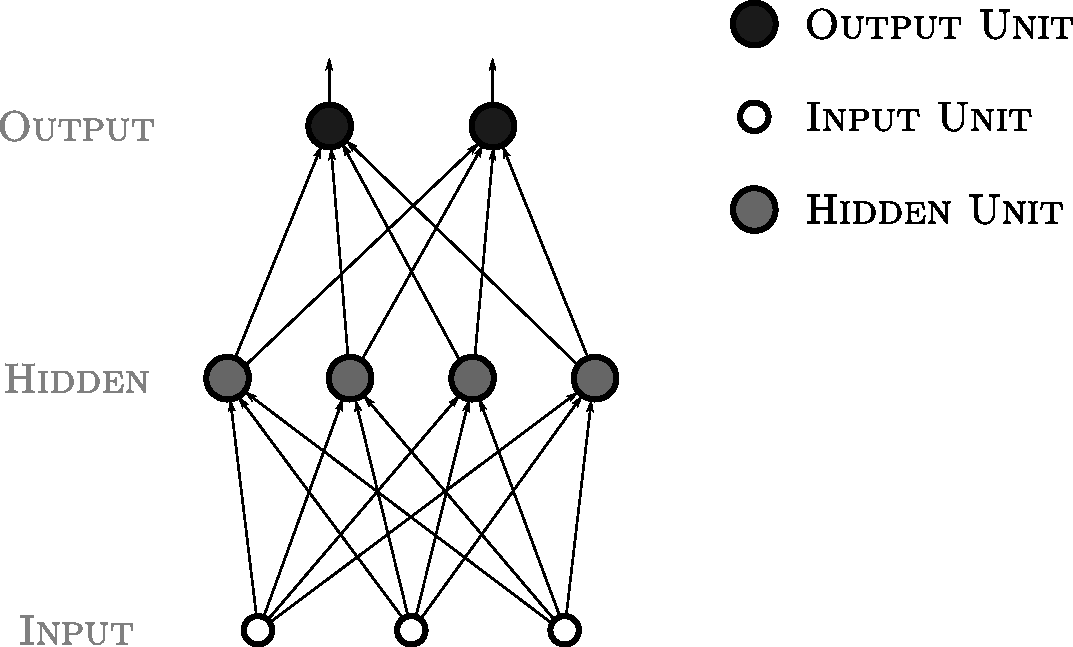
\includegraphics[width=0.7\columnwidth]{img/mlp}
\medskip
\caption[Multilayer Perceptron.]{Multilayer Perceptron. Architettura di una rete con 3 unità input, 2 unità di output e 4 unità nascoste, in un unico layer.}
\label{fig:intro:mlp}
\end{figure}

Come si vede dalle equazioni (\ref{eq:intro:neurone}) e (\ref{eq:intro:mlp}), i \emph{parametri liberi} di una Rete Neurale Artificiale sono rappresentati dai pesi, a valori reali, sulle connessioni: lo spazio delle ipotesi è dunque in questo caso continuo, il che permette di ascrivere il paradigma neurale alla classe degli approcci \emph{sub-simbolici} nel campo del Machine Learning. Sono invece detti \emph{iperparametri} di un modello i fattori che ne determinano lo spazio delle ipotesi (e.g.\ il numero di unità nascoste) o che influenzano l'apprendimento (e.g.\ i parametri dell'algoritmo di learning utilizzato).

Modelli di questo tipo si caratterizzano per la capacità di trattare efficacemente dati sia continui che discreti, realizzando task di classificazione o regressione, e mostrando tolleranza rispetto a dati di input rumorosi o incompleti.
La presenza di almeno un layer nascosto di unità con funzioni di attivazione non lineari (tipicamente sigmoidali, e.g.\ $\tanh$) ha inoltre l'effetto di rendere il Multilayer Perceptron un \emph{approssimatore universale} \cite{Cybenko:ApproximationBySuperpositions}, in grado cioè di approssimare con precisione arbitraria qualsiasi funzione continua definita su un sottoinsieme compatto di $\R^n$. 

L'apprendimento avviene generalmente, nelle Reti Neurali Feedforward, attraverso l'algoritmo di Backpropagation \cite{Haykin:NN}, che sfrutta una discesa del gradiente per modificare iterativamente i pesi di tutte le connessioni, minimizzando l'errore commesso sugli esempi etichettati di training. 


%%%%%%%%%%%%%%%%%%%%%%%%%%%%%%%%%%%%%%%%%%%
\subsection{Validazione}\label{intro:validazione}
Come detto in precedenza, lo scopo del processo di apprendimento in un modello di Machine Learning è quello di trovare una buona approssimazione, a partire da dati noti, all'interno di uno spazio di funzioni. Per definire cosa si intenda per \emph{buona} è necessario riferirsi alla capacità di \emph{generalizzazione}, ovvero all'accuratezza nel fare previsioni su dati sconosciuti.
La generalizzazione è dunque un punto determinante del Machine Learning e viene esplorata durante una fase di test in cui si esegue la valutazione dell'ipotesi in termini di capacità predittiva.

Per poter valutare la qualità dell'approssimazione di un modello si ricorre a delle funzioni di \emph{loss}
\begin{equation}
L(h(x), d) 
\end{equation}
che misurano la discrepanza tra l'output del modello ed il valore desiderato $d$ su un campione $x$ in ingresso (i.e.\ valori alti della loss indicano scarsa approssimazione).
Per i task di apprendimento supervisionato consideriamo le seguenti funzioni di loss:
\begin{itemize}
\item Classificazione: \emph{errore di classificazione}
\begin{equation}
L(h(x_i), d_i) =  
\begin{cases}
0 & \text{se } h(x_i) = d_i \\
1 & \text{altrimenti}
\end{cases}
\end{equation}
\item Regressione: \emph{errore quadratico}
\begin{equation}
L(h(x_i), d_i) =  (d_i - h(x_i))^2
\end{equation}
\end{itemize}

Il legame tra funzione di loss e generalizzazione è determinato dall'\emph{ipotesi dell'apprendimento induttivo}, secondo cui ogni ipotesi $h$ che approssima bene $f_t$ sugli esempi di training approssimerà bene $f_t$ anche su (nuove) istanze sconosciute di input.

Tale assunzione è fondante dell'approccio che si adotta nella realizzazione dell'apprendimento.
In accordo con tale ipotesi, per determinare l'approssimazione migliore di $f_t$, si ricerca quindi un'ipotesi $h$ che minimizzi l'\emph{errore reale} $R$
\begin{equation}
R = \int L(d, h(x))\, dP(x,d)  
\end{equation}
dove $d$ è un valore dato dal teacher, $P(x,d)$ è la distribuzione dei dati --- che generalmente non è nota a priori --- e $L(d, h(x))$ è una funzione di loss.\\
Disponendo solo di un insieme finito di dati di training
\begin{equation} 
D = \lbrace (x_i, d_i) \rbrace_{i=1}^{l}  
\end{equation}
per cercare $h$ si ricorre alla minimizzazione del \emph{rischio empirico} (errore di training), alla ricerca dei migliori valori per i parametri liberi del modello
\begin{equation}
R_{emp} = \frac{1}{l} \sum_{i} L(d_i, h(x_i))
\end{equation}
seguendo il principio induttivo della \emph{Minimizzazione del Rischio Empirico}.

Esiste tuttavia la possibilità che l'ipotesi dell'apprendimento induttivo non sia fondata, in particolare nel caso di \emph{overfitting}.
Considerando un'ipotesi generica $h_i \in H$ e chiamando $\epsilon_i$ il suo errore reale e $E_i$ il suo errore empirico, diciamo che un learner fa \emph{overfitting} se l'ipotesi in output $h_{out}$ è tale che esiste una ipotesi diversa $h_j \in H$ per cui: $E_{out} < E_j$ e $\epsilon_{out} > \epsilon_j $.
Intuitivamente, quindi, l'overfitting corrisponde alla situazione in cui un modello sia stato allenato fino a raggiungere un livello di approssimazione dei dati di training eccessivamente alto, perdendo di conseguenza la capacità di generalizzare.

In modo particolare nell'uso di Reti Neurali, caratterizzate da un'estrema flessibilità nell'approssimare la funzione obiettivo, si rende dunque necessario un procedimento che permetta di valutare con accuratezza la performance di un modello. Nel seguito vengono brevemente descritte alcune delle tecniche comunemente usate a questo scopo (si veda anche \cite{Hastie:EOSL}).

\subsubsection*{Hold-out}
Questa tecnica può essere utilizzata qualora si disponga di dataset di grosse dimensioni, e rappresenta il caso più semplice di validazione di un modello.

Il dataset $D$ viene partizionato in due insiemi \emph{disgiunti}: un \emph{training-set} $D_\textup{tr}$ ed un \emph{test-set} $D_\textup{ts} = D \setminus D_\textup{tr}$. Si ha dunque
\[
D = D_\textup{tr} \cup D_\textup{ts} 
% \quad \text{e} \quad D_\textup{tr} \cap D_\textup{ts} = \emptyset
\]
Il modello viene allenato sul training-set e, successivamente, il test-set viene utilizzato per valutarne la capacità di generalizzazione. 

Per garantire che i risultati possano essere rappresentativi della capacità predittiva del modello, il test-set non viene usato per l'adattamento dei parametri liberi né per la selezione del modello (i.e.\ scelta degli iperparametri). A questo scopo, se si hanno maggiori dati a disposizione, è possibile partizionare ulteriormente il training-set, ottenendo un \emph{validation-set} $D_\textup{val}$ che può essere usato per scegliere l'ipotesi migliore. In questo caso, quindi si ha
\[
D = D_\textup{tr} \cup D_\textup{val} \cup D_\textup{ts} 
%\quad \text{e} \quad 
%D_\textup{tr} \cap D_\textup{val} \cap D_\textup{ts} = \emptyset
\]
con i dati in $D_\textup{tr}$ usati per allenare più modelli, $D_\textup{val}$ impiegato per scegliere, fra i vari modelli allenati, quello considerato più adatto al problema affrontato ed, infine, $D_\textup{ts}$ usato per determinare la performance del modello scelto. Il processo di scelta dell'ipotesi migliore attraverso un validation-set è chiamato \emph{model selection} ed avviene dunque secondo un procedimento di \emph{trial and error}.

\subsubsection*{K-fold cross-validation}
Nel caso in cui si abbiano pochi dati a disposizione, l'hold-out può comportare una riduzione eccessiva di dati utili per il training. In questo caso si procede con la variante della \emph{k-fold cross-validation}, che prevede il partizionamento del dataset $D$ in $k$ sottoinsiemi, o \emph{fold}, mutuamente esclusivi
\[
D = D_1 \cup D_2 \cup \dots \cup D_k
%\quad \text{e} \quad 
%D_1 \cap D_2 \cap \dots \cap D_k = \emptyset
\]
Il modello viene dunque allenato e testato per $k$ volte, facendo in modo che la porzione di dati usati per il test non sia usata nel training del modello
\[
D_\textup{tr} = D \setminus D_i
\quad \text{e} \quad 
D_\textup{ts} = D_i
\qquad \text{per} \quad i=1,\dots,k
\]
La performance è infine ottenuta come media delle performance ottenute sul test-set delle varie fold.

L'impiego di k-fold cross-validation consente dunque di usare tutti i dati a disposizione sia per il training che per il test e può essere combinato, come nel caso dell'hold-out, con l'uso di un validation-set per la selezione del modello.

\subsubsection*{Double k-fold cross-validation}
In questo caso vengono realizzati due cicli di cross-validation, di cui quello ``interno'' viene utilizzato per la selezione del modello.

Come per la k-fold cross-validation, il dataset viene inizialmente partizionato in fold
\[
D = D_1 \cup D_2 \cup \dots \cup D_k
%\quad \text{e} \quad 
%D_1 \cap D_2 \cap \dots \cap D_k = \emptyset
\]
e successivamente, ogni fold viene a sua volta suddivisa in $t$ sotto-fold
\[
D_i = D_{i1} \cup D_{i2} \cup \dots \cup D_{it}
%\quad \text{e} \quad 
%D_{i1} \cap D_{i2} \cap \dots \cap D_{it} = \emptyset
\qquad \text{per} \quad i=1,\dots,k
\]
Ogni sotto-fold viene dunque utilizzata per allenare e valutare più iperparametrizzazioni
\[
D_\textup{tr} = D_i \setminus D_{ij}
\quad \text{e} \quad 
D_\textup{val} = D_{ij}
\qquad \text{per} \quad j=1,\dots,t
\]
Tale processo permette di ottenere $k$ modelli ``vincenti'', uno per ogni fold, selezionati in base alla performance media sui validation-set. Il test viene dunque eseguito, su ogni fold, valutando il modello vincente attraverso una k-fold cross-validation
\[
D_\textup{tr} = D \setminus D_i
\quad \text{e} \quad 
D_\textup{ts} = D_i
\qquad \text{per} \quad i=1,\dots,k
\]
La performance del modello è quindi calcolata come la media delle performance raggiunte dalle iperparametrizzazioni vincenti su ogni fold.

La double k-fold cross-validation è un processo accurato, ma computazionalmente dispendioso, che consente di ottenere una stima dell'accuratezza di un modello anche su dataset di dimensioni ridotte. Si distingue tuttavia dalle tecniche precedenti per il fatto di restituire non una, ma $k$, iperparametrizzazioni vincenti.

\subsubsection*{Stratificazione}
Nel partizionare un dataset secondo le tecniche descritte è ovviamente necessario che tutti i sottoinsiemi siano sufficientemente rappresentativi per il problema trattato e che riescano dunque a descrivere le relazioni fra i dati. Eventuali sbilanciamenti nella natura dei dati in uno dei sottoinsiemi possono infatti comportare un \emph{bias} che può avere impatto negativo sulla capacità di generalizzazione dei modelli.

La \emph{stratificazione} è una tecnica mirata ad evitare questo scenario e prevede che i dati vengano partizionati, prima del sampling, in gruppi omogenei, in modo che i sottoinsiemi possano essere formati mantenendo lo stesso rapporto fra i gruppi presente nell'intero dataset. 


%%%%%%%%%%%%%%%%%%%%%%%%%%%%%%%%%%%%%%%%%%%
\subsection{Algoritmi di apprendimento}\label{intro:alg}
In questo paragrafo sono riportati alcuni degli algoritmi di apprendimento che verranno riferiti nel seguito e che sono stati utilizzati nel corso del lavoro svolto. Gli algoritmi coprono un caso specifico dell'apprendimento nell'ambito neurale: l'allenamento di singole unità che operano come il neurone artificiale descritto nell'equazione (\ref{eq:intro:neurone}).

Quanto verrà descritto non si rivolge dunque all'adattamento dei pesi di una rete multistrato (si veda il paragrafo~\ref{intro:ann}), che richiede tecniche specifiche, quanto l'allenamento di un singolo livello di output. Per questo motivo, gli algoritmi riportati si caratterizzano per la loro semplicità ed efficienza computazionale.

\subsubsection*{Least Mean Squares}
Consideriamo un'unità con una funzione di attivazione non lineare e differenziabile (e.g.\ $\tanh$) che abbia $\N_U$ ingressi. Possiamo scrivere l'uscita per l'input $\vect{x} \in \R^{N_U}$ come
\begin{equation}
o(\vect{x}) = f(\transpose{\vect{x}}\vect{w})
\end{equation}
dove $\vect{w} \in \R^{N_U}$ rappresenta il vettore dei pesi associati ai singoli input.\\
Siamo interessati a determinare un valore appropriato per $\vect{w}$, che minimizzi la somma degli errori al quadrato
\begin{equation}\label{eq:lms:error}
E(\vect{w}) = \sum_p (d_p - o(\vect{x}_p))^2 = \sum_p (d_p - f(\transpose{\vect{x}_p} \vect{w}) )^2 
\end{equation}
Utilizzando l'algoritmo Least Mean Squares (LMS) \cite{Haykin:NN} la minimizzazione procede attraverso un \emph{discesa del gradiente}
\begin{equation}
-\Delta\vect{w} = 
\frac{\partial{E(\vect{w})}}{\partial{w_j}} = 
-2 \sum_{p \rightarrow l } (\vect{x}_p)_j 
(d_p - f(\transpose{\vect{x}_p} \vect{w})) f'(\transpose{\vect{x}_p} \vect{w})
\end{equation}
Iterativamente, i pesi $\vect{w}$ vengono dunque modificati come
\begin{equation} 
\vect{w}_{new} = \vect{w}_{old} + \eta\, \Delta\vect{w}_{old}
\end{equation}
dove $\eta$ è il \emph{learning-rate}, iperparametro dell'algoritmo. Ad ogni iterazione, il costo dell'algoritmo è lineare rispetto alla dimensione dell'input $N_U$.

Il procedimento si può inoltre estendere, aggiungendo alla funzione di errore un fattore di penalizzazione che impedisca ai
pesi di assumere valori troppo alti, in accordo con il principio della \emph{minimizzazione del rischio strutturale} \cite{Vapnik:RiskMinimization}. L'aumento del valore dei pesi corrisponde infatti ad un aumento della complessità del modello, che favorisce il verificarsi di situazioni di overfitting.\\
In questo caso l'aggiornamento dei pesi viene modificato in
\begin{equation} 
\vect{w}_{new} = \vect{w}_{old} + \eta\, \Delta\vect{w}_{old} - \lambda_\textup{wd}\, \vect{w}_{old}
\end{equation}
dove $\lambda_\textup{wd}$ è un parametro corrispondente al cosiddetto \emph{weight decay}.\\
La riduzione della complessità del modello viene chiamata \emph{regolarizzazione}.



%%%%%%%%%%%%%%%%%%%%%%%%%%%%%%%%%%%%%%%%%%%
\subsubsection*{Ridge Regression}
Consideriamo un insieme di $\abs{D}$ vettori di input rappresentati in forma matriciale, $\matr{X} \in \R^{\abs{D} \times N_U}$, ed un insieme di output desiderati, o valori target, $\matr{Y}_\textup{target} \in \R^{\abs{D} \times N_Y}$.
L'algoritmo di Ridge Regression \cite{Hastie:EOSL} permette di calcolare i pesi di $N_Y$ unità con funzione di attivazione lineare, in modo da minimizzare l'errore (\ref{eq:lms:error}) e tenendo conto di un fattore di penalizzazione, come nel caso di LMS con weight decay.\\
La matrice dei pesi, $\matr{W} \in \R^{N_U \times N_Y}$, è in questo caso calcolata come
\begin{equation}
\matr{W} = (\matr{X}^T \matr{X} + \lambda_\textup{r} \matr{I})^{-1} \matr{X}^T \matr{Y}_\textup{target}
\end{equation}
dove $\matr{I} \in \R^{N_U \times N_U}$ è la matrice identità e $\lambda_\textup{r}$ è un parametro di regolarizzazione.

A differenza di LMS, l'algoritmo di Ridge Regression permette di ottenere la soluzione in maniera diretta, senza ricorrere ad un procedimento iterativo. Il costo computazionale dell'algoritmo è cubico rispetto alla dimensione dell'input $N_U$.

Benché sia definito su unità lineari, è possibile applicare l'algoritmo al caso di unità con funzioni di attivazioni non lineari semplicemente modificando i valori target, applicando $f^{-1}$ elemento per elemento: $\matr{Y}_\textup{target}' = f^{-1}(\matr{Y}_\textup{target})$. In questo caso è ovviamente necessario che la funzione di attivazione sia invertibile e che i valori target rientrino nel suo codominio.


%%%%%%%%%%%%%%%%%%%%%%%%%%%%%%%%%%%%%%%%%%%%%%%%%%%%%%%%%%%%%%%
%%%%%%%%%%%%%%%%%%%%%%%%%%%%%%%%%%%%%%%%%%%%%%%%%%%%%%%%%%%%%%%

\section{Reti Neurali Costruttive}\label{sec:intro:cnn}
La maggior parte degli algoritmi per Reti Neurali Artificiali prevede l'uso di modelli con architetture statiche. Più esattamente, reti con una topologia prefissata vengono create e successivamente allenate: i pesi sulle connessioni vengono fatti variare, ma non l'architettura in sé.\\
Uno degli evidenti svantaggi di un simile approccio sta nella necessità di dover evitare i casi in cui la rete risulti essere, per la propria struttura e quindi al netto delle modifiche ai pesi, troppo o troppo poco complessa per il task che si vuole affrontare.

Le \emph{Reti Neurali Costruttive} \cite{Smieja:NeuralNetworkConstructive,Prechelt:InvestigationOfTheCasCor} offrono una valida soluzione al problema di dover stabilire a priori la topologia della rete affinché possa ben adattarsi al task che si vuole risolvere. L'allenamento di una rete neurale costruttiva inizia tipicamente con una rete di piccole dimensioni --- anche senza alcuna unità nascosta, nel caso delle reti feedforward --- e procede aggiungendo nuove unità alla rete finché questa non abbia raggiunto una complessità compatibile con il problema in questione.

Al di là dei dettagli implementativi possiamo dunque individuare le due caratteristiche alla base dell'approccio costruttivo.
\begin{itemize}
\item Una rete viene vista come formata da più \emph{unità computazionali} con una capacità limitata, che vengono allenate per risolvere un sotto-problema rispetto al task affrontato.
\item La rete \emph{aumenta la propria complessità} nel corso del training, adattandosi al task che le viene sottoposto.
\end{itemize}
\`E importante sottolineare come questi due principi, benché sviluppati nell'ambito delle Reti Feedforward, possano essere applicabili ad un'ampia classe di problemi o modelli.

I principali vantaggi offerti dall'adozione di un approccio costruttivo sono:
\begin{itemize}
\item Il superamento della necessità di dover fissare a priori la topologia della rete, che diventa dunque adattiva e viene dinamicamente ``appresa'' dalla rete stessa.
\item La possibilità di definire per le sotto-reti dei task specifici, che possano essere trattati in maniera più efficace o più efficiente rispetto al problema affrontato.
\item L'adozione di una politica locale nell'aggiornamento dei pesi, con il duplice vantaggio di evitare i problemi legati all'adattamento dei pesi dell'intera rete (e.g.\ \emph{vanish del gradiente}) e di consentire l'implementazione di meccanismi di caching/memoization per le porzioni di rete non direttamente interessate dal learning locale.
\item La possibilità di circoscrivere il learning ad unità computazionali, o sotto-reti, più semplici della rete nel suo complesso. Questo consente in particolare l'impiego di algoritmi di apprendimento specifici e meno onerosi dal punto di vista computazionale rispetto a quelli necessari ad allenare l'intera rete.
\end{itemize}

A fronte dei vantaggi offerti, le Reti Neurali Costruttive presentano tuttavia alcune criticità legate alla capacità della rete di crescere. Poiché generalmente ogni nuova unità è connessa alle precedenti, infatti, le reti di grandi dimensioni tendono ad avere molti layer ed unità con un un numero di connessioni in input molto elevato: questo può avere un grosso impatto sul processo di learning e compromettere la scalabilità del modello. Il fatto che la rete possa aumentare il proprio numero di unità indefinitamente, guidata unicamente dall'input, espone inoltre i modelli costruttivi al verificarsi di situazioni di overfitting (si veda il paragrafo~\ref{intro:validazione}).




%%%%%%%%%%%%%%%%%%%%%%%%%%%%%%%%%%%%%%%%%%%%%%%%%%%%%%%%%%%%%%%
\subsection{Cascade Correlation}\label{sec:intro:cnn:ccorr}

L'algoritmo \emph{Cascade Correlation} \cite{Fahlman:CC, Littmann:learningAndGeneralization, Prechelt:InvestigationOfTheCasCor} rappresenta probabilmente uno dei più diffusi casi di applicazione dell'approccio costruttivo nell'allenamento di Reti Neurali Feedforward. L'intuizione alla base dell'algoritmo sta nell'idea di allenare nuove unità computazionali perché possano (i) contribuire alla risoluzione del task affrontato risolvendo dei sotto-problemi di natura diversa e semplificata e (ii) avvalersi delle informazioni precedentemente apprese dalla rete nel corso del processo costruttivo. In particolare ad ogni nuova unità viene affidato il compito di \emph{massimizzare la correlazione} fra il proprio output e l'errore commesso dalla rete, con lo scopo di correggerlo.

L'evoluzione dell'algoritmo è la seguente. Inizialmente la rete non ha unità nascoste; le connessioni input--output vengono dunque allenate sul training-set attraverso un algoritmo di apprendimento adatto a reti con un singolo strato (e.g.\ \textit{delta-rule} o algoritmo di apprendimento del Perceptron) e senza necessità di utilizzare Backpropagation.

Dopo aver effettuato l'allenamento viene calcolato l'errore commesso dalla rete: se si è soddisfatti della performance raggiunta, in termini di fitting, allora l'algoritmo termina, altrimenti si procede nel tentativo di ridurre l'errore.

Per ridurre l'errore, una nuova unità nascosta, chiamata \emph{candidata}, viene aggiunta alla rete: collegata sia all'input che ad ogni altra unità nascosta esistente, viene allenata perché il suo output abbia correlazione massima con l'errore residuo commesso dalla rete. La correlazione (non normalizzata) $S$ fra l'uscita della rete $V$ e l'errore residuo $E_o$ osservato all'unità di output $o$-esima è definita come
\begin{equation}\label{eq:S}
S = \sum_o \left\lvert \sum_p (V_p - \bar{V}) (E_{p,o} - \bar{E}_o) \right\rvert
\end{equation}
dove $p$ indica i pattern in input e $\bar{V}$ ed $\bar{E}_o$ sono i valori medi, dell'uscita e dell'errore rispettivamente, calcolati su tutti i pattern del training-set.\\
L'allenamento della candidata avviene attraverso una \emph{ascesa del gradiente} che sfrutta la derivata parziale di $S$ rispetto al generico peso $w_i$
\begin{equation}
\dfrac{\partial S}{\partial w_i} = \sum_{p,o} \sigma_o \, (E_{p,o} - \bar{E}_o)\, f'_p \, I_{i,p}
\end{equation}
dove $\sigma_o$ è il segno della correlazione fra l'output della candidata e l'output $o$, $f'_p$ è la derivata della funzione di attivazione della candidata (e.g.\ tangente iperbolica) applicata ai suoi input per il pattern $p$-esimo ed $I_{i,p}$ è l'$i$-esimo input che la candidata riceve per il pattern $p$.\\
In questa fase è inoltre possibile ricorrere all'uso di un \emph{pool} di unità candidate, ognuna con pesi iniziali random, in modo da variare le condizioni iniziali dell'algoritmo di apprendimento e scegliere poi l'unità che abbia raggiunto il massimo valore di $S$.

\begin{figure}[tbp]
\centering
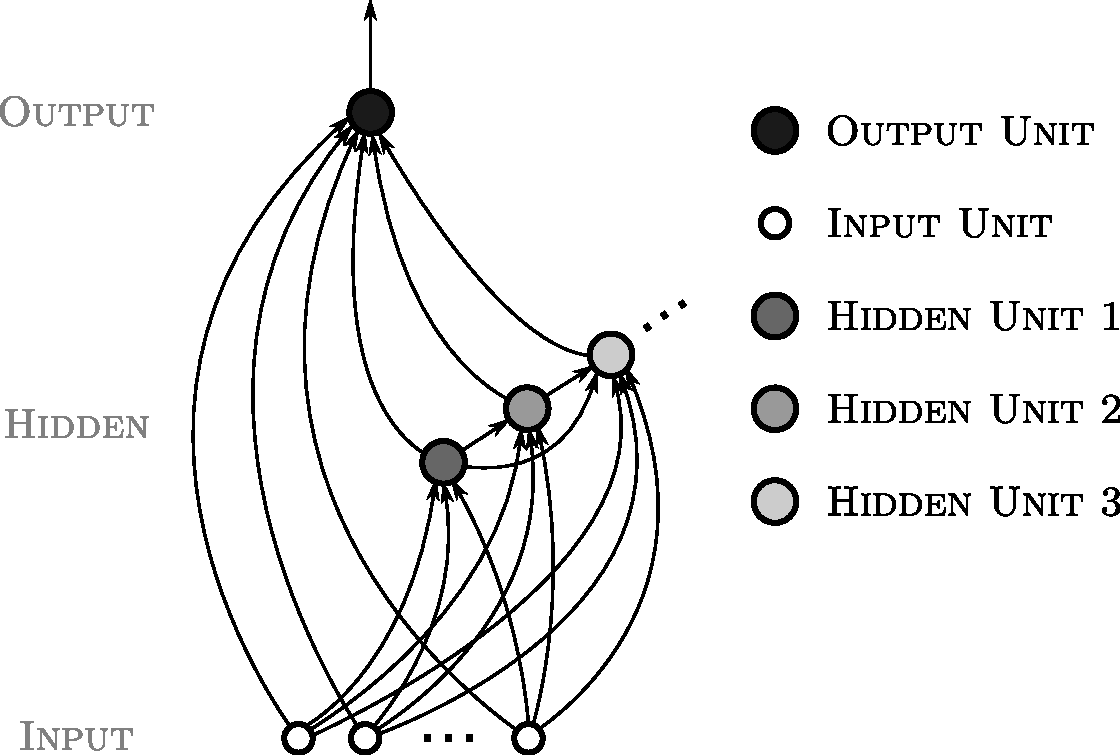
\includegraphics[width=0.6\columnwidth]{img/cascorr}
\medskip
\caption[Cascade Correlation.]{Cascade Correlation. Architettura di una rete con 1 unità di output e 3 unità nascoste.}
\label{fig:intro:cascorr}
\end{figure}

Ad apprendimento ultimato la nuova unità viene stabilmente aggiunta alla rete: i pesi sulle sue connessioni in ingresso vengono ``congelati'', di modo che rimarranno inalterati per il resto del processo di costruzione della rete, ed il suo output viene collegato allo strato di output della rete. Il ``congelamento'' dei pesi sulle connessioni in input alla nuova unità ha risvolti importanti sulle caratteristiche dell'algoritmo. Una volta allenata, infatti, l'unità candidata agirà permanentemente come un \emph{feature detector} e la sua uscita potrà essere presentata allo strato di output o ad altre unità nascoste esattamente come un input aggiuntivo. Benché la rete evolva secondo una architettura a più layer (i.e.\ ogni unità rappresenta un layer a sé stante, figura~\ref{fig:intro:cascorr}), dunque, gli input e le uscite delle unità nascoste possono essere considerati come appartenenti ad un unico strato ai fini dell'allenamento, il che permette l'uso di algoritmi di apprendimento semplici e poco onerosi dal punto di vista computazionale.

Aggiunta una nuova unità nascosta si procede nuovamente con l'allenamento delle connessioni verso l'output della rete, con la valutazione dell'errore commesso ed eventualmente con l'aggiunta di nuove unità, finché il fitting non sia ritenuto soddisfacente. L'algoritmo evolve dunque in maniera \emph{greedy}, aggiungendo unità nascoste finché non siano rispettati determinati criteri di stop.

Per chiarire meglio in che modo evolve la topologia di una rete allenata con Cascade Correlation, la figura~\vref{fig:intro:cascorr} mostra l'architettura di una rete con 3 unità nascoste ed un'unica unità di output.


%%%%%%%%%%%%%%%%%%%%%%%%%%%%%%%%%%%%%%%%%%%%%%%%%%%%%%%%%%%%%%%
%%%%%%%%%%%%%%%%%%%%%%%%%%%%%%%%%%%%%%%%%%%%%%%%%%%%%%%%%%%%%%%
\section{Reti Neurali Ricorrenti}\label{sec:intro:rnn}
Le Reti Neurali Ricorrenti \cite{Tsoi:DiscreteTimeRNN, Haykin:NN} generalizzano le Reti Neurali Feedforward (si veda il paragrafo~\ref{sec:intro:MLeNN}) al trattamento di sequenze. Ciò che distingue le due classi di modelli risiede nel fatto che le Reti Neurali Ricorrenti presentano cicli nella topologia delle connessioni. Questa semplice caratteristica ha un profondo impatto sulle proprietà della rete, in particolare:
\begin{itemize}
\item Per effetto dei cicli nella struttura  delle connessioni, una Rete Neurale Ricorrente può sviluppare e mantenere delle dinamiche interne anche in assenza di input. Reti di questo tipo realizzano infatti un \emph{sistema dinamico}, mentre le Reti Neurali Feedforward realizzano \emph{funzioni}.
\item Se guidate da un segnale di ingresso, le Reti Neurali Ricorrenti mantengono nel proprio stato interno (i.e.\ nelle attivazioni delle proprie unità) una trasformazione non lineare del passato dell'input. La rete possiede dunque una \emph{memoria dinamica} che le permette di elaborare informazioni in un contesto temporale.
\end{itemize}
Grazie all'introduzione di cicli nella topologia, dunque, la rete può essere usata per elaborare dati sequenziali realizzando una \emph{trasduzione di sequenza}, ovvero una funzione da un dominio di sequenze di input ad un dominio di sequenze di output. 

Nella sua forma più semplice una Rete Neurale Ricorrente è composta da un layer di ingresso, un successivo layer nascosto ricorrente (i.e.\ con connessioni cicliche fra le unità) ed un ultimo layer feedforward (i.e.\ con connessioni acicliche) di uscita: il layer nascosto calcola una \emph{funzione locale di encoding} dell'input, mentre il layer di output calcola una \emph{funzione di output}.
Per realizzare l'encoding, in una rete che abbia $N_U$ unità di input ed $N_R$ unità nascoste, il layer nascosto calcola la \emph{funzione di transizione di stato} ricorrente $\tau : \R^{N_U} \times \R^{N_R} \rightarrow \R^{N_R}$ come
\begin{equation}\label{intro:rnn:encoding}
\vect{x}(n) = \tau(\vect{u}(n), \vect{x}(n-1) ) = f( \matr{W}_\textup{in} \vect{u}(n) + \hat{\matr{W}} \vect{x}(n-1) )
\end{equation}
dove $f$ è la funzione di attivazione tipicamente sigmoidale delle unità nascoste, $\vect{u}(n)$ rappresenta l'input $n$-esimo della sequenza, $\vect{x}(t)$ è lo stato interno della rete (i.e.\ le attivazioni delle unità nascoste), la matrice $\matr{W}_\textup{in} \in \R^{N_R \times (N_U + 1)}$ contiene i pesi sulle connessioni dal livello di input al livello nascosto (compreso un \emph{bias}) e la matrice $\hat{\matr{W}} \in \R^{N_R \times N_R}$ contiene i pesi sulle connessioni ricorrenti fra le unità nascoste.\\
Per una rete che abbia $N_Y$ unità di uscita, il layer di output calcola invece la funzione di output $g_\textup{out} : \R^{N_R} \rightarrow \R^{N_Y}$ come
\begin{equation}\label{intro:rnn:output}
\vect{y}(n) = g_\textup{out}(\vect{x}(n)) = f_\textup{out}(\matr{W}_\textup{out} \vect{x}(n))
\end{equation}
dove $\vect{y}(n)$ è l'uscita della rete al passo $n$-esimo, $f_\textup{out}$ è la funzione di attivazione delle unità di output e $\matr{W}_\textup{out} \in \R^{N_Y \times (N_R + 1)}$ contiene i pesi delle connessioni fra il layer nascosto ed il layer di output (più il \emph{bias}).

L'allenamento delle Reti Neurali Ricorrenti usa generalmente tecniche di discesa del gradiente in cui tutte le connessioni della rete vengono modificate per minimizzare l'errore. Gli algoritmi di apprendimento più comuni sono \emph{Back Propagation Through Time} (BPTT) \cite{Werbos:BPTT} e \emph{Real-Time Recurrent Learning} (RTRL) \cite{Williams:RTRL}, che estendono al caso ricorrente le tecniche applicate per l'allenamento di Reti Neurali Feedforward, sfruttando la costruzione di una rete multistrato con topologia aciclica, ottenuta ``copiando'' il layer nascosto, ricorrente, della rete lungo ogni passo della sequenza temporale di input (\emph{unfolding}) \cite{Rumelhart:LearningInternal}.



%%%%%%%%%%%%%%%%%%%%%%%%%%%%%%%%%%%%%%%%%%%%%%%%%%%%%%%%%%%%%%%
%%%%%%%%%%%%%%%%%%%%%%%%%%%%%%%%%%%%%%%%%%%%%%%%%%%%%%%%%%%%%%%

\section{Reservoir Computing}\label{sec:intro:rc}
Il \emph{Reservoir Computing} \cite{Lukosevicius:ESN-Survey,Verstraeten:AnExperimentalUnification,Jaeger:HarnessingNonlinearity} è un paradigma emergente, nell'ambito delle \emph{Reti Neurali Ricorrenti}, che ha origine da due classi di modelli: \emph{Echo State Networks} (ESN) \cite{Jaeger:EchoStateApproach} e \emph{Liquid State Machines} (LSM) \cite{Maas:LSM}.
Benché entrambi i modelli condividano --- e contribuiscano a definire --- i tratti distintivi del Resevoir Computing, nel seguito si farà riferimento in maniera specifica alle ESN, maggiormente legate ad un approccio computazionale\footnote{Le LSM nascono infatti nell'ambito delle neuroscienze e mantengono caratteristiche di forte ispirazione biologica.} e vere progenitrici dei modelli oggetto del lavoro svolto.\\
Prima di descrivere il funzionamento di una ESN, è utile delineare motivazioni, intuizioni e metodi che caratterizzano il Reservoir Computing come paradigma a sé stante per il trattamento di dati strutturati\footnote{Il termine \emph{dati strutturati} è in questo contesto volutamente generico. Benché in questo paragrafo ci si riferisca a dati in forma di sequenze, dominio proprio delle Reti Neurali Ricorrenti e quindi delle ESN, è vero infatti che le caratteristiche del paradigma possono essere riportate a domini strutturati anche più complessi, come i grafi (si veda il paragrafo~\vref{sec:intro:struct:gesn}).}.

Riprendendo quanto descritto nel paragrafo~\ref{sec:intro:rnn}, una generica Rete Neurale Ricorrente viene usata per elaborare dati sequenziali apprendendo una \emph{trasduzione di sequenza}. Tale compito è realizzato modellando un sistema dinamico in cui lo stato interno e l'uscita sono determinati come definito nelle equazioni (\ref{intro:rnn:encoding}) e (\ref{intro:rnn:output}) rispettivamente.
Osservando le formule risulta evidente come l'encoding e l'output giochino un ruolo differente: la \emph{funzione di transizione di stato} $\tau$ implementa infatti un processo di codifica ricorsivo della sequenza in input, che sfrutta informazioni sul contesto ed ha quindi una propria memoria, mentre $\vect{y}(n)$ è il risultato di una funzione pura, senza memoria, della codifica in $\vect{x}(n)$. 

Secondo l'approccio classico, l'allenamento delle Reti Neurali Ricorrenti usa tecniche di discesa del gradiente che prevedono l'adattamento di tutti i pesi della rete: nessuna suddivisione concettuale fra stato interno ed output viene realizzata benché le differenze emergano dal punto di vista algoritmico (l'output, a differenza dello stato interno, è infatti direttamente confrontabile con il target). Gli algoritmi di apprendimento più comuni, \emph{Back Propagation Through Time} (BPTT) \cite{Werbos:BPTT} e \emph{Real-Time Recurrent Learning} (RTRL) \cite{Williams:RTRL}, soffrono tuttavia di alcuni svantaggi. In particolare:
\begin{itemize}
\item L'aggiornamento graduale dei parametri può modificare le dinamiche della rete fino a far degenerare le informazioni del gradiente, di modo che la convergenza possa non essere garantita \cite{Doya:Bifurcations}.
\item Il costo computazionale per l'aggiornamento è molto alto ---  $O(N^2)$ per BPTT e $O(N^4)$ per RTRL, in una rete con $N$ unità --- e riduce la possibilità di utilizzare reti di grandi dimensioni.
\item Il gradiente decresce esponenzialmente nel tempo, per cui risulta difficile apprendere dipendenze a lungo termine \cite{Bengio:TheProblemOfLearning}.
\end{itemize}

Il paradigma del Reservoir Computing nasce dunque con l'idea di evitare almeno parzialmente questi problemi adottando un approccio radicalmente differente:
\begin{itemize}
\item Una rete neurale ricorrente, chiamata \emph{reservoir}, viene generata \emph{in maniera casuale} ed ha lo scopo di espandere il segnale in input, mantenendo nel proprio stato interno una trasformazione non lineare del passato. I pesi del reservoir rimangono \emph{inalterati} durante il training. 
\item L'output viene generato come una \emph{combinazione lineare} dei segnali provenienti dalle unità del reservoir, passivamente eccitate dall'input. Il \emph{readout} lineare viene adattato, in fase di learning, utilizzando il segnale del teacher come target.
\end{itemize}
La suddivisione fra stato interno della rete ed output è quindi in questo caso resa esplicita e si sfrutta la capacità del reservoir di mantenere una trasformazione non lineare del passato, anche senza dover effettuare l'apprendimento \cite{Tino:MarkovianArchitecturalBias}, per limitare l'azione del learning al solo readout.

Benché il Reservoir Computing si caratterizzi come un paradigma a sé, è giusto osservare che l'idea di gestire in maniera specifica e separata readout e stato interno trova altri esempi nell'ambito del Machine Learning: è il caso, ad esempio, dell'algoritmo di apprendimento \emph{Backpropagation-Decorrelation}\footnote{Per le sue caratteristiche, l'algoritmo BPDC viene talvolta indicato a tutti gli effetti come appartenente all'ambito del Reservoir Computing. Si veda, ad esempio, \cite{Song:Effects}.} (BPDC) \cite{Steil:BPDC} o delle \emph{Extreme Learning Machines} (ELM) \cite{Huang:ELM}. In termini ancor più generali, l'approccio del Reservoir Computing è inoltre riconducibile all'utilizzo di un kernel, come sottolineato anche in \cite{Jaeger:SpecialIssue}. 


%%%%%%%%%%%%%%%%%%%%%%%%%%%%%%%%%%%%%%%%%%%%%%%%%%%%%%%%%%%%%%%
\subsection{Echo State Networks}\label{sec:intro:rc:esn}
Definiamo formalmente le ESN \cite{Jaeger:EchoStateApproach, Jaeger:ShortTermMemory, Jaeger:HarnessingNonlinearity}, fissando anche parte della terminologia che verrà adottata nel seguito.

Consideriamo una rete con $N_U$ unità di input, $N_R$ unità ricorrenti interne (reservoir), ed $N_Y$ unità di output. 
Indichiamo con $\vect{u}(n) \in \R^{N_U}$ l'input all'istante $n$, appartenente alla sequenza $s(\vect{u}) = [\vect{u}(1), \vect{u}(2), \dots, \vect{u}(k)]$, con $\vect{x}(n) \in \R^{N_R}$ le attivazioni delle unità del reservoir e con $\vect{y}(n) \in \R^{N_Y}$ l'output.\\
Usiamo le seguenti matrici per i pesi delle connessioni: $\matr{W}_\textup{in} \in \R^{N_R \times (N_U+1)}$ per l'input, $\matr{W} \in \R^{N_R \times N_R}$ per le connessioni interne e $\matr{W}_\textup{out} \in \R^{N_Y \times (N_R+1)}$ per le connessioni verso le unità di output, ovvero verso il readout.\\
Le equazioni di base che determinano l'evoluzione del sistema sono le seguenti:
\begin{equation}\label{eq:intro:esn}
\begin{array}{l}
\vect{x}(n) = \tau( \vect{u}(n), \vect{x}(n-1) ) = f( \matr{W}_{\textup{in}} \vect{u}(n) + \hat{\matr{W}} \vect{x}(n-1) ) \\
\vect{y}(n) = g_\textup{out}( \vect{x}(n) ) = f_{\textup{out}}( \matr{W}_{\textup{out}} \vect{x}(n) )
\end{array}
\end{equation}
dove $f$ ed $f_{\textup{out}}$ sono funzioni applicate elemento per elemento e corrispondono rispettivamente alle funzioni di attivazione delle unità del reservoir, tipicamente sigmoidali (e.g.\ $\tanh$), e delle unità di output, tipicamente lineari.
La figura~\ref{fig:intro:esn} mostra in maniera schematica la struttura di una ESN come quella descritta dall'equazione (\ref{eq:intro:esn}).

\begin{figure}[tbp]
\centering
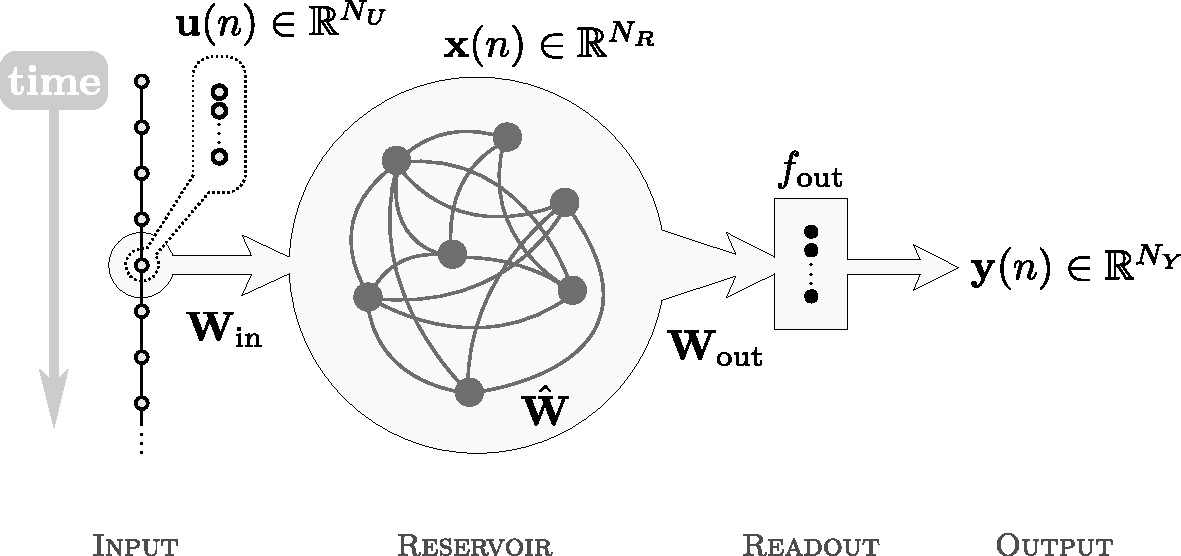
\includegraphics[width=0.8\columnwidth]{img/ESN}
\medskip
\caption[Echo State Network.]{Schematizzazione grafica di una Echo State Network (ESN).}
\label{fig:intro:esn}
\end{figure}

Varianti comuni all'equazione (\ref{eq:intro:esn}) prevedono inoltre l'esistenza di connessioni dirette dall'input al readout o all'indietro, dal readout al reservoir (si veda ad esempio \cite{Jaeger:EchoStateApproach, Jaeger:ShortTermMemory}). La presenza di queste ultime in particolare implica considerazioni specifiche e risulta interessante ai fini del lavoro svolto. L'introduzione di connessioni che portino informazione all'interno del reservoir risponde infatti ad un limite specifico del Reservoir Computing: la presenza di dinamiche fissate a priori, che non vengono adattate sulla base del task affrontato. Con l'introduzione di connessioni all'indietro, dal readout verso il reservoir, si cerca dunque di realizzare un meccanismo, che chiameremo di \emph{output-feedback}, che permetta di influenzare le dinamiche del reservoir in maniera consistente con il problema che si vuole risolvere. Una soluzione di questo tipo presenta tuttavia dei problemi. In particolare:
\begin{itemize}
\item La presenza di di connessioni all'indietro, dal readout al reservoir, tende a determinare situazioni di instabilità nel modello \cite{Lukosevicius:ESNwithTrainedFeedbacks, Wyffels:stableOutputFeedback}, e risulta dunque di difficile applicazione.
\item Il sistema di output-feedback proposto per le ESN non risulta direttamente generalizzabile al caso in cui si trattino domini di input più complessi delle sequenze (si veda il paragrafo~\vref{sec:intro:struct:gesn}).
\item La presenza di output-feedback, può avere l'effetto di influenzare le dinamiche del reservoir, ma non quello di introdurvi effettivamente informazione supervisionata. Al passo $n$, infatti, il segnale di output-feedback introduce nel reservoir un segnale corrispondente all'uscita della rete al passo $n-1$, che non ha legami con l'uscita desiderata al passo $n$-esimo. 
\end{itemize}
Per questi motivi, l'introduzione di un meccanismo stabile di output-feedback è ad oggi un tema aperto nell'ambito del Reservoir Computing.

L'allenamento di una ESN avviene, in maniera supervisionata, sulla base dei valori target $\vect{y}_{\textup{target}}(n)$. A differenza di quanto accade nell'approccio classico, solo $\matr{W}_{\textup{out}}$ è interessata dall'aggiornamento dei pesi in fase di learning, mentre le altre matrici dei pesi rimangono invariate. Proprio per questa caratteristica è tuttavia necessario che le matrici $\matr{W}_{\textup{in}}$ e $\hat{\matr{W}}$ soddisfino determinati requisiti: informalmente possiamo dire che è necessario che lo stato interno della rete sia un'\emph{eco} della sequenza in input.

In \cite{Jaeger:EchoStateApproach, Jaeger:ShortTermMemory} viene definita la \emph{echo state property}, che descrive la condizione basilare per il corretto funzionamento del reservoir. Intuitivamente la echo state property implica che l'effetto dello stato $\vect{x}(n)$ e dell'input $\vect{u}(n)$ sugli stati futuri, $\vect{x}(n+t)$, svanisca con il passare del tempo ($t \rightarrow \infty$), senza persistere né essere amplificato. Di conseguenza le attivazioni della rete, dopo una fase transitoria, dipenderanno unicamente dalla sequenza in input e non dallo stato iniziale, che può dunque essere arbitrario. 

Assumendo che una rete abbia funzioni di attivazione sigmoidali è possibile individuare una condizione sufficiente per il verificarsi di una simile situazione ed una condizione sufficiente perché invece non si verifichi. Sia la matrice $\hat{\matr{W}}$ tale che 
\begin{equation}
\sigma_{max} < 1
\end{equation}
con $\sigma_{max}$ massimo valore singolare, allora la rete possiede la echo state property per ogni input ammissibile $s(\vect{u})$.\\
Sia la matrice $\hat{\matr{W}}$ tale da avere raggio spettrale 
\begin{equation}
\rho(\hat{\matr{W}}) = \abs{\lambda_{max}} > 1
\end{equation}
dove $\lambda_{max}$ è l'autovalore di modulo massimo, allora la rete non ha la echo state property se la sequenza nulla è un input ammissibile. 

In \cite{Gallicchio:ArchitecturalAndMarkovian} la presenza della echo state property viene messa in relazione con la \emph{contrattività} della funzione di transizione di stato $\tau$. In particolare si dimostra che se $\tau$ è contrattiva con parametro $C < 1$, ovvero
\begin{multline}
\exists C \in [0,1) \mbox{ tale che } \forall \vect{u} \in \R^{N_U}, \forall \vect{x}, \vect{x}' \in \R^{N_R} : \\
\vectnorm{\tau(\vect{u}, \vect{x}) - \tau(\vect{u}, \vect{x}')} \leq C \vectnorm{\vect{x} - \vect{x}'}
\end{multline}
per una qualsiasi norma $\vectnorm{\cdot}$ nello spazio degli stati $\R^{N_R}$, allora la echo state property è garantita. Oltre ad assicurare la stabilità della rete, la contrattività della funzione di transizione di stato del reservoir determina dei vincoli sull'evoluzione degli stati della rete. Lo spazio degli stati del reservoir risulta infatti avere una \emph{natura Markoviana}: gli stati corrispondenti a due diverse sequenze di input che abbiano un suffisso comune saranno tanto più vicini quanto maggiore sarà la lunghezza del suffisso comune. Questo cosiddetto bias Markoviano ha forte influenza sulla capacità computazionale del modello: in \cite{Hammer:RNNWithSmallWeights, Tino:MarkovianArchitecturalBias} si mostra come una Rete Neurale Ricorrente che abbia una funzione di transizione di stato contrattiva e spazio degli stati limitato possa essere approssimata arbitrariamente bene dalla classe dei modelli su sequenze con dinamiche di stato Markoviane (e.g.\ Variable Memory Length Markov Models \cite{Ron:ThePowerOfAmnesia}). Ne risulta che, anche senza alcun learning, gli stati interni corrispondenti a sequenze di input con suffissi comuni tendano ad essere naturalmente raggruppati o, in altri termini, che la rete abbia per una propria caratteristica architetturale la capacità di discriminare le sequenze di input sulla base del loro suffisso.\\
Questo bias architetturale Markoviano, come visto strettamente legato alla echo state property, rappresenta di fatto l'essenza del modello e ne giustifica l'intuizione di base: sfruttare le caratteristiche strutturali del reservoir per realizzare un processo di encoding in grado di discriminare sequenze con suffissi diversi anche in assenza di un processo specifico di adattamento, per limitare l'azione del learning alla sola, semplice, funzione di output $g_\textup{out}$. 
Di contro, secondo una visione complementare, il vantaggio computazionale è ottenuto nelle ESN accettando la presenza di dinamiche definite a priori, che non vengono adattate per risolvere il task specifico affrontato e che limitano dunque la capacità espressiva del modello.

%sfruttare le caratteristiche strutturali della rete, in grado di per sé di discriminare sequenze con suffissi diversi, per limitare l'azione del learning alla sola, semplice, funzione di output $g_\textup{out}$. 


Nonostante l'apprendimento richieda un basso costo in termini computazionali, le ESN sono state applicate con successo a molti problemi ottenendo risultati migliori rispetto ad altri approcci precedenti (si veda ad esempio \cite{Jaeger:HarnessingNonlinearity}, \cite[pag.~8]{Schrauwen:AnOverview}, o \cite[pag.~5]{Lukosevicius:ESN-Survey} per un elenco dettagliato). Il modello è inoltre semplice e segue un paradigma molto generale: questo offre ampi margini di scelta e sperimentazione nell'implementazione del learning, nella topologia, nella scelta delle funzioni utilizzate e addirittura nell'implementazione fisica della rete\footnote{Si veda \cite{Fernando:PatternRecognition} per un esempio in cui la rete --- basata però su LSM --- viene implementata attraverso hardware ``poco convenzionale''.}. Fra gli aspetti positivi delle ESN è infine opportuno menzionare l'alta plausibilità biologica, che caratterizza il Reservoir Computing in generale e che continua a rappresentare un fattore importante nell'ambito delle Reti Neurali.

Le ESN mostrano tuttavia anche dei limiti: alcuni di natura intrinseca al modello, come l'alto numero di unità impiegate che rende difficile l'implementazione fisica con risorse hardware limitate \cite{Prokhorov:AppealAndChallenges}, ed altri legati al fatto che la ricerca in materia sia ancora in una fase poco avanzata. Gli effetti del rumore nei dati in input o la replicabilità delle condizioni di buon funzionamento della rete sono ad esempio fattori determinanti ma non completamente spiegati, che possono mettere in dubbio l'applicabilità del modello ad ampie classi di problemi \cite{Prokhorov:AppealAndChallenges}.

Per contestualizzare meglio quanto verrà descritto in seguito è inoltre opportuno sottolineare come la ricerca sulle ESN sia ad oggi in larghissima parte orientata all'apprendimento di trasduzioni di sequenze e come l'applicazione dei principi del Reservoir Computing nell'ambito del trattamento di domini più complessi, come alberi o grafi, sia da considerarsi di vivissima attualità.



%%%%%%%%%%%%%%%%%%%%%%%%%%%%%%%%%%%%%%%%%%%%%%%%%%%%%%%%%%%%%%%
%%%%%%%%%%%%%%%%%%%%%%%%%%%%%%%%%%%%%%%%%%%%%%%%%%%%%%%%%%%%%%%

\section{Modelli per domini strutturati}\label{sec:intro:struct}
La possibilità di trattare domini di input in cui le informazioni siano strutturate (e.g.\ grafi) rappresenta una delle sfide che attualmente dominano e danno impulso ad una parte del mondo del Machine Learning. Molti problemi dell'informatica, della chimica, relativi all'elaborazione del linguaggio naturale, all'analisi di immagini o documenti, trovano infatti una propria naturale formulazione all'interno di domini più complessi della semplice rappresentazione tramite vettori numerici o sequenze. 

Nell'ambito neurale, le \emph{Reti Neurali Ricorsive} \cite{Frasconi:AGeneralFramework, Sperduti:SupervisedNeuralNetworks} generalizzano le Reti Neurali Ricorrenti (si veda il paragrafo~\ref{sec:intro:rnn}) affinché possano gestire domini di input strutturati. Reti di questo tipo sono basate su un processo di encoding in cui gli stati vengono calcolati ricorsivamente in accordo con le relazioni topologiche fra i vertici dell'input. La possibilità di tenere in considerazione la topologia durante l'encoding e di far sì che l'intero processo sia adattivo, delimita la separazione, sia concettuale che pratica, tra le Reti Neurali Ricorsive e l'approccio classico, che prevede invece l'uso di conoscenza pregressa per codificare i dati (e.g.\ estraendo indici topologici \cite{Hall:TheMolecularConnectivity}).

Il processo di encoding rappresenta dunque la chiave dell'approccio che caratterizza i modelli neurali ricorsivi: ne determina i vantaggi e, tuttavia, ne mette anche in luce i limiti. In particolare, per garantire che ogni input abbia una rappresentazione appropriata, ovvero per evitare condizioni cicliche nel processo di encoding, si ricorre all'assunzione di \emph{causalità} del sistema di transizione \cite{Sperduti:SupervisedNeuralNetworks}. Essendo la codifica ``guidata'' dalla topologia dell'input, si assume infatti che lo stato corrispondente ad un vertice dipenda unicamente dall'etichetta del vertice stesso e dagli stati corrispondenti ai vertici discendenti da esso. Se questo ha il vantaggio di garantire la convergenza ha, d'altra parte, forte impatto sulla classe degli input trattabili: l'assunzione di causalità impone infatti la presenza di un ordinamento topologico fra i vertici, limitando il dominio di input alla classe dei Grafi Diretti Aciclici (che comprende gli alberi radicati).

Nella storia recente delle Reti Neurali Ricorsive si ritrovano tuttavia dei modelli tesi a superare le limitazioni imposte dal vincolo di causalità. Ai fini di una completa comprensione del lavoro svolto, siamo particolarmente interessati a menzionare due approcci che, seppur non direttamente legati fra loro, trovano una sintesi nei modelli proposti.

Prima con la \emph{Contextual Recursive Cascade Correlation} (CRCC) \cite{Micheli:ContextualProcessing, Hammer:UniversalApproximation} poi con il modello \emph{Neural Network for Graphs} (NN4G) \cite{Micheli:NN4G}, si fa leva sull'approccio costruttivo per limitare e poi superare gli effetti dell'assunzione di causalità. In particolare NN4G sfrutta il processo incrementale di costruzione della rete per comporre una rete feedforward, che non risenta dunque delle eventuali dipendenze cicliche nell'input. I modelli citati mettono anche l'accento sull'importanza del fatto che, durante il processo di costruzione della rete, le nuove unità possano usufruire delle informazioni rese disponibili dalle unità precedenti (i.e.\ le unità ``congelate''). Questa caratteristica, vera anche nel caso delle reti feedforward, acquisisce particolare rilevanza nel caso di input strutturati: lo stato di ogni unità è infatti funzione anche della topologia dell'input. Per questo le informazioni trasmesse alle unità successive contribuisco alla formazione di un \emph{contesto}, che cresce con il crescere della rete \cite{Micheli:NN4G}. L'approccio costruttivo permette dunque a questi modelli di sfruttare informazioni contestuali altrimenti inaccessibili.

Un secondo approccio per garantire la stabilità del processo di encoding anche in presenza di dipendenze cicliche nell'input fa invece affidamento su un setting contrattivo della funzione di transizione di stato (si veda il paragrafo~\ref{sec:intro:rc:esn}). Rientrano in questo filone i modelli \emph{Graph Neural Network} (GNN) \cite{Scarselli:GNN} e le \emph{Graph Echo State Network} (GraphESN). 
Mentre in GNN la contrattività è il risultato di un processo iterativo di apprendimento, che coinvolge tutti i pesi della rete, le GraphESN ricorrono alla contrattività della funzione di transizione di stato in accordo ai principi del Reservoir Computing, sfruttando dunque la presenza di un reservoir fisso e di un readout adattivo.
In quanto diretta progenitrice dei modelli proposti, quest'ultima tipologia di reti verrà discussa in dettaglio nel seguito (si veda il paragrafo~\ref{sec:intro:struct:gesn}), non prima di aver introdotto formalmente il problema dell'apprendimento su domini strutturati.


%%%%%%%%%%%%%%%%%%%%%%%%%%%%%%%%%%%%%%%%%%%%%%%%%%%%%%%%%%%%%%%%%%%
\subsection{Trasduzioni su domini strutturati}\label{sec:intro:struct:terminologia}
Nel corso di questo paragrafo sarà formulato il problema dell'apprendimento su domini strutturati, introducendo terminologia e notazione che verranno utilizzate nel corso della tesi.

Un grafo $\graph{g}$, appartenente ad un insieme di grafi $\mathcal{G}$, è una coppia $(V(\graph{g}), E(\graph{g}))$, dove $V(\graph{g})$ denota l'insieme dei vertici di $\graph{g}$ ed $E(\graph{g}) = \setdef{(u,v)}{u, v \in V(\graph{g})}$ denota l'insieme di archi di $\graph{g}$. Per semplicità nel seguito gli insiemi $V(\graph{g})$ e $E(\graph{g})$ saranno talvolta indicati come $V$ ed $E$ rispettivamente, mantenendo implicito il riferimento al grafo $\graph{g}$. Nel caso di grafi indiretti definiamo i \emph{vicini} del vertice $v$ di un grafo come l'insieme dei vertici ad esso adiacenti\footnote{Nel caso di grafi diretti è possibile un'ulteriore suddivisione dei vertici adiacenti in \emph{predecessori} e \emph{successori}. Per semplicità e per una maggiore aderenza ai task affrontati questa formulazione viene tralasciata.}, $\mathcal{N}(v) = \setdef{u \in V}{(u,v) \in E}$. Sia il grado di un vertice $v$ il numero dei suoi vicini, $degree(v) = \abs{\mathcal{N}(v)}$, indichiamo con $k$ il \emph{grado massimo} riscontrabile sull'insieme $\mathcal{G}$.
Diciamo che due grafi $\graph{g}_1 = (V(\graph{g}_1), E(\graph{g_1}))$ e $\graph{g}_2 = (V(\graph{g}_2), E(\graph{g_2}))$ sono \emph{isomorfi} se esiste una funzione bigettiva $f : V(\graph{g}_1) \rightarrow V(\graph{g}_2)$ tale che $(u,v) \in E(\graph{g_1})$ se e solo se $(f(u), f(v)) \in E(\graph{g_2})$ (si veda anche \cite{Hammer:AdaptiveContextualProcessing}). 

Consideriamo che ad ogni vertice di un grafo sia associata un'etichetta numerica $\vect{u}(v) \in \R^{N_U}$, dove $\R^{N_U}$ denota uno spazio di input di etichette vettoriali. Indichiamo l'insieme dei grafi con etichette in $\R^{N_U}$ con $(\R^{N_U})^{\#}$.

Obiettivo di un modello per domini strutturati è l'apprendimento di una \emph{trasduzione strutturale} $\mathcal{T}$, ovvero di una funzione da un dominio di grafi in input $(\R^{N_U})^{\#}$ ad un dominio di grafi in output $(\R^{N_Y})^{\#}$:
\begin{equation}\label{eq:transduction}
\mathcal{T} : (\R^{N_U})^{\#} \rightarrow (\R^{N_Y})^{\#}
\end{equation}
Indichiamo con $\vect{y}(v) \in \R^{N_Y}$ l'etichetta vettoriale associata al vertice $v$ del grafo nel dominio di output. 

Distinguiamo due tipi di trasduzioni. In una trasduzione \emph{structure-to-structure} (anche chiamata \emph{node-focused} \cite{Scarselli:GNN}) il grafo in output è isomorfo a quello in input, ovvero $\mathcal{T}$ associa un vertice in output ad ogni vertice dell'input, mantenendone inalterata la struttura. In una trasduzione \emph{structure-to-element} (o \emph{graph-focused} \cite{Scarselli:GNN}), invece, un singolo output vettoriale, $\vect{y}(\graph{g}) \in \R^{N_Y}$, è associato all'intero grafo. La figura~\ref{fig:intro:trasduzione-s2s} e la figura~\ref{fig:intro:trasduzione-s2e} mostrano schematicamente i due tipi di trasduzione strutturale descritti.

\begin{figure}[tbp]
\centering
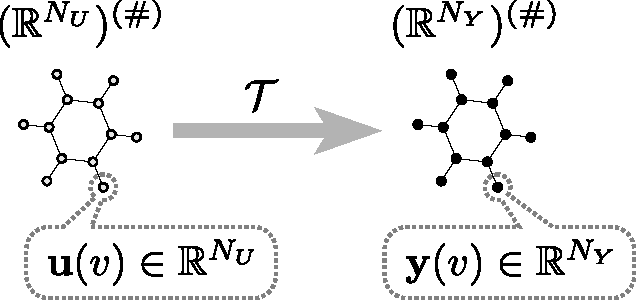
\includegraphics[width=0.5\columnwidth]{img/T-str2str}
\medskip
\caption{Trasduzione structure-to-structure.}
\label{fig:intro:trasduzione-s2s}
\end{figure}

\begin{figure}[tbp]
\centering
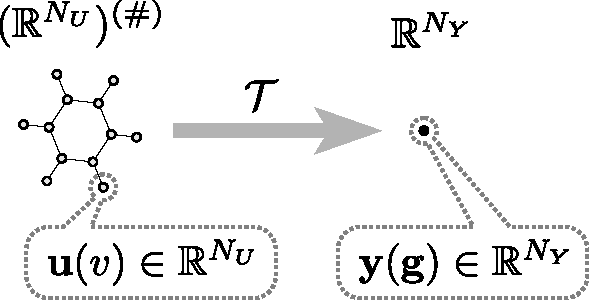
\includegraphics[width=0.5\columnwidth]{img/T-str2el}
\medskip
\caption{Trasduzione structure-to-element.}
\label{fig:intro:trasduzione-s2e}
\end{figure}

Nel caso dell'apprendimento supervisionato, l'allenamento avviene avvalendosi di un training-set $\mathfrak{T} = \setdef{(\graph{g}, \vect{y}_\textup{target}(g))}{\graph{g} \in \mathcal{G}, \vect{y}_\textup{target}(\graph{g}) \in (\R^{N_Y})^{\#}}$, dove $\vect{y}_\textup{target}(\graph{g})$ indica il target associato ad uno specifico input e può essere un grafo etichettato (isomorfo a $\graph{g}$) nel caso di trasduzioni structure-to-structure o un vettore di reali a dimensione fissa nel caso di trasduzioni structure-to-element.


%%%%%%%%%%%%%%%%%%%%%%%%%%%%%%%%%%%%%%%%%%%%%%%%%%%%%%%%%%%%%%%%%%%
\subsection{Graph Echo State Networks}\label{sec:intro:struct:gesn}
Le \emph{Graph Echo State Network} (GraphESN) \cite{Gallicchio:GraphESN} rappresentano un'estensione delle ESN (si veda il paragrafo~\ref{sec:intro:rc:esn}) --- e delle TreeESN \cite{Gallicchio:TreeESN} --- per il trattamento del dominio dei grafi.

In maniera simile ad una ESN, in una GraphESN sono distinguibili tre layer: uno di \emph{input}, uno nascosto detto \emph{reservoir} e formato da unità ricorsive e non lineari ed infine un \emph{readout} feedforward. Anche in questo caso è richiesto che la funzione di transizione di stato del reservoir sia contrattiva. Il reservoir viene dunque inizializzato affinché rispetti tale vincolo e rimane poi inalterato, mentre il solo readout viene allenato.\\
\`E importante sottolineare come la contrattività della funzione di transizione di stato assuma in questo caso un significato specifico di grossa rilevanza, ampliando la classe delle strutture supportate dal modello. La contrattività garantisce infatti la stabilità del processo di codifica anche nel caso di dipendenze cicliche fra le variabili di stato (si veda il paragrafo~\ref{sec:intro:struct}), determinando l'applicabilità del modello ad una classe di strutture che comprende grafi non diretti e/o ciclici.

Passiamo ora a caratterizzare più formalmente una GraphESN come modello per l'apprendimento di trasduzioni strutturali su un dominio di grafi.

Riprendendo quanto descritto in precedenza (si veda il paragrafo~\ref{sec:intro:struct:terminologia}), una trasduzione strutturale (\ref{eq:transduction}) può essere efficacemente decomposta come 
\begin{equation}\label{eq:intro:gesn:trasd}
\mathcal{T} = \mathcal{T}_\textup{out} \circ \mathcal{T}_\textup{enc}
\end{equation} 
dove $\mathcal{T}_\textup{enc} : (\R^{N_U})^{\#} \rightarrow (\R^{N_R})^{\#}$ è una \emph{funzione di encoding}, che mappa l'input in un dominio strutturato di features, e $\mathcal{T}_\textup{out} : (\R^{N_R})^{\#} \rightarrow (\R^{N_Y})^{\#}$ la \emph{funzione di output}. 
La figura~\ref{fig:intro:T-enc-out} mostra la realizzazione di una generica trasduzione strutturale (structure-to-structure) attraverso la composizione di una funzione di encoding, $\mathcal{T}_\textup{enc}$, ed una funzione di output, $\mathcal{T}_\textup{out}$.
\begin{figure}[tbp]
\centering
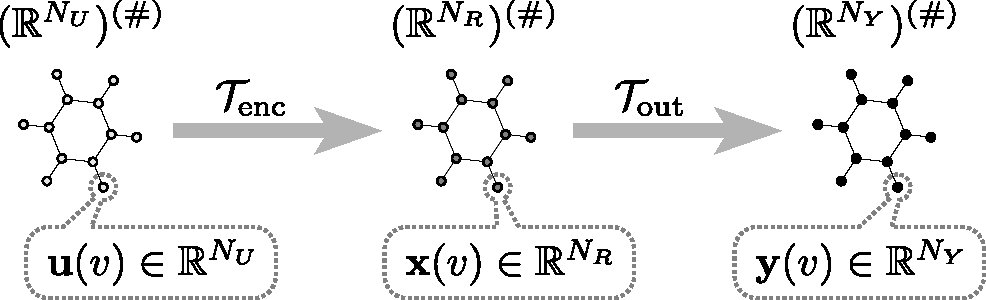
\includegraphics[width=0.8\columnwidth]{img/T-enc-out}
\medskip
\caption[Decomposizione di una trasduzione strutturale.]{Decomposizione di una trasduzione strutturale tramite una funzione di encoding $\mathcal{T}_\textup{enc}$ ed una funzione di output $\mathcal{T}_\textup{out}$.}
\label{fig:intro:T-enc-out}
\end{figure}

Secondo l'approccio neurale --- ricorsivo e ricorrente --- la funzione di encoding $\mathcal{T}_\textup{enc}$ viene realizzata da un sistema dinamico; lo spazio delle features $(\R^{N_R})^{\#}$ è composto da variabili di stato, associate ad ogni vertice dell'input. Chiamiamo $\vect{x}(v) \in \R^{N_R}$ l'informazione di stato associata al vertice $v$ del grafo in input $\graph{g}$. Indichiamo inoltre con $\vect{x}(\graph{g}) \in \R^{\abs{V(\graph{g})} N_R}$ la concatenazione degli stati associati a tutti i vertici dell'input, secondo un ordine arbitrario, e con $\vect{x}(\mathcal{N}(v)) \in \R^{\abs{\mathcal{N}(v)} N_R}$ la concatenazione degli stati associati ai vicini di un vertice $v$. La funzione $\mathcal{T}_\textup{enc}$ associa dunque ad ogni vertice dell'input $v \in V(\graph{g})$ una corrispondente informazione di stato secondo una \emph{funzione locale di encoding} $\tau$
\begin{equation}\label{eq:localenc}
\vect{x}(v) = \tau(\vect{u}(v), \mathcal{N}(v))
\end{equation}
che esprime la dipendenza dello stato associato al vertice $v$ da quelli associati ai suoi vicini. Equivalentemente possiamo dire che l'applicazione dell'equazione (\ref{eq:localenc}) ad ogni vertice dell'input realizza la \emph{funzione globale di encoding} $\hat{\tau}$
\begin{equation}\label{eq:globalenc}
\vect{x}(\graph{g}) = \hat{\tau}(\graph{g}, \vect{x}(\graph{g}))
\end{equation}
Dato un grafo in input $\graph{g}$, dunque, l'output della funzione di encoding $\mathcal{T}_\textup{enc}$ corrisponde alla soluzione dell'equazione (\ref{eq:globalenc}).

In una GraphESN la funzione $\mathcal{T}_\textup{enc}$ viene realizzata dal reservoir, che calcola iterativamente una \emph{funzione di transizione locale di stato}, versione iterativa dell'equazione (\ref{eq:localenc}). Al passo $t$, la funzione associa ad ogni vertice $v$ una codifica, o valore di stato, $\vect{x}_t(v)$ secondo la seguente equazione
\begin{equation}\label{intro:gesn:reservoir}
\vect{x}_t(v) 	= \tau( \vect{u}(v), \vect{x}_{t-1}(\mathcal{N}(v)) ) 
				= f( \matr{W}_{\textup{in}} \vect{u}(n) + \sum_{w \in \mathcal{N}(v)} \hat{\matr{W}} \vect{x}_{t-1}(w) )
\end{equation}
dove $\matr{W}_{\textup{in}} \in \R^{N_R \times (N_U + 1)}$ è la matrice dei pesi sulle connessioni tra input e reservoir, $\hat{\matr{W}} \in \R^{N_R \times N_R}$ è la matrice dei pesi ricorrenti tra i vicini di un vertice ed $f$ è la funzione di attivazione, tipicamente sigmoidale, delle unità del reservoir. La figura~\vref{fig:intro:encoding-step} mostra un passo del procedimento iterativo di encoding, evidenziando come lo stato calcolato per ogni vertice $v$ dipenda dall'etichetta numerica di input corrispondente, $\vect{u}(v)$, nonché dallo stato in corrispondenza dei vertici vicini calcolato al passo precedente, $\vect{x}(\mathcal{N}(v))$.

\begin{figure}[tbp]
\centering
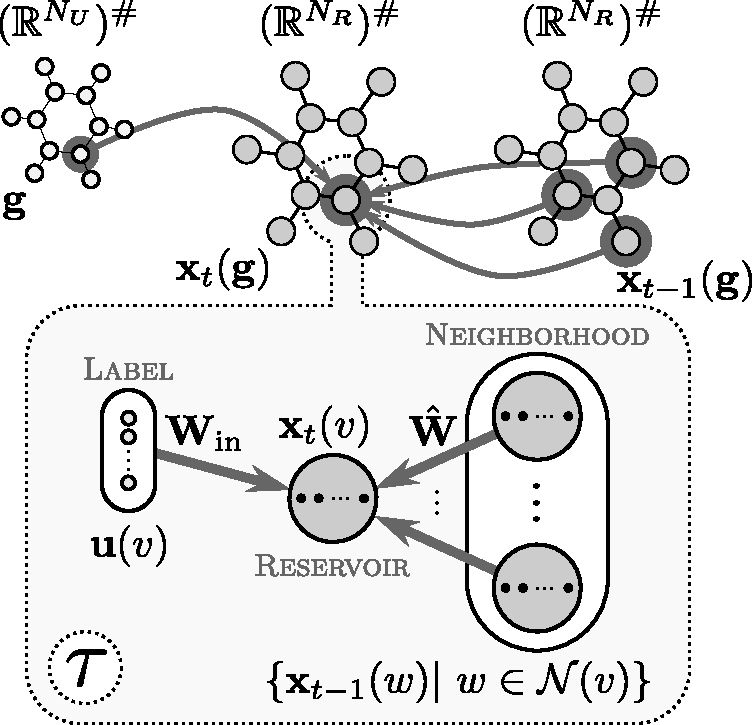
\includegraphics[width=0.6\columnwidth]{img/GraphESN-reservoir-application}
\medskip
\caption[Funzione di transizione locale di stato]{Schema di applicazione della funzione di transizione locale di stato ad un vertice $v$ dell'input $\graph{g}$.}
\label{fig:intro:encoding-step}
\end{figure}

Per poter garantire che l'encoding converga, e quindi che l'equazione (\ref{eq:globalenc}) abbia una soluzione, si ricorre ad un setting contrattivo della funzione $\tau$. Perché $\tau$ sia \emph{contrattiva} rispetto allo stato, è necessario che valga la seguente condizione:
\begin{multline}
\exists C \in [0,1) \mbox{ tale che } \forall \vect{u} \in \R^{N_U}, \forall \vect{x}_1, \dots , \vect{x}_k, \vect{x}'_1, \dots , \vect{x}'_k \in \R^{N_R} : \\
\vectnorm{\tau(\vect{u}, \vect{x}_1, \dots , \vect{x}_k) - \tau(\vect{u}, \vect{x}'_1, \dots , \vect{x}'_k)} \leq C \max_{i = 1, \dots ,k} \vectnorm{\vect{x}_i - \vect{x}'_i}
\end{multline}
dove $\vectnorm{\cdot}$ è una qualsiasi norma su $\R^{N_R}$. Considerando per $\tau$ l'implementazione dell'equazione~(\ref{intro:gesn:reservoir}), con $f=\tanh$ usata come funzione di attivazione delle unità del reservoir, e scegliendo la distanza euclidea come norma, risulta che la contrattività è garantita per \cite{Gallicchio:ExploitingVerticesStates}
\begin{equation}\label{eq:intro:gesn:sigma}
\sigma = \vectnorm{\hat{\matr{W}}}_2 k < 1
\end{equation}
dove $k$ è il grado massimo calcolato su tutti i grafi in $\mathcal{G}$ e $\sigma$, che controlla il grado di contrattività delle dinamiche del reservoir, è chiamato \emph{coefficiente di contrazione}. Una volta che la contrattività di $\tau$ sia assicurata, la convergenza del calcolo iterativo del reservoir è garantita dal \emph{Principio di Contrazione di Banach} \cite{Martelli:IntroductionToDiscrete} per ogni stato iniziale $\vect{x}_0(\graph{g})$; nella pratica questo permette di calcolare la codifica di un grafo in maniera iterativa, interrompendo l'elaborazione una volta che, per ogni vertice del grafo, la distanza tra due stati successivi nel processo di encoding sia inferiore ad una soglia prefissata $\epsilon$: $\vectnorm{\vect{x}_t(v) - \vect{x}_{t-1}(v)}_2 \leq \epsilon$. L'algoritmo~\vref{alg:intro:gesn:reservoir} mostra il processo di codifica ricorsivo implementato dal reservoir di una GraphESN.

\begin{algorithm}[tb]
\caption{GraphESN: algoritmo iterativo di encoding.}
\label{alg:intro:gesn:reservoir}
\begin{algorithmic}
\FORALL{$\graph{g} \in \mathcal{G}$}
	\STATE $t = 0$
	\FORALL{$v \in V(\graph{g})$}
		\STATE $\vect{x}_0(v) = 0$
	\ENDFOR
	\REPEAT
		\STATE $t = t+1$
		\FORALL{$v \in V(\graph{g})$}
			\STATE $\vect{x}_t(v) = \tau(\vect{u}(v), \vect{x}_{t-1}(\mathcal{N}(v)))$
		\ENDFOR
	\UNTIL{$\forall v \in V(\graph{g}) : \vectnorm{\vect{x}_t(v) - \vect{x}_{t-1}(v)}_2 \leq \epsilon$}
\ENDFOR
\RETURN $\vect{x}(\graph{g})$
\end{algorithmic}
\end{algorithm}

\`E opportuno sottolineare come la contrattività della funzione di transizione di stato caratterizza le GraphESN sotto diversi importanti aspetti, che vanno oltre quello algoritmico. Innanzi tutto la stabilità del processo di codifica rende le GraphESN in grado di gestire grafi ciclici, il che rappresenta invece un problema per le reti ricorrenti classiche. Inoltre la contrattività implica la echo state property (si veda il paragrafo~\ref{sec:intro:rc:esn}), garantendo che gli stati calcolati dal reservoir dipendano (asintoticamente) unicamente dal grafo in input e non dallo stato iniziale. Infine il fatto che $\tau$ sia contrattiva determina, come nel caso delle ESN, una caratterizzazione Markoviana delle dinamiche del reservoir, con il concetto di \emph{suffisso comune} esteso, rispetto al caso di sequenze \cite{Gallicchio:ArchitecturalAndMarkovian} o alberi \cite{Gallicchio:TreeESN}, al concetto di \emph{vicinato comune} \cite{Gallicchio:GraphESN}. 
\begin{figure}[tbp]
\centering
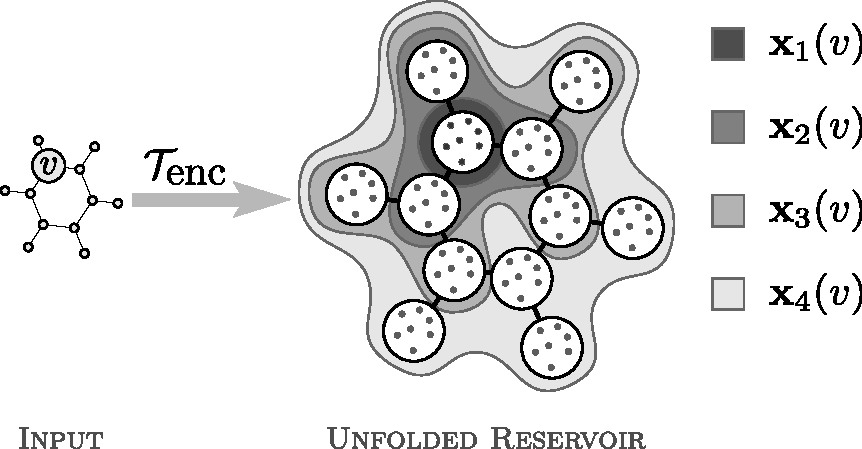
\includegraphics[width=0.7\columnwidth]{img/encoding-v2}
\medskip
\caption[Encoding di una GraphESN.]{Vertici coinvolti nel calcolo di $\vect{x}_t(v)$ durante quattro passi del processo di encoding.}
\label{fig:intro:encoding}
\end{figure}
La figura~\vref{fig:intro:encoding} mostra quali siano i vertici che contribuiscono al calcolo dello stato corrispondente ad un vertice $v$, evidenziando come nel corso di ogni iterazione la ``frontiera'' dei vertici coinvolti si allarghi. \`E bene sottolineare come, nella sua schematizzazione, la figura non renda conto del fatto che uno stesso vertice possa contribuire al calcolo dello stato di $v$ sia direttamente (i.e.\ il vertice appartiene a $\mathcal{N}(v)$) sia in maniera indiretta (i.e.\ per ogni cammino che partendo da $v$ si estenda, vicino dopo vicino ed iterazione dopo iterazione, fino al vertice in questione).

Nel caso di trasduzioni structure-to-element (si veda il paragrafo~\ref{sec:intro:struct:terminologia}) si ricorre ad un'ulteriore funzione $\mathcal{X} : (\R^{N_R})^{\#} \rightarrow \R^{N_R}$, detta \emph{state mapping function}, che applicata al risultato dell'encoding nello spazio strutturato di features restituisce una rappresentazione in uno spazio vettoriale a dimensione fissa per l'intero grafo. In questo caso l'equazione~(\ref{eq:intro:gesn:trasd}) viene dunque decomposta in
\begin{equation}
\mathcal{T} = \mathcal{T}_\textup{out} \circ \mathcal{X} \circ \mathcal{T}_\textup{enc}
\end{equation}
come mostrato dalla figura~\vref{fig:intro:T-enc-X-out}.
\begin{figure}[tbp]
\centering
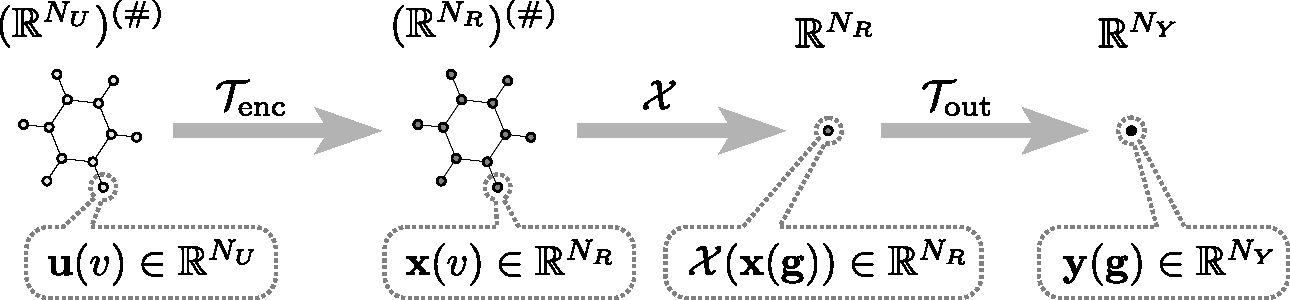
\includegraphics[width=\columnwidth]{img/T-enc-X-out}
\medskip
\caption[Decomposizione di una trasduzione structure-to-element.]{Decomposizione di una trasduzione structure-to-element tramite una funzione di encoding $\mathcal{T}_\textup{enc}$, una state-mapping-function $\mathcal{X}$ ed una funzione di output $\mathcal{T}_\textup{out}$.}
\label{fig:intro:T-enc-X-out}
\end{figure}

Benché la scelta della funzione $\mathcal{X}$ sia arbitraria, si distinguono principalmente due alternative. Con \emph{supersource state mapping} \cite{Gallicchio:TreeESN}, lo stato dell'intero grafo $\mathcal{X}(\vect{x}(\graph{g}))$ viene mappato nello stato di un solo vertice \emph{supersource}, qualora per la natura dei dati o del problema sia individuabile un vertice che dipenda da tutti gli altri\footnote{Questa caratteristica, naturale nel caso di alberi radicati e sequenze, è comunque realizzabile ``artificialmente'' per qualsiasi grafo aggiungendo un vertice che sia collegato a tutti gli altri.}. In alternativa, con \emph{mean state mapping}, $\mathcal{X}(\vect{x}(\graph{g}))$ viene calcolato come la media degli stati corrispondenti ai vertici di $\graph{g}$:
\begin{equation}\label{eq:meanstate}
\mathcal{X}(\vect{x}(\graph{g})) = \dfrac{1}{\abs{V(\graph{g})}} \sum_{v \in V(\graph{g})} \vect{x}(v)
\end{equation}

Come in una ESN, la funzione di output $\mathcal{T}_\textup{out}$ è realizzata da un \emph{readout} formato da $N_Y$ unità che ricevono input dal reservoir (o dalla state mapping function). \\
Nel caso di trasduzioni structure-to-structure, la \emph{funzione di output locale} applicata agli stati corrispondenti ai singoli vertici è la seguente:
\begin{equation}
\vect{y}(v) = g_\textup{out}(\vect{x}(v)) = f_\textup{out}(\matr{W}_\textup{out} \vect{x}(v))
\end{equation}
dove $\vect{y}(v) \in \R^{N_Y}$ è il vettore dei valori di output per il vertice $v$, $\matr{W}_\textup{out} \in \R^{N_Y \times (N_R + 1)}$ è la matrice dei pesi delle connessioni tra reservoir e readout ed $f_\textup{out}$ è la funzione di attivazione delle unità di output, tipicamente lineare. L'applicazione di $g_\textup{out}$ all'encoding ottenuto per ogni vertice dell'input definisce il calcolo della funzione di output $\mathcal{T}_\textup{out}$.\\
Per trasduzioni structure-to-element, l'output a dimensione fissa relativo all'intero grafo, $\vect{y}(\graph{g}) \in \R^{N_Y}$, è invece ottenuto applicando la funzione di output locale al risultato della state mapping function: 
\begin{equation}
\vect{y}(\graph{g}) = g_\textup{out}(\mathcal{X}(\vect{x}(\graph{g})) = f_\textup{out}(\matr{W}_\textup{out} \mathcal{X}(\vect{x}(\graph{g})))
\end{equation}

In entrambi i casi, ed in maniera simile a quanto accade in una ESN standard, l'allenamento di una GraphESN prevede l'adattamento dei pesi della matrice $\matr{W}_\textup{out}$, realizzabile attraverso regressione lineare\footnote{Purché $f_\textup{out}$ sia invertibile, è possibile ricondurre $g_\textup{out}$ ad una combinazione lineare semplicemente modificando i valori target: $\vect{y}_\textup{target}' = f_\textup{out}^{-1}(\vect{y}_\textup{target})$.} sulla base dei valori di target $\vect{y}_\textup{target}(v)$, o $\vect{y}_\textup{target}(\graph{g})$ nel caso di trasduzioni structure-to-element. 

La possibilità di limitare l'apprendimento alla sola funzione di output $g_\textup{out}$ e la realizzazione dell'encoding sfruttando il setting contrattivo del reservoir caratterizzano positivamente le GraphESN dal punto di vista computazionale rispetto ad altri modelli neurali per il trattamento di domini strutturati.\\
Assumendo che il reservoir sia sparso, con $M$ connessioni in input per ogni unità, il costo computazionale di un passo del processo di encoding ha costo
\begin{equation}
O(\abs{V(\graph{g})}\ k\ N_R\ M)
\end{equation}
ed ha dunque una dipendenza lineare sia con il numero di vertici dell'input che con le dimensioni del reservoir. Tale costo risulta molto inferiore, ad esempio, rispetto al processo di encoding realizzato durante la fase di training delle GNN \cite{Scarselli:GNN}, che avviene attraverso centinaia o migliaia di iterazioni, ognuna corrispondente all'intero processo di codifica dell'input di una GraphESN. 
Il costo computazionale dell'encoding è confrontabile anche con metodi basati su kernel applicati al trattamento di grafi. Mantenendo l'assunzione che $k$ sia il grado massimo riscontrabile sul dataset, l'applicazione dell'\emph{optimal assignment kernel} e del \emph{expected match kernel} \cite{Frohlich:AssignmentKernels} risulta infatti avere costo rispettivamente cubico e quadratico rispetto al numero di vertici dell'input.\\
Il costo del trainig varia invece a seconda dell'algoritmo utilizzato, potendo comunque fare affidamento sull'impiego di algoritmi efficienti per l'allenamento di un unico layer di unità feedforward (si veda il paragrafo~\ref{intro:alg}).

La figura~\vref{fig:intro:gesn} riassume schematicamente la struttura ed il funzionamento complessivo di una GraphESN che modelli traduzioni structure-to-element. Procedendo da sinistra verso destra, un grafo in input $\graph{g}$ viene codificato dal reservoir, che lo mappa in uno spazio delle features strutturato. La figura mostra in questo caso l'unfolding del reservoir, che viene ``copiato'' su ogni vertice dell'input. La varie copie così ottenute sono collegate, tramite connessioni con pesi in $\hat{\matr{W}}$, in accordo alla topologia del grafo (i.e.\ in base ai vicini di ogni vertice). Successivamente l'encoding ottenuto viene trasformato, dalla state mapping function $\mathcal{X}$, in un vettore di features a dimensione fissa. Il risultato dell'applicazione della state mapping function viene infine usato come input del readout, unica componente adattiva del modello, ottenendo in output il vettore a dimensione fissa $\vect{y}(\graph{g})$. In alto a sinistra la figura mostra la dipendenza che lega gli stati nello spazio delle features, sia all'etichetta di input del vertice corrispondente che agli stati calcolati in corrispondenza dei suoi vicini (i.e.\ un unico vicino nella figura).

\begin{figure}[tbp]
\centering
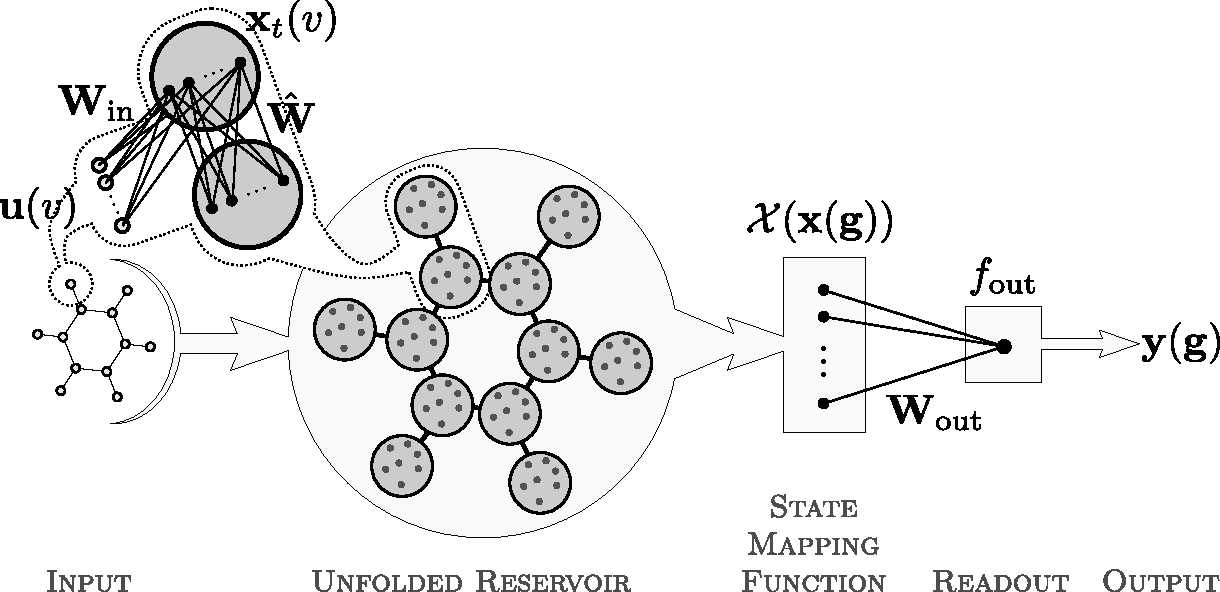
\includegraphics[width=0.95\columnwidth]{img/GraphESN-v2}
\medskip
\caption[GraphESN.]{Schema di una GraphESN per l'apprendimento di trasduzioni structure-to-element.}
\label{fig:intro:gesn}
\end{figure}


 \chapter{Modelli}\label{ch:modelli}
Il capitolo descrive i modelli realizzati, definendone sia le caratteristiche strutturali e topologiche che quelle computazionali.

Il paragrafo~\ref{sec:modelli:intro} fornisce un'introduzione ai modelli proposti, definendone i principi di base in relazione a quanto descritto nel capitolo~\ref{ch:background}.

Il paragrafo~\ref{sec:modelli:constr} introduce e discute i dettagli dell'estensione delle Graph\-ESN al caso costruttivo.

Nel paragrafo~\ref{sec:modelli:modelli} vengono descritti nello specifico i modelli oggetto della sperimentazione svolta, definendone le caratteristiche strutturali.

Nel paragrafo~\ref{sec:modelli:costo}, viene presentata un'analisi del costo computazionale relativo all'uso dei modelli proposti.

Infine, il paragrafo~\ref{ch:modelli:software} descrive le caratteristiche basilari dell'implementazione software dei modelli.

%%%%%%%%%%%%%%%%%%%%%%%%%%%%%%%%%%%%%%%%%%%%%%%%%%%%%%%%%%%%%%%

\section{Introduzione ai modelli}\label{sec:modelli:intro}
Tecniche, paradigmi e modelli descritti nel capitolo~\ref{ch:background}, benché appartenenti a periodi ed ambiti diversi, contribuiscono a formare i tratti distintivi dei modelli che saranno discussi nel corso del capitolo. Nel seguito saranno infatti introdotti dei modelli neurali, appartenenti all'ambito del Reservoir Computing, che adottino una strategia costruttiva nel trattamento di dati strutturati.

I modelli realizzati sono stati concepiti secondo un approccio incrementale, mirato ad introdurre e poi sfruttare l'approccio costruttivo con l'obiettivo di proporre soluzioni ad alcuni problemi aperti nell'ambito del Reservoir Computing. 
Ognuno dei modelli individua dunque nuove funzionalità specifiche, generalizzando i precedenti.

\begin{enumerate}[(i)]
\item Il modello \emph{GraphESN Constructive Flat} (GraphESN-CF) introduce una strategia costruttiva usando le GraphESN come unità computazionali. L'approccio costruttivo permette al modello di affrontare la necessità di fissare la topologia della rete a priori, particolarmente importante nel caso del Reservoir Computing data la presenza di reservoir non adattivi. Attraverso un procedimento iterativo di costruzione della rete, le GraphESN-CF sono dunque in grado di determinare il numero di unità da impiegare in maniera automatica e dipendente dal task: le singole sotto-reti vengono allenate per apprendere, e correggere, il segnale di errore commesso dalla rete, specializzandosi dunque ognuna in un sotto-task specifico, e vengono aggiunte alla rete in modo da formare una topologia \emph{flat}, che non preveda connessioni fra sotto-reti distinte.

\item Il modello \emph{GraphESN Forward} (GraphESN-FW) estende il precedente in modo da sfruttare le informazioni apprese nel corso del processo di costruzione incrementale della rete. Riprendendo la strategia della Cascade Correlation (si veda il paragrafo~\ref{sec:intro:cnn:ccorr}), in questo caso vengono aggiunte delle connessioni (in avanti, o \emph{forward}) fra l'output di ogni sotto-rete verso i readout di tutte le sotto-reti seguenti: quanto appreso da ogni sotto-rete contribuisce dunque alle fasi di learning successive, con lo scopo di semplificare la risoluzione del sotto-task affrontato. Grazie al fatto che ogni sotto-rete realizza una trasformazione non lineare dell'input, la GraphESN-FOF introduce una rete con topologia multilayer non lineare nell'ambito del Reservoir Computing.

\item Il modello \emph{GraphESN Forward Output-Feedback} (GraphESN-FOF) generalizza i due modelli precedenti introducendo uno schema output-feedback capace influenzare le dinamiche del reservoir. L'approccio costruttivo è in questo caso sfruttato per realizzare una strategia mirata ad affrontare uno dei problemi caratteristici del Reservoir Computing: l'impiego di un processo di encoding prefissato, guidato dalle caratteristiche dell'input ma non da quelle del task affrontato.\\
La topologia in questo caso si sviluppa connettendo gli output di ogni sotto-rete sia al readout che ai reservoir delle successive. I segnali di output delle sotto-reti, ottenuti tramite apprendimento ed utilizzabili sia su dati di training che su dati di test, vengono quindi introdotti all'interno del processo di codifica degli input, che pur rimanendo non adattivo beneficia di informazioni supervisionate, legate dunque al task affrontato.
\end{enumerate}

Altri aspetti caratterizzano i tre modelli realizzati.
Come appartenenti all'ambito del Reservoir Computing, i modelli fanno affidamento su una fase di learning estremamente vantaggiosa dal punto di vista computazionale, che interessa solo una parte delle connessioni della rete (si veda il capitolo~\ref{sec:intro:rc}). 
Infine, essendo estensioni delle GraphESN, i modelli proposti risultano in grado di apprendere trasduzioni strutturali generiche, che abbiano come input anche grafi non diretti o grafi diretti che presentino dei cicli (si veda il paragrafo~\ref{sec:intro:struct:gesn}).

Nel seguito i modelli verranno descritti nel dettaglio, privilegiando laddove possibile la formulazione più generale, ovvero riferendosi principalmente a GraphESN-FOF, in modo da non rendere la trattazione ridondante. Eventuali differenze specifiche, prevalentemente riferite alla topologia della rete, verranno evidenziate dove necessario.



%\begin{comment}
%Tecniche, paradigmi e modelli descritti nel capitolo~\ref{ch:background}, benché appartenenti a periodi ed ambiti diversi, hanno permesso di far emergere necessità e soluzioni che caratterizzano, ad oggi, la classe dei modelli neurali per il trattamento di domini strutturati. L'adozione di tecniche di allenamento efficienti e la capacità di trattare una classe di input che comprenda i grafi, risultano infatti essere fattori di grande importanza nella realizzazione di modelli per il trattamento di domini complessi. L'introduzione di un modello di Reservoir Computing per il l'apprendimento di trasduzioni su grafi, GraphESN, rappresenta una soluzione in grado di soddisfare entrambi i vincoli, ma presenta tuttavia alcuni limiti, tipici del Reservoir Computing.
%
%
%% costo computazionale e dominio di input
%% GraphESN risolve tutto ma ha alcuni problemi tipici del RC
%% Reservoir prefissato: chi mi dice quanto grosso?
%% Reservoir non adattivo: servono output-feedback.
%% L'approccio costruttivo offre soluzioni
%% Cosa faccio io?
%% - Introduco l'approccio costuttivo (risolvo il problema del reservoir prefissato)
%% - Sfrutto le informazioni apprese (come per CC)
%% - Sfrutto le informazioni apprese per introdurre uno schema di putput-feedback
%% ci sono altri vantaggi, tipici dell'approccio costruttivo: sotto-task specifici, politica locale nell'adattamento (caching), circoscrivere il learning a sotto-reti più piccole (vantaggio computaz)
%
%Tecniche, paradigmi e modelli descritti nel capitolo~\ref{ch:background} hanno permesso di far emergere necessità e soluzioni che caratterizzano ad oggi la classe dei modelli neurali per il trattamento di domini strutturati. 
%
%Con l'estensione del paradigma del Reservoir Computing al trattamento dei domini strutturati, tramite le GraphESN, è stato possibile realizzare modelli in grado di apprendere trasduzioni strutturali su grafi attraverso procedimenti di apprendimento poco onerosi. Nonostante l'efficienza computazionale e la classe degli input trattabili siano due fattori molto importanti nell'ambito delle Reti Neurali Ricorsive, le GraphESN mantengono tuttavia inalterate alcune delle criticità tipiche del Reservoir Computing. In particolare, la necessità di adottare reservoir prefissati e non adattivi rappresenta un limite 
%
%Nel capitolo~\ref{ch:background} 
%
%
%Nel seguito saranno dunque introdotti dei nuovi modelli neurali, appartenenti all'ambito del Reservoir Computing, che permettano di adottare una strategia costruttiva nel trattamento di dati strutturati.
%I modelli sono stati concepiti secondo un approccio incrementale, mirato ad introdurre e poi sfruttare l'approccio costruttivo. Ad ognuna delle seguenti fasi corrisponde dunque un modello distinto, in grado tuttavia di generalizzare i precedenti:
%\begin{enumerate}[(i)]
%\item Inizialmente si è introdotto l'approccio incrementale nell'ambito del Reservoir Computing attraverso la realizzazione di un modello che, estendendo le GraphESN, fosse in grado di determinare in maniera automatica la topologia e la dimensione della rete. La strategia costruttiva è stata realizzata utilizzando più GraphESN distinte, aggiunte in maniera incrementale e non connesse fra loro.\\
%L'adozione di un approccio costruttivo ha permesso 
%\item Sfruttare le informazioni precedentemente apprese dalla rete per potenziare 
%\item Introdurre uno schema stabile di output-feedback
%\end{enumerate}
%nel seguito, per semplicità, 
%
%\end{comment}
%
%\begin{comment}
%
%La formulazione e lo sviluppo dei modelli segue un approccio incrementale:
%- introduzione dell'approccio incrementale: flat
%- sfruttare informazioni già apprese per migliorare l'apprendimento
%- sfruttare le informazioni già apprese per realizzare un meccanismo di output-feedback.
%
%Da quanto detto emergono dunque necessità e limitazioni legate all'apprendimento di trasduzioni strutturali attraverso il paradigma neurale.
%In una disciplina fortemente orientata alle applicazioni come il Machine Learning, il costo computazionale e la classe degli input trattabili rappresentano infatti degli aspetti molto rilevanti. Il paradigma del Reservoir Computing offre soluzioni efficaci per rispondere a simili necessità, ma presenta tuttavia degli elementi critici. In particolare la presenza di una porzione di rete fissata a priori, e mantenuta inalterata durante l'apprendimento, si configura come una limitazione. La determinazione della topologia di rete appropriata e l'opportunità di modificare le dinamiche dell'intera rete sulla base del problema affrontato, sono infatti limiti la cui risoluzione rimane ad oggi un problema aperto \cite{Lukosevicius:ESNwithTrainedFeedbacks,Wyffels:stableOutputFeedback,Reinhart:ReservoirRegularization}.
%L'approccio costruttivo offre tuttavia soluzioni in tal senso, proponendo una strategia efficiente per determinare la topologia della rete in maniera automatica e per sfruttare le informazioni raccolte nel corso del processo incrementale di costruzione della rete.
%
%Nel seguito verranno introdotti dei nuovi modelli neurali, appartenenti all'ambito del Reservoir Computing, che permttano di adottare una strategia costruttiva nel trattamento di dati strutturati. 
%
%L'introduzione dell'approccio costruttivo, innovativo nell'ambito del Reservoir Computing, avviene in maniera incrementale, secondo tre fasi successive, che corrispondono ad altrettanti modelli.
%
%
%
%Tecniche, paradigmi e modelli descritti nel capitolo~\ref{ch:background}, benché appartenenti a periodi ed ambiti diversi, contribuiscono a formare i tratti distintivi dei modelli che saranno discussi nel corso del capitolo. Nel seguito saranno infatti introdotti dei modelli neurali, appartenenti all'ambito del Reservoir Computing, che permettano di adottare una strategia costruttiva nel trattamento di dati strutturati.
%
%Prima di introdurre i modelli originali, oggetto del lavoro svolto, è quindi possibile identificarne alcune caratteristiche di base, rifacendosi a quanto già descritto in precedenza, in modo da meglio comprenderne i tratti distintivi e, soprattutto, le motivazioni. 
%
%L'adozione di un approccio costruttivo, innovativo nell'ambito del Reservoir Computing, ha impatto sui modelli dal punto di vista computazionale ed algoritmico: permette la determinazione automatica della topologia della rete, la suddivisione di un task in più sotto-task, l'impiego di singole unità computazionali poco complesse e di algoritmi di apprendimento poco onerosi (si veda il paragrafo~\ref{sec:intro:cnn}). Applicata al caso del trattamento dei domini strutturati, inoltre, la strategia costruttiva offre l'opportunità di sfruttare localmente delle informazioni contestuali e supervisionate (si veda il paragrafo~\ref{sec:intro:struct}), tramite gli output-feedback, che possono essere utilizzate per influenzare le dinamiche del reservoir. 
%
%Come appartenenti all'ambito del Reservoir Computing, inoltre, i modelli sperimentati fanno affidamento su una fase di learning estremamente vantaggiosa dal punto di vista computazionale, che interessa solo una parte delle connessioni della rete (si veda il capitolo~\ref{sec:intro:rc}). 
%
%Infine, essendo estensioni delle GraphESN, i modelli proposti risultano in grado di apprendere trasduzioni strutturali generiche, che abbiano come input anche grafi non diretti o grafi diretti che presentino dei cicli (si veda il paragrafo~\ref{sec:intro:struct:gesn}).
%
%\end{comment}

%%%%%%%%%%%%%%%%%%%%%%%%%%%%%%%%%%%%%%%%%%%%%%%%%%%%%%%%%%%%%%%

\section{GraphESN costruttive}\label{sec:modelli:constr}
Stando anche a quanto descritto in precedenza (si veda il paragrafo~\vref{sec:intro:cnn}), l'approccio costruttivo prevede l'uso di singole unità computazionali, o sotto-reti, che interconnesse fra loro formano una rete nella sua totalità. Prima di poter descrivere i modelli sviluppati e definirne la topologia è dunque necessario dare una formulazione esatta di quali siano le unità di cui sono composti.

Come avviene in generale per i modelli costruttivi, consideriamo il caso in cui ogni nuova unità computazionale prenda in input gli output delle sotto-reti precedenti. Ogni sotto-rete agisce quindi come una sorta di feature-detector adattivo e la sua uscita può essere trattata come un input aggiuntivo dalle sotto-reti seguenti. Per far sì che più reti possano essere interconnesse fra loro, estendiamo reservoir e readout di una GraphESN standard in modo da rendere possibile la presenza di nuove connessioni (i.e.\ gli output di altre sotto-reti) che chiamiamo \emph{output-feedback}, provenienti da altre unità computazionali che operano indipendentemente da quella considerata.

Nel caso di trasduzioni structure-to-structure, gli output-feedback rappresentano valori calcolati in corrispondenza di ogni vertice. Il reservoir esteso della sotto-rete $i$-esima calcola, per un grafo in input $\graph{g}$ ed al passo $t$ del processo di codifica, un valore di stato $\vect{x}^{(i)}_t(v) \in \R^{N^{(i)}_R}$ per ogni vertice $v \in V(\graph{g})$ secondo la seguente equazione
\begin{equation}\label{eq:constructiveGESN:str2str}
\begin{split}	
\vect{x}^{(i)}_t(v)
	&= \tau( \vect{u}(v), \vect{x}^{(i)}_{t-1}(\mathcal{N}(v)), \vect{z}^{(1)}(v), \dots, \vect{z}^{(i-1)}(v) ) \\
	&= f( 
	\matr{W}^{(i)}_\textup{in} \, \vect{u}(v) + 
	\sum_{w \in \mathcal{N}(v)} \hat{\matr{W}}^{(i)} \, \vect{x}^{(i)}_{t-1}(w) +
	\sum_{j=1}^{i-1} \matr{W}^{(ij)}_\textup{fof} \, \vect{z}^{(j)}(v)
	)
\end{split}
\end{equation}
dove $\vect{z}^{(j)}(v) \in \R^{N^{(j)}_Z}$ rappresenta l'uscita della sotto-rete $j$-esima e $\matr{W}^{(ij)}_\textup{fof} \in \R^{N^{(i)}_R \times N^{(j)}_Z}$ è la matrice dei pesi per i (forward) output-feedback: connessioni tra il reservoir $i$-esimo e l'uscita della $j$-esima sotto-rete.

Nel caso di task structure-to-element cambia la natura degli output delle singole sotto-reti e l'equazione di transizione di stato del reservoir viene modificata di conseguenza come
\begin{equation}\label{eq:constructiveGESN:str2el}
\begin{split}	
\vect{x}^{(i)}_t(v) 
	&= \tau( \vect{u}(v), \vect{x}^{(i)}_{t-1}(\mathcal{N}(v)), \vect{z}^{(1)}(\graph{g}), \dots, \vect{z}^{(i-1)}(\graph{g}) ) \\
	&= f( 
	\matr{W}^{(i)}_\textup{in} \, \vect{u}(v) + 
	\sum_{w \in \mathcal{N}(v)} \hat{\matr{W}}^{(i)} \, \vect{x}^{(i)}_{t-1}(w) +
	\sum_{j=1}^{i-1} \matr{W}^{(ij)}_\textup{fof} \, \vect{z}^{(j)}(\graph{g})	
	)
\end{split}
\end{equation}
con $\vect{z}^{(j)}(\graph{g}) \in \R^{N^{(j)}_Z}$. 

Al netto della modifica effettuata, il processo di codifica dell'input da parte del reservoir rimane inalterato in entrambi i casi (si veda il paragrafo~\ref{sec:intro:struct:gesn} e l'algoritmo~\vref{alg:intro:gesn:reservoir}).

Il readout delle sotto-reti viene invece modificato considerando gli output-feedback come parte della codifica del grafo in input. In altri termini, la codifica viene arricchita da nuove informazioni o features che, calcolate dalle precedenti sotto-reti, vengono concatenate al vettore risultato del processo di encoding del reservoir.\\
Nel caso di trasduzioni structure-to-structure, l'uscita $\vect{z}^{(i)}(v) \in \R^{N^{(i)}_Z}$ della sotto-rete $i$-esima è quindi data da
\begin{equation}
\begin{split}
\vect{z}^{(i)}(v) 
	&= g_\textup{out}( \vect{x}^{(i)}(v), \vect{z}^{(1)}(v), \dots, \vect{z}^{(i-1)}(v) ) \\
	&= f_\textup{out}( \matr{W}^{(i)}_\textup{out} \, 
		[\vect{x}^{(i)}(v), \vect{z}^{(1)}(v), \dots, \vect{z}^{(i-1)}(v)] )
\end{split}
\end{equation}
con $[\vect{x}^{(i)}(v), \vect{z}^{(1)}(v), \dots, \vect{z}^{(i-1)}(v)]$ concatenazione della codifica corrispondente al vertice $v$ e degli output-feedback e con la matrice dei pesi del readout opportunamente modificata per adattarsi alla nuova dimensione dello spazio delle features, $\matr{W}^{(i)}_\textup{out} \in \R^{N^{(i)}_Z \times (N^{(i)}_R + \sum_{j = 1}^{i-1} N^{(j)}_Z + 1)}$.

Per le trasduzioni structure-to-element si procede in maniera simile, calcolando l'output relativo all'intero grafo $\vect{z}^{(i)}(\graph{g})$ come
\begin{equation}
\begin{split}
\vect{z}^{(i)}(\graph{g}) 
	&= g_\textup{out}( \mathcal{X}(\vect{x}^{(i)}(\graph{g})), \vect{z}^{(1)}(\graph{g}), \dots, \vect{z}^{(i-1)}(\graph{g}) ) \\
	&= f_\textup{out}( \matr{W}^{(i)}_\textup{out} \,
		[\mathcal{X}(\vect{x}^{(i)}(\graph{g})), \vect{z}^{(1)}(\graph{g}), \dots, \vect{z}^{(i-1)}(\graph{g})] )
\end{split}
\end{equation}

Poiché la natura del readout rimane sostanzialmente invariata rispetto al caso delle GraphESN, non sono necessari particolari accorgimenti per la fase di learning, che può essere eseguita con le tecniche standard.

\`E importante sottolineare alcuni aspetti relativi alla formulazione data delle singole unità computazionali.
\begin{itemize}
\item La presenza degli output-feedback è opzionale (e.g.\ $\matr{W}^{(ij)}_\textup{fof} = \vect{0}$). Questo fornisce la possibilità di implementare diverse varianti architetturali (si vedano i paragrafi~\ref{sec:modelli:constr:costruzione} e \ref{sec:modelli:modelli}) e permette di caratterizzare le singole unità computazionali come vere e proprie estensioni delle GraphESN standard. La presenza opzionale degli output-feedback determina anche il fatto che i tre modelli realizzati si generalizzino a vicenda, secondo la gerarchia descritta in precedenza nel paragrafo~\ref{sec:modelli:intro}.

\item Non è stato posto alcun vincolo particolare sulle caratteristiche di una singola unità computazionale in relazione al fatto che più sotto-reti debbano interagire fra loro. Benché ognuna sia predisposta per ricevere gli output-feedback dalle precedenti è dunque possibile che ciascuna sotto-rete differisca dalle altre nelle dimensioni del reservoir, del readout o dell'output. Questa caratteristica consente quindi l'impiego di sotto-reti eterogenee sia nelle dimensioni che nel sotto-task affrontato, permettendo la realizzazione di numerose varianti implementative.

\item I pesi dei singoli output-feedback sono tutti indipendenti l'uno dall'altro. Ne risulta un'ampia gamma di possibilità nell'implementare politiche di feedback specifiche, ad esempio facendo in modo che alcune sotto-reti abbiano maggiore influenza sulle altre (i.e.\ abbiano pesi maggiori sulle connessioni di output-feedback).

\item Gli output-feedback, agendo come input ausiliari, non modificano le condizioni per la contrattività del reservoir.
\end{itemize}
Nel seguito verrà descritto il funzionamento della rete nella sua totalità e sarà discusso in dettaglio il ruolo degli output-feedback.


%%%%%%%%%%%%%%%%%%%%%%%%%%%%%%%%%%
\subsection{Costruzione di una rete}\label{sec:modelli:constr:costruzione}
Dopo aver definito come sono fatte le singole unità che formano la rete nel suo complesso, è possibile indicare quale sia l'approccio usato per combinarle. 

Consideriamo una rete come formata da un \emph{readout globale} al quale vengono collegate in ingresso le connessioni corrispondenti alle uscite di una o più sotto-reti, aggiunte incrementalmente. Al passo $i$-esimo, ovvero dopo aver aggiunto $i$ sotto-reti, l'output della rete è dunque dato, nel caso di trasduzioni structure-to-structure, da:
\begin{equation}\label{eq:modelli:globalreadout-str2str}
\vect{y}^{(i)}(v) = f_\textup{out}( \matr{W}_\textup{out} \, [\vect{z}^{(1)}(v), \dots, \vect{z}^{(i)}(v)] )
\end{equation}
con $\matr{W}_\textup{out} \in \R^{N_Y \times (\sum_{j=1}^{i} N_Z^{(i)} + 1)}$ matrice dei pesi delle connessioni del readout globale. Nel caso dell'apprendimento di trasduzioni structure-to-element l'output è calcolato, in maniera simile, come
\begin{equation}\label{eq:modelli:globalreadout-str2el}
\vect{y}^{(i)}(\graph{g}) = f_\textup{out}( \matr{W}_\textup{out} \, [\vect{z}^{(1)}(\graph{g}), \dots, \vect{z}^{(i)}(\graph{g})] )
\end{equation}
In entrambi i casi siamo in presenza di un unico livello di connessioni che può essere allenato attraverso tecniche efficienti, in analogia con quanto avviene nelle sotto-reti ed in accordo con l'approccio del Reservoir Computing.

Internamente alla rete, ogni nuova sotto-rete può essere collegata a tutte le altre sotto-reti esistenti: gli output-feedback possono andare al reservoir della nuova sotto-rete, al suo readout o ad entrambi, in accordo con quanto descritto nel paragrafo~\ref{sec:modelli:constr}. Il modo in cui le sotto-reti sono connesse fra loro determina la differenza fra i modelli sperimentati, le cui topologie verranno descritte in seguito (si veda il paragrafo~\vref{sec:modelli:modelli}).

Ogni sotto-rete viene allenata per \emph{correggere l'errore} commesso dalla rete (i.e.\ dal readout globale). Riferendoci al caso di un task structure-to-element\footnote{Il passaggio al caso di task structure-to-structure è banale e viene quindi tralasciato per chiarezza espositiva.}, indichiamo con $\vect{e}^{(i)}(\graph{g}) \in \R^{N_Y}$ l'errore commesso dalla rete al passo $i$-esimo (i.e.\ dopo aver aggiunto $i$ sotto-reti) sull'input $\graph{g}$. La sotto-rete $(i+1)$-esima utilizza dunque $\vect{e}^{(i)}(\graph{g})$ come target nella propria fase di apprendimento. Una volta effettuato il training, la sotto-rete viene ``congelata'' ed aggiunta alla rete: il suo output diventa un nuovo input per il readout globale e può, eventualmente, essere usato come output-feedback per le sotto-reti successive. Ogni volta che una nuova unità computazionale allenata viene aggiunta alla rete si esegue un nuovo allenamento del readout globale, necessario a valutare se interrompere l'algoritmo o, in alternativa, a determinare i nuovi errori da correggere tramite ulteriori sotto-reti. 
L'allenamento del readout globale, il cui input ha una dimensionalità ridotta rispetto ai readout delle sotto-reti, ha tuttavia un costo computazionale contenuto.
L'algoritmo procede dunque iterativamente aggiungendo nuove sotto-reti e modificando l'errore, finché non venga verificato un criterio di stop prefissato (e.g.\ l'errore di training non scenda al di sotto di una soglia prefissata).

\begin{algorithm}[tb]
\caption{GraphESN costruttiva. Caso structure-to-element.}
\label{alg:modelli:constr}
\begin{algorithmic}
\STATE init sub-network counter: $i = 0$
\STATE init error: $\vect{e}^{(0)}(\graph{g}) = -\vect{y}_\textup{target}(\graph{g})$
\REPEAT
	\FORALL{$1 \leq j \leq pool\_size$}
		\STATE init $j$-th candidate
		\STATE connect candidate's output-feedback
		\STATE train candidate using $\vect{e}^{(i)}(\graph{g})$ as target 
	\ENDFOR
	\STATE select the winning candidate
	\STATE update sub-network counter: $i = i+1$
	\STATE connect the winner (i.e.\ $i$-th sub-network) to the global readout
	\STATE train the global readout
	\STATE update error $\vect{e}^{(i)}(\graph{g})$
\UNTIL{stop adding sub-networks}
\end{algorithmic}
\end{algorithm}

L'algoritmo~\vref{alg:modelli:constr} riassume il procedimento iterativo di costruzione della rete, mostrando anche come la fase di training delle sotto-reti possa avvalersi di un pool di candidate come avviene per la Cascade Correlation (si veda il paragrafo~\ref{sec:intro:cnn:ccorr}). In questo caso il pool di candidate può contenere sotto-reti che si differenziano, oltre che per l'esito dell'apprendimento, anche nell'iperparametrizzazione o nell'inizializzazione dei pesi, in particolare dei pesi del reservoir che non vengono modificati dal training.

Poiché al primo passo non è disponibile alcuna informazione sull'errore commesso, la prima sotto-rete viene allenata considerando l'errore massimo:  $\vect{e}^{(0)}(\graph{g}) = -\vect{y}_\textup{target}(\graph{g}), \forall \graph{g} \in \mathcal{G}$. Tale scelta risponde ad un'esigenza ben precisa. Il segnale appreso da una sotto-rete gioca infatti un ruolo ambivalente rispetto alla risoluzione del task: da una parte serve al readout globale come indicazione degli errori da correggere, dall'altra sposta gli stati delle sotto-reti successive in modo da raggruppare i pattern potenzialmente già corretti (si veda il paragrafo~\ref{sec:modelli:constr:outfeedback}). In quest'ottica è quindi importante che la prima sotto-rete agisca in maniera analoga alle successive, seppur riferendosi ad un errore per certi versi artificiale.

\`E infine opportuno sottolineare che la strategia incrementale adottata permette di allenare il readout globale attraverso metodi iterativi (e.g.\ LMS, si veda il paragrafo~\ref{intro:alg}). Tale pratica, comune nell'ambito delle Reti Neurali Artificiali, risulta infatti generalmente inapplicabile nel caso del Reservoir Computing a causa dell'alto numero di condizionamento delle matrici di input utilizzate per allenare quei readout che prendano i propri input direttamente da un reservoir \cite{Jaeger:ReservoirRiddles}, cosa che non avviene nel caso del readout globale, i cui input sono le uscite (precedentemente allenate) delle varie sotto-reti.



%%%%%%%%%%%%%%%%%%%%%%%%%%%%%%%%%%
\subsection{Output-feedback}\label{sec:modelli:constr:outfeedback}
Il ruolo degli output-feedback è di rilevanza centrale per i modelli proposti, in particolare rispetto al modo in cui questi possono influenzare le dinamiche del reservoir. Con riferimento al reservoir esteso dell'equazione~(\ref{eq:constructiveGESN:str2el}) è infatti importante sottolineare come i valori in $\vect{z}^{(j)}(\graph{g})$ introducano \emph{localmente} un'informazione \emph{globale}, riferita all'intero grafo in input\footnote{Nel caso di un task structure-to-structure, equazione~(\ref{eq:constructiveGESN:str2str}), è forse più corretto parlare di informazione \emph{contestuale} piuttosto che globale. Tale differenza nella terminologia è tuttavia irrilevante ai fini del discorso affrontato se non addirittura fuorviante se si considera che il processo di encoding di una GraphESN sfrutta di per sé informazioni contestuali, anche se di natura diversa da quelle qui riferite.}, e \emph{supervisionata}, ottenuta cioè tramite il processo di apprendimento (i.e.\ gli output-feedback corrispondono agli output di altre sotto-reti, precedentemente allenate). Se per la sua natura Markoviana un reservoir ha la capacità di discriminare i vertici in base ai loro vicini (ed i vicini dei vicini, e così via, iterativamente), il reservoir esteso usufruisce quindi, sia in training che in test, anche di un'informazione che gli permette di ``vedere oltre'' la frontiera che determina lo stato corrente (si veda la figura~\ref{fig:intro:encoding}) ed in base a questo di spostare gli stati in maniera consistente con il task affrontato, in funzione del target.

L'idea di sfruttare le caratteristiche dell'output per influenzare le dinamiche del reservoir è d'altra parte presente nell'ambito del Reservoir Computing sin dalla nascita delle ESN \cite{Jaeger:EchoStateApproach} e risponde all'esigenza di superare i limiti imposti dall'adozione di reservoir fissi, con dinamiche prefissate. Nonostante questo, ad oggi l'impiego di output-feedback nella loro formulazione originale comporta tecniche ed accorgimenti specifici \cite{Lukosevicius:ESNwithTrainedFeedbacks, Wyffels:stableOutputFeedback, Prokhorov:AppealAndChallenges} e presenta alcune limitazioni (si veda il paragrafo~\ref{sec:intro:rc:esn}).
I modelli proposti introducono dunque, in contrapposizione con i modelli esistenti di Reservoir Computing, un sistema di output-feedback stabile realizzato sfruttando le caratterstiche della strategia costruttiva.

Per comprenderne meglio la natura, la figura~\ref{fig:modelli:aux} mostra un esempio di come gli output-feedback possano modificare le dinamiche della rete. 
\begin{figure}[tb]
\centering
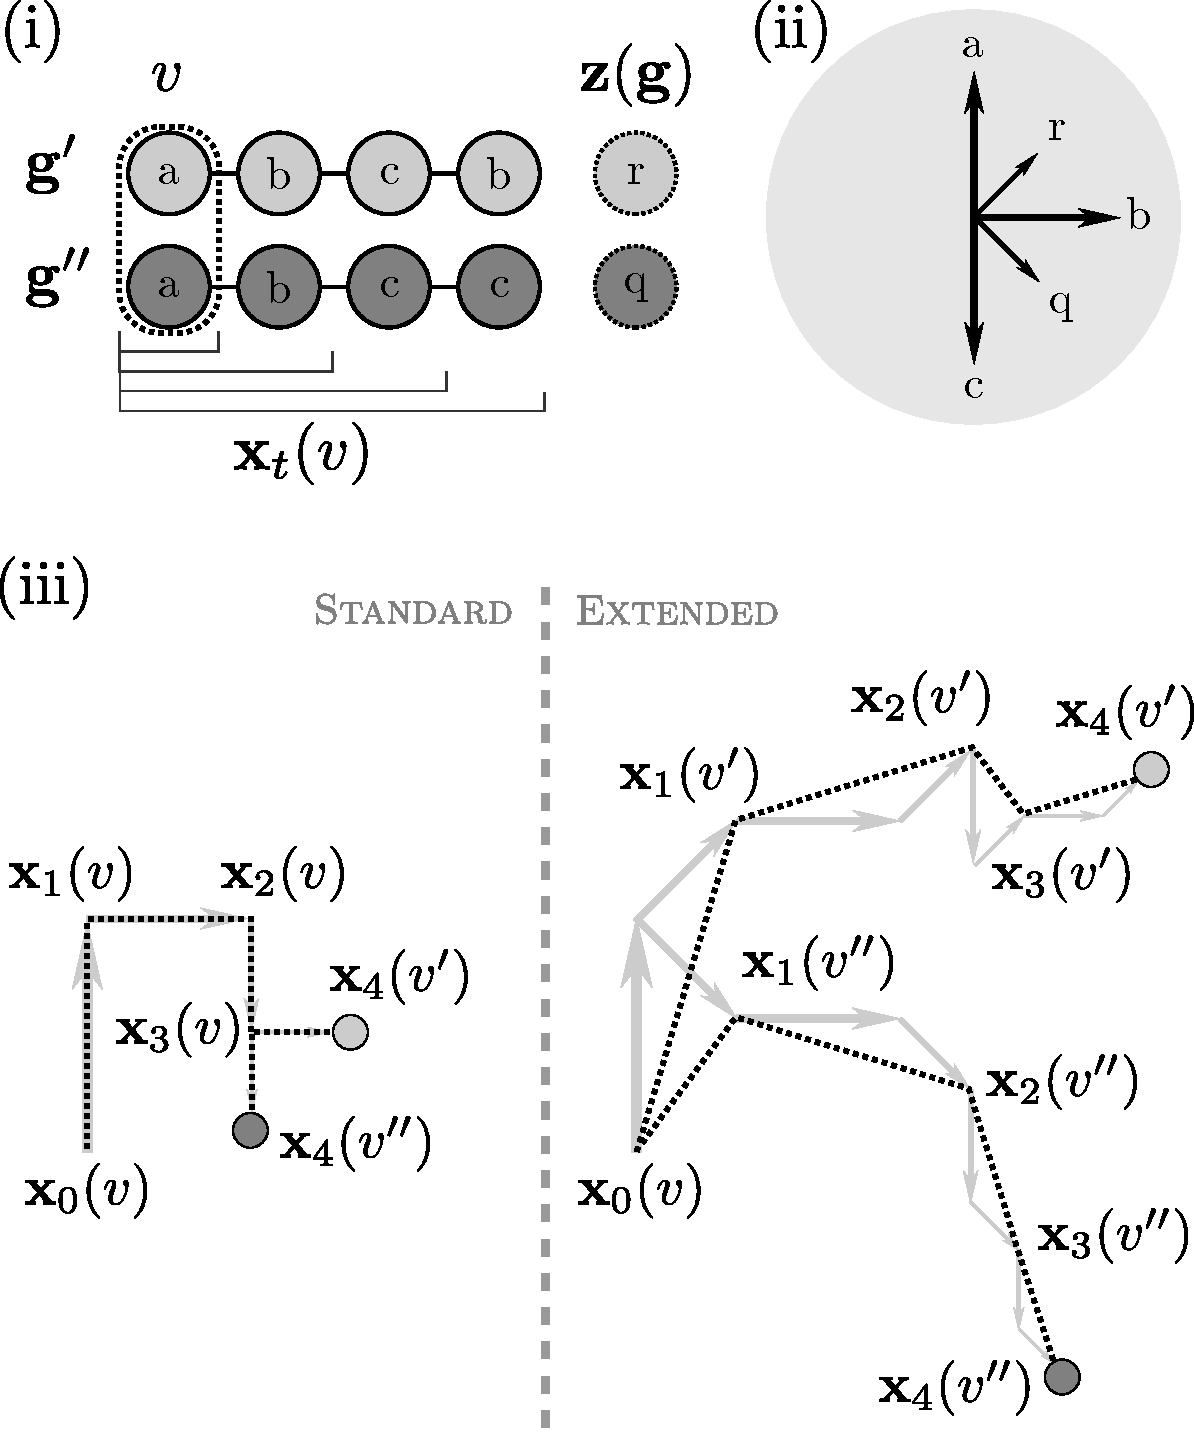
\includegraphics[width=0.65\columnwidth]{img/spazio-stati}
\medskip
\caption[Dinamiche del Reservoir esteso.]{Effetto degli output-feedback sul reservoir esteso: esempio di encoding in uno spazio bidimensionale.\\(i) Input; (ii) interpretazione geometrica degli input; (iii) traiettorie nel feature space, (\emph{sx}) reservoir standard, (\emph{dx}) reservoir esteso.}
\label{fig:modelli:aux}
\end{figure}
Con riferimento alla figura, si considerino (i) due sequenze in input $\graph{g}'$ e $\graph{g}''$, a cui siano associati target diversi (i.e.\ che debbano essere distinte dalla rete), che differiscono unicamente nell'ultimo vertice ed a cui sono associati valori di output-feedback distinti, indicati con $r$ e $q$ rispettivamente. Supponendo che lo spazio delle feature sia bidimensionale (i.e.\ $N_R = 2$), è possibile dare un'interpretazione geometrica ai vari input (e.g.\ $\matr{W}_\textup{in}\, \mathrm{a} = (0,1)$), che supponiamo essere come è indicato in (ii). In (iii) sono mostrate le traiettorie corrispondenti all'encoding iterativo del primo vertice della sequenza, indicato con $v'$ e $v''$ rispettivamente per i due input o semplicemente con $v$ quando le traiettorie nello spazio degli stati coincidono per entrambi i casi. \\
Nel caso di un un reservoir standard, a sinistra nella figura, i due input seguono la stessa traiettoria per le prime tre iterazioni. Le due sequenze sono dunque indistinguibili fino al quarto passo, ovvero fino a quando l'insieme dei vertici che determina lo stato $\vect{x}(v)$ è sufficientemente ampio da includere l'ultimo vertice. Si nota inoltre come, per effetto della natura Markoviana del reservoir, gli spostamenti delle variabili di stato si riducano con l'aumentare delle iterazioni di modo che l'ultima iterazione, quella determinante per discriminare $\graph{g}'$ e $\graph{g}''$ nel reservoir standard, mantenga comunque le due codifiche $\vect{x}_4(v')$ e $\vect{x}_4(v'')$ molto vicine nello spazio degli stati. \\
Sulla destra sono invece mostrate le traiettorie nel caso in cui ai due input sia associato un output-feedback differente, tenuto in considerazione dal reservoir esteso nel corso del processo di encoding. La figura evidenzia come in questo caso le traiettorie si differenzino sin dalla prima iterazione, permettendo di discriminare le due sequenze ben prima che l'encoding di $v'$ e $v''$ arrivi ad includere l'etichetta dell'ultimo vertice e con l'effetto di portare $\vect{x}_4(v')$ e $\vect{x}_4(v'')$ in punti molto più lontani all'interno del feature space rispetto a quanto avverrebbe con un reservoir standard.

Per effetto dello spostamento appena descritto, dunque, i pattern in input tenderanno a raggrupparsi nello spazio degli stati in maniera consistente con i propri valori degli output-feedback. \`E importante notare che, quando le varie sotto-reti sono allenate per riprodurre un segnale legato all'errore residuo commesso dalla rete (e.g.\ emulando l'errore o massimizzando la correlazione fra il proprio output e l'errore, si veda il paragrafo~\vref{sec:intro:cnn:ccorr}), allora si avrà uno spostamento maggiore in quegli input per cui sia stato precedentemente riconosciuto un alto errore residuo, e che hanno dunque maggiore probabilità di essere stati corretti dalla rete nei passi precedenti (si veda anche il paragrafo~\ref{sec:modelli:constr:costruzione}). Informalmente potremmo dire che gli output-feedback, provenienti da altre unità computazionali, hanno in questo caso l'effetto di ``mettere da parte'' gli input i cui errori siano già stati corretti da altre sotto-reti, permettendo dunque al learning di concentrarsi maggiormente su una porzione di pattern per i quali la rete commette gli errori maggiori.



%%%%%%%%%%%%%%%%%%%%%%%%%%%%%%%%%%
\section{Modelli}\label{sec:modelli:modelli}
Come detto in precedenza, i modelli sperimentati si distinguono nel modo in cui le varie sotto-reti vengono collegate fra loro. 

Mantenendo il denominatore comune dell'approccio costruttivo, secondo i principi e le modalità già descritte, i tre modelli proposti si inseriscono in un percorso incrementale che guarda all'arricchimento della struttura nelle connessioni in modo da sfruttare l'introduzione di informazione supervisionata attraverso la presenza degli output-feedback. 


\subsubsection*{GraphESN-CF}
Il modello \emph{GraphESN-CF} (i.e.\ GraphESN Constructive Flat) rappresenta l'estensione delle GraphESN al caso costruttivo: le singole sotto-reti vengono aggiunte incrementalmente ma non vi è alcuna connessione fra i loro output. Il modello è quindi formato da un unico strato di sotto-reti e dal readout globale, senza che sia presente alcun output-feedback.

La figura~\vref{fig:modelli:cf} mostra schematicamente la topologia del modello GraphESN-CF.
\begin{figure}[tb]
\centering
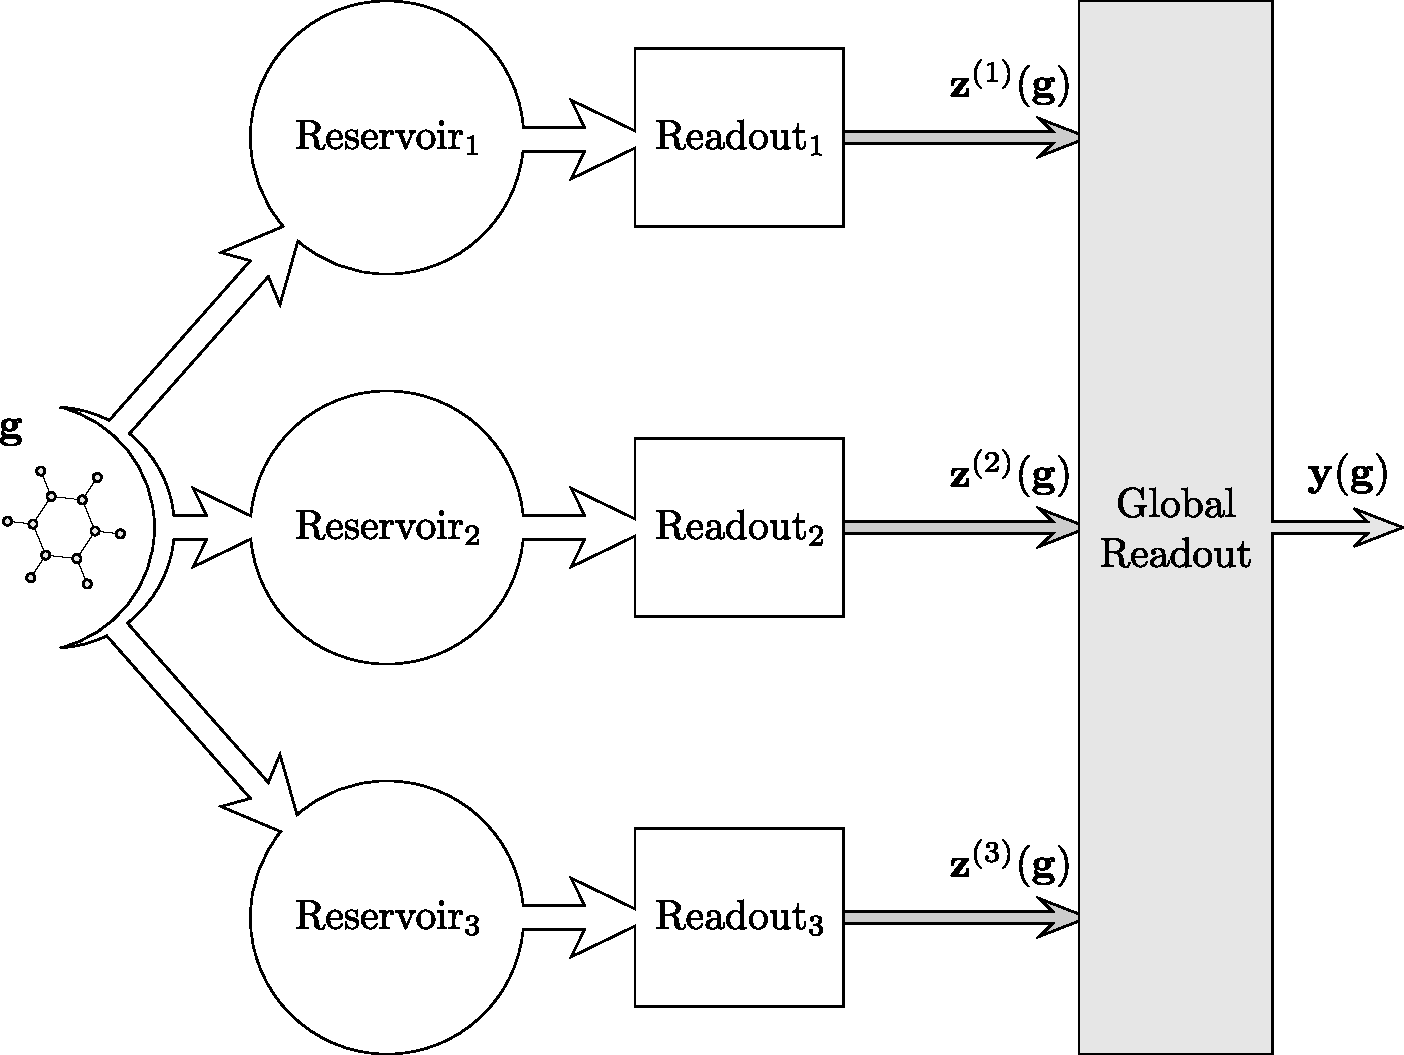
\includegraphics[width=0.8\columnwidth]{img/Modello-CF}
\medskip
\caption[GraphESN-CF.]{Modello GraphESN-CF. Topologia con tre sotto-reti.}
\label{fig:modelli:cf}
\end{figure}


\subsubsection*{GraphESN-FW}
Il modello \emph{GraphESN-FW} (i.e.\ GraphESN Forward) arricchisce il precedente attraverso una struttura più complessa. In questo caso, infatti, il readout di ogni sotto-rete riceve in input gli output-feedback provenienti dalle sotto-reti precedenti. Il risultato è una struttura in cascata in cui, in maniera simile a quanto accade per la Cascade Correlation (si veda il paragrafo~\ref{sec:intro:cnn:ccorr}), ogni sotto-rete forma un livello a sé stante dipendente dai precedenti. Poiché gli output-feedback vanno da una sotto-rete a tutte le successive, le connessioni si sviluppano ``in avanti''.

La figura~\vref{fig:modelli:fw} mostra la topologia del modello GraphESN-FW, con le connessioni in avanti.

Alcune osservazioni sono opportune riguardo alla presenza di output-feedback ed alla particolare scelta di una struttura a cascata in avanti. L'esistenza di output-feedback, infatti, determina implicitamente una relazione di dipendenza fra le varie unità computazionali (i.e.\ per poter svolgere la propria elaborazione, ogni sotto-rete necessita dell'output delle sotto-reti dalle quali riceve output-feedback). La struttura a cascata in avanti individua dunque un ordinamento parziale che mette il modello nelle condizioni di poter funzionare, determinando anche una strategia di esecuzione specifica (i.e.\ gli output vengono calcolati in sequenza, a partire dalla prima sotto-rete in poi).\\
Il fatto che gli output-feedback siano solo in avanti ha anche il vantaggio di mantenere inalterate tutte quelle sotto-reti per cui siano già state svolte delle elaborazioni, con l'effetto pratico di poter salvare i risultati ottenuti (e.g.\ l'encoding dei singoli input da parte dei reservoir) e risparmiare dunque risorse di calcolo.

\begin{figure}[p]
\centering
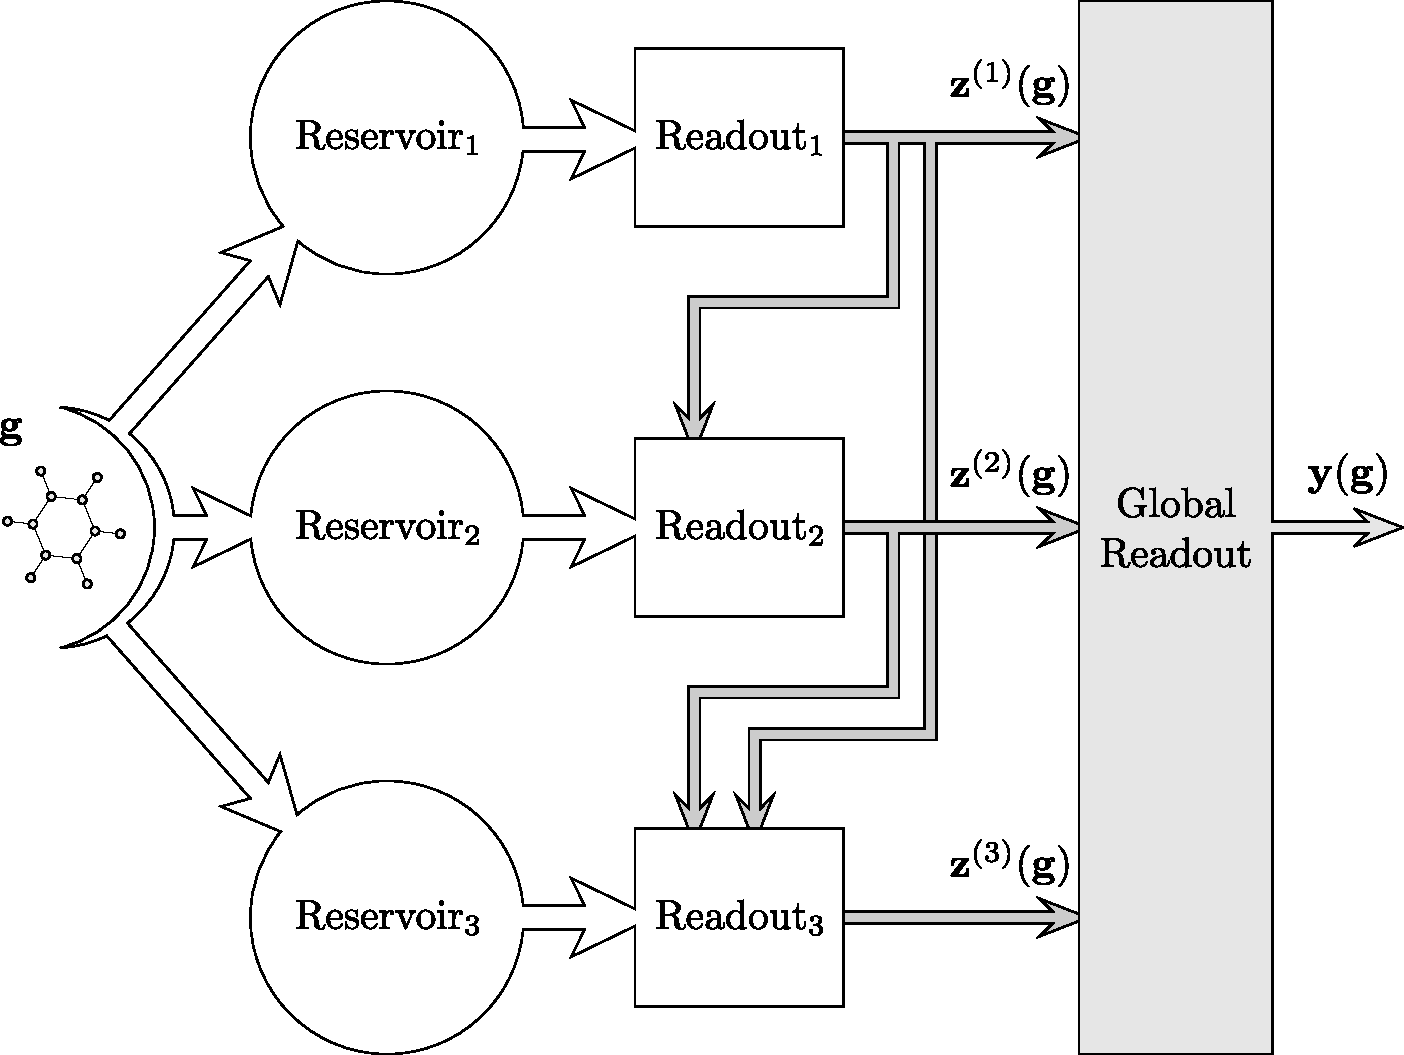
\includegraphics[width=0.8\columnwidth]{img/Modello-FW}
\medskip
\caption[GraphESN-FW.]{Modello GraphESN-FW. Topologia con tre sotto-reti.}
\label{fig:modelli:fw}
\end{figure}

\begin{figure}[p]
\centering
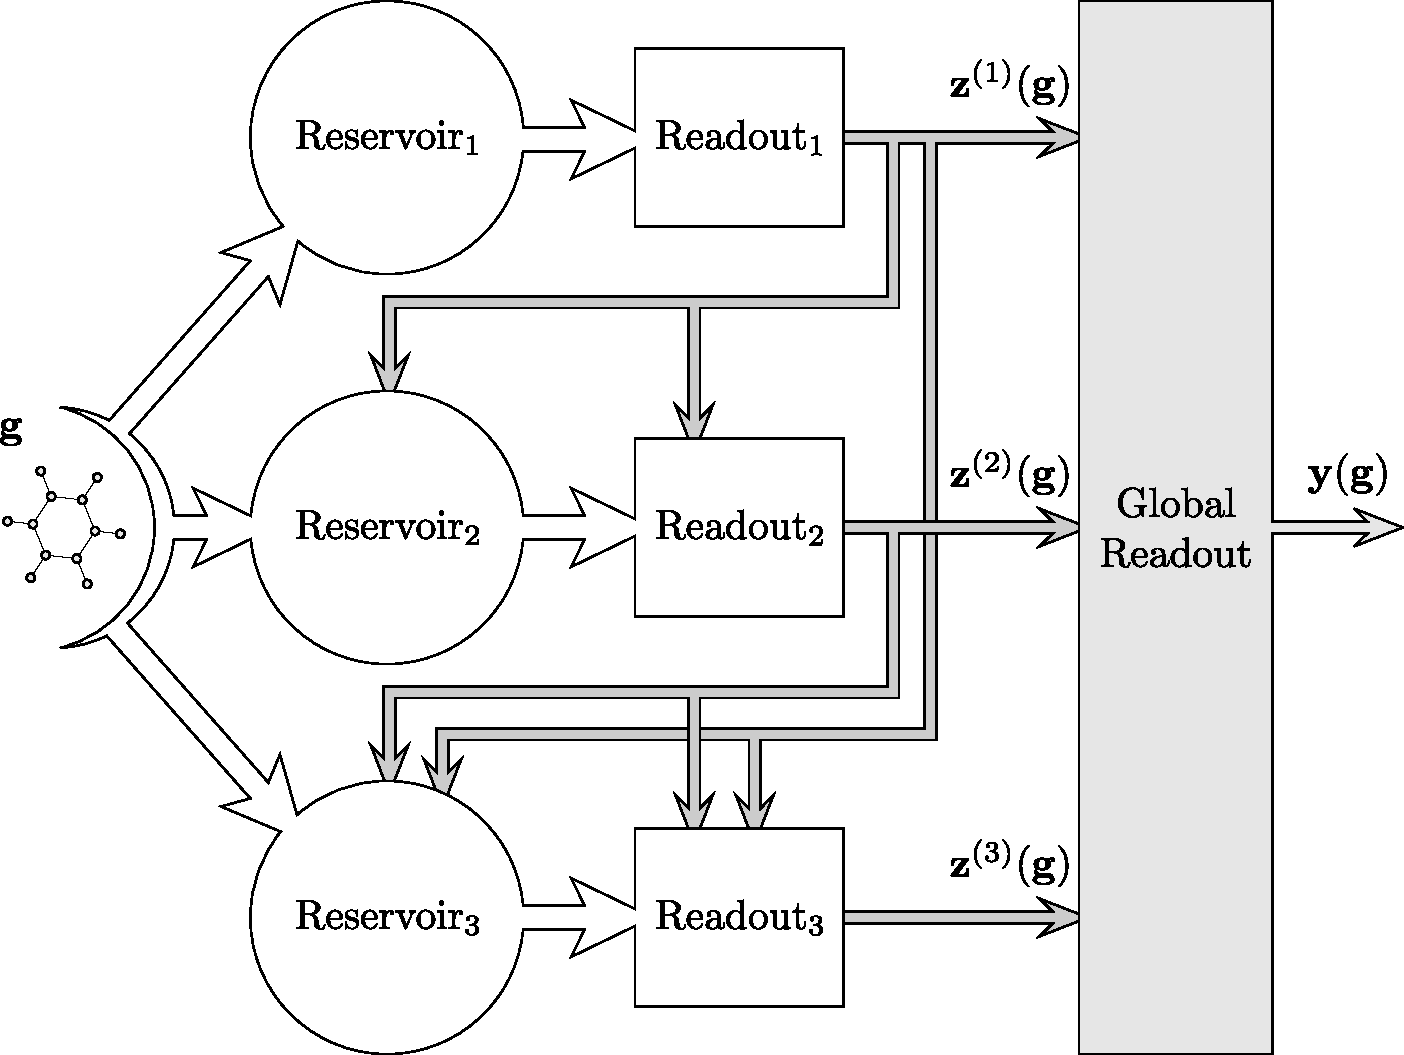
\includegraphics[width=0.8\columnwidth]{img/Modello-FOF}
\medskip
\caption[GraphESN-FOF.]{Modello GraphESN-FOF. Topologia con tre sotto-reti.}
\label{fig:modelli:fof}
\end{figure}

\subsubsection*{GraphESN-FOF}
L'ultimo modello proposto, \emph{GraphESN-FOF} (i.e.\ Graph\-ESN Forward Output-Feedback), e combina l'approccio incrementale, la struttura a cascata in avanti e l'uso degli output-feedback per spostare gli stati del reservoir come discusso nel paragrafo~\ref{sec:modelli:constr:outfeedback}. In questo caso, dunque, le connessioni in avanti sono mandate sia al readout che al reservoir di tutte le sotto-reti successive.

La struttura delle connessioni del modello GraphESN-FOF è mostrata nella figura~\ref{fig:modelli:fof}. La figura~\vref{fig:modelli:evoluzione} mostra invece i primi tre passi del processo incrementale di costruzione di una rete.


\begin{figure}[p]
\centering
\subfloat[][Struttura della rete dopo una iterazione.]
{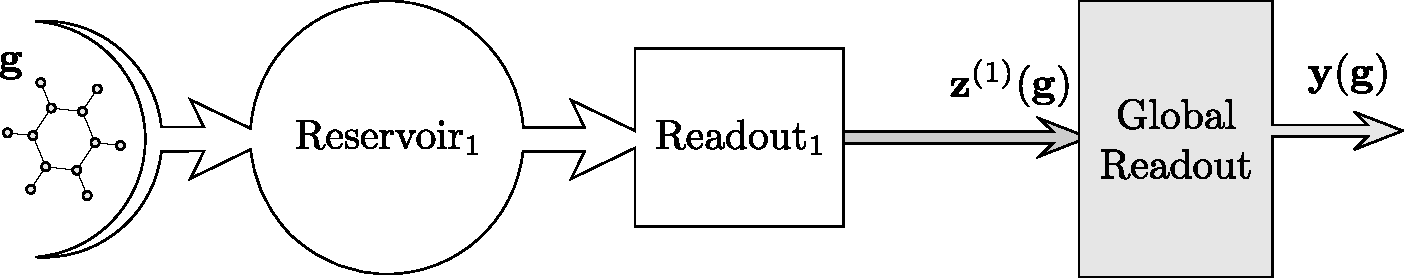
\includegraphics[width=0.75\columnwidth]{img/evoluzione1}}\\
\vspace*{0.4cm}
\subfloat[][Struttura della rete dopo due iterazioni.]
{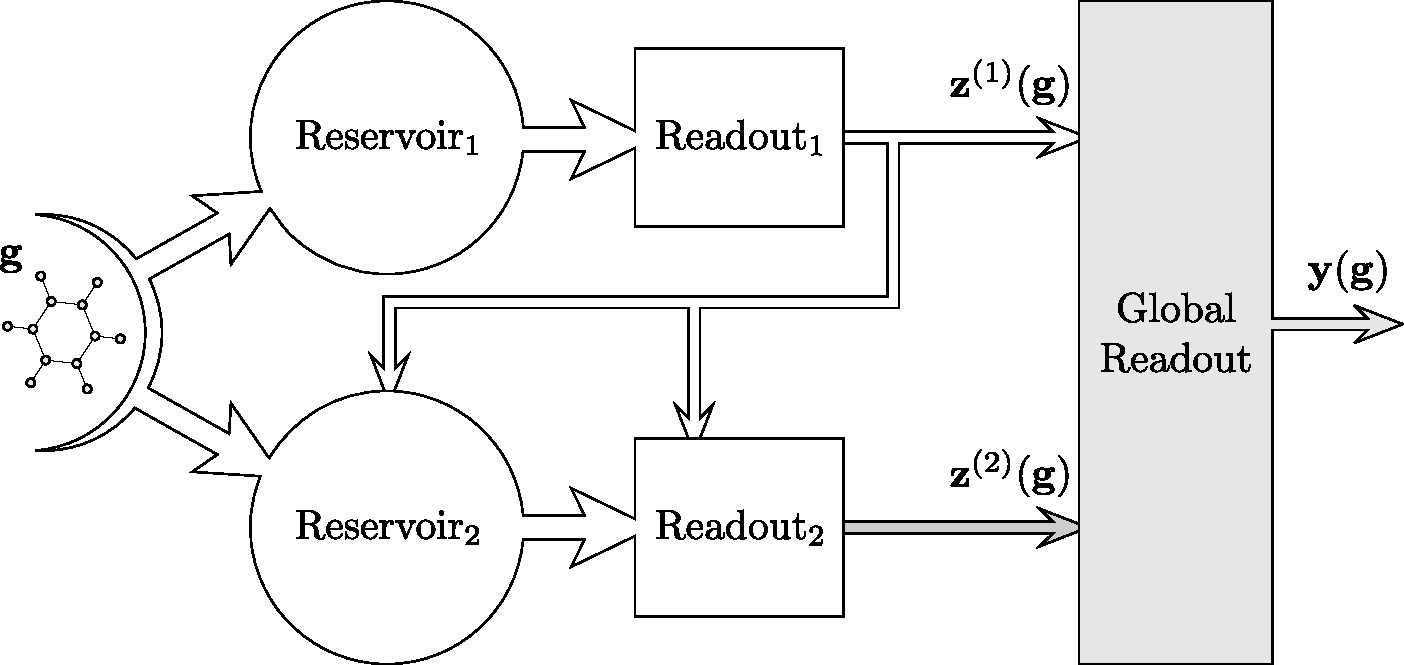
\includegraphics[width=0.75\columnwidth]{img/evoluzione2}}\\
\vspace*{0.4cm}
\subfloat[][Struttura della rete dopo tre iterazioni.]
{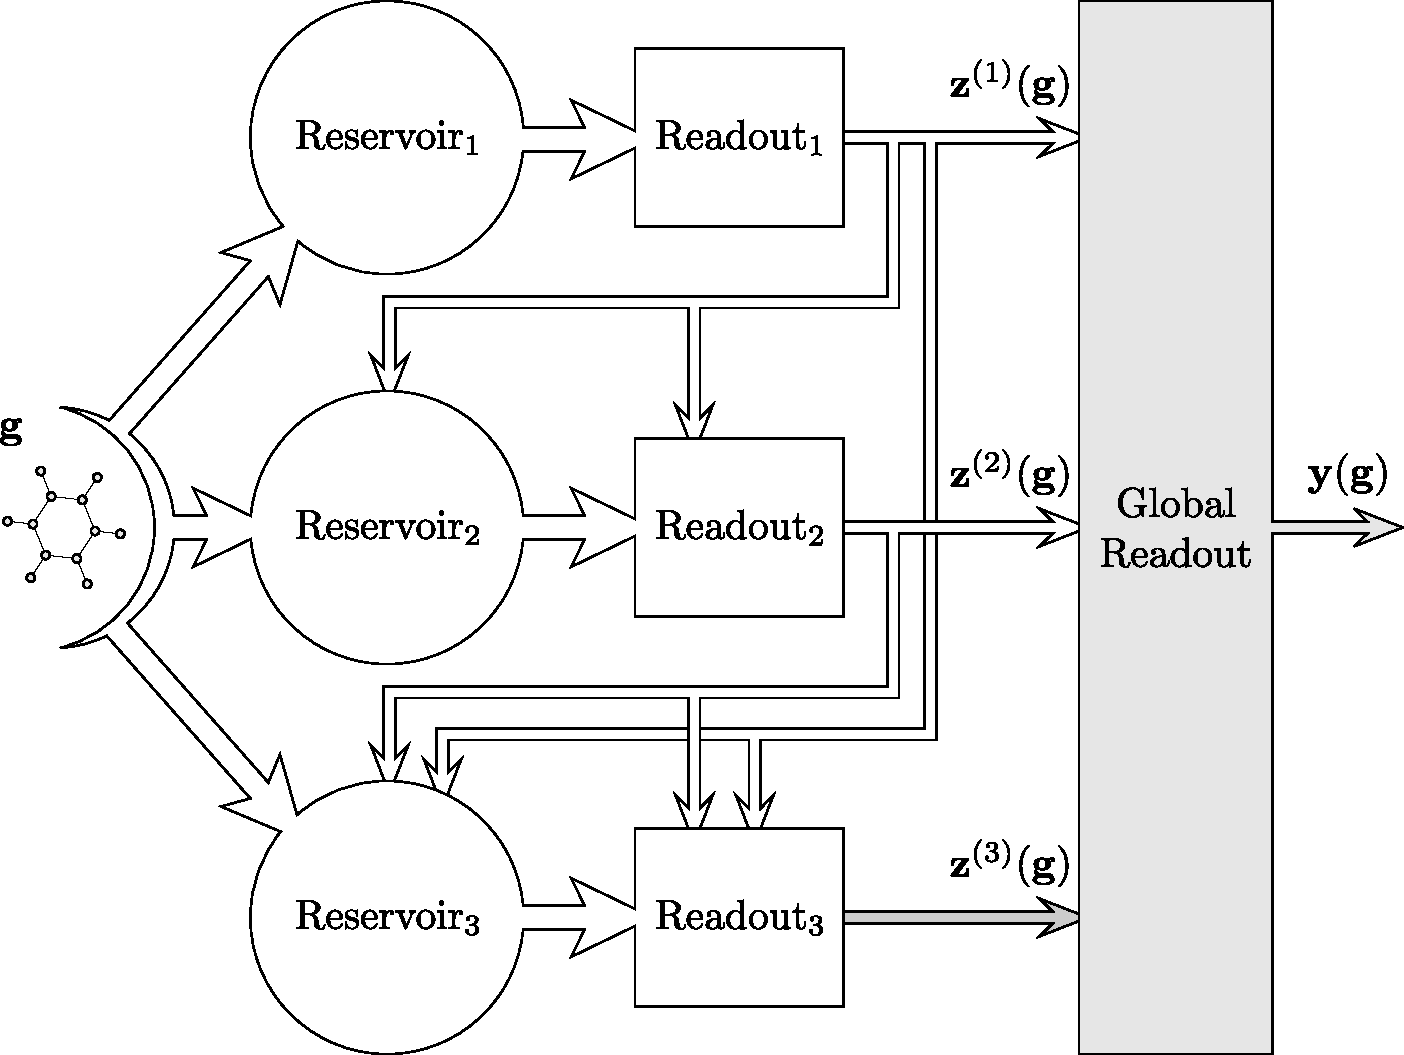
\includegraphics[width=0.75\columnwidth]{img/evoluzione3}}
\vspace*{0.4cm}
\medskip
\caption[Costruzione di una rete.]{Costruzione di una rete di tipo GraphESN-FOF. Dall'alto verso il basso, tre passi successivi di costruzione della rete. Ad ogni iterazione sono mostrate in grigio le connessioni soggette ad allenamento.}
\label{fig:modelli:evoluzione}
\end{figure}


%%%%%%%%%%%%%%%%%%%%%%%%%%%%%%%%%%
\section{Costo computazionale}\label{sec:modelli:costo}
Consideriamo una rete di tipo GraphESN-FOF formata da $\mathit{NSN}$ sotto-reti, ognuna con $N_R$ unità nel reservoir. Assumiamo inoltre, secondo un'ipotesi tutt'altro che irrealistica, che la dimensione dell'output della rete e delle sotto-reti sia trascurabile (tipicamente $N_Y = N_Z = 1$). Di seguito viene riportato il costo computazionale delle fasi principali che caratterizzano l'evoluzione della rete (si veda l'algoritmo~\vref{alg:modelli:constr}). Il dettaglio del calcolo del costo computazionale è riportato nell'appendice~\ref{app:costo}.

\subsubsection*{Encoding}
Ogni sotto-rete deve far convergere il proprio reservoir per ogni input $\graph{g} \in \mathcal{G}$ e quindi ottenere l'encoding corrispondente nello spazio delle features. Grazie alle caratteristiche dei modelli sperimentati è sufficiente che ogni sotto-rete esegua questa fase una sola volta per ogni input. 

Chiamando $\mathit{MAXV}$ il numero massimo di vertici di un grafo del dataset $\mathcal{G}$ (i.e.\ $\mathit{MAXV} = \max(\{ \abs{V(\graph{g})},\, \graph{g} \in \mathcal{G} \})$) e $\mathit{MAXIT}$ il numero massimo di iterazioni consentite per la convergenza di un singolo reservoir, il costo computazionale complessivo del processo di encoding risulta essere
\begin{equation}
	O( \mathit{NSN}\ \mathit{MAXIT}\ \mathit{MAXV}\ \abs{\mathcal{G}}\ N_R^2 )
\end{equation}
Il costo totale della codifica degli input scala quindi quadraticamente rispetto alle dimensioni del reservoir. \`E opportuno tuttavia osservare che, nel caso dei modelli proposti, la possibilità di scomporre il task in sotto-task permette l'adozione di sotto-reti di dimensioni contenute.
\\
Come nel caso delle GraphESN standard questa fase è identica sia per gli input usati nel training della rete che per il test.

Benché negli esperimenti riportati nel seguito (capitolo~\ref{ch:esperimenti}) siano stati utilizzati reservoir completamente connessi, sfruttando la presenza di sotto-reti di dimensioni contenute, il costo computazionale dell'encoding può essere ridotto assumendo una connettività sparsa nel reservoir. Nel caso in cui ogni unità del abbia al più $M$ connessioni in ingresso, il costo dell'encoding diventa
\begin{equation}
	O( \mathit{NSN}\ \mathit{MAXIT}\ \mathit{MAXV}\ \abs{\mathcal{G}}\ N_R\ M )
\end{equation}
e dipende dunque linearmente dalla dimensione dell'input e dei reservoir utilizzati.

La fase di encoding realizzata tramite i modelli proposti si caratterizza dunque, come nel caso delle GraphESN (si veda anche il paragrafo~\ref{sec:intro:struct:gesn}), per efficienza computazionale se confrontata con altri modelli per il trattamento di domini strutturati. 
Particolarmente interessante può essere in questo caso il confronto con tecniche basate su kernel: l'uso di kernel su grafi \cite{Frohlich:AssignmentKernels} comporta infatti un costo almeno quadratico rispetto al numero di vertici dell'input, e realizza un encoding non adattivo, secondo metriche prefissate. Con i modelli introdotti risulta invece possibile, ad un costo computazionale vantaggioso, realizzare la codifica dell'input tenendo conto anche dell'informazione supervisionata derivante dagli output-feedback.

I dettagli del calcolo per il costo computazionale dell'encoding sono riportati nel paragrafo~\ref{app:costo:encoding}.

\subsubsection*{Training}
Distinguiamo due distinte fasi di training, in accordo con la strategia costruttiva descritta in precedenza: il training di una singola sotto-rete e l'allenamento del readout-globale. Poiché il training riguarda in ogni caso l'adattamento dei pesi di un unico livello di connessioni, verso il readout, vari algoritmi possono essere efficacemente applicati. Nel seguito saranno considerate solo le strategie utilizzate nell'analisi sperimentale dei modelli.

Una sotto-rete può essere allenata per emulare l'errore commesso dal readout-globale. In questo caso, ricorrendo all'algoritmo di Ridge Regression (si veda il paragrafo~\ref{intro:alg}) il costo computazionale complessivo è 
\begin{multline}
	O( \mathit{NSN}^4 + N_R\ \mathit{NSN}^3 + N_R^2\ \mathit{NSN}^2 + N_R^3\ \mathit{NSN} \\ 
	+ \mathit{NSN}^3\ \abs{\mathcal{G}} + \mathit{NSN}^2\ N_R\ \abs{\mathcal{G}} + \mathit{NSN}\ N_R^2\ \abs{\mathcal{G}} )
\end{multline}
e scala dunque con il numero di sotto-reti elevato alla quarta e con il cubo della dimensione del reservoir, secondo una dipendenza critica nel determinare il vantaggio computazionale, come verrà discusso nel seguito.

Il readout-globale della rete può a sua volta essere allenato tramite Ridge Regression, con un costo complessivo
\begin{equation}
	O( \mathit{NSN}^4 + \mathit{NSN}^3 \abs{\mathcal{G}} )
\end{equation}
\`E tuttavia possibile allenare il readout-globale con Least Mean Squares (si veda il paragrafo~\ref{intro:alg}). Sia $\mathit{LMSIT}$ il numero massimo di iterazioni necessarie alla convergenza dell'algoritmo, il costo complessivo è 
\begin{equation}
	O( \mathit{LMSIT}\ \abs{\mathcal{G}}\ \mathit{NSN}^2\ )
\end{equation}
In questo caso la dipendenza è quadratica rispetto al numero complessivo di sotto-reti.

Il calcolo completo del costo computazionale dell'allenamento delle sotto-reti tramite Ridge Regression è riportato nel paragrafo~\ref{app:costo:tr_sub}, mentre i paragrafi~\ref{app:costo:tr_globale_ridge} e \ref{app:costo:tr_globale_lms} riportano il calcolo del costo per l'allenamento del readout globale tramite Ridge Regression e LMS rispettivamente.

\subsubsection*{Calcolo dell'output}
Ogni volta che una nuova sotto-rete viene allenata ed aggiunta alla rete è necessario procedere con il calcolo dell'output relativo ad ognuno dei grafi nel dataset $\mathcal{G}$. Nell'intero processo di costruzione della rete il costo del calcolo dell'output, a livello delle sotto-reti, risulta 
\begin{equation}
	O(\mathit{NSN}\ N_R\ \abs{\mathcal{G}} + \mathit{NSN}^2\ \abs{\mathcal{G}})
\end{equation}
presentando una dipendenza quadratica rispetto al numero di sotto-reti e lineare rispetto alla dimensione del dataset e del reservoir.
\`E opportuno in questo caso sottolineare come, per una generica sotto-rete, il calcolo dell'uscita dipenda dagli output-feedback delle sotto-reti precedenti, i cui valori sono precalcolati, e dal risultato della fase di encoding, anch'esso già calcolato durante la fase di allenamento.

Ad ogni incremento delle dimensioni della rete è inoltre necessario ottenere l'errore commesso dal readout-globale e quindi calcolare l'output della rete. Poiché il readout-globale prende in input unicamente gli output delle singole sotto-reti il costo complessivo è
\begin{equation}
	O(\mathit{NSN}^2\ \abs{\mathcal{G}})
\end{equation}
e scala linearmente con la dimensione del dataset e quadraticamente rispetto al numero di sotto-reti.

Il dettaglio del calcolo del costo computazionale per ottenere l'output delle sotto-reti e del readout globale è riportato nei paragrafi~\ref{app:costo:out_sub} e \ref{app:costo:out_globale} rispettivamente.

\subsubsection*{Costo complessivo}
In riferimento ad una GraphESN-FOF, con reservoir completamente connesso, che usi l'algoritmo Ridge Regression per l'apprendimento, è  possibile riassumere il costo computazionale delle singole fasi come indicato nella tabella~\ref{tab:modelli:costo}.

\begin{table}[htbp]
\small
\centering
\caption{Costo computazionale di GraphESN-FOF}
\label{tab:modelli:costo}
\begin{tabular}{>{\scshape }p{.3\textwidth} >{$\displaystyle}p{.6\textwidth}<{$}}
\toprule
Encoding & O( \mathit{NSN}\ \mathit{MAXIT}\ \mathit{MAXV}\ \abs{\mathcal{G}}\ N_R^2 ) \\[0.1cm]
Learning (SubNets) & \hspace*{-0.18cm}
\begin{array}{l}
O(\mathit{NSN}^4 + N_R\ \mathit{NSN}^3 + N_R^2\ \mathit{NSN}^2 + N_R^3\ \mathit{NSN}  \\
	\quad + \mathit{NSN}^3\ \abs{\mathcal{G}} + \mathit{NSN}^2\ N_R\ \abs{\mathcal{G}} + \mathit{NSN}\ N_R^2\ \abs{\mathcal{G}}) \\
\end{array}\\ [0.2cm]
Learning (Global) & O(\mathit{NSN}^4 + \mathit{NSN}^3 \abs{\mathcal{G}}) \\ [0.1cm]
Output (SubNets) & O(\mathit{NSN}\ N_R\ \abs{\mathcal{G}} + \mathit{NSN}^2\ \abs{\mathcal{G}}) \\ [0.1cm]
Output (Global) & O(\mathit{NSN}^2\ \abs{\mathcal{G}}) \\ [0.1cm]
\bottomrule
\end{tabular}
\end{table}




%%%%%%%%%%%%%%%%%%%%%%%%%%%%%%
\subsection{Considerazioni}
I modelli di Reservoir Computing sono caratterizzati, in generale, per l'efficienza computazionale. La possibilità di limitare l'allenamento alle sole unità del readout, facendo affidamento sulle caratteristiche strutturali del reservoir per realizzare l'encoding, permette infatti l'impiego di algoritmi di apprendimento semplici e computazionalmente poco onerosi. Per poter efficacemente riflettere sul costo computazionale dei modelli proposti è dunque opportuno guardare a questo ambito, prendendo come riferimento il confronto con la GraphESN standard (si veda il paragrafo~\ref{sec:intro:struct:gesn}), che i modelli estendono.

Per le varie fasi di utilizzo di una GraphESN, assumendo anche in questo caso l'adozione di reservoir completamente connessi e formati da un numero totale di unità pari a quelle di tutte le sotto-reti di una GraphESN-FOF (i.e.\ $N_R' = N_R\, \mathit{NSN}$), possiamo considerare il costo computazionale riportato nella tabella~\ref{tab:modelli:costo_gesn}. 

\begin{table}[htbp]
\small
\centering
\caption{Costo computazionale di una GraphESN con $N_R' = N_R\, \mathit{NSN}$.}
\label{tab:modelli:costo_gesn}
\begin{tabular}{>{\scshape }p{.15\textwidth} >{$\displaystyle}p{.45\textwidth}<{$}}
\toprule
Encoding & O((N_R\, \mathit{NSN})^2\ \mathit{MAXIT}\ \mathit{MAXV}\ \abs{\mathcal{G}}) \\[0.1cm]
Learning & O((N_R\, \mathit{NSN})^3 + (N_R\, \mathit{NSN})^2 \ \abs{\mathcal{G}}) \\ [0.1cm]
Output   & O(\abs{\mathcal{G}}\ N_R\ \mathit{NSN}) \\ [0.1cm]
\bottomrule
\end{tabular}
\end{table}

Le differenze principali emergono, confrontando il costo delle GraphESN con quello dei modelli costruttivi, osservando la dipendenza del costo computazionale rispetto alle dimensioni del reservoir. 
La dipendenza quadratica del processo di encoding delle GraphESN rispetto a $\mathit{NSN}$ diventa infatti lineare con l'adozione della strategia costruttiva. Il costo dell'apprendimento, che nelle GraphESN dipende dal cubo del prodotto di $\mathit{NSN}$ ed $N_R$, è a sua volta ridotto di due ordini di grandezza rispetto a $\mathit{NSN}$.
Di contro, sia per l'apprendimento che per il calcolo dell'output, le reti costruttive presentano un costo fortemente dipendente dal numero di sotto-reti, che determina uno svantaggio nel caso in cui il valore di $\mathit{NSN}$ domini sugli altri.

%Nel caso costruttivo, il processo di encoding scala con il quadrato di $N_R$ mentre per le GraphESN 
%L'impiego della strategia costruttiva permette infatti di ridurre l'impatto di $N_R$ di un ordine di grandezza sia nella fase di encoding che in quella di apprendimento. Di contro, in entrambi i casi il costo computazionale risulta legato al numero di sotto-reti secondo una relazione che cresce con la quarta potenza, determinando uno svantaggio nel caso in cui il valore di $\mathit{NSN}$ domini sugli altri.

\begin{figure}[tb]
\centering
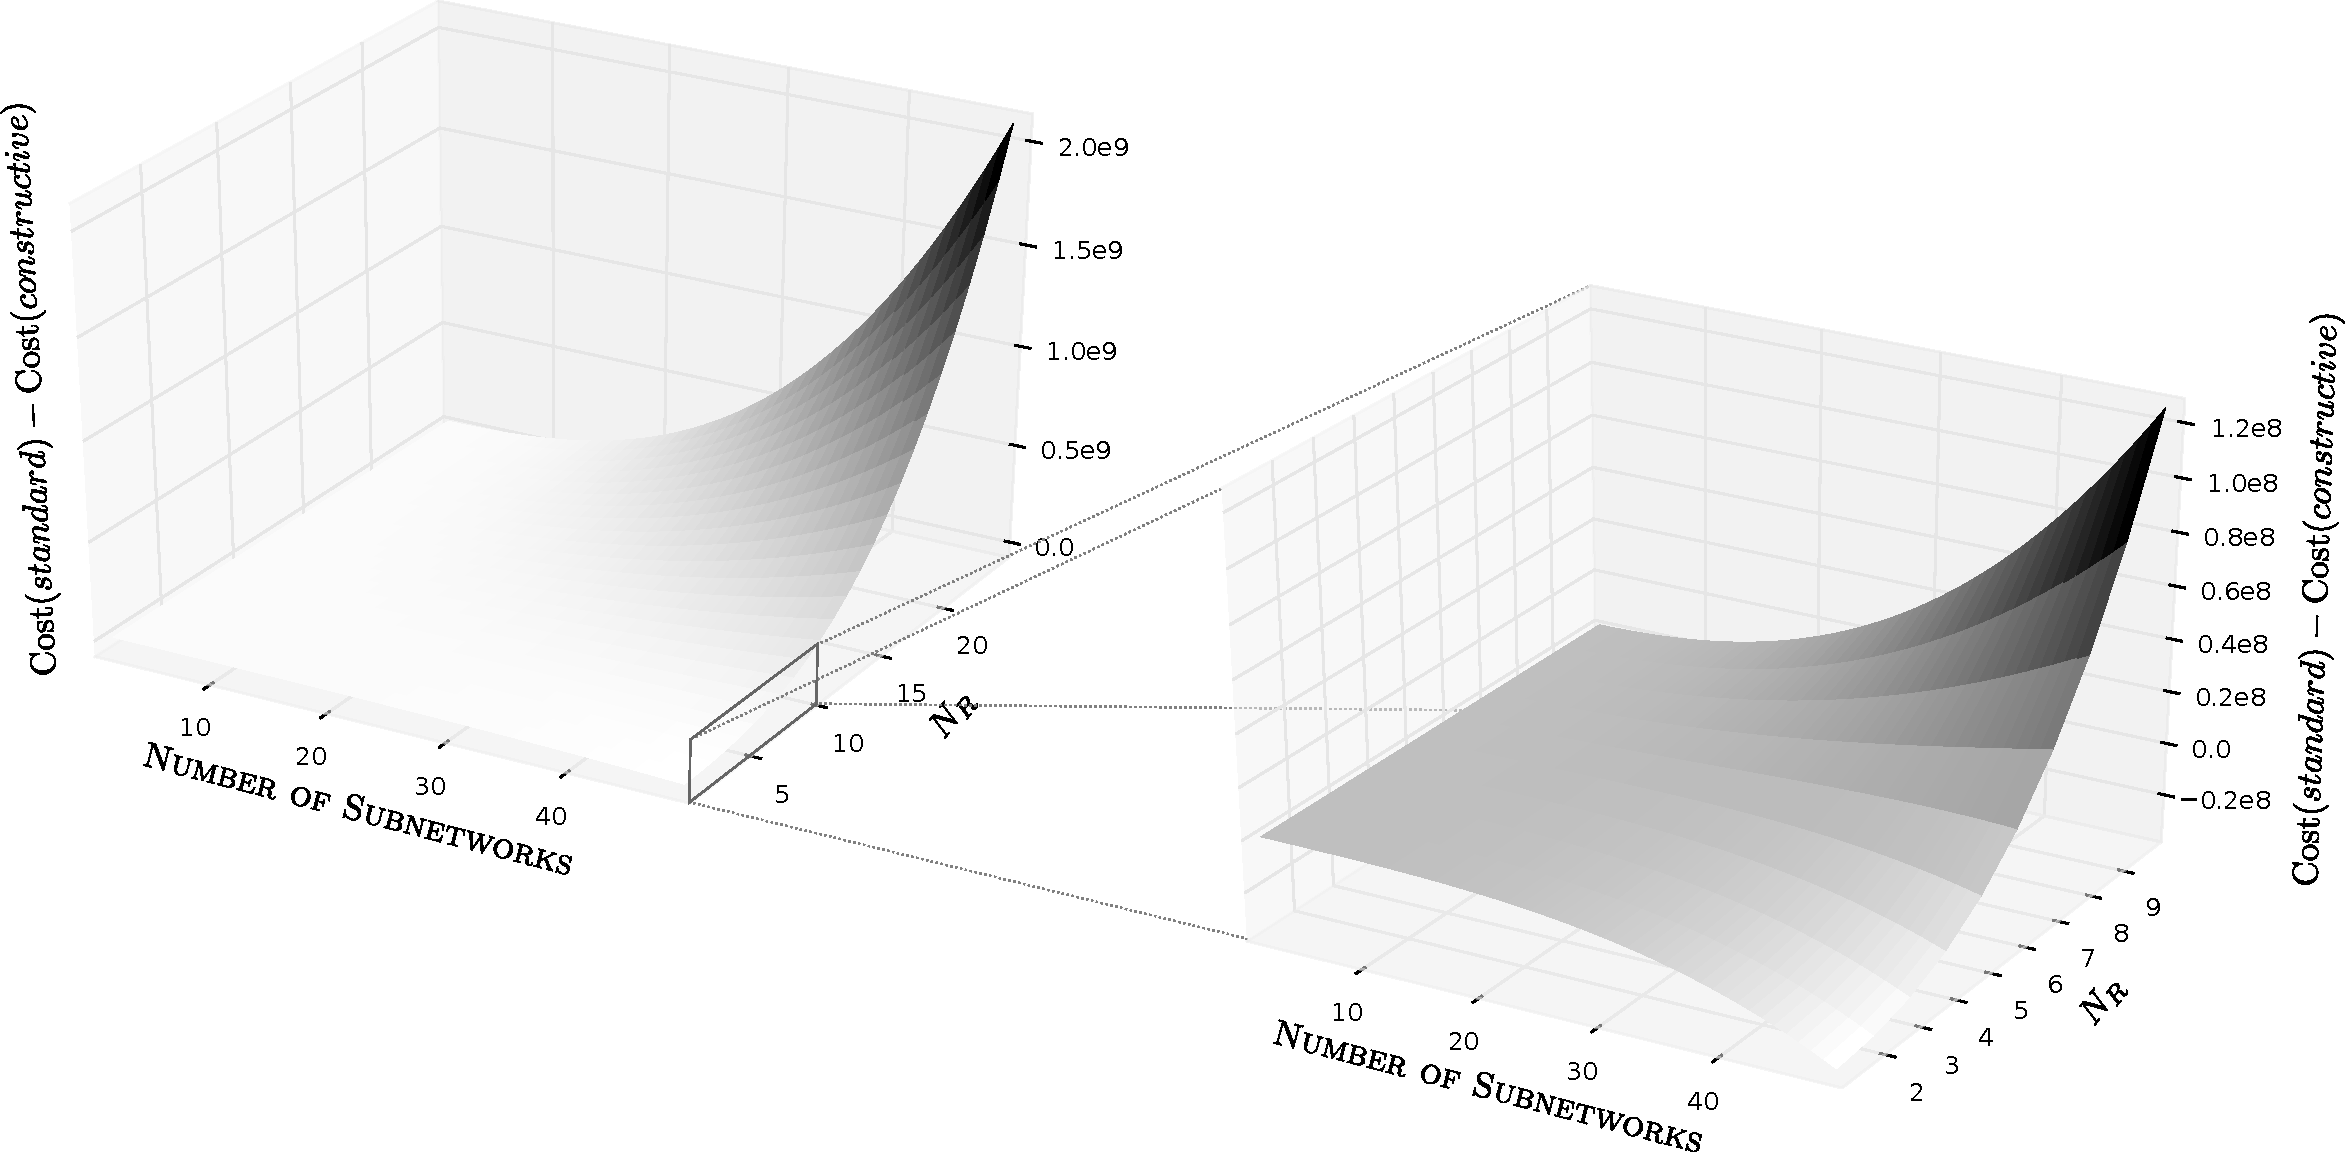
\includegraphics[width=1.0\columnwidth]{img/costo-v2}
\medskip
\caption[Approccio costruttivo: vantaggio computazionale]{Vantaggio computazionale nell'uso dell'approccio costruttivo. Assi orizzontali: numero di sotto-reti e dimensioni del reservoir ($N_R$). Asse verticale: differenza fra costo del modello standard e costo del modello costruttivo.\\
(\emph{sx}) $N_R \in [1,25]$. (\emph{dx}) Dettaglio della regione con minore vantaggio computazionale: $N_R \in [1,10]$.}
\label{fig:modelli:costo}
\end{figure}

La figura~\vref{fig:modelli:costo} dà un'intuizione di quale sia il vantaggio dal punto di vista computazionale derivato dall'adozione dell'approccio costruttivo. A parità di dimensioni del dataset (i.e.\ $\abs{\mathcal{G}} = 100$ ) ed al variare delle dimensioni dei reservoir e del numero delle sotto-reti, la figura mostra come varia la differenza fra il costo di una GraphESN standard equivalente (i.e.\ con reservoir di dimensione $N_R' = N_R\, \mathit{NSN}$) e di una GraphESN-FOF. I valori positivi corrispondono dunque ai casi in cui l'approccio costruttivo risulta più efficiente.\\
La figura evidenzia come con il crescere delle dimensioni dei reservoir ed all'aumentare del numero di sotto-reti, l'approccio costruttivo risulti in un vantaggio computazionale notevole. 
La possibilità di scomporre un problema in sotto-problemi si rispecchia infatti nella struttura complessiva della rete, che impiega, rispetto al caso delle GraphESN, più reservoir di dimensioni ridotte, il cui allenamento richiede un impiego minore di risorse di calcolo.
A destra nella figura è evidenziata tuttavia l'esistenza di particolari condizioni per le quali l'impiego di una strategia costruttiva risulta essere sconveniente. Tale situazione si verifica in particolare nel caso in cui si usino molte sotto-reti di dimensioni estremamente ridotte. La motivazione risiede nel fatto che, in un simile scenario, il costo computazionale complessivo risulta dominato dal processo iterativo di costruzione della rete piuttosto che dalla dimensione dei reservoir trattati. 
In merito a quanto detto è tuttavia opportuno osservare che, per la natura stessa del Reservoir Computing, l'impiego di reservoir con un numero davvero esiguo di unità è da considerarsi poco realistico.

Un'ulteriore osservazione risulta particolarmente importante per valutare i modelli proposti dal punto di vista computazionale. Benché il confronto con una singola GraphESN lasci emergere i vantaggi dei modelli proposti, è infatti opportuno sottolineare come la strategia costruttiva comporti particolari benefici anche in termini di selezione del modello. Per determinare la corretta dimensione della rete, infatti, i modelli non costruttivi si affidano ad un approccio \emph{trial and error} in cui ogni possibile variazione nella dimensione del reservoir viene allenata e valutata in maniera indipendente. Al contrario, l'approccio costruttivo permette di determinare la dimensione della rete in maniera automatica ed offre quindi l'opportunità di ridurre di molto il numero di esperimenti necessari a determinare quali siano gli iperparametri più adatti per la risoluzione di un task. \\
Intuitivamente possiamo dunque dire che il costo speso per la costruzione incrementale di una singola rete costruttiva, corrisponda all'allenamento ed il test di svariate reti diverse nel caso delle GraphESN. Per fare un esempio possiamo pensare che l'allenamento di una GraphESN-FOF, formata da $\mathit{NSN}$ sotto-reti di dimensione $N_R$, corrisponda, in termini computazionali, all'allenamento di $\mathit{NSN}$ diverse GraphESN, con reservoir di dimensioni crescenti: $N_R' \in \lbrace N_R, 2 N_R, \dots, \mathit{NSN}\, N_R \rbrace$.
Questo porta ad avere un costo complessivo per la selezione di una GraphESN pari a (si veda il paragrafo~\ref{app:costo:modelselection})
\begin{multline}
O(\mathit{NSN}^4\ N_R^3 + \mathit{NSN}^3\ N_R^2\ \mathit{MAXIT}\ \mathit{MAXV}\ \abs{\mathcal{G}} \\
+ \mathit{NSN}^3\ N_R^2\ \abs{\mathcal{G}} + \mathit{NSN}^2\ N_R\ \abs{\mathcal{G}}) 
\end{multline}
che scala con il prodotto fra $N_R^3$ e $\mathit{NSN}^4$ determinando una dipendenza estremamente svantaggiosa rispetto al caso dell'allenamento di una singola GraphESN-FOF, in cui i due fattori compaiono congiunti in una dipendenza al più quadratica.

Quanto detto evidenzia dunque come i modelli proposti si caratterizzino per efficienza dal punto di vista computazionale. La strategia costruttiva introdotta permette infatti di ridurre gli oneri del processo di apprendimento rispetto alle GraphESN, già di per sé contraddistinte dall'efficienza computazionale, rispondendo ad un'esigenza molto rilevante nell'ambito del trattamento dei domini strutturati. 
\`E infine opportuno sottolineare come l'utilizzo di uno schema di output-feedback permetta, nei modelli proposti, di influenzare il processo di encoding in maniera supervisionata senza che questo comporti la perdita, in termini computazionali, dei vantaggi derivati dall'uso di un reservoir non adattivo.



%%%%%%%%%%%%%%%%%%%%%%%%%%%%%%
\section{Software}\label{ch:modelli:software}
Un'implementazione software dei modelli descritti nel corso del capitolo è stata realizzata utilizzando il linguaggio \texttt{Python}\footnote{\url{http://python.org/}} (versione 2.6). 

Essendo un linguaggio dinamico, dalla sintassi semplice e fornito di un'ampia libreria standard, \texttt{Python} risulta particolarmente efficace per la prototipazione rapida. Questa caratteristica è stata considerata particolarmente desiderabile ai fini della realizzazione del lavoro svolto. Lo sviluppo dei modelli, così come quello del software, è infatti stato portato avanti in maniera incrementale, secondo un percorso guidato anche dall'esito di prove empiriche e sperimentali.

La scelta del linguaggio è risultata inoltre soddisfacente in termini di performance, nonostante il fatto che \texttt{Python} sia un linguaggio interpretato. L'utilizzo della libreria \texttt{scipy}\footnote{\url{http://www.scipy.org/}} per l'algebra lineare ha infatti permesso di raggiungere prestazioni comparabili con quelle ottenibili realizzando gli stessi modelli in \texttt{MATLAB}\footnote{\url{http://www.mathworks.com/products/matlab/}}, il cui utilizzo è ampiamente diffuso nell'ambito della realizzazione di modelli neurali.

Il software sviluppato sarà rilasciato con licenza open source.


%%%%%%%%%%%%%%%%%%%%%%%%%%%%%%%%%%%%%%%%%%%%%%%%%%%%%%%%%%%%%%%%%%%%%%%%%%%%%%%%
%%%%%%%%%%%%%%%%%%%%%%%%%%%%%%%%%%%%%%%%%%%%%%%%%%%%%%%%%%%%%%%%%%%%%%%%%%%%%%%%


\begin{comment}
Consideriamo una rete (FOF) formata da 'd' sotto-reti. Tutti i reservoir hanno
dimensione Nr, sia le sotto-reti che il readout-globale hanno output Ny, che
però è trascurabile.

--------------------------------------------------------------------------------

*** Convergenza del reservoir ***

La rete i-esima

    x_t(v) = f(Win u(v) + \sum_{w} W x_{t-1}(w) + Wfof z(g))

con:
    Win     :   (Nr, Nu)
    W       :   (Nr, Nr)
    Wfof    :   (Nr, Ny * (i-1))

Per un grafo g:
    Win u(v)                :   O(Nr Nu |V(g)|) - calcolato una sola volta
    Wfof z(g)               :   O(Nr Ny (i+1))  - calcolato una volta sola
    \sum_{w} W x_{t-1}(w)   :   O(Nr^2 |V(g)|)  - ad ogni iterazione

Chiamiamo 'j' il numero massimo di iterazioni e 'v' il numero massimo di 
vertici.
Il calcolo viene ripetuto per ogni grafo, quindi |G| volte.
La convergenza del reservoir i-esimo sull'intero grafo quindi costa:

    O(|G| (Nr Nu v + Nr Ny (i-1) + Nr^2 v j))
    ~ O(|G| Nr^2 v j)

gli output-feedback risultano trascurabili: quello che pesa è il processo 
iterativo del reservoir.
Il costo della convergenza di *tutte* le sotto-reti è dunque 'd' volte quello
di una singola sotto-rete:

    O(d |G| Nr^2 v j)


--------------------------------------------------------------------------------

*** Training (sotto-rete) ***

** Con Max-S
Per ogni iterazione (rete i-esima):
    Calcolo dell'output                         :   O(|G| (Nr + Ny (i-1)) Ny)
    Calcolo correlazione                        :   O(|G| Ny)
    Calcolo \sigma_o (E_po - \bar{E}_o) f'_p    :   O(|G| Ny)
    Calcolo gradiente                           :   O(|G| (Nr + Ny (i-1)) Ny) 

Mettendo tutto insieme, un'iterazione costa:

    O(|G| Ny (2 + (Nr + Ny (i-1))))
    ~ O(|G| Ny Nr + |G| i Ny^2)

Chiamiamo 'q' il numero massimo di iterazioni necessarie alla convergenza.
Il costo complessivo per l'applicazione dell'algoritmo a *tutte* le sotto-reti è

    O(q d |G| Ny Nr + q |G| Ny^2 d^2)
    ~ O(q d |G| Nr + q |G| d^2)         [Ny trascurabile]


** Con Ridge-Regression

    W.T = (A.T A + \lambda I)^-1 A.T B

con 

    A   :   (|G|, Nr + Ny (i-1)) = (|G|, Nf) 
    B   :   (|G|, Ny)

ho chiamato Nf = Nr + Ny (i-1) il numero di features in input al readout. E'
solo per comodità (n.b. Nf varia a sotto-rete a sotto-rete).

Costo:
    A.T A                           :   O(Nf^2 |G|)     [prodotto]
    (A.T A + \lambda I)^-1          :   O(Nf^3)         [inversione]
    A.T B                           :   O(Nf |G| Ny)    [prodotto]
    (A.T A + \lambda I)^-1 A.T B    :   O(Nf^2 Ny)      [prodotto]

Mettendo tutto insieme:

    O(Nf^3 + Nf^2 |G| + Nf^2 Ny + Nf |G| Ny)
    ~ O(Nf^3 + Nf^2 |G| + Nf^2 + Nf |G|)        [Ny trascurabile]
    ~ O(Nf^3 + Nf^2 |G|)

Cechiamo di calcolare il costo per tutta la rete, ovvero per 'd' sotto-reti.
Quanto vale Nf? Per l'unità i-esima: Nf = Nr + Ny (i-1)
Quindi:

Nf_1 = Nr
Nf_2 = Nr + Ny
Nf_3 = Nr + 2 Ny
Nf_4 = Nr + 3 Ny
...
Nf_d = Nr + (d-1) Ny

Quindi:

(Nf_1)^2 = Nr^2
(Nf_2)^2 = Nr^2 + Ny^2 + 2 Nr Ny
(Nf_3)^2 = Nr^2 + 4 Ny^2 + 4 Nr Ny
(Nf_3)^2 = Nr^2 + 9 Ny^2 + 6 Nr Ny
...
(Nf_d)^2 = Nr^2 + (d-1)^2 Ny^2 + 2 (d-1) Nr Ny

sommando: O(d Nr^2 + Ny^2 d^3  + Nr Ny d^2) 
            ~ O(d^3 + d^2 Nr + d Nr^2)      [Ny trascurabile]

Passiamo al cubo:

(Nf_1)^3 = Nr^3
(Nf_2)^3 = Nr^3 + Ny^3 + 3 Nr^2 Ny + 3 Nr Ny^2
(Nf_3)^3 = Nr^3 + 8 Ny^3 + 6 Nr^2 Ny + 12 Nr Ny^2
(Nf_3)^3 = Nr^3 + 27 Ny^3 + 9 Nr^2 Ny + 27 Nr Ny^2
...
(Nf_d)^3 = Nr^3 + (d-1)^3 Ny^3 + 3 (d-1) Nr^2 Ny + 3 (d-1)^2 Nr Ny^2

sommando: O(d Nr^3 + Ny^3 d^4 + Nr^2 Ny d^2 + Nr Ny^2 d^3)
            ~ O(d^4 + Nr d^3 + Nr^2 d^2 + Nr^3 d)       [Ny trascurabile]

Mettendo tutto insieme, il costo del training di tutte le sotto-reti tramite
ridge-regression è

    O(d^4 + Nr d^3 + Nr^2 d^2 + Nr^3 d + d^3 |G| + d^2 Nr |G| + d Nr^2 |G|)



--------------------------------------------------------------------------------

*** Training (readout-globale) ***

** Con Ridge-Regression

Come il caso precedente, ma senza alcun reservoir (i.e.\ solo gli output-feedback
in input)

    O(Nf^3 + Nf^2 |G|) con Nf = Ny (i-1) per la sotto-rete i-esima

Quindi:

    O(Ny^3 d^4 + Ny^2 d^3 |G|)
    ~ O(d^4 + d^3 |G|)          [Ny trascurabile]


** Con LMS

Per un singolo allenamento, dopo aver aggiunto la sotto-rete i-esima:

    O(|G| Nf Ny) = O(r |G| (i-1) Ny^2)

con 'r' numero massimo di iterazioni per la convergenza.

Complessivamente il costo è:

    O(r |G| d^2 Ny^2)
    ~ O(r |G| d^2)    [Ny trascurabile]


--------------------------------------------------------------------------------

*** Calcolo dell'output (sotto-rete) ***

Tutti i valori in input sono precalcolati (reservoir + output-feedback).
Il costo è quello della moltiplicazione:

    Wout [X(x(g)), z_1(g), ... , z_{i-1}(g)] = Wout in

con:
    Wout    :   (Ny, Nr + Ny (i-1))
    in      :   Nr + Ny (i-1)

Quindi per una rete ed un input:

    O(Ny (Nr + Ny (i-1)))
    = O(Ny Nr + Ny^2 (i-1))

Il costo del calcolo dell'output di *tutte* le 'd' sotto-reti è dunque:

    O(|G| ((Ny Nr) + (Ny Nr + Ny^2) + (Ny Nr + 2 Ny^2) + ... + (Ny Nr + (d-1) Ny^2))))
    = O(|G| (d Ny Nr + Ny^2 d^2))
    ~ O(d Nr |G| + d^2 |G|)         [Ny trascurabile]


--------------------------------------------------------------------------------

*** Calcolo dell'output (readout globale) ***

Differisce dal caso precedente solo perché ha in input unicamente gli 
output-feedback, quindi nessun reservoir.

    O(Ny^2 d^2 |G|)
    ~ O(d^2 |G|)


********************************************************************************
********************************************************************************

*** Confronto: Costruttivo VS Standard ***

** GraphESN Costruttiva

reservoir:          O(d |G| Nr^2 v j)
sub learning:       O(d^4 + Nr d^3 + Nr^2 d^2 + Nr^3 d + d^3 |G| + d^2 Nr |G| + d Nr^2 |G|) 
gloabl learning:    O(d^4 + d^3 |G|) 
sub output:         O(d Nr |G| + d^2 |G|) 
global output:      O(d^2 |G|) 

** GraphESN Stadard

reservoir:          O(d |G| Nr^2 v j) (???) O(|G| (d Nr)^2 )
learning:           O(Nr^3 + Nr^2 |G|)
output:             O(|G| Nr)

\end{comment}



 \chapter{Risultati Sperimentali}\label{ch:esperimenti}
Il capitolo illustra e discute i risultati sperimentali ottenuti applicando i modelli proposti su task relativi a dataset reali.

Il paragrafo~\ref{sec:esperiment:dataset} descrive i dataset utilizzati ed i corrispondenti task affrontati.

Il paragrafo~\ref{sec:esperiment:esperimenti} descrive i setting sperimentali e raccoglie i risultati ottenuti.

Il paragrafo~\ref{sec:esperiment:considerazioni} espone un'analisi critica dei risultati sperimentali.


%%%%%%%%%%%%%%%%%%%%%%%%%%%%%%%%%%%%%%%%%%%%%%%%%%%%%%%%%%%%%%%%%%%%
\section{Dataset}\label{sec:esperiment:dataset}
Le potenzialità dei modelli proposti sono state sperimentate su problemi reali appartenenti all'ambito della Chimica. 

Pur senza addentrarsi nei dettagli è interessante sottolineare come il legame fra il Machine Learning e la Chimica vada recentemente rafforzandosi, in particolar modo in relazione all'apprendimento di dati su domini strutturati. L'enorme varietà di molecole naturalmente rappresentabili come grafi, i costi sperimentali elevati, l'esistenza di conoscenze non sempre codificabili o prone a numerose eccezioni, fanno infatti della Chimica il banco di prova ideale per dei modelli in grado di gestire domini strutturati.

\`E dunque alla sfera della Chemioinformatica che vanno ascritti i task affrontati ed i dataset che verranno descritti nel seguito del paragrafo.

Prima di procedere, è importante sottolineare che nessuna specifica conoscenza pregressa è stata necessaria per preprocessare i dati, modificarne la struttura o estrapolarne informazioni numeriche. In altri termini, le informazioni utilizzate per allenare i modelli sono esattamente quelle riportate nei dataset: diversamente da quanto accade ricorrendo ad altri approcci, nessuna particolare assunzione riguardante il dominio trattato è stata fatta (e.g.\ la scelta di una metrica nell'uso di un kernel) né è stata praticata alcuna forma di feature-selection manuale (e.g.\ la selezione di indici topologici).

\subsubsection*{Predictive Toxicology Challenge}\label{sec:esperimenti:dataset:ptc}
Il \emph{Predictive Toxicology Challenge} (PTC) \cite{Helma:ThePTC} ha fornito i dati per quattro task distinti. Il dataset consta di $417$ molecole in formato \emph{Structure Data Format} (SDF) di cui è riporta la carcinogenicità riferita a diversi tipi di roditori: topi maschi (MM), topi femmine (FM), ratti maschi (MR), ratti femmine (FR). 

Ogni molecola è stata rappresentata come un grafo indiretto, con i vertici corrispondenti agli atomi e gli archi ai legami atomici. Il grado massimo riscontrato sull'intero dataset è $k = 4$. Il numero di vertici nei grafi in input risulta mediamente $25.7$, variando da un minimo di $2$ ad un massimo di $109$.

L'etichetta numerica associata ad ogni vertice è stata ottenuta codificando il simbolo atomico corrispondente tramite un encoding binario $1$-of-$m$ e concatenando due valori aggiuntivi presenti nel dataset, CHG e RAD, rispettivamente corrispondenti alla carica atomica ed il radical dell'atomo. La dimensione totale delle etichette di input è dunque $24$. 
La figura~\ref{fig:molecole} mostra l'esempio due molecole appartenenti al dataset PTC, rappresentate come grafi indiretti, e schematizza il processo di encoding del simbolo atomico.
\begin{figure}[tbp]
\centering
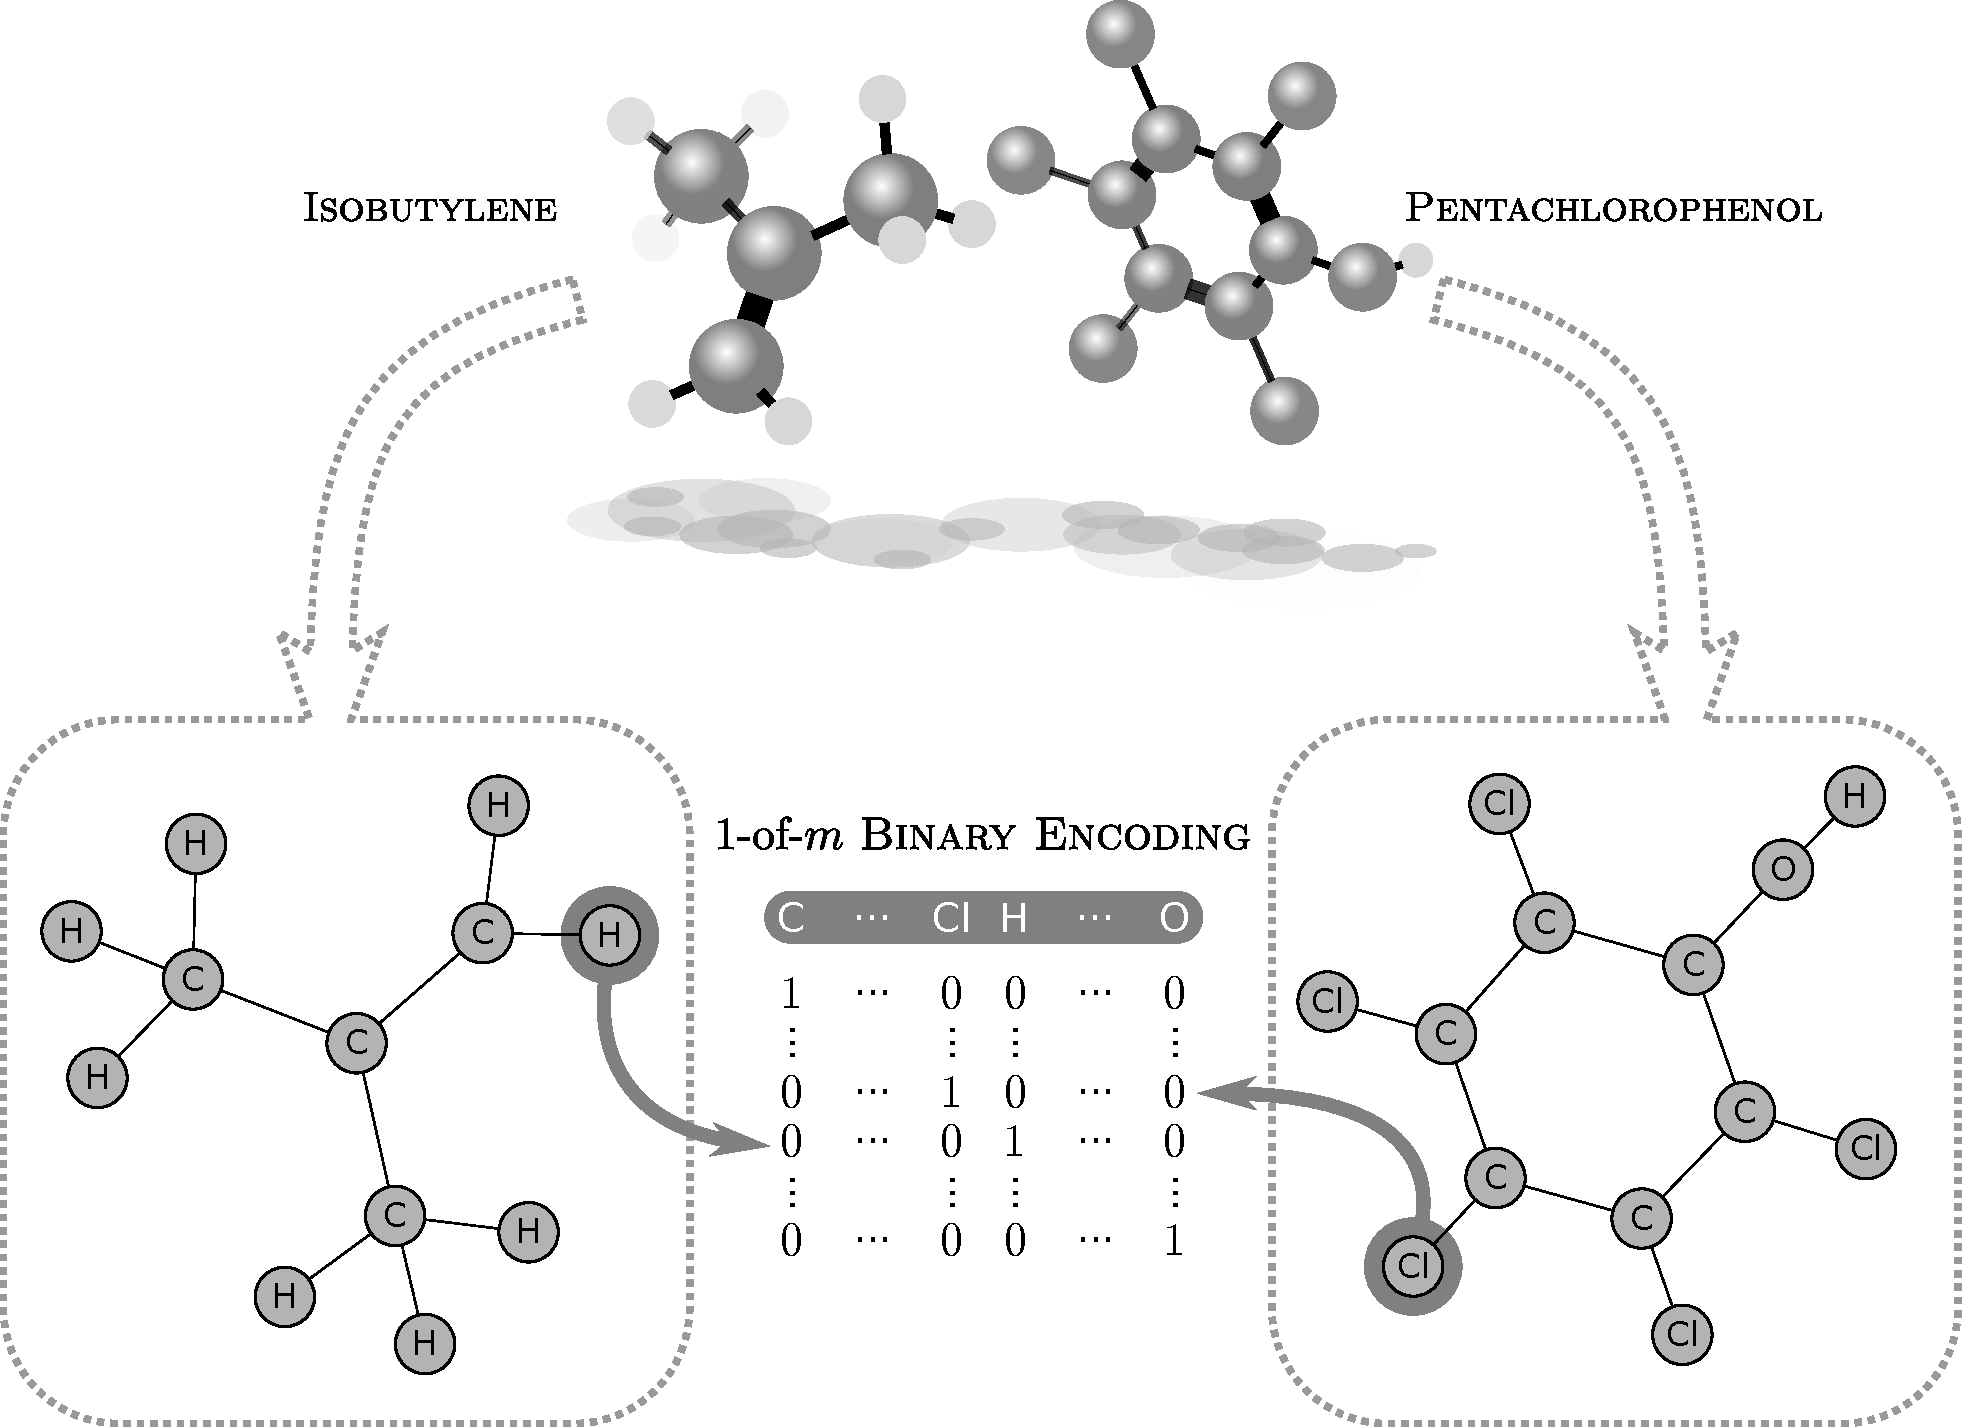
\includegraphics[width=0.9\columnwidth]{img/molecole-v2}
\medskip
\caption[Rappresentazione dell'input]{Rappresentazione dell'input in forma di grafo ed encoding del simbolo atomico.}
\label{fig:molecole}
\end{figure}

Quattro task structure-to-element di classificazione binaria sono stati definiti per PTC, uno per ogni tipo di roditore \cite{Frohlich:OptimalAssignment}, assegnando target $+1$ alle molecole attive e target $-1$ a quelle inattive.

\subsubsection*{Mutagenesis}\label{sec:esperimenti:dataset:mutag}
La seconda serie di task affrontati si riferisce al dataset \emph{Mutagenesis} \cite{Srinivasan:Mutagenesis} (Mutag), contenente 230 molecole nitroaromatiche in formato Progol\footnote{\url{http://www.doc.ic.ac.uk/~shm/progol.html}}, di cui è indicata la mutagenicità.
Ogni composto nel dataset è descritto dalla sua struttura atomo-legame (AB), da due valori corrispondenti a misurazioni di proprietà chimiche della molecola (C) e due attributi strutturali precalcolati (PS). Riprendendo quanto fatto in \cite{Gallicchio:GraphESN}, sono state dunque considerate le tre possibili descrizioni: AB, AB+C, AB+C+PS.

Ogni molecola del dataset è stata rappresentata come un grafo indiretto, con vertici ed archi corrispondenti ad atomi e legami rispettivamente, entrambi riportati nella descrizione AB dei singoli composti. Il grado massimo riscontrato sul dataset risulta essere $k = 4$. Il numero di vertici per input varia tra un minimo di $13$ ad un massimo di $40$, con una media di $25.6$ vertici per ogni molecola.

L'etichetta numerica associata ad ogni vertice dell'input è stata ricavata codificando il simbolo atomico corrispondente attraverso un encoding binario $1$-of-$m$ e poi concatenando la carica parziale dell'atomo, il tipo atomico normalizzato in $[-1,1]$ più gli altri valori globali contenuti nella descrizione C e PS, in accordo alla rappresentazione via via adottata. La dimensione delle etichette di input è dunque di 11, 13 e 15 per le descrizioni AB, AB+C e AB+C+PS rispettivamente.

Il task sul dataset è stato definito come una classificazione binaria, con il target a $+1$ per i grafi corrispondenti a composti mutageni e $-1$ altrimenti.



\subsubsection*{Bursi}\label{sec:esperimenti:dataset:bursi}
Il dataset \emph{Bursi} \cite{Kazius:Bursi,Ferrari:AnOpenSource} contiene 4204 molecole in formato SDF, di cui è riportata la mutagenicità. Ne risulta un task structure-to-element di classificazione binaria.
Il dataset risulta all'origine suddiviso partizionato in un training-set, contenente 3367 molecole, ed un test-set con 837 composti.

Anche in questo caso le molecole sono state rappresentate come grafi indiretti, con vertici ed archi corrispondenti ad atomi e legami rispettivamente. Nell'input il numero di vertici varia tra un minimo di $4$ ed un massimo di $417$, con una media di $30.3$ vertici per molecola.

L'etichetta numerica associata ai vertici è realizzata attraverso l'encoding binario $1$-of-$m$ del simbolo atomico. Le etichette hanno dunque dimensione $14$. Il grado massimo riscontato sul dataset è $k = 4$.

Il target per il task di classificazione binaria è stato realizzato assegnando valore $+1$ alle molecole attive e $-1$ alle molecole non attive.


\subsubsection*{Angiotensin Converting Enzyme}\label{sec:esperimenti:dataset:ace}
Il dataset \emph{Angiotensin Converting Enzyme} (ACE) \cite{Sutherland:AComparisonOfMethods} contiene 114 ACE-inibitori in formato SDF a cui è associato un valore reale che ne indica l'attività (i.e.\ $\text{plC}_{50}$) in un intervallo che varia tra $2.1$ a $9.9$. Il dataset definisce dunque un task structure-to-element di regressione di tipo \emph{Quantitative Structure–Activity Relationship} (QSAR).

Come nei casi precedenti, le molecole sono state rappresentate come grafi indiretti, con i vertici corrispondenti agli atomi e gli archi corrispondenti ai legami. Il grado massimo riscontrato sul dataset è $k=4$, le dimensioni dei grafi variano tra $18$ e $79$, con una media di $42.5$ vertici per input.

I valori dell'etichetta associata ad ogni vertice dell'input sono ricavati concatenando l'encoding binario del simbolo atomico al valore della carica atomica, CHG, presente nel dataset. Le etichette di input hanno dunque dimensione $8$.



%%%%%%%%%%%%%%%%%%%%%%%%%%%%%%%%%%%%%%%%%%%%%%%%%%%%%%%%%%%%%%%%%%%%
\section{Esperimenti}\label{sec:esperiment:esperimenti}
Sui dataset descritti in precedenza sono stati svolti esperimenti che permettessero di confrontare i tre modelli proposti (si veda il paragrafo~\ref{sec:modelli:modelli}) con le GraphESN (paragrafo~\ref{sec:intro:struct:gesn}). 

\`E bene precisare che, data la flessibilità dell'approccio introdotto, sono molte le diverse strategie applicabili per realizzare un singolo modello fra quelli descritti. Variazioni sono possibili nell'inizializzazione dei pesi, nella scelta delle candidate, nella tipologia di allenamento delle sotto-reti o nel task loro assegnato. Tutte le reti a cui fanno riferimento i risultati riportati nel seguito condividono dunque un setting sperimentale comune, che individua solo un piccolo frammento delle possibili varianti implementative. Prima di presentare i risultati sperimentali è quindi necessario descrivere il setting sperimentale adottato.

Come appartenenti all'ambito del Reservoir Computing, le reti considerate presentano una serie di connessioni i cui pesi non vengono modificati durante il learning: le connessioni input-reservoir e reservoir-reservoir, a cui si aggiungono, nei modelli proposti, anche le connessioni per gli output-feedback. \\
Nei modelli sperimentati i pesi sulle connessioni di input, contenuti nella matrice $\matr{W}_\textup{in}^{(i)}$ per la sotto-rete $i$-esima, hanno valori random con distribuzione uniforme nell'intervallo $[-\lambda_\textup{in}, \lambda_\textup{in}]$, con $\lambda_\textup{in}$ parte degli iperparametri del modello. I pesi sulle connessioni del reservoir, matrice $\hat{\matr{W}}^{(i)}$, sono invece stati inizializzati secondo una distribuzione uniforme in $[-1,1]$ e poi ridimensionati per ottenere il coefficiente di contrazione $\sigma$ desiderato (si veda l'equazione (\ref{eq:intro:gesn:sigma}) a pagina~\pageref{eq:intro:gesn:sigma}). In tutti gli esperimenti svolti si è ricorso a reservoir completamente connessi, sfruttando la possibilità di impiegare sotto-reti di dimensioni contenute, che non richiedessero eccessivi oneri computazionali.\\
Alle connessioni di output-feedback, in $\matr{W}_\textup{fof}^{(ij)}$ per ogni coppia di sotto-reti $(i,j)$, sono stati assegnati pesi fissi con valore dato dall'iperparametro $\lambda_\textup{fof}$.

Poiché tutti i dataset trattati riguardano trasduzioni structure-to-element, i modelli sperimentati ricorrono all'uso di una \textit{state mapping function}, $\mathcal{X}$. In tutti i casi è stata utilizzata una funzione \emph{mean state mapping} (si veda l'equazione~(\ref{eq:meanstate}) a pagina \pageref{eq:meanstate}).

I modelli costruttivi proposti sono caratterizzati da due distinte fasi di apprendimento per ogni iterazione: una riguardante le singole sotto-reti e l'altra relativa al readout globale (si veda l'algoritmo~\vref{alg:modelli:constr}).\\
Nel corso degli esperimenti svolti le sotto-reti sono state allenate attraverso l'algoritmo di Ridge Regression (si veda il paragrafo~\ref{intro:alg}) per emulare l'errore residuo commesso dalla rete. Il parametro di regolarizzazione $\lambda_\textup{r}$ utilizzato, uguale per ogni sotto-rete, rappresenta uno degli iperparametri dei modelli. La possibilità di usare un algoritmo di apprendimento che non dipendesse dal valore iniziale dei pesi e che non non rischiasse di convergere a minimi o massimi locali ha inoltre fatto propendere per tralasciare l'impiego di un pool di sotto-reti candidate.\\
Il readout globale è invece stato allenato tramite Least Mean Squares (LMS) con l'iperparametro $\lambda_\textup{wd}$ a regolare il \textit{weight decay} (si veda il paragrafo~\ref{intro:alg}).

Per tutte le unità, sia nei reservoir che nei readout, la funzione di attivazione utilizzata è la \emph{tangente iperbolica} ($\tanh$). L'errore residuo, utilizzato per l'allenamento delle sotto-reti, è dunque quello ottenuto dalla differenza fra l'attivazione delle unità di output ed il valore del target
\begin{equation}
\begin{split}
\vect{e}^{(i)}(\graph{g}) 
	&= \vect{y}^{(i)}(\graph{g}) - \vect{y}_\textup{target}(\graph{g}) \\
	&= \tanh( \matr{W}_\textup{out} \, [\vect{z}^{(1)}(\graph{g}), \dots, \vect{z}^{(i)}(\graph{g})] ) - 
		\vect{y}_\textup{target}(\graph{g})
\end{split}
\end{equation}
Ne risulta un errore distribuito nell'intervallo $(-2, 2)$. Due fattori influenzano la scelta di adottare tale criterio nel determinare l'errore, e dunque il target delle sotto-reti: da una parte la pratica ha lasciato emergere una minore efficacia dell'uso di errori discreti (e.g.\ $\vect{e}^{(i)}(\graph{g}) \in \lbrace -1, 1 \rbrace$ oppure $\vect{e}^{(i)}(\graph{g}) \in \lbrace -1, 0, 1 \rbrace$), dall'altra la necessità di usare un'arcotangente iperbolica, $\tanh^{-1}$, per per poter applicare la Ridge Regression nelle sotto-reti ha reso indispensabile la presenza di un limite, sia superiore che inferiore, sui valori di errore. Per essere efficacemente usato come target per le sotto-reti, dunque, il segnale di errore è stato ad ogni iterazione dimezzato e portato nell'intervallo $(-1,1)$.

Nel corso degli esperimenti svolti le reti sono state fatte crescere finché non si sia verificata una delle seguenti condizioni: l'errore sul training-set (i.e.\ misclassification-rate o errore quadratico medio), $\vect{e}^{(i)}(\mathcal{G}_\textup{tr})$, sia risultato inferiore ad una soglia prefissata, $\delta_\textup{err}$, specifica per ogni task, oppure la variazione dell'errore di training sia risultata, in due iterazioni successive, inferiore in valore assoluto ad un parametro $\delta_\textup{var}$. \`E inoltre stato fissato un numero massimo di sotto-reti, $\delta_\textup{size}$. In formula, il processo di costruzione della rete viene dunque interrotto quando si verifica la seguente condizione
\[
\vect{e}^{(i)}(\mathcal{G}_\textup{tr}) < \delta_\textup{err}
\ \vee\
\left\lvert \dfrac{\vect{e}^{(i)}(\mathcal{G}_\textup{tr}) - \vect{e}^{(i-1)}(\mathcal{G}_\textup{tr})}{\vect{e}^{(i)}(\mathcal{G}_\textup{tr})} \right\rvert < \delta_\textup{var}
\ \vee\
i = \delta_\textup{size}
\]

Per confrontare i modelli introdotti con le GraphESN, son stati svolti su queste ultime esperimenti che prevedessero l'impiego di iperparametri simili. L'allenamento delle GraphESN è stato realizzato tramite Ridge Regression e, per ovviare al fatto che in questo caso il numero di unità totali dovesse essere fissato a priori, sono state prese in considerazione diverse GraphESN facendo variare la dimensione del reservoir. 



%%%%%%%%%%%%%%%%%%%%%%%%%%%%%%%%%%%%%%
\subsection{Predictive Toxicology Challenge}
La valutazione dei modelli sui quattro task PTC è stata fatta attraverso una \emph{doppia k-fold cross-validation} (si veda il paragrafo~\ref{intro:validazione}) con un ciclo esterno di 5 fold ed un ciclo interno di 5 fold. La suddivisione del dataset è stata realizzata attraverso \emph{stratificazione} (si veda il paragrafo~\ref{intro:validazione}), in modo da garantire la stessa distribuzione di esempi positivi e negativi in ogni sotto-insieme.
Ogni iperparametrizzazione è stata testata su 5 istanziazioni del modello, in modo da variare i valori dei pesi random assegnati alle connessioni. 

Per ognuno dei modelli proposti sono state considerate due distinte configurazioni per la dimensione del reservoir delle sotto-reti: $N_R \in \lbrace 50, 30 \rbrace$. Il task structure-to-element di classificazione binaria prevede una dimensione delle etichette di input $N_U = 24$ e un singolo valore di uscita $N_Y = N_Z = 1$.

Per la convergenza del reservoir è stata adottata una soglia $\epsilon = 10^{-5}$. Il coefficiente di contrazione utilizzato è $\sigma = 1$.

Per interrompere la costruzione delle reti si è fissato $\delta_\textup{var} = 0.01$ e $\delta_\textup{tr}$, riferito al miscalssification-rate (i.e.\ rapporto fra input non classificati correttamente ed input totali), uguale a $0.29$, $0.33$, $0.37$,  $0.29$ per i task FR, FM, MR, MM rispettivamente. Il numero massimo di sotto-reti è stato fissato a $\delta_\textup{size} = 15$ nei casi in cui $N_R = 50$ e $\delta_\textup{size} = 20$ con $N_R = 30$.

Nell'allenamento del readout globale tramite LMS è stato utilizzato un learning-rate $\eta = 10^{-3}$.

La model selection ha coinvolto gli iperparametri $\lambda_\textup{in}$, $\lambda_\textup{fof}$, $\lambda_\textup{r}$, $\lambda_\textup{wd}$, fatti variare secondo i valori riportati nella tabella~\ref{tab:esperimenti:grigliaPTC}.
\begin{table}[tbp]
\small
\caption[Model selection: iperparametri per PTC]{Iperparametri usati per la model selection sui 4 task PTC.}
\label{tab:esperimenti:grigliaPTC}
\centering
\begin{tabular}{*{4}{c}}
\toprule
$\lambda_\textup{in}$ & $\lambda_\textup{fof}$ & $\lambda_\textup{r}$ & $\lambda_\textup{wd}$ \\
\midrule
$\lbrace 1.0, 0.1 \rbrace$ & $\lbrace 1.0, 2.0 \rbrace$ & $\lbrace 0.01, 0.1, 0.2 \rbrace$ & $\lbrace 0.0, 0.01 \rbrace$ \\
\bottomrule
\end{tabular}
\end{table}
Per realizzare la selezione del modello e la validazione dei risultati sono dunque state allenate $24200$ differenti istanziazioni di modelli costruttivi.

Sulle GraphESN la selezione del modello è stata eseguita facendo variare i valori di $N_R$, $\lambda_\textup{in}$, $\lambda_\textup{r}$ come indicato nella tabella~\ref{tab:esperimenti:grigliaPTCstandard}.
\begin{table}[tbp]
\small
\caption[Model selection: iperparametri per GraphESN su PTC]{Iperparametri per la model selection di GraphESN sui 4 task PTC.}
\label{tab:esperimenti:grigliaPTCstandard}
\centering
\begin{tabular}{*{3}{c}}
\toprule
$N_R$ & $\lambda_\textup{in}$ & $\lambda_\textup{r}$ \\
\midrule
$\lbrace 500, 200, 100, 50 \rbrace$ & $\lbrace 1.0, 0.1 \rbrace$ & $\lbrace 0.01, 0.1, 0.2 \rbrace$ \\
\bottomrule
\end{tabular}
\end{table}

La tabella~\ref{tab:esperimenti:ptc} descrive i risultati sperimentali ottenuti dai modelli sui quattro task PTC. I valori riportati rappresentano l'accuratezza percentuale di test (i.e.\ percentuale di grafi nel test-set classificata correttamente) mediata sulle $5$ fold e la deviazione standard media. Le tabelle~\ref{app:esp:PTC-FR-CF}-\ref{app:esp:PTC-MM-FOF} (si veda l'appendice~\vref{app:esperimenti}) riportano i risultati in dettaglio, fold per fold, dei vari modelli.
\begin{table}[tbp]
\small
\caption[Accuratezza media su PTC]{Accuratezza media dei modelli e deviazione standard, in percentuale, sui 4 task PTC.}
\label{tab:esperimenti:ptc}
\centering	
\begin{tabular}{l*{5}{c}}
\toprule
Model 		& $N_R$	& FR				 & FM				  & MR				   & MM	\\
\midrule
GraphESN 	& 	    & $67.7$ ($\pm 0.1$) & $60.7$ ($\pm 0.4$) & $56.7$ ($\pm 0.9$) & $67.1$ ($\pm 0.1$) \\
GraphESN-CF & $50$  & $67.3$ ($\pm 0.6$) & $62.8$ ($\pm 0.8$) & $57.9$ ($\pm 0.7$) & $65.0$ ($\pm 0.5$) \\
GraphESN-CF & $30$  & $67.2$ ($\pm 0.7$) & $63.2$ ($\pm 0.8$) & $58.1$ ($\pm 0.4$) & $65.8$ ($\pm 0.7$) \\
GraphESN-FW & $50$  & $67.1$ ($\pm 1.0$) & $63.6$ ($\pm 0.7$) & $58.4$ ($\pm 0.7$) & $65.4$ ($\pm 1.6$) \\
GraphESN-FW & $30$  & $67.2$ ($\pm 1.1$) & $63.3$ ($\pm 1.0$) & $57.4$ ($\pm 1.5$) & $64.6$ ($\pm 1.5$) \\
GraphESN-FOF & $50$ & $68.3$ ($\pm 1.1$) & $62.5$ ($\pm 1.2$) & $57.2$ ($\pm 1.3$) & $66.6$ ($\pm 1.7$) \\
GraphESN-FOF & $30$ & $67.9$ ($\pm 1.5$) & $62.8$ ($\pm 1.6$) & $57.4$ ($\pm 1.7$) & $65.4$ ($\pm 1.6$) \\
\bottomrule
\end{tabular}
\end{table}
Dai dati si riscontra come i modelli introdotti risultino in grado, in tre dei quattro casi, di migliorare la performance predittiva ottenuta tramite un approccio non costruttivo. In due dei quattro casi esaminati (i.e.\ FM, FR) il miglioramento offerto dai modelli costruttivi risulta sistematico e consistente se si considera che il dataset è particolarmente affetto da rumore.

La tabella~\ref{tab:dimensioni:mutag} riporta i dati relativi alle dimensioni raggiunte delle reti nell'affrontare i quattro task del dataset.
\begin{table}
\small
\caption[Dimensioni delle reti su PTC]{Numero di sotto-reti dei modelli sui quattro task PTC. Numero massimo, numero minimo, media e moda.}
\label{tab:dimensioni:ptc} 
\centering	
\begin{tabular}{l*{4}{c}}
\toprule
Model 		 & Max & Min & Avg & Mode \\
\midrule
GraphESN-CF  & $15$ & $2$ & $3.9$ & $3$ \\
GraphESN-FW  & $20$ & $2$ & $5.2$ & $3$ \\
GraphESN-FOF & $20$ & $2$ & $4.6$ & $3$ \\
\bottomrule
\end{tabular}
\end{table}
Si nota come in alcuni casi le reti crescano abbastanza da raggiungere la dimensione massima imposta $\delta_\textup{size}$, suggerendo l'eventuale adozione di una soglia meno vincolante.

La figura~\vref{fig:esperimenti:plot-ptc} mostra alcuni esempi di curve di apprendimento riferite all'applicazione su PTC del più generale dei modelli proposti (i.e.\ GraphESN-FOF). L'errore riportato è il misclassification-rate, motivo per cui le curve di test, calcolate su pochi dati, risultano avere un andamento caratterizzato da forti pendenze. Come mostrato in figura, il processo incrementale di costruzione della rete risulta efficace nell'aumentare la capacità di generalizzazione della rete, ma non evita completamente il verificarsi di situazioni di overfitting (grafico al centro).
\begin{figure}[p]
\centering
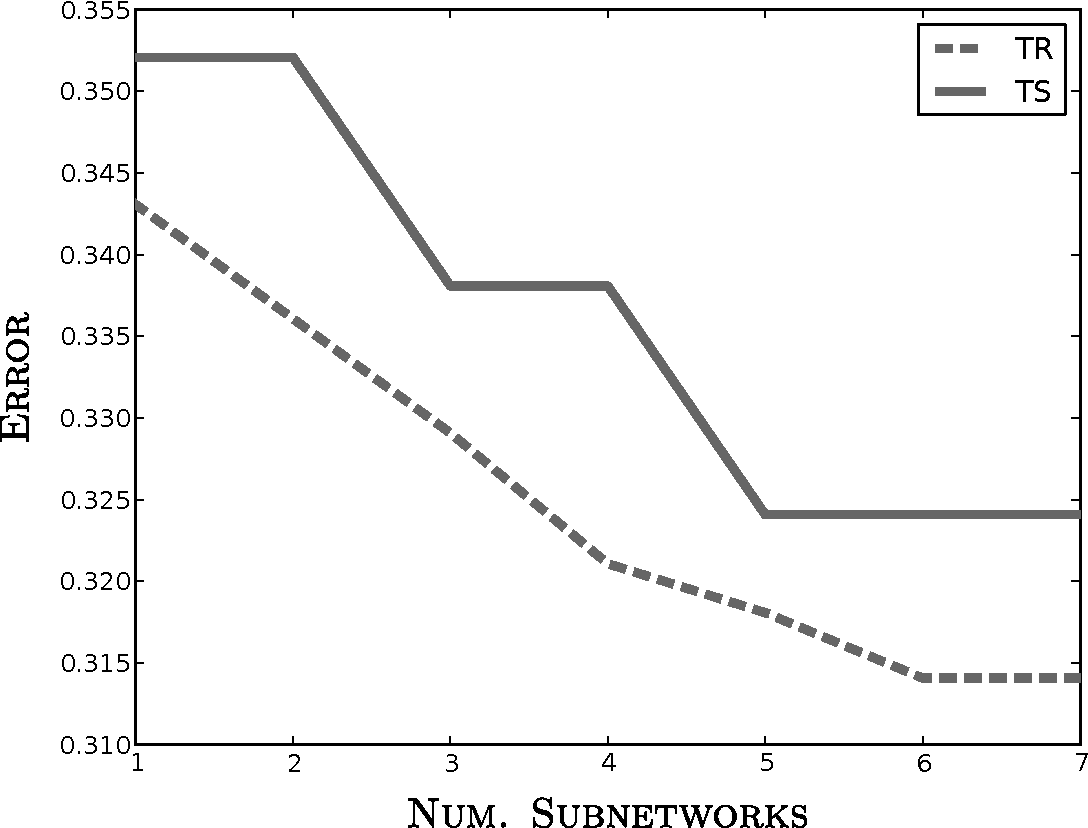
\includegraphics[width=0.5\columnwidth]{img/plot/ptc1}\\
\vspace*{0.8cm}
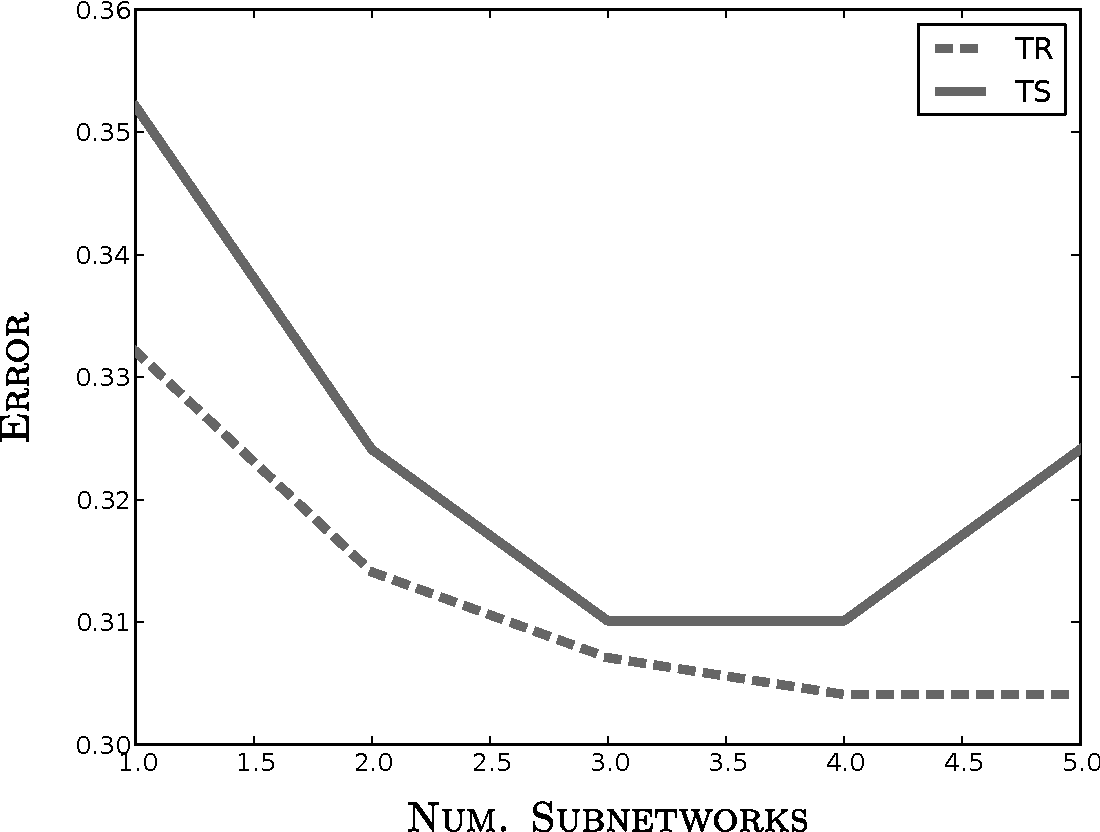
\includegraphics[width=0.5\columnwidth]{img/plot/ptc2}\\
\vspace*{0.8cm}
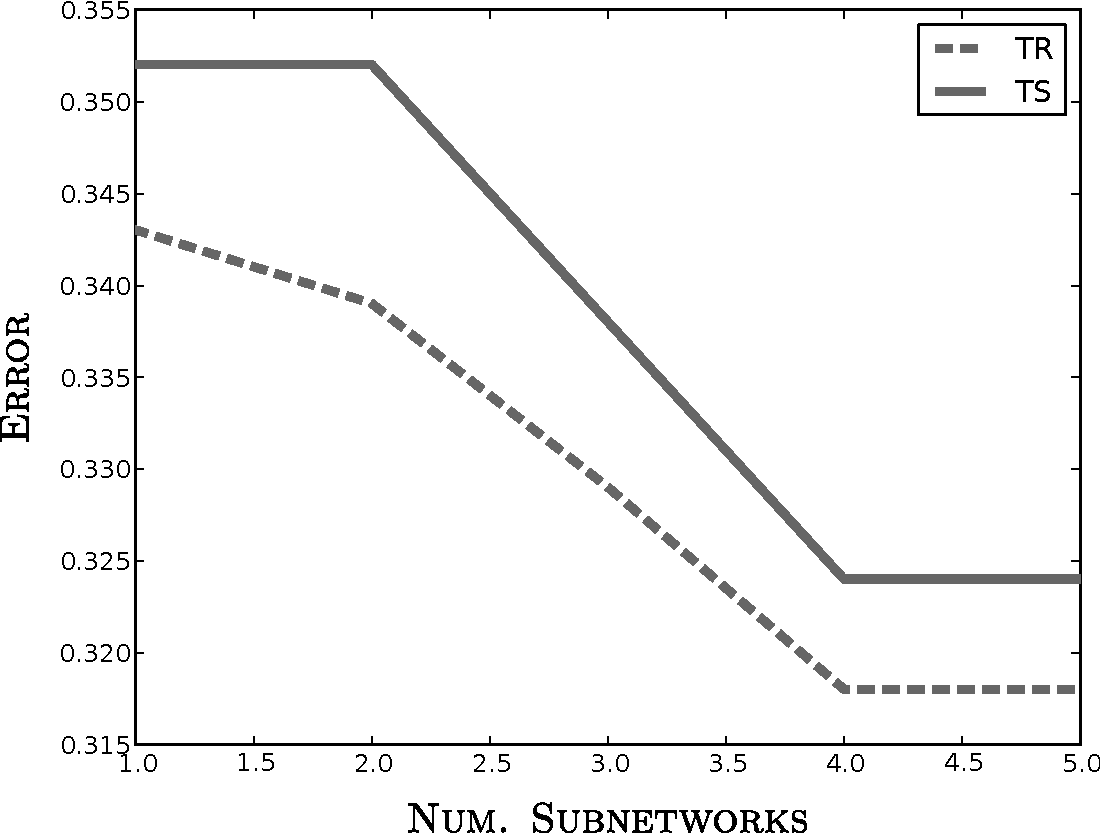
\includegraphics[width=0.5\columnwidth]{img/plot/ptc3}\\
\medskip
\caption[PTC: curve di apprendimento.]{GraphESN-FOF. Curve di apprendimento sul dataset PTC. Errore di misclassificazione commesso nel corso della costruzione della rete.\\
Linea tratteggiata: errore di training. Linea piena: errore di test.}
\label{fig:esperimenti:plot-ptc}
\end{figure}


L'accuratezza di predizione ottenuta tramite i modelli proposti risulta inoltre comparabile con quelle raggiunta applicando sugli stessi task dei modelli basati su kernel allo stato dell'arte nel trattamento dei domini strutturati \cite{Frohlich:OptimalAssignment}, riportati nella tabella~\ref{tab:esperimenti:kernelPTC}. Nel confronto è inoltre opportuno considerare che i modelli kernel-based prevedono, rispetto ai modelli proposti, l'impiego di maggiori risorse di calcolo ed operano attraverso l'impiego di metriche fissate a priori ed indipendenti dal task, in maniera simile a quanto avviene per i reservoir che non sfruttino output-feedback.
\begin{table}[tbp]
\small
\caption[Performance di metodi kernel-based su PTC]{Accuratezza media dei modelli e deviazione standard, in percentuale, di metodi basati su kernel applicati ai 4 task PTC.}
\label{tab:esperimenti:kernelPTC}
\centering
\begin{tabular}{l*{4}{c}}
\toprule
Method 	& FR	& FM	& MR	& MM	\\
\midrule
MG-Kernel & $70$ ($\pm 1$) & $65$ ($\pm 1$) & $63$ ($\pm 1$) & $69$ ($\pm 1$) \\
OA-Kernel & $70$ ($\pm 1$) & $65$ ($\pm 1$) & $63$ ($\pm 1$) & $68$ ($\pm 1$) \\
EM-Kernel & $69$ ($\pm 1$) & $65$ ($\pm 1$) & $61$ ($\pm 2$) & $67$ ($\pm 1$) \\
\bottomrule
\end{tabular}
\end{table}



%%%%%%%%%%%%%%%%%%%%%%%%%%%%%%%%%%%%%%
\subsection{Mutagenesis}
Le performance dei modelli sui tre task relativi al dataset Mutagenesis sono state calcolate ricorrendo ad una \emph{doppia k-fold cross-validation} (si veda il paragrafo~\ref{intro:validazione}) con un ciclo esterno di 10 fold ed un ciclo interno di 5 fold. La suddivisione del dataset è stata realizzata attraverso \emph{stratificazione} (si veda il paragrafo~\ref{intro:validazione}).
Per avere una stima più attendibile al variare dell'assegnazione iniziale dei pesi, 5 distinte ripetizioni sono state effettuate per ogni iperparametrizzazione testata.

Come nel caso di PTC, per ognuno dei modelli proposti sono state considerate due distinte configurazioni per la dimensione del reservoir delle sotto-reti: $N_R \in \lbrace 50, 30 \rbrace$. Il task structure-to-element di classificazione binaria, $N_Y = N_Z = 1$, prevede una dimensione delle etichette di input variabile, in base alla rappresentazione adottata: $N_U$ vale $11$, $13$, $15$ per AB, AB+C, AB+C+PS rispettivamente.

La soglia di convergenza del reservoir è stata fissata a $\epsilon = 10^{-5}$. Il coefficiente di contrazione $\sigma$ è stato in questo caso selezionato attraverso model selection.

Per interrompere la costruzione delle reti si è fissato $\delta_\textup{var} = 0.01$ e $\delta_\textup{tr} = 0.11$, riferito al miscalssification-rate. Come per PTC, il numero massimo di sotto-reti è stato fissato a $\delta_\textup{size} = 15$ nei casi in cui $N_R = 50$ e $\delta_\textup{size} = 20$ con $N_R = 30$.

Il learning-rate utilizzato per l'allenamento del readout globale tramite LMS è $\eta = 10^{-3}$.

La model selection è stata realizzata variando gli iperparametri $\lambda_\textup{in}$, $\lambda_\textup{fof}$, $\lambda_\textup{r}$,  $\lambda_\textup{wd}$ e $\sigma$, secondo i valori riportati nella tabella~\ref{tab:esperimenti:grigliaMutag}.
\begin{table}[tbp]
\small
\caption[Model selection: iperparametri per Mutagenesis]{Iperparametri usati per la model selection sui 3 task Mutagenesis.}
\label{tab:esperimenti:grigliaMutag}
\centering
\begin{tabular}{*{5}{c}}
\toprule
$\lambda_\textup{in}$ & $\lambda_\textup{fof}$ & $\lambda_\textup{r}$ & $\lambda_\textup{wd}$ & $\sigma$ \\
\midrule
$\lbrace 1.0, 0.1 \rbrace$ & $\lbrace 1.0, 2.0 \rbrace$ & $\lbrace 0.001, 0.01, 0.1 \rbrace$ & $\lbrace 0.0, 0.01 \rbrace$ &  $\lbrace 1.0, 2.0 \rbrace$\\
\bottomrule
\end{tabular}
\end{table}
Selezione e test del modello hanno dunque coinvolto, per i tre task e limitatamente ai casi costruttivi, l'allenamento di un totale di $72300$ diverse istanze di modello.

Sulle GraphESN la selezione degli iperparametri è stata eseguita facendo variare i valori di $N_R$, $\lambda_\textup{in}$, $\lambda_\textup{r}$ come indicato nella tabella~\ref{tab:esperimenti:grigliaMutagStandard}.
\begin{table}[tbp]
\small
\caption[Model selection: iperparametri per GraphESN su Mutag]{Iperparametri usati per la model selection di GraphESN sui 3 task Mutagenesis.}
\label{tab:esperimenti:grigliaMutagStandard}
\centering
\begin{tabular}{*{3}{c}}
\toprule
$N_R$ & $\lambda_\textup{in}$ & $\lambda_\textup{r}$ \\
\midrule
$\lbrace 500, 200, 100, 50 \rbrace$ & $\lbrace 1.0, 0.1 \rbrace$ & $\lbrace 0.01, 0.1, 0.2 \rbrace$ \\
\bottomrule
\end{tabular}
\end{table}

Nella tabella~\vref{tab:esperimenti:mutag} sono riportati i risultati sperimentali ottenuti sui tre task Mutagenesis.
I valori riportati rappresentano l'accuratezza percentuale di test (i.e.\ percentuale di grafi nel test-set classificata correttamente) mediata sulle $10$ fold e la deviazione standard media. Il dettaglio dei risultati sulle singole fold è riportato nelle tabelle~\ref{app:esp:Mutag-AB-CF}-\ref{app:esp:Mutag-ABCPC-FOF} (si veda l'appendice~\vref{app:esperimenti}).
\begin{table}[tbp]
\small
\caption[Accuratezza media su Mutagenesis]{Accuratezza media dei modelli e deviazione standard, in percentuale, sui 3 task Mutagenesis.}
\label{tab:esperimenti:mutag} 
\centering	
\begin{tabular}{l*{4}{c}}
\toprule
Model 		 & $N_R$& AB				  & AB+C			   & AB+C+PS	\\
\midrule
GraphESN 	 & 		& $75.2$ ($\pm 0.8$) & $76.5$ ($\pm 0.8$) & $80.3$ ($\pm 0.8$) \\
GraphESN-CF  & $50$ & $79.0$ ($\pm 2.3$) & $78.1$ ($\pm 1.8$) & $79.4$ ($\pm 0.5$) \\
GraphESN-CF  & $30$ & $79.6$ ($\pm 2.5$) & $76.0$ ($\pm 1.5$) & $79.7$ ($\pm 0.2$) \\
GraphESN-FW  & $50$ & $80.5$ ($\pm 2.8$) & $76.3$ ($\pm 2.0$) & $79.3$ ($\pm 1.8$) \\
GraphESN-FW  & $30$ & $79.7$ ($\pm 2.8$) & $76.7$ ($\pm 2.5$) & $80.6$ ($\pm 1.9$) \\
GraphESN-FOF & $50$ & $79.3$ ($\pm 3.6$) & $76.0$ ($\pm 2.8$) & $79.9$ ($\pm 1.9$) \\
GraphESN-FOF & $30$ & $76.8$ ($\pm 3.7$) & $77.0$ ($\pm 2.4$) & $80.0$ ($\pm 2.5$) \\
\bottomrule
\end{tabular}
\end{table}
Benché l'accuratezza nella predizione ottenuta dai modelli proposti risulti inferiore rispetto a quella raggiungibile con l'utilizzo di altri approcci (e.g.\ GNN \cite{Scarselli:GNN}), i risultati sperimentali evidenziano come i modelli costruttivi rappresentino una valida alternativa ed un miglioramento rispetto alle GraphESN.

Nella tabella~\ref{tab:dimensioni:mutag} sono riportati alcuni dati sulle dimensioni raggiunte delle reti nell'affrontare i tre task del dataset.
\begin{table}
\small
\caption[Dimensioni delle reti su Mutagenesis]{Numero di sotto-reti dei modelli sui tre task Mutagenesis. Numero massimo, numero minimo, media e moda.}
\label{tab:dimensioni:mutag} 
\centering	
\begin{tabular}{l*{4}{c}}
\toprule
Model 		 & Max & Min & Avg & Mode \\
\midrule
GraphESN-CF  & $17$ & $2$ & $3.9$ & $2$ \\
GraphESN-FW  & $15$ & $2$ & $4.6$ & $2$ \\
GraphESN-FOF & $18$ & $2$ & $5.5$ & $4$ \\
\bottomrule
\end{tabular}
\end{table}
In questo caso la tabella evidenzia la presenza di molte reti di dimensioni minime, suggerendo l'adozione di un criterio di stop più sofisticato per interrompere la costruzione della rete. La condizione di arresto utilizzata guarda infatti al solo errore di training commesso al passo precedente e, nel caso di task complessi, è ipotizzabile che questo possa non essere sufficiente a determinare l'effettivo andamento del processo di learning. Criteri di stop più sofisticati potrebbero, ad esempio, usare un validation-set per determinare la dimensione ottimale della rete.

La figura~\vref{fig:esperimenti:plot-mutag} mostra un esempio di alcune curve di apprendimento che caratterizzano l'applicazione dei modelli sul dataset. Il valore di errore indicato è il misclassification-rate. La figura evidenzia come l'errore di test diminuisca al decrescere dell'errore di training, e dunque come il processo di apprendimento costruttivo abbia effettivamente la capacità di migliorare la capacità predittiva del modello. Si riscontra tuttavia uno scostamento piuttosto ampio fra l'errore commesso sui dati training e quello commesso sui dati di test, che suggerisce l'opportunità di perfezionare i risultati ottenuti adottando ulteriori criteri di regolarizzazione, che riducano la complessità della rete.
\begin{figure}[p]
\centering
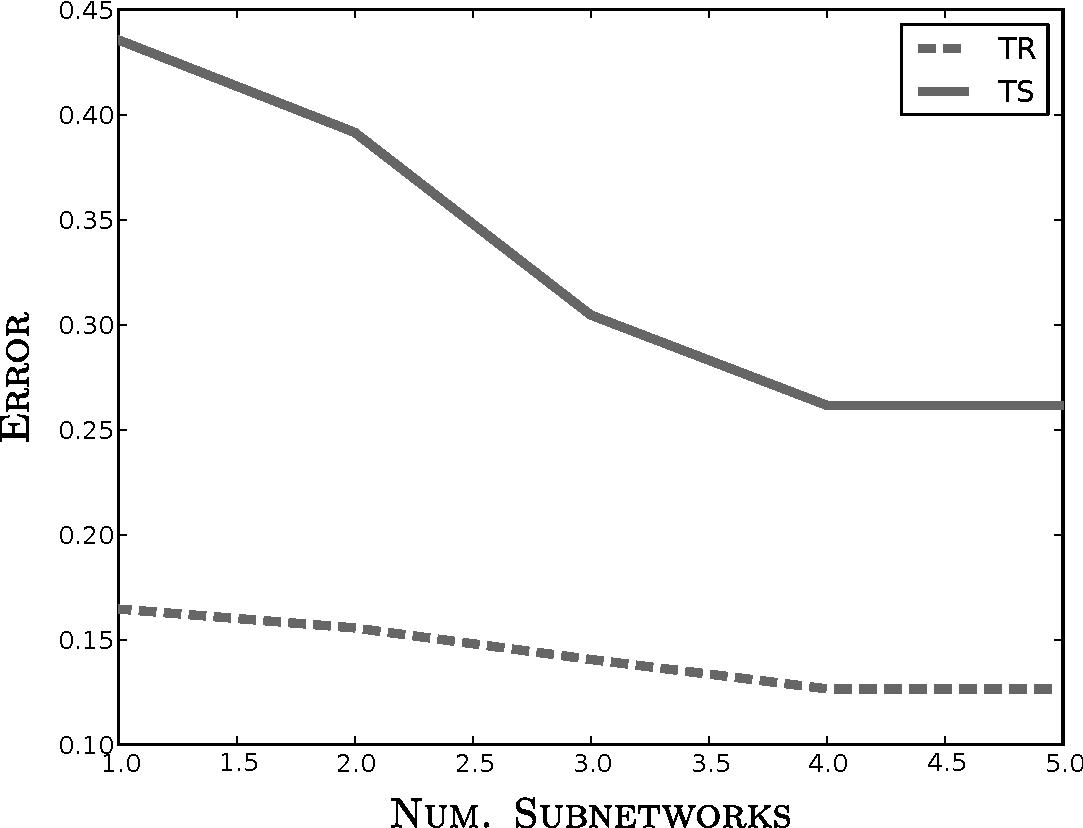
\includegraphics[width=0.5\columnwidth]{img/plot/mutag1}\\
\vspace*{0.8cm}
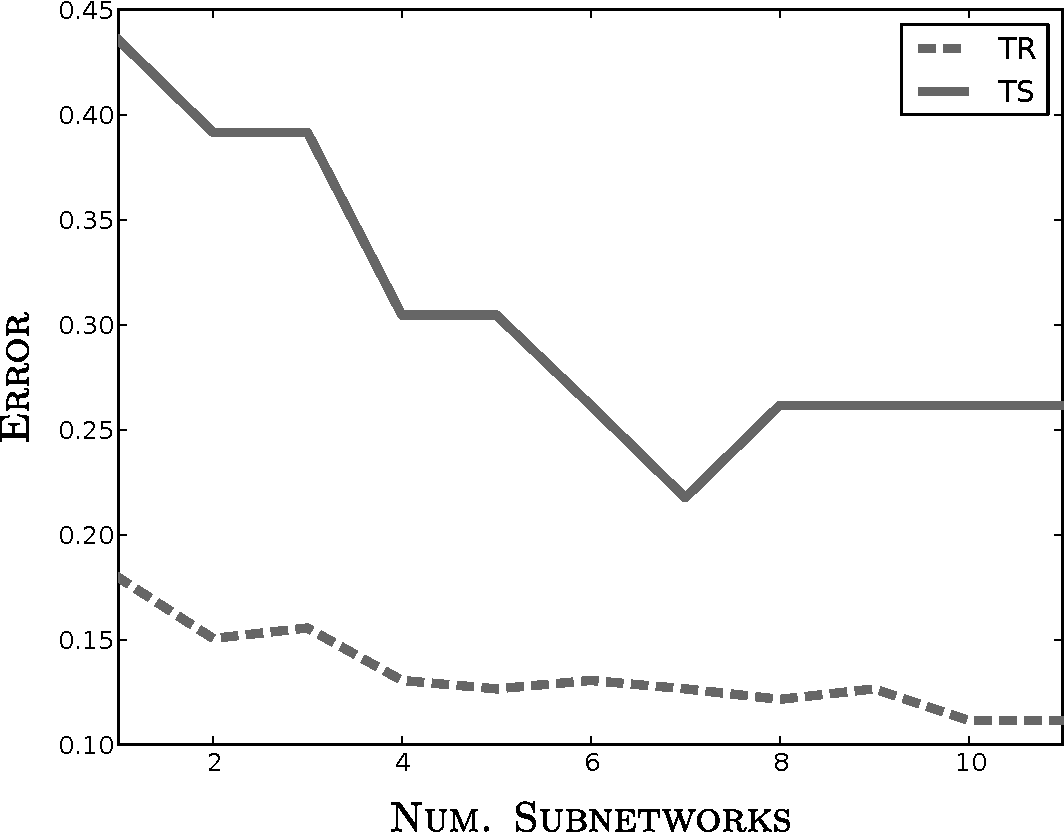
\includegraphics[width=0.5\columnwidth]{img/plot/mutag2}\\
\vspace*{0.8cm}
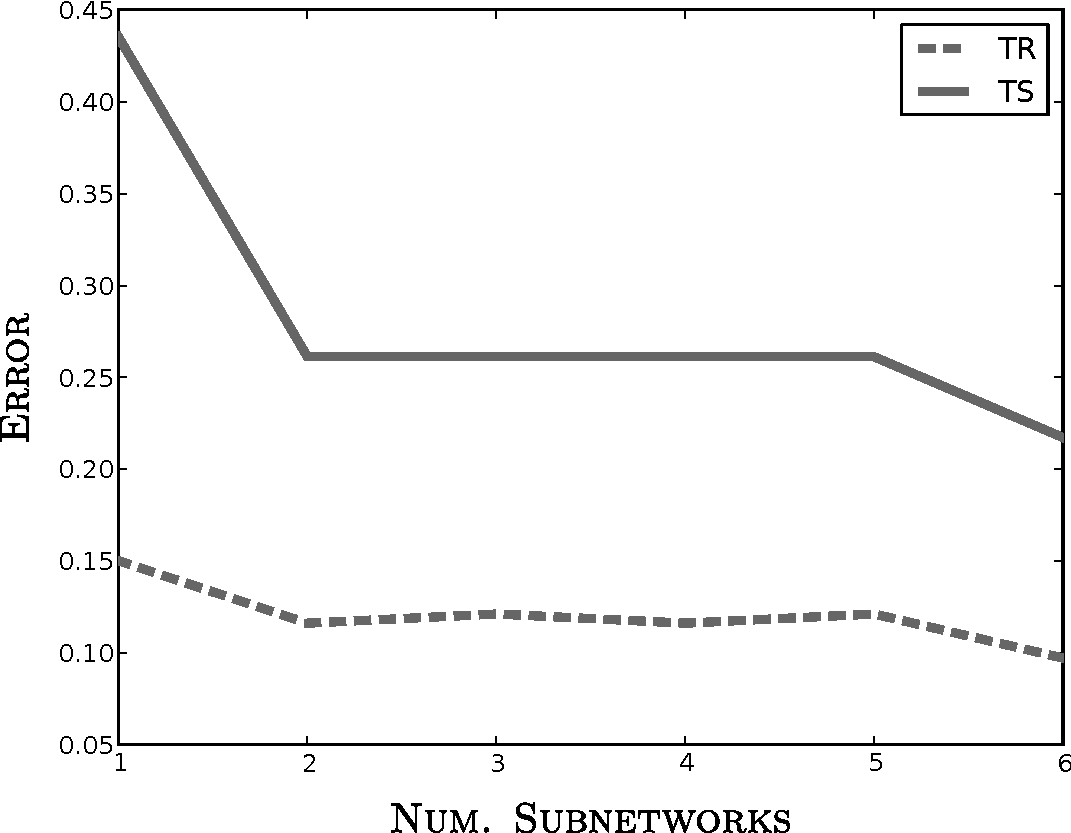
\includegraphics[width=0.5\columnwidth]{img/plot/mutag3}\\
\medskip
\caption[Mutag: curve di apprendimento.]{GraphESN-FOF. Curve di apprendimento sul dataset Mutagenesis. Errore di misclassificazione commesso nel corso della costruzione della rete.\\
Linea tratteggiata: errore di training. Linea piena: errore di test.}
\label{fig:esperimenti:plot-mutag}
\end{figure}

 

%%%%%%%%%%%%%%%%%%%%%%%%%%%%%%%%%%%%%%
\subsection{Bursi}
Sul dataset Bursi è stato possibile sfruttare una suddivisione preesistente del dataset in dati di training e dati di test. La selezione del modello è stata dunque realizzata suddividendo il training-set in $5$ fold tramite stratificazione e realizzando una \emph{k-fold cross-validation} con dei validation-set per selezionare gli iperparametri (si veda il paragrafo~\ref{intro:validazione}). Successivamente si è usato il partizionamento originale del dataset, in trainig-set e test-set, per testare le capacità predittive dei modelli. La suddivisione in fold è avvenuta ricorrendo a \emph{stratificazione} (si veda il paragrafo~\ref{intro:validazione}). Per ogni iperparametrizzazione testata sono state effettuate 5 ripetizioni distinte, in modo da variare l'assegnazione iniziale dei pesi.

Sul dataset sono stati testati modelli costruttivi con sotto-reservoir di dimensione $N_R = 100$. Il task structure-to-element di classificazione binaria $N_Y = N_Z = 1$ prevede una dimensione delle etichette di input $N_U = 14$.

La soglia di convergenza del reservoir utilizzata è $\epsilon = 10^{-5}$, mentre il coefficiente di contrazione è stato fissato a $\sigma = 1.0$.

Per interrompere la costruzione delle reti si è fissato $\delta_\textup{var} = 0.01$ e $\delta_\textup{tr} = 0.15$, riferito al miscalssification-rate, con un numero massimo di sotto-reti consentito $\delta_\textup{size} = 10$.

Il learning-rate $\eta = 10^{-3}$ è stato utilizzato per l'allenamento del readout globale tramite LMS.

Data la dimensione del dataset, ed il relativo onere computazionale, la model selection su Bursi ha interessato i soli iperparametri $\lambda_\textup{fof}$ e $\lambda_\textup{r}$, mantenendo fissi i parametri $\lambda_\textup{wd} = 0$ per l'apprendimento nel readout globale e $\lambda_\textup{in} = 1.0$ per lo scaling dei pesi dall'input.
I valori degli iperparametri coinvolti nella model selection sono riportati nella tabella~\ref{tab:esperimenti:grigliaBursi}.
\begin{table}[tbp]
\small
\caption[Model selection: iperparametri per Bursi]{Iperparametri usati per la model selection su Bursi.}
\label{tab:esperimenti:grigliaBursi}
\centering
\begin{tabular}{*{2}{c}}
\toprule
$\lambda_\textup{fof}$ & $\lambda_\textup{r}$ \\
\midrule
$\lbrace 1.0, 2.0 \rbrace$ & $\lbrace 0.0, 0.001, 0.01, 0.1 \rbrace$ \\
\bottomrule
\end{tabular}
\end{table}
%
Le performance su GraphESN sono invece state calcolate facendo variare i parametri $N_R$ e $\lambda_\textup{r}$ in accordo ai valori riportati nella tabella~\ref{tab:esperimenti:grigliaBursiStandard}.
\begin{table}[tbp]
\small
\caption[Model selection: iperparametri per GraphESN su Bursi]{Iperparametri usati per la model selection di GraphESN su Bursi.}
\label{tab:esperimenti:grigliaBursiStandard}
\centering
\begin{tabular}{*{2}{c}}
\toprule
$N_R$ & $\lambda_\textup{r}$ \\
\midrule
$\lbrace 500, 200, 100 \rbrace$ & $\lbrace 0.0, 0.001, 0.01, 0.1 \rbrace$ \\
\bottomrule
\end{tabular}
\end{table}
%
Gli esperimenti sul dataset hanno dunque richiesto l'allenamento complessivo di $680$ diverse reti.

I risultati sperimentali ottenuti sono riportati nella tabella~\ref{tab:esperimenti:bursi}, con i valori ad indicare l'accuratezza percentuale e la deviazione standard riscontrate nel classificare i dati sia di training che di test.
\begin{table}[tbp]
\small
\caption[Accuratezza media su Bursi]{Accuratezza media in training e test dei modelli e deviazione standard, in percentuale, sul dataset Bursi.}
\label{tab:esperimenti:bursi} 
\centering	
\begin{tabular}{l*{3}{c}}
\toprule
Model           & $N_R$     & TR                    & TS        \\
\midrule
GraphESN        &           & $77.9$ ($\pm 0.2$)    & $76.2$ ($\pm 0.2$) \\
GraphESN-CF     & $100$     & $78.3$ ($\pm 0.4$)    & $76.7$ ($\pm 0.7$) \\
GraphESN-FW     & $100$     & $78.4$ ($\pm 0.8$)    & $77.1$ ($\pm 0.7$) \\
GraphESN-FOF    & $100$     & $79.8$ ($\pm 0.5$)    & $78.0$ ($\pm 0.9$) \\
\bottomrule
\end{tabular}
\end{table}
Dai dati emerge come in questo caso l'approccio costruttivo permetta di superare sistematicamente le performance predittive ottenute tramite GraphESN. Risulta inoltre come il miglioramento delle performance segua l'arricchimento della connettività progressivo realizzato dai tre modelli costruttivi.

La tabella~\ref{tab:dimensioni:mutag} riporta i dati sulle dimensioni raggiunte delle reti nell'affrontare il task.
\begin{table}
\small
\caption[Dimensioni delle reti su Bursi]{Numero di sotto-reti dei modelli su Bursi. Numero massimo, numero minimo, media e moda.}
\label{tab:dimensioni:bursi} 
\centering	
\begin{tabular}{l*{4}{c}}
\toprule
Model 		 & Max & Min & Avg & Mode \\
\midrule
GraphESN-CF  & $5$ & $2$ & $3.2$ & $2$ \\
GraphESN-FW  & $8$ & $2$ & $4.2$ & $4$ \\
GraphESN-FOF & $10$ & $4$ & $6.8$ & $7$ \\
\bottomrule
\end{tabular}
\end{table}
Si nota come il modello GraphESN-FOF riesca a procedere più a lungo nella costruzione della rete, probabilmente grazie ad una maggiore capacità di fitting che permette all'errore sul trainig-set di variare maggiormente, senza determinare l'interruzione del processo di costruzione della rete.

La figura~\vref{fig:esperimenti:plot-bursi} mostra un esempio dell'andamento del training di una rete di tipo GraphESN-FOF applicata al dataset, evidenziando il progresso della capacità predittiva della rete nel corso del procedimento di costruzione della rete.
\begin{figure}[p]
\centering
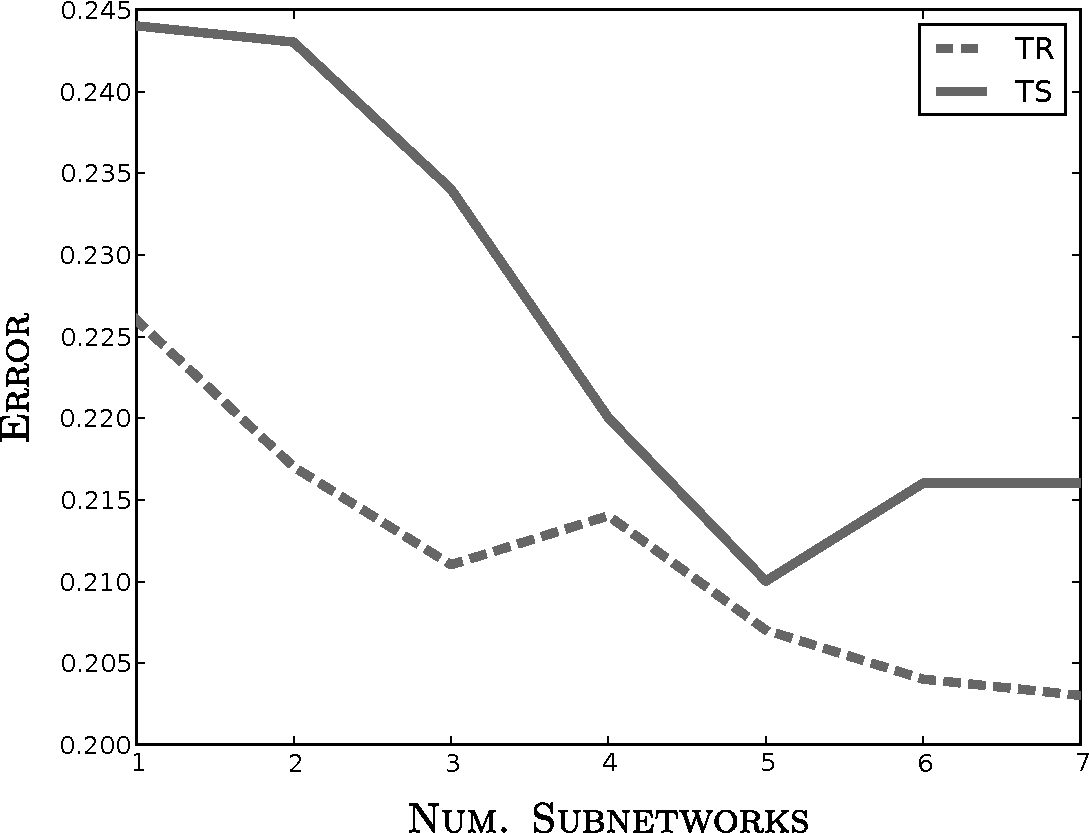
\includegraphics[width=0.7\columnwidth]{img/plot/bursi}
\medskip
\caption[Bursi: curve di apprendimento.]{GraphESN-FOF. Curve di apprendimento sul dataset Bursi. Errore di misclassificazione commesso nel corso della costruzione della rete.\\
Linea tratteggiata: errore di training. Linea piena: errore di test.}
\label{fig:esperimenti:plot-bursi}
\end{figure}


%%%%%%%%%%%%%%%%%%%%%%%%%%%%%%%%%%%%%%
\subsection{Angiotensin Converting Enzyme}
Sul dataset ACE non è stato svolto un processo di selezione degli iperparametri ottimali dei modelli, limitando l'analisi sperimentale ad una singola iperparametrizzazione, scelta sulla base di valutazioni empiriche. La valutazione della performance del modello è stata svolta attraverso \emph{k-fold cross-validation} su $10$ fold (si veda il paragrafo~\ref{intro:validazione}), ripetendo il test $5$ volte in modo da variare l'inizializzazione dei pesi di reservoir.

Il dataset ACE ha permesso di applicare i modelli ad un task structure-to-element di regressione, con $N_Y = N_Z = 1$. Le etichette associate ai vertici dell'input risultano avere dimensione $N_U = 8$.

Per interrompere il processo di encoding è stata usata la soglia $\epsilon = 10^{-5}$, fissando un coefficiente di contrazione per ogni reservoir $\sigma = 1.0$.

Il processo di costruzione della rete è stato interrotto fissando $\delta_\textup{var} = 0.01$ e senza tenere conto di alcun errore minimo sul training-set, $\delta_\textup{tr} = -1.0$, con un numero massimo di sotto-reti consentito pari a $\delta_\textup{size} = 30$.

L'allenamento del readout globale è stato svolto attraverso LMS con learning-rate $\eta = 10^{-3}$ e senza applicare alcun fattore di weight-decay, $\lambda_\textup{wd} = 0$.
L'apprendimento nelle sotto-reti è stato realizzato attraverso una Ridge Regression con fattore di regolarizzazione $\lambda_\textup{r} = 0.1$.

Per l'inizializzazione dei pesi sono stati fissati i parametri $\lambda_\textup{in} = 1.0$ e $\lambda_\textup{fof} = 2.0$. 
Il test è stato svolto utilizzando sotto-reti di dimensione $N_R = 30$.

Per poter effettuare un confronto, l'allenamento su GraphESN è stato eseguito mantenendo, laddove abbia un senso, la stessa iperparametrizzazione usata per i modelli costruttivi. La dimensione del reservoir in questo caso è però stata fatta variare $N_R \in \lbrace 90, 150, 300, 450 \rbrace$. Nel seguito viene riportato solo il risultato migliore ottenuto (i.e.\ $N_R = 300$), in termini di performance predittiva.

La tabella~\ref{tab:esperimenti:ACE} mostra i risultati sperimentali ottenuti, indicando l'errore quadratico medio e la deviazione standard mediati sulle $10$ fold.
\begin{table}[tb]
\small
\caption[Accuratezza media su ACE]{Errore quadratico medio in training e test dei modelli e deviazione standard sul dataset ACE.}
\label{tab:esperimenti:ACE}
\centering
\begin{tabular}{l*{2}{c}}
\toprule
Model & MSE (TR) & MSE (TS) \\
\midrule
GraphESN    & $1.83$ ($\pm 0.01$) &	$2.13$ ($\pm 0.03$) \\ 
GraphESN-CF & $2.03$ ($\pm 0.07$) & $2.37$ ($\pm 0.15$) \\
GraphESN-FW & $1.71$ ($\pm 0.02$) & $2.02$ ($\pm 0.06$) \\
GraphESN-FOF & $1.60$ ($\pm 0.07$) & $2.03$ ($\pm 0.06$) \\
\bottomrule
\end{tabular}
\end{table}
%
Benché non sia stata effettuata una selezione rigorosa degli iperparametri ottimali per il task, è importante sottolineare come i risultati ottenuti siano comparabili con quelli riportati in letteratura relativamente all'applicazione di altri modelli per l'apprendimento di trasduzioni strutturali.
La tabella~\ref{tab:esperimenti:kernelACE} indica le performance su ACE ottenute attraverso modelli basati su kernel allo stato dell'arte nel trattamento di domini strutturati \cite{Hinselmann:GraphKernels}.
\begin{table}[tbp]
\small
\caption[Performance di metodi kernel-based su ACE]{Errore quadratico medio dei modelli e deviazione standard di metodi basati su kernel sul dataset ACE.}
\label{tab:esperimenti:kernelACE}
\centering
\begin{tabular}{lc}
\toprule
Kernel 	& MSE \\
\midrule
DotProduct & $1.60$ ($\pm 0.59$) \\
2D-LAP(CK) & $1.67$ ($\pm 0.63$) \\
2D-LAP(OA) & $1.81$ ($\pm 0.65$) \\
3D-LAP(CK) & $2.04$ ($\pm 0.78$) \\
3D-LAP(OA) & $1.91$ ($\pm 0.71$) \\
XD-LAP(CK) & $1.90$ ($\pm 0.71$) \\
XD-LAP(OA) & $1.99$ ($\pm 0.71$) \\
MACCS keys & $2.02$ ($\pm 0.69$) \\
Marginalized GK & $1.74$ ($\pm 0.72$) \\
Pharmacophore & $2.24$ ($\pm 0.82$) \\
OAK & $1.49$ ($\pm 0.68$) \\
Tanimoto DFS & $1.85$ ($\pm 0.64$) \\
\bottomrule
\end{tabular}
\end{table}

La figura~\vref{fig:esperimenti:plot-ace} riporta una campione delle curve di apprendimento ottenute utilizzando una rete di tipo GraphESN-FOF sul dataset. I grafici dimostrano l'efficacia del processo di apprendimento, mostrando tuttavia come la mancanza della scelta di un setting specifico su ogni fold risulti in un comportamento non uniforme dei modelli sulle varie fold.
\begin{figure}[p]
\centering
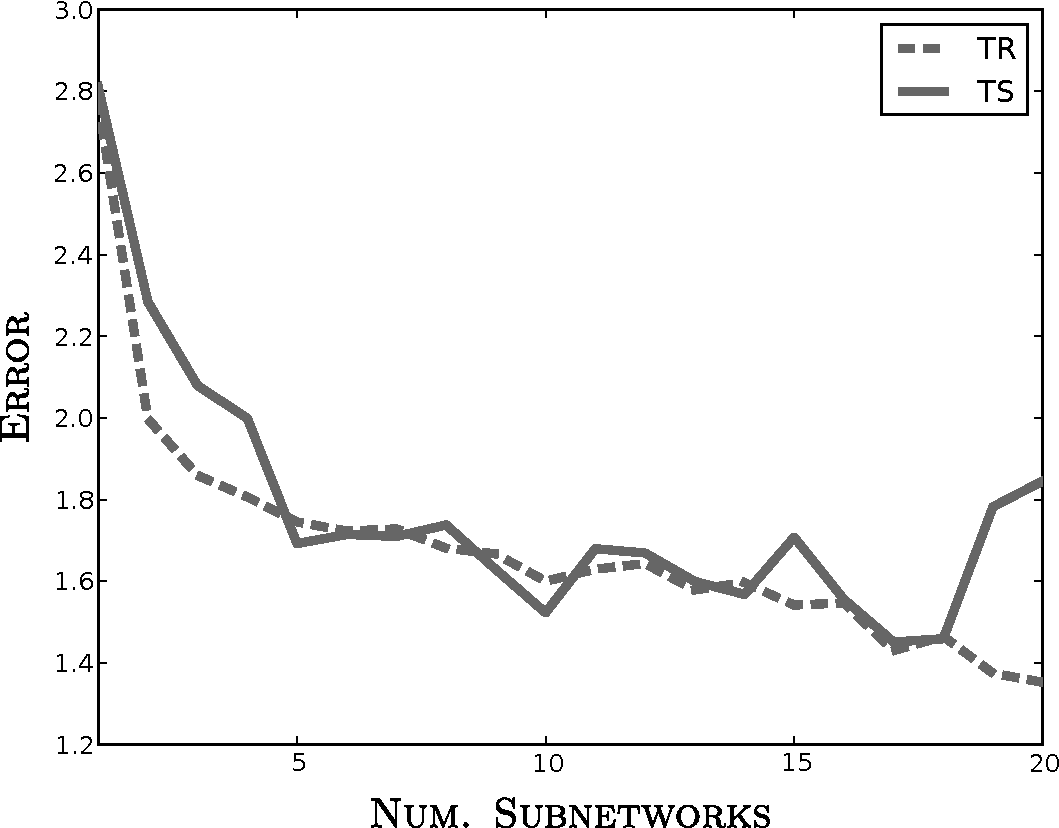
\includegraphics[width=0.5\columnwidth]{img/plot/ace1}\\
\vspace*{0.8cm}
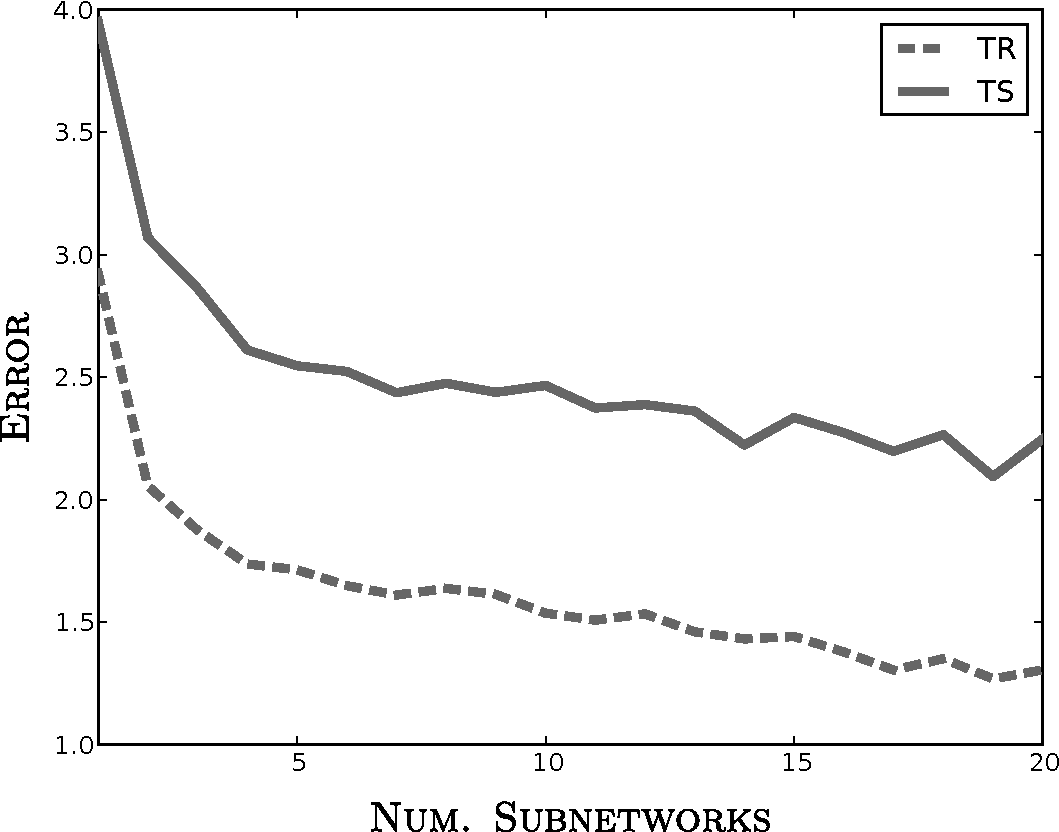
\includegraphics[width=0.5\columnwidth]{img/plot/ace2}\\
\vspace*{0.8cm}
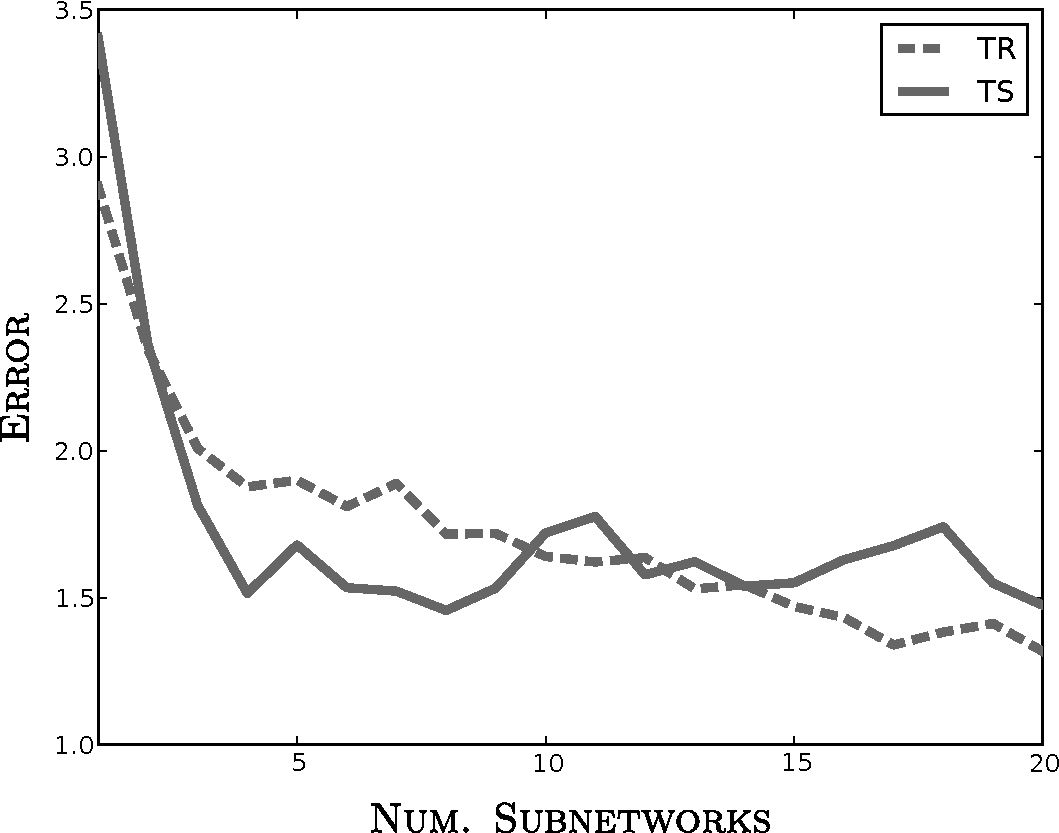
\includegraphics[width=0.5\columnwidth]{img/plot/ace3}\\
\medskip
\caption[ACE: curve di apprendimento.]{GraphESN-FOF. Curve di apprendimento sul dataset ACE. Errore quadratico medio (MSE) commesso nel corso della costruzione della rete.\\
Linea tratteggiata: errore di training. Linea piena: errore di test.}
\label{fig:esperimenti:plot-ace}
\end{figure}


%%%%%%%%%%%%%%%%%%%%%%%%%%%%%%%%%%%%%%
\section{Considerazioni}\label{sec:esperiment:considerazioni}
Guardando ai risultati emerge piuttosto chiaramente come la strategia costruttiva, seppur meno onerosa dal punto di vista computazionale, possa rappresentare un potenziamento delle GraphESN. Sia la fase di training che la selezione del modello si avvalgono infatti dell'approccio costruttivo per ridurre il costo computazionale senza che questo determini una perdita nella capacità predittiva della rete: i risultati ottenuti mostrano infatti come i modelli proposti siano in grado di superare nella maggior parte dei casi le performance raggiunte da GraphESN, raggiungendo risultati comparabili negli altri casi. In quest'ottica i modelli introdotti si configurano come uno strumento utile nel trattamento dei domini strutturati, in grado di soddisfare efficacemente i vincoli imposti dalla presenza di risorse di calcolo o di tempo limitate.

Guardando alla sola analisi delle performance, tuttavia, alcune caratteristiche dei modelli proposti rimangono poco chiare. Si nota ad esempio come l'introduzione e lo sfruttamento di un meccanismo stabile di output-feedback, nel modello GraphESN-FOF, non corrisponda ad un miglioramento sistematico dell'accuratezza predittiva della rete. Ulteriori analisi sperimentali hanno tuttavia permesso di verificare l'effetto dei segnali di output-feedback sui reservoir delle sotto-reti.
L'organizzazione dello spazio degli stati dei reservoir è stata investigata attraverso la Principal Component Analysis (PCA) \cite{Jolliffe:PCA}. La figura~\vref{fig:esperimenti:pca-ptc-fof} mostra le prime due componenti principali dello spazio degli stati dei reservoir di sotto-reti appartenenti ad una GraphESN-FOF. I punti dei plot corrispondono ai grafi in input, colorati in base al target loro assegnato e disposti nello spazio delle features secondo l'encoding corrispondente. Lo stesso procedimento e lo stesso setting sperimentale sono stati utilizzati per realizzare la figura~\vref{fig:esperimenti:pca-ptc-nofof}, che mostra lo spazio degli stati dei reservoir di una rete di tipo GraphESN-CF, in cui non sono presenti connessioni di output-feedback. Dal confronto delle due figure emerge chiaramente come il meccanismo di output-feedback abbia l'effetto di modificare le dinamiche del processo di encoding, organizzando gli input nello spazio degli stati in maniera coerente con il task affrontato ed aumentando progressivamente la distanza fra input appartenenti a classi distinte. 
%
\begin{figure}[p]
\centering
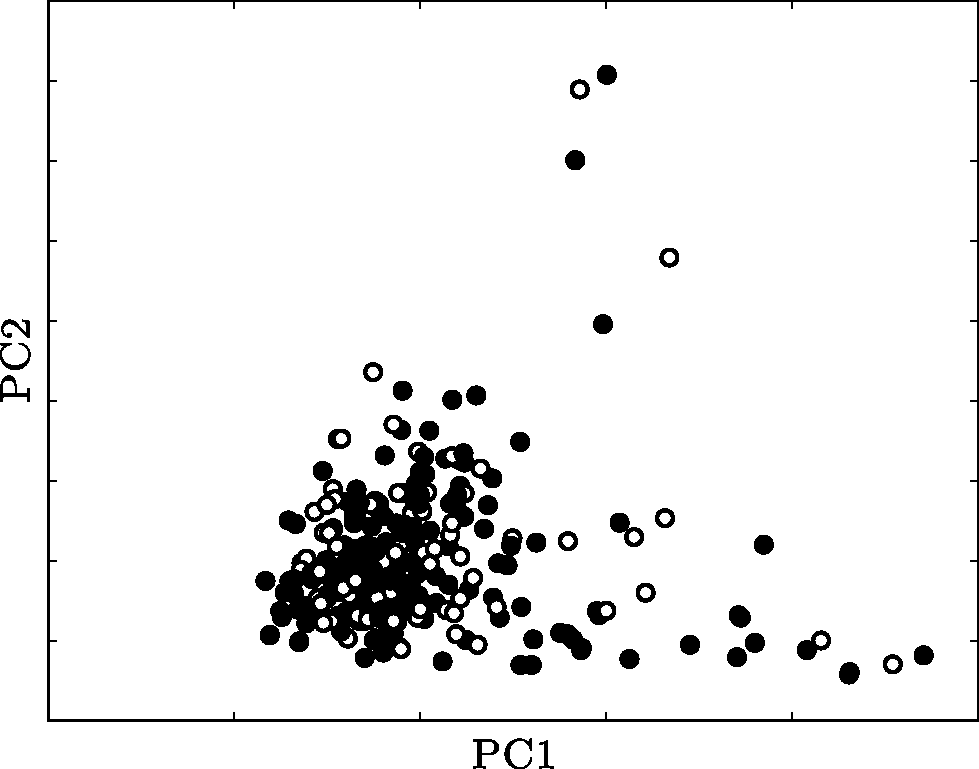
\includegraphics[width=0.5\columnwidth]{img/pca/pca-ptc-fof1}\\
\vspace*{0.8cm}
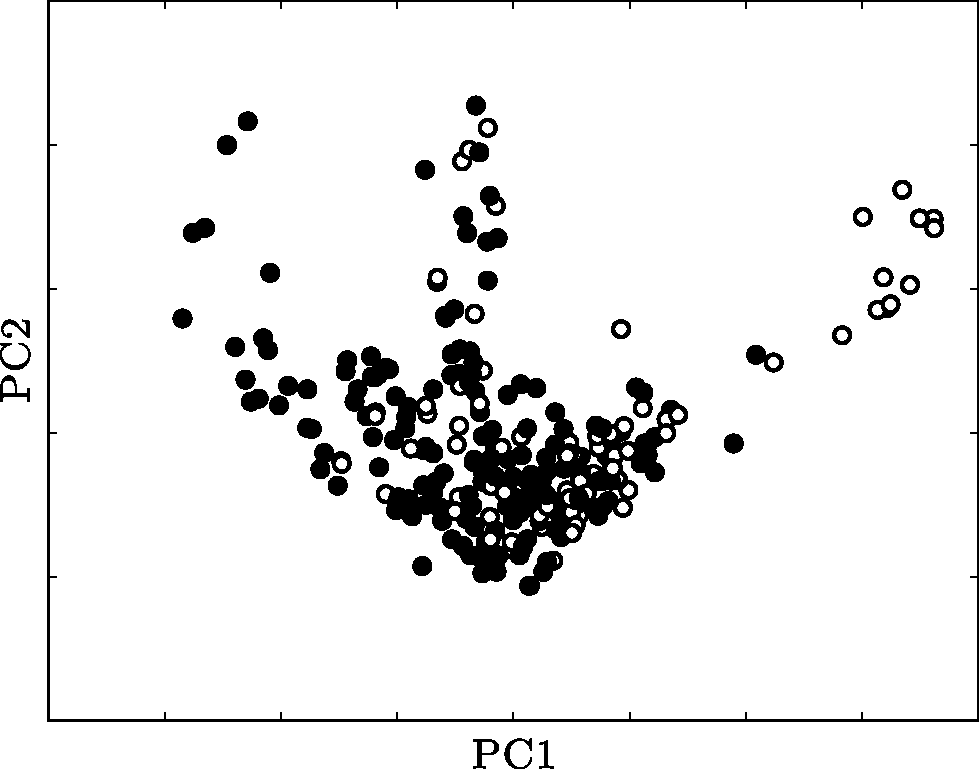
\includegraphics[width=0.5\columnwidth]{img/pca/pca-ptc-fof2}\\
\vspace*{0.8cm}
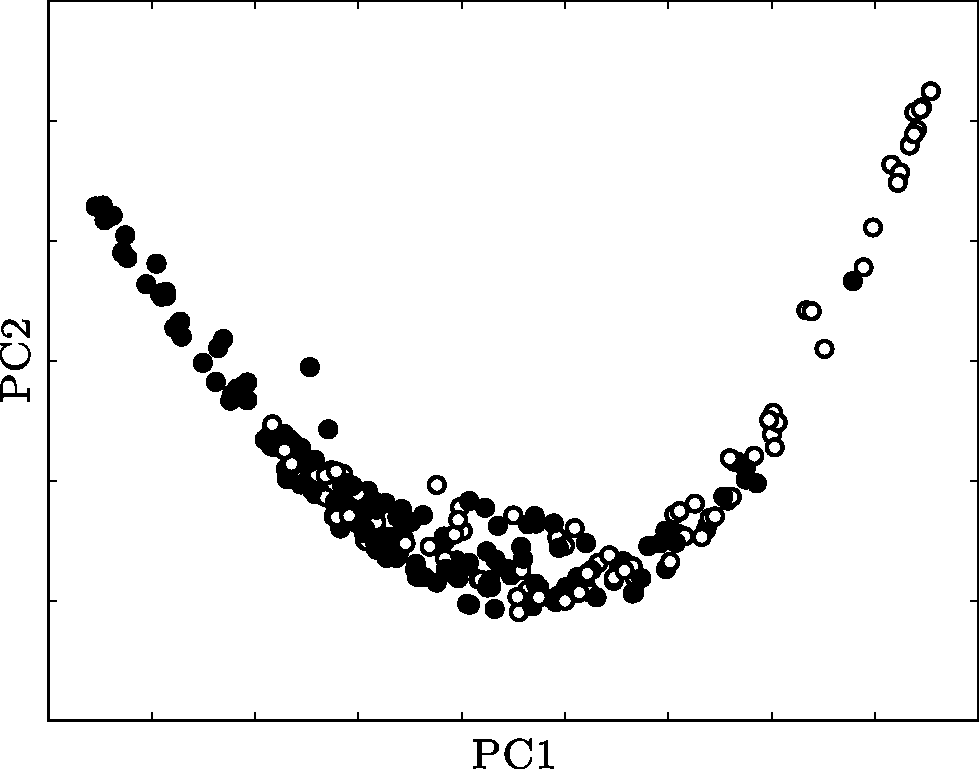
\includegraphics[width=0.5\columnwidth]{img/pca/pca-ptc-fof3}\\
\medskip
\caption[PCA dei reservoir. GraphESN-FOF su PTC-FR.]{Plot delle prime due componenti principali dello spazio degli stati dei reservoir nelle sotto-reti. Modello GraphESN-FOF applicato al task PTC-FR.\\ 
In nero: gli input con target $-1$. In bianco: gli input con target $+1$.\\
Reservoir riportati: (\emph{alto}) sotto-rete 1; (\emph{centro}) sotto-rete 5; (\emph{basso}) sotto-rete 9.}
\label{fig:esperimenti:pca-ptc-fof}
\end{figure}
%
\begin{figure}[p]
\centering
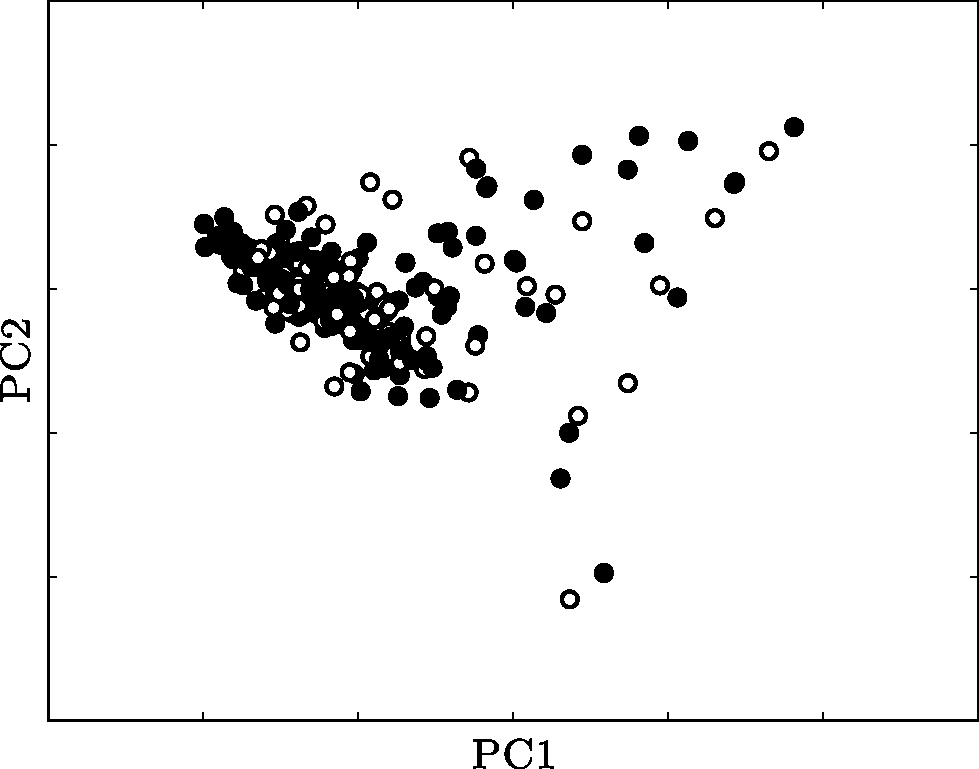
\includegraphics[width=0.5\columnwidth]{img/pca/pca-ptc-nofof1}\\
\vspace*{0.8cm}
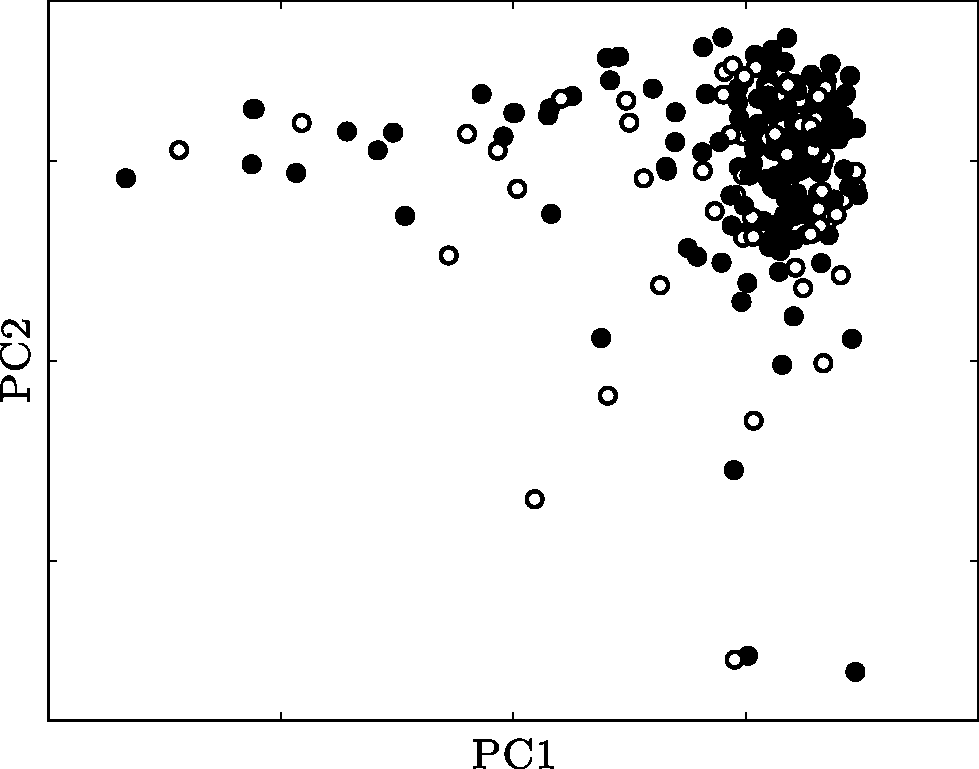
\includegraphics[width=0.5\columnwidth]{img/pca/pca-ptc-nofof2}\\
\vspace*{0.8cm}
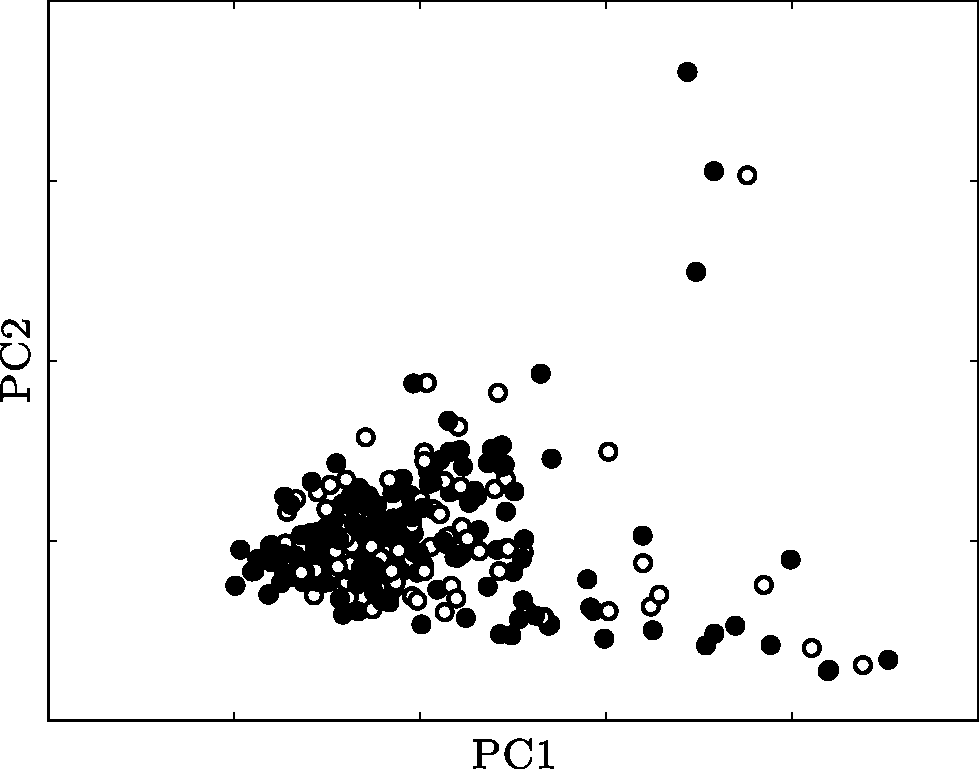
\includegraphics[width=0.5\columnwidth]{img/pca/pca-ptc-nofof3}\\
\medskip
\caption[PCA dei reservoir. GraphESN-CF su PTC-FR.]{Plot delle prime due componenti principali dello spazio degli stati dei reservoir nelle sotto-reti. Modello GraphESN-CF applicato al task PTC-FR.\\ 
In nero: gli input con target $-1$. In bianco: gli input con target $+1$.\\
Reservoir riportati: (\emph{alto}) sotto-rete 1; (\emph{centro}) sotto-rete 4; (\emph{basso}) sotto-rete 8.}
\label{fig:esperimenti:pca-ptc-nofof}
\end{figure}
%
\\
L'analisi della PCA è stata ripetuta sul dataset ACE, corrispondente ad un task di regressione. La figura~\vref{fig:esperimenti:pca-ace-fof} mostra lo spazio degli stati di una rete GraphESN-FOF, mentre la figura~\ref{fig:esperimenti:pca-ace-nofof} si riferisce ad una rete GraphESN-CF con lo stesso setting. Gli input sono in questo caso colorati in scale di grigio in accordo al valore target corrispondente, che varia in un intervallo continuo.
Anche in questo caso le figure evidenziano come la presenza di output-feedback abbia l'effetto di organizzare la rappresentazione dell'input all'interno dello spazio degli stati in maniera consistente con il task. Al contrario, nei due casi visti, l'assenza di output-feedback fa sì che i reservoir delle varie sotto-reti si comportino in maniera sostanzialmente simile l'uno all'altro, con variazioni dell'encoding che dipendono unicamente dalla diversa inizializzazione random dei pesi sulle connessioni ricorrenti.\\
Dall'analisi della PCA sugli stati dei reservoir risulta quindi ben evidente come la presenza degli output-feedback introduca effettivamente dell'informazione supervisionata all'interno di reservoir non adattivi.
%
\begin{figure}[p]
\centering
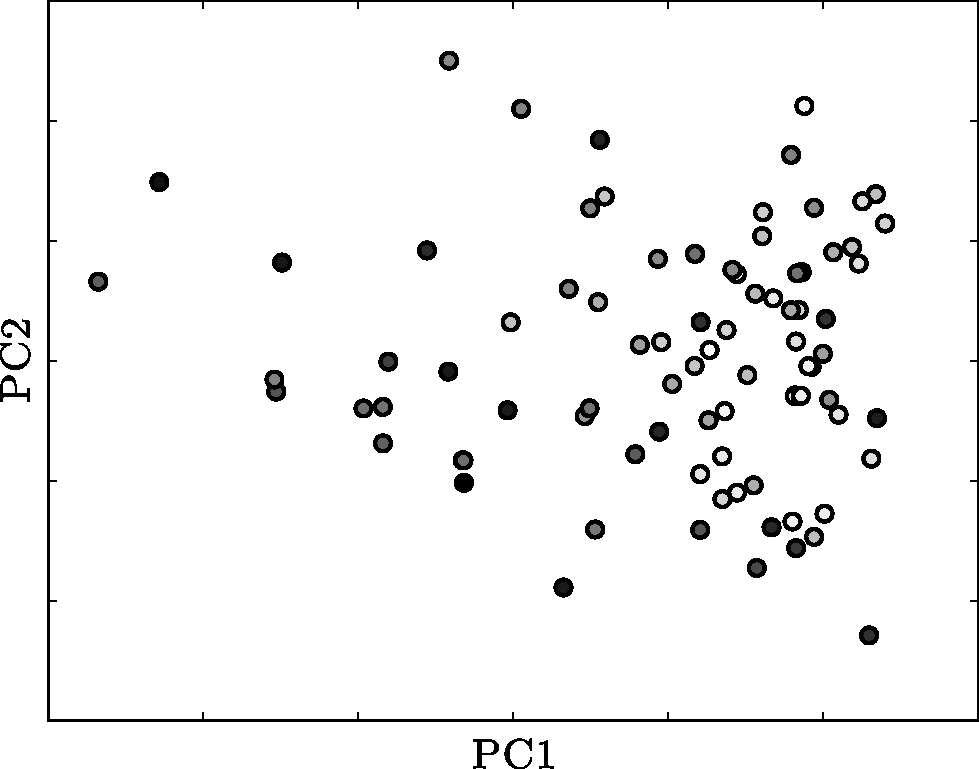
\includegraphics[width=0.5\columnwidth]{img/pca/pca-ace-fof1}\\
\vspace*{0.8cm}
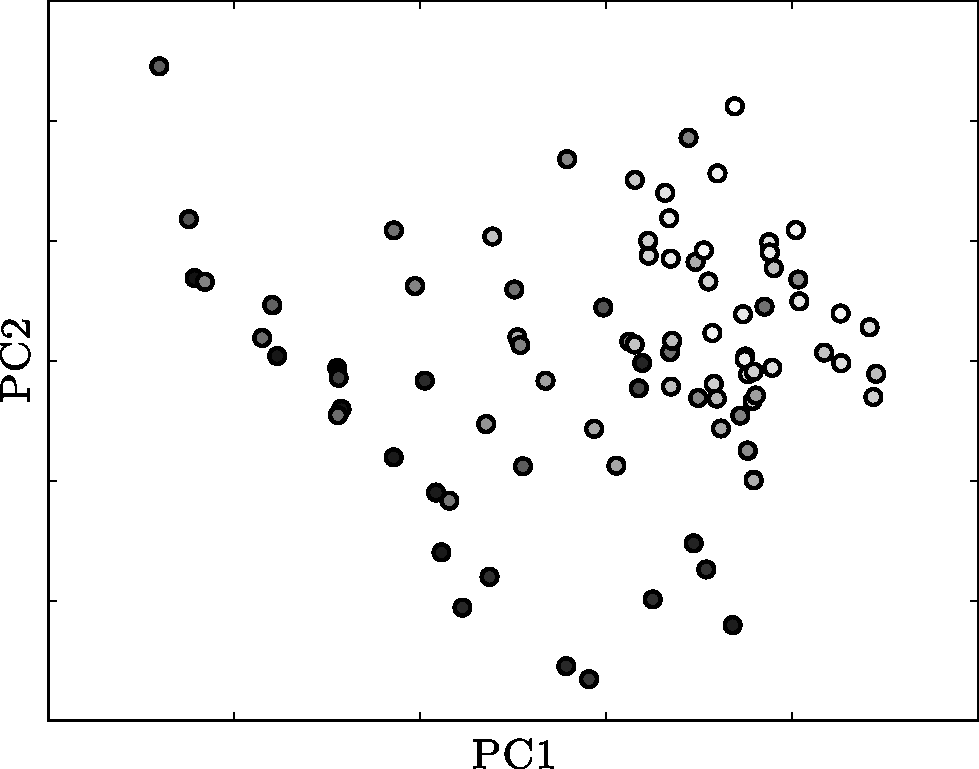
\includegraphics[width=0.5\columnwidth]{img/pca/pca-ace-fof2}\\
\vspace*{0.8cm}
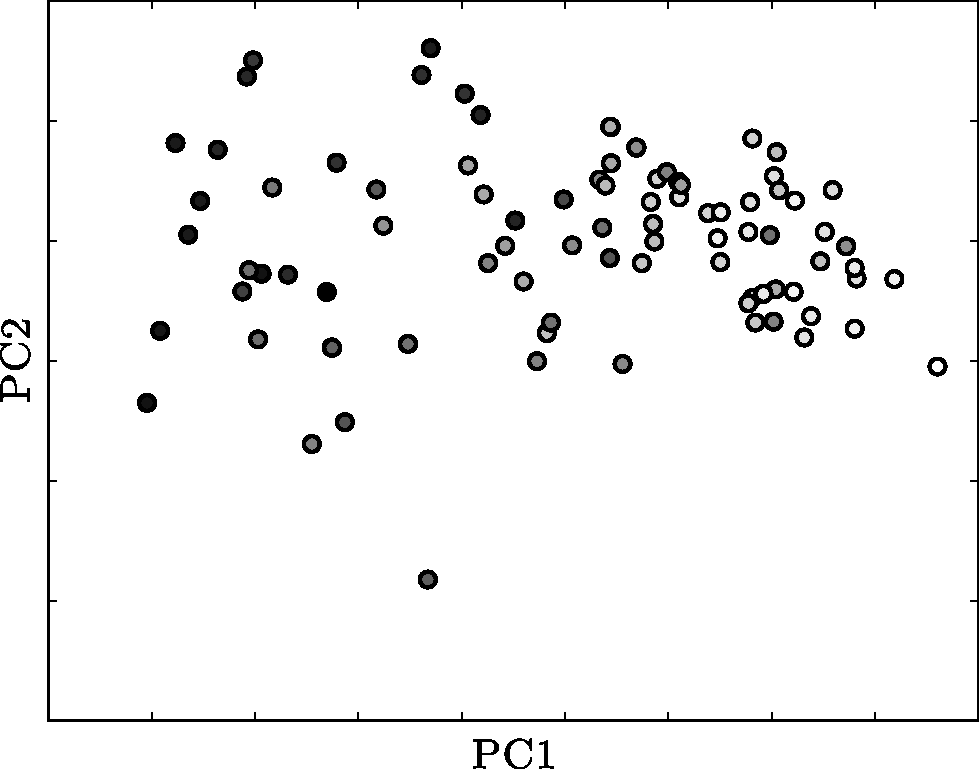
\includegraphics[width=0.5\columnwidth]{img/pca/pca-ace-fof3}\\
\medskip
\caption[PCA dei reservoir. GraphESN-FOF su ACE.]{Plot delle prime due componenti principali dello spazio degli stati dei reservoir nelle sotto-reti. Modello GraphESN-FOF applicato al task ACE.\\ 
In scuro gli input con valori target più alti.\\
Reservoir riportati: (\emph{alto}) sotto-rete 1; (\emph{centro}) sotto-rete 4; (\emph{basso}) sotto-rete 9.}
\label{fig:esperimenti:pca-ace-fof}
\end{figure}
%
\begin{figure}[p]
\centering
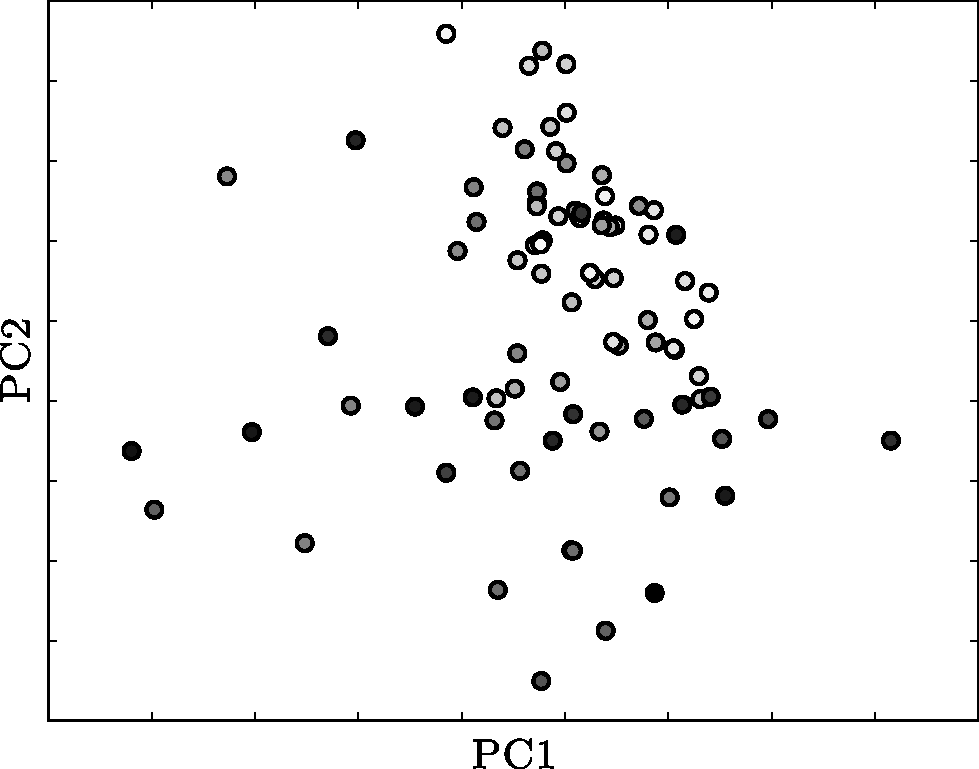
\includegraphics[width=0.5\columnwidth]{img/pca/pca-ace-nofof1}\\
\vspace*{0.8cm}
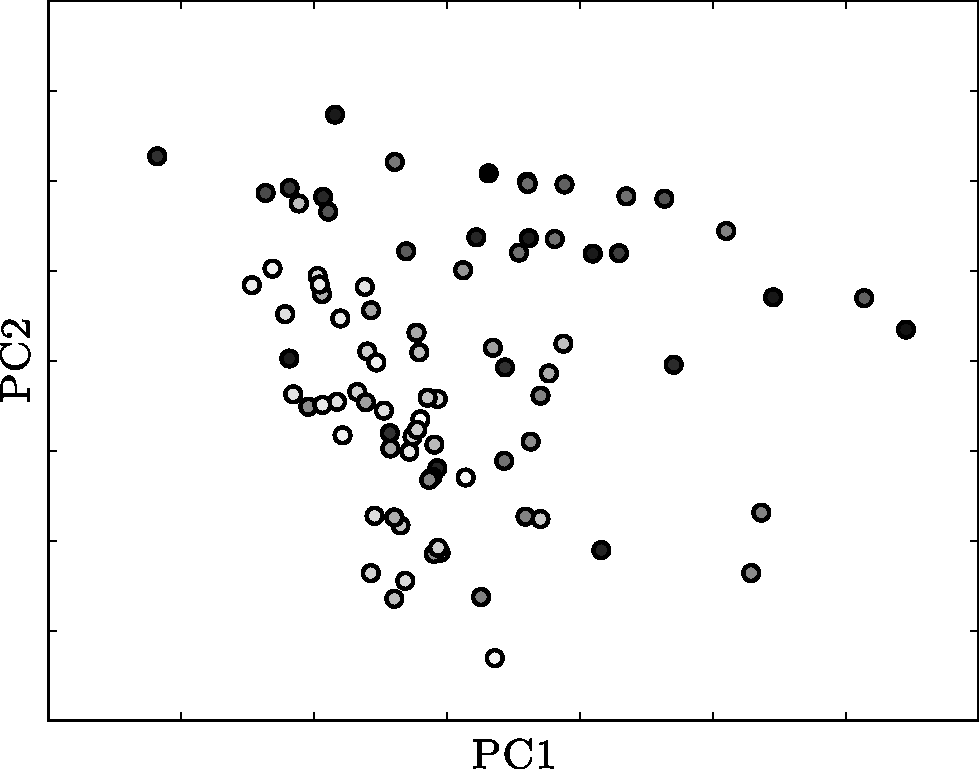
\includegraphics[width=0.5\columnwidth]{img/pca/pca-ace-nofof2}\\
\vspace*{0.8cm}
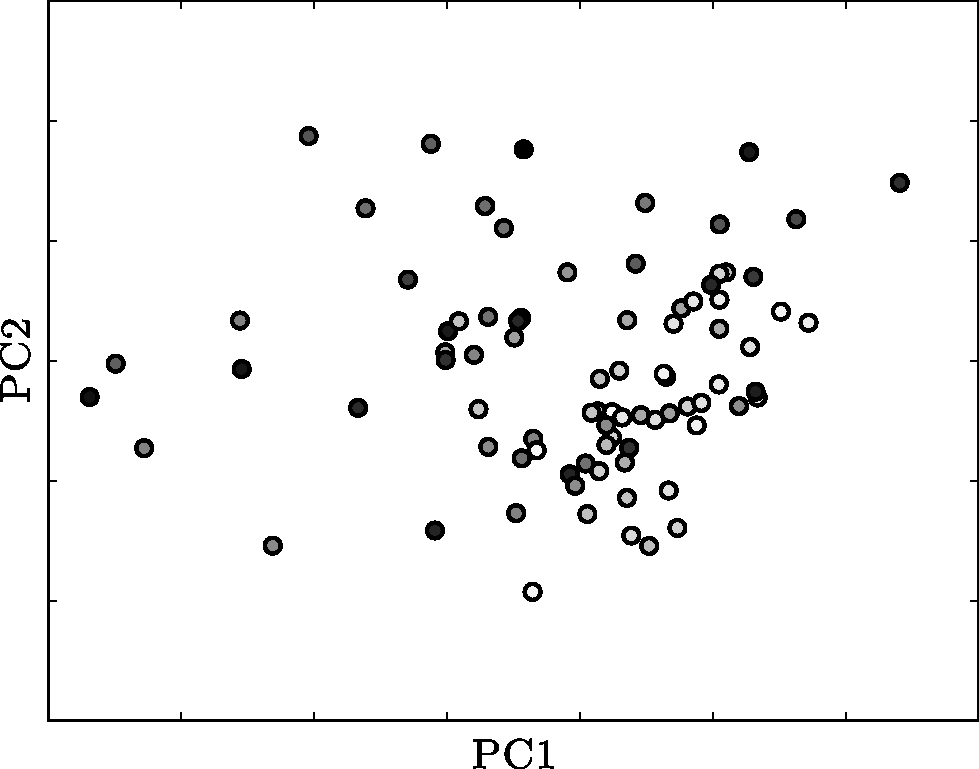
\includegraphics[width=0.5\columnwidth]{img/pca/pca-ace-nofof3}\\
\medskip
\caption[PCA dei reservoir. GraphESN-CF su ACE.]{Plot delle prime due componenti principali dello spazio degli stati dei reservoir nelle sotto-reti. Modello GraphESN-CF applicato al task ACE.\\ 
In scuro gli input con valori target più alti.\\
Reservoir riportati: (\emph{alto}) sotto-rete 1; (\emph{centro}) sotto-rete 5; (\emph{basso}) sotto-rete 9.}
\label{fig:esperimenti:pca-ace-nofof}
\end{figure}

L'efficacia dell'adozione di uno schema di output-feedback è inoltre confermata, secondo un approccio diverso, dall'analisi della capacità di fitting dei modelli. 
La figura~\ref{fig:esperimenti:confronto} mostra il confronto fra l'errore commesso, a parità di iperparametrizzazione ed al crescere della rete. Oltre ai tre proposti è stato in questo caso considerato un quarto modello, consistente in una GraphESN-FOF con connessioni di output-feedback che andassero unicamente verso i reservoir delle sotto-reti successive, e non anche verso il readout. 
Tenendo in considerazione il solo errore commesso sul training-set, ovvero la semplice capacità di fitting dei modelli, risulta evidente dal grafico come l'introduzione di informazione supervisionata attraverso gli output-feedback determini una accresciuta capacità di approssimazione da parte del modello.
\begin{figure}[tbp]
\centering
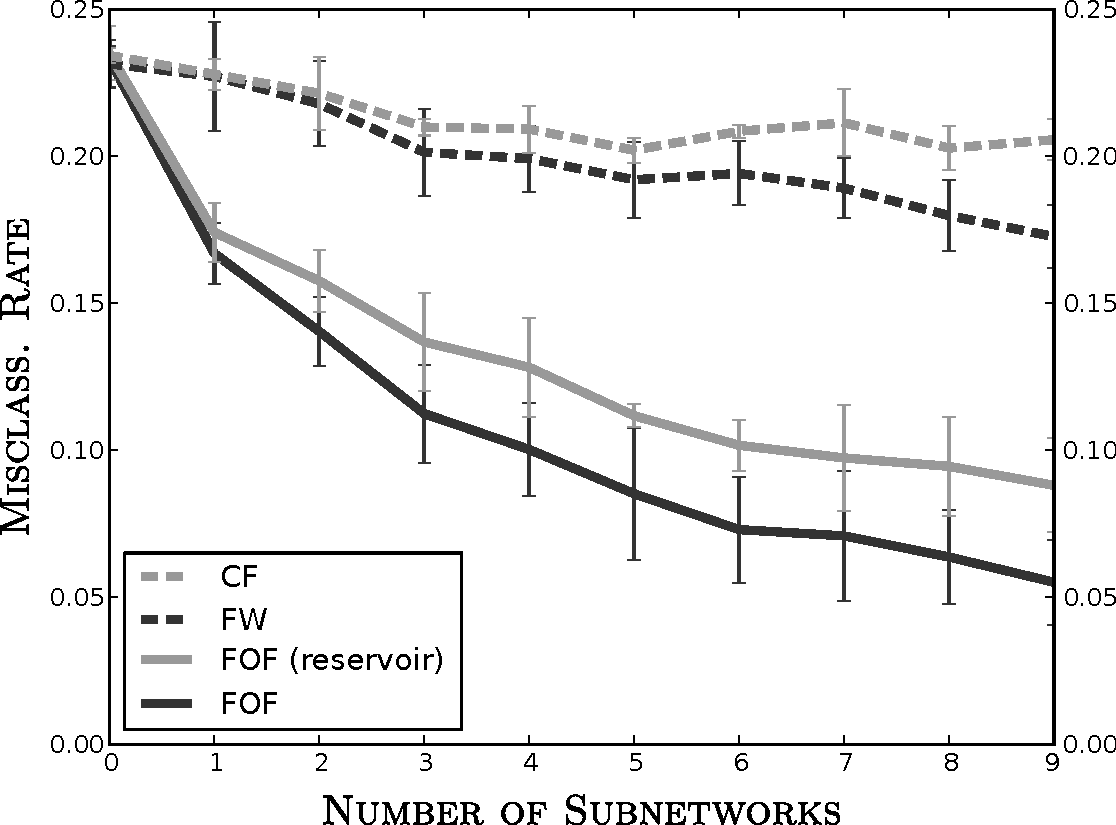
\includegraphics[width=0.7\columnwidth]{img/confronto-modelli-v2}
\medskip
\caption[Confronto fra i modelli: errore di training]{Confronto fra i modelli: errore di training (i.e.\ misclassification rate) e deviazione standard al crescere della rete. Task PTC-FM, $N_R = 100$.}
\label{fig:esperimenti:confronto}
\end{figure}


Dalle analisi supplementari risulta dunque come l'introduzione degli output-feedback rappresenti effettivamente una importante risorsa tesa a potenziare l'encoding delle reti, superando in parte i limiti legati all'uso di reservoir non adattivi. A fronte di questo, le osservazioni sia qualitative che quantitative sui risultati sperimentali suggeriscono l'impiego di forti meccanismi di regolarizzazione e di criteri di stop sofisticati, che impediscano alla rete di accrescere eccessivamente la propria complessità.

Sul piano pratico, gli esperimenti lasciano invece emergere un altro aspetto critico. Poiché per la natura del Reservoir Computing la dimensione del reservoir è estremamente importante ai fini del funzionamento della rete, è infatti necessario stabilire a priori quali siano le dimensioni dei reservoir delle sotto-reti. Nel farlo ci si trova di fronte ad una sorta di trade-off:
\begin{itemize}
\item Con $N_R$ troppo piccolo i reservoir delle sotto-reti perdono la capacità di espandere l'input su uno spazio degli stati ad alta dimensionalità, riducendo la capacità di apprendimento delle sotto-reti e della rete nel suo complesso. In questo scenario, inoltre, si rischia di perdere il vantaggio computazionale, pagando il prezzo di un numero molto alto di iterazioni necessarie alla costruzione della rete (si veda il paragrafo~\vref{sec:modelli:costo}). D'altra parte l'utilizzo di sotto-reservoir di piccole dimensioni offre l'opportunità di avere maggiore controllo sulla crescita della rete, che avverrà in maniera poco discontinua.
\item Con $N_R$ troppo grande si ottengono al contrario singole sotto-reti con una grande capacità di apprendimento che però più facilmente metteranno la rete nella condizione di incappare in situazioni di overfitting. L'aggiunta di una singola sotto-rete determina infatti in questo scenario un aumento elevato, e più difficilmente controllabile, della complessità del modello, rendendo complesso il compito di  apprendere dinamicamente una topologia che sia effettivamente adeguata al task affrontato.
\end{itemize}
Pur consentendo la determinazione automatica della topologia della rete, dunque, l'approccio costruttivo necessita di accorgimenti specifici che permettano di controllare la complessità della rete, attraverso esperienza empirica, criteri di stop sofisticati e l'adozione di meccanismi di regolarizzazione che possano evitare il verificarsi di situazioni di overfitting.












%%%%%%%%%%%%%%%%%%%%%%%%%%%%%%%%%%%%%%%%%%%%%%%%%%%%%%%%%%%%%%%%%%%%%%%%%%%%%%%
%%%%%%%%%%%%%%%%%%%%%%%%%%%%%%%%%%%%%%%%%%%%%%%%%%%%%%%%%%%%%%%%%%%%%%%%%%%%%%%


\begin{comment}

Misclassification-Rate

******************************* PTC FR *****************************************

*** Standard:   TR: 0.309 (stdev. 0.006)    TS: 0.323 (stdev. 0.014)
*** ZERO 50xX:  TR: 0.316 (stdev. 0.009)    TS: 0.327 (stdev. 0.019)
*** ZERO 30xX:  TR: 0.315 (stdev. 0.010)    TS: 0.328 (stdev. 0.018)
*** FW 50xX:    TR: 0.312 (stdev. 0.008)    TS: 0.329 (stdev. 0.010)
*** FW 30xX:    TR: 0.310 (stdev. 0.005)    TS: 0.328 (stdev. 0.004)
*** FOF 50xX:   TR: 0.299 (stdev. 0.007)    TS: 0.317 (stdev. 0.015)
*** FOF 30xX:   TR: 0.299 (stdev. 0.008)    TS: 0.321 (stdev. 0.013)

******************************* PTC FM *****************************************

*** Standard:   TR: 0.351 (stdev. 0.014)    TS: 0.393 (stdev. 0.042)
*** ZERO 50xX:  TR: 0.341 (stdev. 0.017)    TS: 0.372 (stdev. 0.042)
*** ZERO 30xX:  TR: 0.345 (stdev. 0.015)    TS: 0.368 (stdev. 0.044)
*** FW 50xX:    TR: 0.345 (stdev. 0.014)    TS: 0.364 (stdev. 0.044)
*** FW 30xX:    TR: 0.343 (stdev. 0.015)    TS: 0.367 (stdev. 0.038)
*** FOF 50xX:   TR: 0.344 (stdev. 0.017)    TS: 0.375 (stdev. 0.036)
*** FOF 30xX:   TR: 0.347 (stdev. 0.014)    TS: 0.372 (stdev. 0.035)

******************************* PTC MR *****************************************

*** Standard:   TR: 0.400 (stdev. 0.009)	TS: 0.433 (stdev. 0.036)
*** ZERO 50xX:  TR: 0.404 (stdev. 0.009)	TS: 0.421 (stdev. 0.021)
*** ZERO 30xX:  TR: 0.406 (stdev. 0.011)    TS: 0.419 (stdev. 0.019)
*** FW 50xX:    TR: 0.402 (stdev. 0.007)    TS: 0.416 (stdev. 0.017)
*** FW 30xX:    TR: 0.407 (stdev. 0.012)    TS: 0.426 (stdev. 0.021)
*** FOF 50xX:   TR: 0.388 (stdev. 0.017)	TS: 0.428 (stdev. 0.021)
*** FOF 30xX:   TR: 0.389 (stdev. 0.011)	TS: 0.426 (stdev. 0.016)

******************************* PTC MM *****************************************

*** Standard:   TR: 0.326 (stdev. 0.007)    TS: 0.329 (stdev. 0.033)
*** ZERO 50xX:  TR: 0.331 (stdev. 0.004)    TS: 0.350 (stdev. 0.024)
*** ZERO 30xX:  TR: 0.333 (stdev. 0.006)    TS: 0.342 (stdev. 0.023)
*** FW 50xX:    TR: 0.323 (stdev. 0.008)    TS: 0.346 (stdev. 0.032)
*** FW 30xX:    TR: 0.321 (stdev. 0.003)    TS: 0.354 (stdev. 0.027)
*** FOF 50xX:   TR: 0.311 (stdev. 0.012)    TS: 0.334 (stdev. 0.030)
*** FOF 30xX:   TR: 0.319 (stdev. 0.006)	TS: 0.346 (stdev. 0.023)



******************************* Mutag AB ***************************************

*** Standard:   TR: 0.203 (stdev. 0.015)    TS: 0.248 (stdev. 0.130)
*** ZERO 50xX:  TR: 0.150 (stdev. 0.014)	TS: 0.210 (stdev. 0.103) 
*** ZERO 30xX:  TR: 0.159 (stdev. 0.010)    TS: 0.204 (stdev. 0.102) 
*** FW 50xX:    TR: 0.138 (stdev. 0.009)    TS: 0.195 (stdev. 0.099)
*** FW 30xX:    TR: 0.141 (stdev. 0.009)    TS: 0.203 (stdev. 0.106)
*** FOF 50xX:   TR: 0.126 (stdev. 0.014)    TS: 0.207 (stdev. 0.053)
*** FOF 30xX:   TR: 0.131 (stdev. 0.007)    TS: 0.232 (stdev. 0.079)


******************************* Mutag AB+C *************************************

*** Standard:   TR: 0.163 (stdev. 0.019)    TS: 0.235 (stdev. 0.094)
*** ZERO 50xX:  TR: 0.162 (stdev. 0.022)    TS: 0.219 (stdev. 0.085)
*** ZERO 30xX:  TR: 0.174 (stdev. 0.025)    TS: 0.240 (stdev. 0.083)
*** FW 50xX:    TR: 0.163 (stdev. 0.016)    TS: 0.237 (stdev. 0.084)
*** FW 30xX:    TR: 0.161 (stdev. 0.018)    TS: 0.233 (stdev. 0.083)
*** FOF 50xX:   TR: 0.149 (stdev. 0.022)    TS: 0.240 (stdev. 0.075)
*** FOF 30xX:   TR: 0.159 (stdev. 0.027)    TS: 0.230 (stdev. 0.060)


******************************* Mutag AB+C+PS **********************************

*** Standard:   TR: 0.162 (stdev. 0.022)    TS: 0.197 (stdev. 0.066)
*** ZERO 50xX:  TR: 0.161 (stdev. 0.020)    TS: 0.206 (stdev. 0.085)
*** ZERO 30xX:  TR: 0.164 (stdev. 0.020)    TS: 0.203 (stdev. 0.082)
*** FW 50xX:    TR: 0.157 (stdev. 0.024)    TS: 0.207 (stdev. 0.083)
*** FW 30xX:    TR: 0.166 (stdev. 0.023)    TS: 0.194 (stdev. 0.072)
*** FOF 50xX:   TR: 0.158 (stdev. 0.021)    TS: 0.201 (stdev. 0.073)
*** FOF 30xX:   TR: 0.157 (stdev. 0.023)	TS: 0.200 (stdev. 0.080)

\end{comment}
 \chapter{Conclusioni}\label{ch:conclusioni}
%Riassumere (fra una pagina) i tipi di modelli introdotti a complessità crescente con flat, cascade in output, poi cascade anche nel reservoir
Nel corso della tesi sono stati presentati dei nuovi modelli di Reti Neurali Ricorsive per l'apprendimento supervisionato di trasduzioni strutturali su grafi. 
I modelli proposti estendono le GraphESN attraverso un approccio costruttivo, innovativo nell'ambito del Reservoir Computing, che consente di costruire la rete progressivamente. Ereditando dalle GraphESN la capacità di apprendere trasduzioni strutturali generiche attraverso algoritmi di apprendimento efficienti, i modelli presentati sfruttano la strategia costruttiva per offrire soluzioni originali ad alcuni dei problemi aperti nell'ambito del Reservoir Computing. 

% topologia automatica
L'approccio costruttivo consente nei modelli proposti di determinare in maniera automatica (i.e.\ guidata dal task affrontato) il numero di unità che compongono la rete nel suo complesso e la sua topologia. Questa caratteristica permette di non dover fissare a priori la dimensione e la struttura della rete, in contrapposizione con quanto avviene per i modelli di Reservoir Computing esistenti, che fanno affidamento su reservoir prefissati. Tale vantaggio acquista rilievo se si considera che la dimensione del reservoir risulta essere un fattore estremamente importante per caratterizzare la complessità della rete. 
La determinazione automatica del numero di unità ha quindi anche l'effetto di ridurre il costo computazionale necessario alla selezione del modello.

% output-feedback
Sfruttando la strategia costruttiva è stato inoltre realizzato un meccanismo stabile di output-feedback, usato per modificare le dinamiche dei reservoir. Nel corso del procedimento incrementale di costruzione della rete, infatti, i modelli costruttivi possono avvalersi delle informazioni già apprese in precedenza che, attraverso uno schema di connessioni fra le sotto-reti, sono state introdotte all'interno del processo di codifica dell'input.
Anche in presenza di reservoir prefissati e non soggetti ad alcun tipo di adattamento, dunque, i modelli proposti risultano in grado di sfruttare, durante il procedimento di encoding, delle informazioni supervisionate, direttamente dipendenti dal task.
Lo schema di output-feedback individua quindi una possibile strategia per affrontare uno dei problemi aperti caratteristici del Reservoir Computing: la presenza di reservoir fissati a priori e non adattivi, con dinamiche interne unicamente guidate dalla natura degli input e non legate anche al problema affrontato.

% descrizione modelli
Le soluzioni proposte sono state sviluppate secondo un processo incrementale, da cui sono derivati tre distinti modelli, ognuno in grado di generalizzare i precedenti. La strategia costruttiva è stata introdotta attraverso il modello GraphESN-CF, in grado di determinare automaticamente le dimensioni di una rete con topologia flat (i.e.\ con un unico livello di sotto-reti). Il modello GraphESN-FW ha esteso il precedente introducendo delle connessioni fra le sotto-reti, in modo da realizzare una rete di tipo Reservoir Computing con topologia multilayer non lineare. Con il modello GraphESN-FOF si è infine ulteriormente estesa la struttura delle connessioni fra le sotto-reti, sfruttando gli output-feedback per guidare il processo di encoding coerentemente con il task trattato.

% efficienza douta alla scomposizione del problema
I modelli realizzati si caratterizzano per una notevole flessibilità ed efficienza dal punto di vista computazionale. 
L'opportunità di suddividere un task in sotto-problemi consente di ampliare la gamma di strategie utilizzabili nell'allenamento e permette di ricorrere a strumenti caratteristici dell'approccio costruttivo, come l'impiego di un pool. Oltre a questo, la decomposizione del problema offre la possibilità di impiegare sotto-reti di dimensioni contenute, specializzate a risolvere solo un sotto-task specifico, determinando così un notevole vantaggio computazionale nella realizzazione dell'allenamento della rete nel suo complesso. Anche guardando al solo ambito del Reservoir Computing, di per sé caratterizzato da oneri computazionali estremamente ridotti, i modelli realizzati permettono quindi di guadagnare in efficienza senza che questo comporti perdite in accuratezza di predizione.

% esperimenti
L'efficacia dei modelli realizzati è stata testata su problemi reali appartenenti all'ambito della Chemioinformatica. 
Gli esperimenti svolti hanno mostrato nei modelli proposti la capacità di ottenere un'accuratezza nelle predizioni comparabile, ed in molti casi migliore, rispetto ai modelli non costruttivi.
%Gli esperimenti svolti hanno mostrato come i modelli proposti, nonostante richiedano un impiego inferiore di risorse computazionali, siano in grado in molti casi di migliorare le performance raggiunte attraverso l'utilizzo di modelli non costruttivi. 
Il ruolo degli output-feedback è stato indagato attraverso un approccio sia quantitativo che qualitativo, mettendo in luce come l'introduzione di informazione supervisionata all'interno dei reservoir sia effettivamente in grado di influenzarne le dinamiche in maniera coerente con il task affrontato, in netta contrapposizione con quanto avviene in assenza di output-feedback. 
% criticità
L'analisi sperimentale ha anche fatto emergere alcuni aspetti critici nei modelli proposti. L'impiego di output-feedback verso i reservoir non risulta infatti in maniera sistematica in un aumento della capacità di generalizzazione dei modelli, suggerendo quindi l'adozione di meccanismi di regolarizzazione forti, tesi ad evitare situazioni di overfitting. Inoltre, benché le dimensioni della rete siano determinate in maniera automatica, il numero di unità che compongono i reservoir delle sotto-reti risulta essere un fattore importante per le capacità dei modelli. La determinazione di un valore adeguato per tale parametro può tuttavia essere affrontata tramite un processo di selezione che coinvolga l'esperienza empirica o, eventualmente, attraverso il processo di model selection.

% spunti futuri (estendere)
L'aver indirizzato un approccio innovativo nel campo del Reservoir Computing fornisce anche spunti per ulteriori sperimentazioni. 
La strategia costruttiva proposta è estremamente flessibile ed è ragionevole ipotizzare che altre varianti topologiche, oltre a quelle realizzate, possano essere oggetto di investigazione. I modelli sperimentati sfruttano infatti uno schema di connessioni fra le sotto-reti molto semplice, che può facilmente essere modificato in modo da implementare, ad esempio, politiche di propagazione degli output-feedback che tengano conto della topologia (e.g.\ collegando una sotto-rete solo alle sotto-reti più prossime) o delle performance (e.g.\ assegnando alle connessioni pesi differenti in base alle performance ottenute dalle singole sotto-reti).
Altrettanto importante e variegata è anche la gamma degli algoritmi di learning o dei sotto-task utilizzabili per l'allenamento delle sotto-reti, anch'essa possibile oggetto di ulteriori indagini così come l'impiego di sotto-reti eterogenee (e.g.\ nella dimensione del reservoir) selezionate tramite un pool.

\`E infine opportuno sottolineare che parte dei contenuti discussi nel corso della tesi sono stati riportati nell'articolo \textit{Constructive Reservoir Computation with Output Feedbacks for Structured Domains} \cite{Gallicchio:ConstructiveReservoir}, che verrà discusso nel corso del XX European Symposium on Artificial Neural Networks, Computational Intelligence and Machine Learning.






%\begin{comment}
%
%Limitando gli effetti dell'utilizzo di reservoir prefissati e non adattivi, l'approccio costruttivo consente infatti di determinare in maniera automatica il numero di unità e la topologia della rete ed offre la possibilità di realizzare uno schema stabile di output-feedback, in grado di introdurre informazione supervisionata nel processo di encoding dei reservoir.
%
%I modelli proposti si caratterizzano per l'introduzione di un approccio costruttivo nell'ambito del Reservoir Computing, sfruttato per offrire soluzioni ad alcuni dei problemi aperti in questo campo. L'adozione di una strategia costruttiva permette infatti di determinare in maniera automatica il numero di unità e la topologia della rete e consente l'introduzione di uno schema di output-feedback stabile, in grado di introdurre informazione supervisionata nel processo di encoding dei reservoir.
%
%
%
%L'aver adottato una strategia costruttiva ha permesso la formulazione di modelli molto efficienti dal punto di vista computazionale. L'allenamento ed il processo di model selection per le reti proposte risultano infatti vantaggiosi anche se si guarda al solo ambito del Reservoir Computing, di per sé caratterizzato da oneri computazionali estremamente ridotti. In quest'ottica, quanto realizzato si configura come uno strumento pratico ed efficace nel trattamento di domini strutturati che permette di guadagnare in efficienza senza comportare perdite in termini di accuratezza di predizione.
%
%Con l'introduzione di un sistema stabile di output-feedback si è invece implementato un meccanismo che permetta di sfruttare la presenza di informazione supervisionata all'interno del processo di encoding del Reservoir Computing. L'uso di informazioni di questo tipo è stato possibile grazie alla fusione di due mondi ad oggi separati, quello del Reservoir Computing e quello delle Reti Neurali Costruttive, e dà risposta, anche se in maniera parziale, ad un'esigenza già emersa nella sfera del Reservoir Computing.
%
%L'efficacia dei modelli realizzati è stata testata su problemi reali appartenenti all'ambito della Chemioinfomatica. Gli esperimenti svolti hanno mostrato come i modelli proposti, nonostante richiedano un impiego inferiore di risorse computazionali, siano in grado in molti casi di migliorare le performance raggiunte attraverso l'utilizzo di modelli non costruttivi. L'analisi sperimentale ha inoltre messo in luce gli effetti degli output-feedback sugli stati dei reservoir, evidenziando come il loro impiego possa effettivamente arricchirne le dinamiche, influenzandole in maniera consistente con il task affrontato.
%
%Il lavoro svolto ha anche messo in luce alcune criticità. Il ruolo positivo degli output-feedback, ad esempio, non è completamente supportato dai risultati sperimentali, almeno in termini di performance. Non sempre, infatti, il loro impiego ha comportato un miglioramento della capacità di generalizzazione della rete. Oltre a questo, il numero di unità nel reservoir rimane comunque un iperparametro critico, limitando i benefici derivanti dall'approccio costruttivo. Entrambi questi aspetti possono essere oggetto di ulteriori ricerche.
%
%L'aver indirizzato un approccio innovativo nel campo del Reservoir Computing lascia inoltre emergere ulteriori spunti di sperimentazione. La strategia costruttiva proposta è infatti estremamente flessibile ed è ragionevole ipotizzare che molte altre varianti topologiche, oltre a quelle proposte, possano essere oggetto di investigazione. Altrettanto importante e variegata è anche la gamma degli algoritmi di learning o dei sotto-task utilizzabili per l'allenamento delle sotto-reti, anch'essa possibile oggetto di ulteriori indagini così come l'impiego di sotto-reti eterogenee selezionate tramite un pool.
%
%\`E infine opportuno sottolineare come parte dei contenuti della tesi siano oggetto dell'articolo \textit{Constructive Reservoir Computation with Output Feedbacks for Structured Domains} \cite{Gallicchio:ConstructiveReservoir}, che sarà presentato nel corso del XX European Symposium on Artificial Neural Networks, Computational Intelligence and Machine Learning.
%
%
%
%Parte dei risultati riportati nel seguito è inoltre discussa nell'articolo scientifico \textit{Constructive Reservoir Computation with Output Feedbacks for Structured Domains}, inviato all'European Symposium on Artificial Neural Networks, Computational Intelligence and Machine Learning\footnote{\url{http://www.dice.ucl.ac.be/esann/}} ed attualmente in fase di revisione.
%
%Pro:
%\begin{itemize}
%\item Approccio costruttivo ed output-feedback stabili (vedi draft)
%\item Dire del draft / Siamo alla frontiera della ricerca 
%\item Ci siamo misurati con problemi del mondo reale
%\item Efficienza computazionale (importante)
%\item Trattamento di grafi ciclici/indiretti.
%\item Fase di codifica non adattiva ma neppure manuale
%\item L'approccio costruttivo nelle ESN di fatto non esiste, anche se Luko lo lascia intendere.
%\end{itemize}
%
%Contro / future works:
%\begin{itemize}
%\item I vantaggi computazionali non sono esattamente quelli di una cascade correlation, visto che le GraphESN già usano algoritmi di training efficienti (in CC evitavamo la BackPropagation).
%\item Gli output-feedback non ``staccano'' nettamente gli altri modelli, eppure diverse cose ci dicono che possono funzionare.
%\item Le strategie possibili sono molte di più di quelle effettivamente sperimentate: topologia, training, sotto-task, criteri di stop.
%\item Evitare l'allenamento del readout, come nell'articolo trovato da Claudio (che però non trovo in pdf).
%\item Il numero di unità del reservoir.
%\end{itemize}
%
%% In una cascade correlation tutti i pesi vengono allenati e l'approccio costruttivo permette di ``spezzettare'' questo lavoro in più parti, meno onerose (n.b. non usa backpropagation!). Noi non siamo esattamente in questa situazione, o almeno non del tutto: nel nostro caso l'allenamento è semplice di suo.
%
%% Costo computazionale mica pizza e fichi
%
%% Luko quando parla dei feedback e lascia intendere l'approccio costruttivo
%
%% L'articolo che ha trovato Claudio suggerisce la possibilità di non allenare affatto il readout-globale.
%
%% Molte possibili strategie, molte più di quelle sperimentate/riportate: nella topologia, nel training, nei sotto-task.
%
%\end{comment} 

\appendix
 \chapter{Dettaglio del costo computazionale}\label{app:costo}
\newcommand{\NSN}{\mathit{NSN}}
\newcommand{\MAXV}{\mathit{MAXV}}
\newcommand{\MAXIT}{\mathit{MAXIT}}
\newcommand{\Nr}{\ensuremath{N_R}}
\newcommand{\Ny}{\ensuremath{N_Y}}
\newcommand{\Nz}{\ensuremath{N_Z}}
\newcommand{\Nu}{\ensuremath{N_U}}
\newcommand{\Nf}{\ensuremath{N_F}}
\newcommand{\G}{\ensuremath{\abs{\mathcal{G}}}}
Consideriamo una rete di tipo GraphESN-FOF formata da $\NSN$ sotto-reti con reservoir completamente connessi di dimensione $\Nr$.
Indichiamo con $\Nz$ la dimensione dell'output delle sotto-reti e con $\Ny$ quella del readout globale, entrambe trascurabili visto che tipicamente $\Ny = \Nz = 1$. Sia $\Nu$ la dimensione delle etichette associate ad ogni vertice dell'input e $\G$ la dimensione del dataset (i.e il numero totale di input). 

Di seguito, nei paragrafi~\ref{app:costo:encoding}-\ref{app:costo:out_globale} viene riportato il calcolo del costo computazionale relativo alle varie fasi di utilizzo del modello: encoding dei dati, allenamento delle sotto-reti, allenamento del readout-globale, calcolo dell'output.

Il paragrafo~\ref{app:costo:modelselection} riporta invece il calcolo del costo computazionale per la model selection di una GraphESN standard.


%%%%%%%%%%%%%%%%%%%%
\section{Encoding dei dati}\label{app:costo:encoding}
Consideriamo un singolo passo del processo di encoding nella rete $i$-esima. 
\begin{equation}
	\vect{x}^{(i)}_t(v) = f( 
	\matr{W}^{(i)}_\textup{in} \, \vect{u}(v) + 
	\sum_{w \in \mathcal{N}(v)} \hat{\matr{W}}^{(i)} \, \vect{x}^{(i)}_{t-1}(w) +
	\sum_{j=1}^{i-1} \matr{W}^{(ij)}_\textup{fof} \, \vect{z}^{(j)}(v)
	)
\end{equation}
con $\matr{W}^{(i)}_\textup{in} \in \R^{\Nr \times \Nu}$, $\hat{\matr{W}}^{(i)} \in \R^{\Nr \times \Nr}$, $\matr{W}^{(ij)}_\textup{fof} \in \R^{\Nr \times \Nz}$.

Indicando con $\MAXV$ il numero massimo di vertici di un grafo di input, il costo per l'encoding di un grafo $\graph{g}$ è dato dalla somma dei costi:
\begin{itemize}
\item $\matr{W}^{(i)}_\textup{in} \, \vect{u}(v)$, ha costo $O(\Nr\ \Nu)$ e viene calcolato una sola volta per ogni vertice del'input.
\item $\sum_{j=1}^{i-1} \matr{W}^{(ij)}_\textup{fof} \, \vect{z}^{(j)}(v)$, ha costo $O(\Nr\ \Ny\ (i-1))$ e viene calcolato una sola volta per ogni vertice dell'input.
\item $\sum_{w \in \mathcal{N}(v)} \hat{\matr{W}}^{(i)} \, \vect{x}^{(i)}_{t-1}(w)$, ha costo $O(\Nr^2)$ e viene calcolato per ogni vertice ad ogni iterazione.
\end{itemize}
Chiamando $\MAXIT$ il numero massimo di iterazioni, il costo dell'encoding di un singolo grafo è dunque  dato da
\begin{equation}
O(\Nr\ \Nu\ \MAXV + \Nr\ \Ny\ (i-1)\ \MAXV + \Nr^2\ \MAXV\ \MAXIT))
\end{equation}
che, ripetuto per $\G$ volte, ovvero per ogni grafo nel dataset, è
\begin{equation}
\begin{array}{l}
O(\G\ (\Nr\ \Nu\ \MAXV + \Nr\ \Ny\ (i-1)\ \MAXV + \Nr^2\ \MAXV\ \MAXIT)) \\
\simeq O(\G\ \Nr^2\ \MAXV\ \MAXIT)
\end{array}
\end{equation}
che scala quadraticamente con la dimensione del reservoir, rendendo trascurabile la presenza delle connessioni di output-feedback.

Per l'intera rete, ovvero considerando tutte le $\NSN$ sottoreti, il costo complessivo del processo di encoding è dato da
\begin{equation}
O(\NSN\ \G\ \Nr^2\ \MAXV\ \MAXIT)
\end{equation}
e scala linearmente con la dimensione del dataset e dei grafi e quadraticamente con la dimensione del reservoir.

Considerando l'uso di reservoir sparsi, con al più $M$ connessioni in ingresso ad ogni unità, il costo computazionale dell'encoding può essere ulteriormente ridotto a 
\begin{equation}
O(\NSN\ \G\ \Nr\ M\ \MAXV\ \MAXIT)
\end{equation}
che dipende linearmente dalla dimensione del reservoir e da $M$.

%%%%%%%%%%%%%%%%%
\section{Training delle sotto-reti}\label{app:costo:tr_sub}
Consideriamo il caso in cui la rete i-esima sia allenata tramite Ridge Regression. In formula:
\begin{equation}\label{app:costo:ridgeregr}
\transpose{\matr{W}_\textup{out}} = (\matr{X}^T \matr{X} + \lambda_\textup{r} \matr{I})^{-1} \matr{X}^T \matr{Y}_\textup{target}
\end{equation}
con $\matr{X} \in \R^{\G \times (\Nr + \Nz (i-1))}$ matrice che contiene tutti gli input del readout (i.e. per ogni grafo, la codifica ottenuta dal sotto-reservoir più gli output-feedback provenienti dalle sotto-reti precedenti), $\matr{Y}_\textup{target} \in \R^{\G \times \Ny}$ contenente i valori target (i.e. un vettore di uscita per ogni input) e $\matr{I} \in \R^{(\Nr + \Nz (i-1)) \times (\Nr + \Nz (i-1))}$ matrice identità.

Chiamiamo per semplicità $\Nf(i) = \Nr + \Nz\, (i-1)$, ad indicare il numero di \emph{features} in input al readout $i$-esimo.
I singoli passaggi nel calcolo della Ridge Regression hanno il seguente costo:
\begin{itemize}
\item $\matr{X}^T \matr{X}$, prodotto di matrici: $O(\Nf(i)^2\ \G)$.
\item $(\matr{X}^T \matr{X} + \lambda_\textup{r} \matr{I})^{-1}$, inversione: $O(\Nf(i)^3)$.
\item $\matr{X}^T \matr{Y}_\textup{target}$, prodotto di matrici: $O(\Nf(i)\ \G\ \Nz)$.
\item $(\matr{X}^T \matr{X} + \lambda_\textup{r} \matr{I})^{-1} \matr{X}^T \matr{Y}_\textup{target}$, prodotto di matrici: $O(\Nf(i)^2 \Nz)$.
\end{itemize}
Il costo complessivo per l'allenamento della sotto-rete $i$-esima è quindi dato da:
\begin{equation}
\begin{array}{l}
O(\Nf(i)^3 + \Nf(i)^2\ \G + \Nf(i)^2 \Nz + \Nf(i)\ \G\ \Nz) \\
\simeq O(\Nf(i)^3 + \Nf(i)^2\ \G + \Nf(i)^2 + \Nf(i)\ \G\ ) \\
\simeq O(\Nf(i)^3 + \Nf(i)^2\ \G ) \\
\end{array}
\end{equation}

Nel passaggio da una singola sotto-rete alla rete nel suo complesso bisogna tener conto del fatto che $\Nf$ è funzione di $i$ (i.e.$\Nf(i) = \Nr + \Nz\, (i-1)$).
Il costo dell'allenamento di $\NSN$ sotto-reti è quindi dato da
\begin{equation}\label{app:costo:ridge}
\begin{array}{l}
O(\sum_{i=1}^{\NSN} (\Nf(i)^3 + \Nf(i)^2\ \G)) \\
= O(\sum_{i=1}^{\NSN} \Nf(i)^3 + \sum_{i=1}^{\NSN} \Nf(i)^2\ \G) \\
\end{array}
\end{equation}
Per semplicità, consideriamo le due sommatorie separatamente.
\begin{equation}\label{app:costo:ridge1}
\begin{array}{l}
\displaystyle O(\sum_{i=1}^{\NSN} \Nf(i)^3) = O(\sum_{i=1}^{\NSN} (\Nr + \Nz (i-1))^3) \\
\displaystyle = O(\sum_{i=1}^{\NSN} (\Nr^3 + 3 \Nr^2\ \Nz\ (i-1) + \Nz^3\ (i-1)^3 + 3 \Nr\ \Nz^2\ (i-1)^2)\\
\displaystyle = O(\NSN\ \Nr^3 + 3 \Nr^2\ \Nz \sum_{i=1}^{\NSN} (i-1) + \Nz^3 \sum_{i=1}^{\NSN} (i-1)^3 + 3 \Nr\ \Nz^2 \sum_{i=1}^{\NSN} (i-1)^2 )\\
\displaystyle \simeq O(\NSN\ \Nr^3 + \Nr^2\ \sum_{i=1}^{\NSN} (i-1) + \sum_{i=1}^{\NSN} (i-1)^3 + \Nr\ \sum_{i=1}^{\NSN} (i-1)^2 )\\
\displaystyle \simeq O(\NSN\ \Nr^3 + \Nr^2\ \NSN^2 + \NSN^4 + \Nr\ \NSN^3 )\\
\end{array}
\end{equation}
la seconda parte dell'equazione (\ref{app:costo:ridge}) è invece data da
\begin{equation}\label{app:costo:ridge2}
\begin{array}{l}
\displaystyle O(\sum_{i=1}^{\NSN} \Nf(i)^2\ \G)\\
\displaystyle = O(\G  \sum_{i=1}^{\NSN} (\Nr + \Nz\ (i-1))^2) \\
\displaystyle = O(\G  \sum_{i=1}^{\NSN} (\Nr^2 + 2 \Nr\ \Nz\ (i-1) + \Nz^2 (i-1)^2)) \\
\displaystyle = O(\G  (\NSN\ \Nr^2 + 2\Nr\ \Nz \sum_{i=1}^{\NSN}(i-1) + \Nz^2 \sum_{i=1}^{\NSN}(i-1)^2)\\
\displaystyle \simeq O(\G (\NSN\ \Nr^2 + \Nr\ \NSN^2 + \NSN^3)) \\
\displaystyle = O(\NSN\ \Nr^2\ \G + \Nr\ \NSN^2\ \G + \NSN^3\ \G) \\
\end{array}
\end{equation}

Mettendo insieme le equazioni (\ref{app:costo:ridge1}) e (\ref{app:costo:ridge2}) si ottiene il costo complessivo dell'allenamento delle sotto-reti tramite Ridge Regression:
\begin{multline}
O(\NSN^4 + \Nr\ \NSN^3 + \Nr^2\ \NSN^2 + \NSN\ \Nr^3 \\
+ \NSN^3\ \G + \NSN^2\ \Nr\ \G + \NSN\ \Nr^2\ \G)
\end{multline}

%%%%%%%%%%%%%%%%%%%%%%%%%
\section{Training del readout globale}
Consideriamo due possibili casi di allenamento per il readout globale: l'applicazione dell'algoritmo diretto di Ridge Regression o l'impiego dell'algoritmo iterativo LMS.


\subsection{Ridge Regression}\label{app:costo:tr_globale_ridge}
Nel caso in cui il readout globale sia allenato tramite Ridge Regresison, la formula ricalca quella riportata nell'equazione (\ref{app:costo:ridgeregr}), in cui però la dimensione degli input è data solo dagli output delle sotto-reti (i.e. senza alcun input proveniente da un reservoir), quindi $\matr{X} \in \R^{\G \times \Nz\, (i-1)}$.\\
Chiamando $\Nf(i) = \Nz\, (i-1)$, il costo computazionale per l'allenamento della rete al passo $i$-esimo è dato da
\begin{equation}
O(\Nf(i)^3 + \Nf(i)^2\ \G)
\end{equation}
Il costo complessivo dell'allenamento del readout globale è quindi:
\begin{equation}
\begin{array}{l}
\displaystyle O(\Nf(i)^3 + \Nf(i)^2\ \G) \\
\displaystyle = O(\sum_{i=1}^{\NSN} (\Nz^3\ (i-1)^3 + (\Nz^2\ (i-1)^2\ \G) \\
\displaystyle = O(\Nz^3\ \sum_{i=1}^{\NSN}(i-1)^3 + \Nz^2\ \G\ \sum_{i=1}^{\NSN}(i-1)^2) \\
\displaystyle \simeq O(\NSN^4 + \NSN^3 \G)\\
\end{array}
\end{equation}

\subsection{LMS}\label{app:costo:tr_globale_lms}
In questo caso l'algoritmo è iterativo. Chiamiamo $\MAXIT$ il numero massimo di iterazioni necessarie perché l'algoritmo converga.
L'allenamento del readout globale, dopo aver aggiunto $i$ sotto-reti, è dato da
\begin{equation}
O(\MAXIT\ \G\ (i-1)\ \Ny^2)
\end{equation}

Complessivamente, il costo necessario all'allenamento del readout globale della rete tramite LMS è quindi
\begin{equation}
\begin{array}{l}
\displaystyle O(\sum_{i=1}^{\NSN} (\MAXIT\ \G\ (i-1)\ \Ny^2)) \\
\displaystyle = O(\MAXIT\ \Ny^2\ \G\ \sum_{i=1}^{\NSN} (i-1)) \\
\displaystyle \simeq O(\MAXIT\ \Ny^2\ \G\ \NSN^2) \\
\displaystyle \simeq O(\MAXIT\ \G\ \NSN^2) \\
\end{array}
\end{equation}


%%%%%%%%%
\section{Calcolo dell'output delle sotto-reti}\label{app:costo:out_sub}
Per il calcolo dell'output tutti i valori di input --- sia provenienti dal reservoir che gli output-feedback --- sono calcolati in precedenza. Il calcolo dell'uscita della rete $i$-esima per il grafo $\graph{g}$ corrisponde dunque alla moltiplicazione
\begin{equation}\label{app:eq:ro:sub}
\matr{W}^{(i)}_\textup{out} \,
		[\mathcal{X}(\vect{x}^{(i)}(\graph{g})), \vect{z}^{(1)}(\graph{g}), \dots, \vect{z}^{(i-1)}(\graph{g})]
\equiv \matr{W}^{(i)}_\textup{out} \, \vect{v}_\textup{feat} 
\end{equation}
con $\matr{W}^{(i)}_\textup{out} \in \R^{\Nz \times (\Nr + \Nz\, (i-1))}$ ed il vettore  $\vect{v}_\textup{f} \in \R^{\Nr + \Nz\, (i-1)}$ ad indicare la concatenazione delle features in input al readout (i.e. encoding del reservoir più output-feedback).

Il costo per il calcolo dell'uscita della sotto-rete $i$-esima per tutti i grafi del dataset è dunque
\begin{equation}
\begin{array}{l}
O(\G\ \Nz (\Nr + \Nz\, (i-1)) \\
= O(\G\ \Nz\ \Nr + \G\ \Nz^2, (i-1)) \\
\end{array}
\end{equation}
Considerando tutte le $\NSN$ sotto-reti, si ottiene il costo complessivo:
\begin{equation}
\begin{array}{l}
\displaystyle O(\sum_{i=1}^{\NSN} (\G\ \Nz\ \Nr + \G\ \Nz^2, (i-1))) \\
\displaystyle = O(\NSN\ \G\ \Nz \Nr + \G\ \Nz^2 \sum_{i=1}^{\NSN} (i-1))\\
\displaystyle \simeq O(\NSN\ \G\ \Nr + \G\ \NSN^2)
\end{array}
\end{equation}

%%%%%%%%%
\section{Calcolo dell'output del readout globale}\label{app:costo:out_globale}
Questo caso differisce dal calcolo dell'output delle sotto-reti unicamente perché l'input del readout globale è formato dai soli output-feedback, senza che vi sia alcun segnale proveniente da un reservoir. \\
Il costo computazionale complessivo per il calcolo degli output della rete è quindi dato da
\begin{equation}
O(\G\ \NSN^2)
\end{equation}
e scala linearmente con la dimensione del dataset e quadraticamente con il numero di sotto-reti.


%%%%%%%%%%
\section{Model selection di GraphESN}\label{app:costo:modelselection}
Assumiamo l'uso di una GraphESN con reservoir completamente connessi. Siamo interessati al costo complessivo di una model selection che preveda la variazione delle dimensioni del reservoir: $\Nr' \in \lbrace \Nr, 2\Nr, \dots, \NSN\, \Nr \rbrace$.

Il costo del processo di encoding di una singola rete con reservoir di dimensioni $\Nr$ è in questo caso
\begin{equation}
O(\Nr^2\ \MAXIT\ \MAXV\ \G)
\end{equation}
Facendo variare la dimensione del reservoir, il costo complessivo diventa
\begin{equation}
\begin{array}{l}
\displaystyle O(\Nr^2\ \MAXIT\ \MAXV\ \G \sum_{i=1}^{\NSN} i^2) \\
\displaystyle \simeq O(\Nr^2\ \MAXIT\ \MAXV\ \G \NSN^3)
\end{array}
\end{equation}

L'apprendimento, tramite Ridge Regression, ha invece per una singola rete costo complessivo di
\begin{equation}
O(\Nr^3 + \Nr^2\ \G)
\end{equation}
variando $\Nr' \in \lbrace \Nr, 2\Nr, \dots, \NSN\, \Nr \rbrace$ si ha dunque
\begin{equation}
\begin{array}{l}
\displaystyle O(\Nr^3\ \sum_{i=1}^{\NSN} i^3 + \Nr^2\ \G\ \sum_{i=1}^{\NSN} i^2) \\
\displaystyle \simeq O(\Nr^3\ \NSN^4 + \Nr^2\ \G\ \NSN^3) \\
\end{array}
\end{equation}

Infine, il calcolo dell'output per ogni input del dataset costa
\begin{equation}
O(\Nr\ \G)
\end{equation}
che nel caso di una model selection completa diventa
\begin{equation}
\displaystyle O(\Nr\ \G \sum_{i=1}^{\NSN} i) \\
\displaystyle \simeq O(\Nr\ \G \NSN^2) \\
\end{equation}

Il costo complessivo della selezione di un modello di tipo GraphESN, ottenuto variando la dimensione del reservoir $\Nr' \in \lbrace \Nr, 2\Nr, \dots, \NSN\, \Nr \rbrace$ è dunque:
\begin{multline}
O(\NSN^4\ \Nr^3 + \NSN^3\ \Nr^2\ \MAXIT\ \MAXV\ \G \\
+ \NSN^3\ \Nr^2\ \G + \NSN^2\ \Nr\ \G) 
\end{multline}


\begin{comment}

--------------------------------------------------------------------------------

*** Calcolo dell'output (readout globale) ***

Differisce dal caso precedente solo perché ha in input unicamente gli 
output-feedback, quindi nessun reservoir.

    O(Ny^2 d^2 |G|)
    ~ O(d^2 |G|)


********************************************************************************
********************************************************************************

*** Confronto: Costruttivo VS Standard ***

** GraphESN Costruttiva

reservoir:          O(d |G| Nr^2 v j)
sub learning:       O(d^4 + Nr d^3 + Nr^2 d^2 + Nr^3 d + d^3 |G| + d^2 Nr |G| + d Nr^2 |G|) 
gloabl learning:    O(d^4 + d^3 |G|) 
sub output:         O(d Nr |G| + d^2 |G|) 
global output:      O(d^2 |G|) 

** GraphESN Stadard

[CLAUDIO]: specifica le assunzioni.
ne stai facendo almeno due importanti:
1. reservoir pienamente connessi
2. dimensione del reservoir in GraphESN standard = Nr x j

reservoir:          O(d |G| Nr^2 v j)
learning:           O(Nr^3 + Nr^2 |G|)
output:             O(|G| Nr)

[CLAUDIO]: quindi da qui fai vedere quando e' conveniente GraphESN-FOF rispetto a GraphESN standard.
\end{comment}
 \chapter{Dettaglio dei risultati sperimentali}\label{app:esperimenti}
In questa appendice sono riportate per esteso le performance ottenute sulle singole fold nei casi in cui sia stata realizzata una double k-fold cross-validation (i.e. task dei dataset PTC e Mutagenesis). In questo caso, infatti, il processo di model selection determina un'iperparametrizzazione vincente su ogni fold (si veda il paragrafo~\ref{intro:validazione}).

\section{PTC-FR}
% PTC_FR-ZERO_50 - PTC_FR-ZERO_30

\begin{table}[tbph]
\footnotesize
\caption[Dettaglio performance: GraphESN-CF su PTC-FR]{Dettaglio delle performance (in training e test) di GraphESN-CF sul task PTC-FR. (\emph{sx}) $N_R=50$; (\emph{dx}) $N_R=30$.}
\label{app:esp:PTC-FR-CF}
\centering
\begin{tabular}{c*{4}{c}}
\toprule
& \multicolumn{2}{c}{$N_R=50$} & \multicolumn{2}{c}{$N_R=30$}\\
Fold & TR (stdev) & TS (stdev) & TR (stdev) & TS (stdev)\\
\midrule
1 & $67.1$ $(\pm 0.1)$ & $65.9$ $(\pm 0.6)$ & $66.6$ $(\pm 0.2)$ & $64.8$ $(\pm 0.0)$\\
2 & $68.6$ $(\pm 0.1)$ & $70.9$ $(\pm 0.7)$ & $68.5$ $(\pm 0.3)$ & $70.3$ $(\pm 1.1)$\\
3 & $69.0$ $(\pm 0.0)$ & $66.3$ $(\pm 0.7)$ & $69.0$ $(\pm 0.0)$ & $66.6$ $(\pm 0.7)$\\
4 & $67.6$ $(\pm 0.0)$ & $65.7$ $(\pm 0.0)$ & $68.6$ $(\pm 0.3)$ & $66.6$ $(\pm 0.7)$\\
5 & $69.5$ $(\pm 0.2)$ & $67.7$ $(\pm 1.1)$ & $69.5$ $(\pm 0.1)$ & $67.7$ $(\pm 1.1)$\\
\bottomrule
\end{tabular}
\end{table}

%---------------


% PTC_FR-FW_50 - PTC_FR-FW_30

\begin{table}[tbph]
\footnotesize
\caption[Dettaglio performance: GraphESN-FW su PTC-FR]{Dettaglio delle performance (in training e test) di GraphESN-FW sul task PTC-FR. (\emph{sx}) $N_R=50$; (\emph{dx}) $N_R=30$.}
\label{app:esp:PTC-FR-FW}
\centering
\begin{tabular}{c*{4}{c}}
\toprule
& \multicolumn{2}{c}{$N_R=50$} & \multicolumn{2}{c}{$N_R=30$}\\
Fold & TR (stdev) & TS (stdev) & TR (stdev) & TS (stdev)\\
\midrule
1 & $67.4$ $(\pm 0.7)$ & $66.2$ $(\pm 0.9)$ & $68.3$ $(\pm 0.6)$ & $67.6$ $(\pm 0.9)$\\
2 & $68.5$ $(\pm 0.6)$ & $66.9$ $(\pm 2.1)$ & $68.8$ $(\pm 0.1)$ & $66.9$ $(\pm 2.5)$\\
3 & $69.4$ $(\pm 0.0)$ & $66.9$ $(\pm 0.6)$ & $69.3$ $(\pm 0.2)$ & $66.6$ $(\pm 0.7)$\\
4 & $69.3$ $(\pm 0.1)$ & $66.6$ $(\pm 0.7)$ & $69.3$ $(\pm 0.1)$ & $67.1$ $(\pm 0.0)$\\
5 & $69.5$ $(\pm 0.2)$ & $69.1$ $(\pm 0.7)$ & $69.5$ $(\pm 0.2)$ & $67.7$ $(\pm 1.5)$\\
\bottomrule
\end{tabular}
\end{table}

%---------------

% PTC_FR-FOF_50 - PTC_FR-FOF_30

\begin{table}[tbph]
\footnotesize
\caption[Dettaglio performance: GraphESN-FOF su PTC-FR]{Dettaglio delle performance (in training e test) di GraphESN-FOF sul task PTC-FR. (\emph{sx}) $N_R=50$; (\emph{dx}) $N_R=30$.}
\label{app:esp:PTC-FR-FOF}
\centering
\begin{tabular}{c*{4}{c}}
\toprule
& \multicolumn{2}{c}{$N_R=50$} & \multicolumn{2}{c}{$N_R=30$}\\
Fold & TR (stdev) & TS (stdev) & TR (stdev) & TS (stdev)\\
\midrule
1 & $71.3$ $(\pm 0.3)$ & $68.2$ $(\pm 1.7)$ & $70.4$ $(\pm 0.5)$ & $67.0$ $(\pm 3.3)$\\
2 & $69.5$ $(\pm 0.3)$ & $70.9$ $(\pm 1.1)$ & $69.3$ $(\pm 0.4)$ & $70.3$ $(\pm 1.7)$\\
3 & $69.5$ $(\pm 0.2)$ & $66.3$ $(\pm 0.7)$ & $69.6$ $(\pm 0.2)$ & $66.9$ $(\pm 0.6)$\\
4 & $70.3$ $(\pm 0.8)$ & $67.4$ $(\pm 1.1)$ & $71.5$ $(\pm 0.8)$ & $66.9$ $(\pm 1.4)$\\
5 & $69.7$ $(\pm 0.1)$ & $68.6$ $(\pm 0.9)$ & $70.0$ $(\pm 0.7)$ & $68.3$ $(\pm 0.6)$\\
\bottomrule
\end{tabular}
\end{table}

%---------------
\section{PTC-FM}

% PTC_FM-ZERO_50 - PTC_FM-ZERO_30

\begin{table}[tbph]
\footnotesize
\caption[Dettaglio performance: GraphESN-CF su PTC-FM]{Dettaglio delle performance (in training e test) di GraphESN-CF sul task PTC-FM. (\emph{sx}) $N_R=50$; (\emph{dx}) $N_R=30$.}
\label{app:esp:PTC-FM-CF}
\centering
\begin{tabular}{c*{4}{c}}
\toprule
& \multicolumn{2}{c}{$N_R=50$} & \multicolumn{2}{c}{$N_R=30$}\\
Fold & TR (stdev) & TS (stdev) & TR (stdev) & TS (stdev)\\
\midrule
1 & $63.4$ $(\pm 0.3)$ & $68.3$ $(\pm 1.7)$ & $63.5$ $(\pm 0.1)$ & $69.4$ $(\pm 1.1)$\\
2 & $67.9$ $(\pm 0.3)$ & $57.1$ $(\pm 0.9)$ & $67.3$ $(\pm 0.1)$ & $56.9$ $(\pm 1.1)$\\
3 & $67.1$ $(\pm 0.1)$ & $59.1$ $(\pm 0.7)$ & $66.7$ $(\pm 0.2)$ & $60.3$ $(\pm 0.6)$\\
4 & $66.7$ $(\pm 0.4)$ & $62.9$ $(\pm 0.0)$ & $66.0$ $(\pm 0.1)$ & $63.1$ $(\pm 0.6)$\\
5 & $64.3$ $(\pm 0.0)$ & $66.4$ $(\pm 0.6)$ & $64.1$ $(\pm 0.2)$ & $66.4$ $(\pm 0.6)$\\
\bottomrule
\end{tabular}
\end{table}

%---------------

% PTC_FM-FW_50 - PTC_FM-FW_30

\begin{table}[tbph]
\footnotesize
\caption[Dettaglio performance: GraphESN-FW su PTC-FM]{Dettaglio delle performance (in training e test) di GraphESN-FW sul task PTC-FM. (\emph{sx}) $N_R=50$; (\emph{dx}) $N_R=30$.}
\label{app:esp:PTC-FM-FW}
\centering
\begin{tabular}{c*{4}{c}}
\toprule
& \multicolumn{2}{c}{$N_R=50$} & \multicolumn{2}{c}{$N_R=30$}\\
Fold & TR (stdev) & TS (stdev) & TR (stdev) & TS (stdev)\\
\midrule
1 & $63.9$ $(\pm 0.4)$ & $69.7$ $(\pm 1.1)$ & $63.9$ $(\pm 0.3)$ & $68.6$ $(\pm 1.6)$\\
2 & $67.5$ $(\pm 0.1)$ & $57.7$ $(\pm 0.7)$ & $67.7$ $(\pm 0.4)$ & $57.1$ $(\pm 0.0)$\\
3 & $66.5$ $(\pm 0.4)$ & $59.7$ $(\pm 0.6)$ & $67.0$ $(\pm 0.4)$ & $62.3$ $(\pm 0.7)$\\
4 & $65.8$ $(\pm 0.8)$ & $64.3$ $(\pm 1.3)$ & $65.5$ $(\pm 0.4)$ & $63.4$ $(\pm 0.7)$\\
5 & $64.0$ $(\pm 0.8)$ & $66.7$ $(\pm 0.0)$ & $64.3$ $(\pm 0.5)$ & $65.2$ $(\pm 1.8)$\\
\bottomrule
\end{tabular}
\end{table}

%---------------

% PTC_FM-FOF_50 - PTC_FM-FOF_30

\begin{table}[tbph]
\footnotesize
\caption[Dettaglio performance: GraphESN-FOF su PTC-FM]{Dettaglio delle performance (in training e test) di GraphESN-FOF sul task PTC-FM. (\emph{sx}) $N_R=50$; (\emph{dx}) $N_R=30$.}
\label{app:esp:PTC-FM-FOF}
\centering
\begin{tabular}{c*{4}{c}}
\toprule
& \multicolumn{2}{c}{$N_R=50$} & \multicolumn{2}{c}{$N_R=30$}\\
Fold & TR (stdev) & TS (stdev) & TR (stdev) & TS (stdev)\\
\midrule
1 & $63.3$ $(\pm 0.4)$ & $67.7$ $(\pm 1.9)$ & $63.5$ $(\pm 0.3)$ & $67.7$ $(\pm 2.9)$\\
2 & $67.7$ $(\pm 0.4)$ & $57.1$ $(\pm 0.9)$ & $66.5$ $(\pm 1.7)$ & $57.4$ $(\pm 0.6)$\\
3 & $67.3$ $(\pm 0.3)$ & $60.0$ $(\pm 0.9)$ & $67.1$ $(\pm 0.4)$ & $60.6$ $(\pm 1.9)$\\
4 & $65.5$ $(\pm 0.3)$ & $64.0$ $(\pm 1.1)$ & $65.4$ $(\pm 0.4)$ & $64.3$ $(\pm 0.9)$\\
5 & $64.1$ $(\pm 0.6)$ & $63.5$ $(\pm 1.4)$ & $63.9$ $(\pm 0.1)$ & $63.8$ $(\pm 1.6)$\\
\bottomrule
\end{tabular}
\end{table}


%---------------
\section{PTC-MR}

% PTC_MR-ZERO_50 - PTC_MR-ZERO_30

\begin{table}[tbph]
\footnotesize
\caption[Dettaglio performance: GraphESN-CF su PTC-MR]{Dettaglio delle performance (in training e test) di GraphESN-CF sul task PTC-MR. (\emph{sx}) $N_R=50$; (\emph{dx}) $N_R=30$.}
\label{app:esp:PTC-MR-CF}
\centering
\begin{tabular}{c*{4}{c}}
\toprule
& \multicolumn{2}{c}{$N_R=50$} & \multicolumn{2}{c}{$N_R=30$}\\
Fold & TR (stdev) & TS (stdev) & TR (stdev) & TS (stdev)\\
\midrule
1 & $58.8$ $(\pm 0.1)$ & $59.1$ $(\pm 0.7)$ & $58.8$ $(\pm 0.3)$ & $60.0$ $(\pm 0.9)$\\
2 & $58.9$ $(\pm 0.3)$ & $59.7$ $(\pm 0.6)$ & $58.8$ $(\pm 0.1)$ & $59.7$ $(\pm 0.6)$\\
3 & $61.1$ $(\pm 0.3)$ & $53.8$ $(\pm 1.5)$ & $60.9$ $(\pm 0.4)$ & $54.7$ $(\pm 0.6)$\\
4 & $60.2$ $(\pm 0.1)$ & $58.8$ $(\pm 0.0)$ & $60.3$ $(\pm 0.2)$ & $58.8$ $(\pm 0.0)$\\
5 & $58.8$ $(\pm 0.4)$ & $58.2$ $(\pm 0.7)$ & $58.0$ $(\pm 0.1)$ & $57.4$ $(\pm 0.0)$\\
\bottomrule
\end{tabular}
\end{table}

%---------------

% PTC_MR-FW_50 - PTC_MR-FW_30

\begin{table}[tbph]
\footnotesize
\caption[Dettaglio performance: GraphESN-FW su PTC-MR]{Dettaglio delle performance (in training e test) di GraphESN-FW sul task PTC-MR. (\emph{sx}) $N_R=50$; (\emph{dx}) $N_R=30$.}
\label{app:esp:PTC-MR-FW}
\centering
\begin{tabular}{c*{4}{c}}
\toprule
& \multicolumn{2}{c}{$N_R=50$} & \multicolumn{2}{c}{$N_R=30$}\\
Fold & TR (stdev) & TS (stdev) & TR (stdev) & TS (stdev)\\
\midrule
1 & $59.0$ $(\pm 0.2)$ & $60.3$ $(\pm 0.6)$ & $58.0$ $(\pm 0.6)$ & $58.0$ $(\pm 1.9)$\\
2 & $59.5$ $(\pm 0.0)$ & $59.4$ $(\pm 0.7)$ & $59.2$ $(\pm 0.4)$ & $59.4$ $(\pm 0.7)$\\
3 & $60.9$ $(\pm 0.4)$ & $55.3$ $(\pm 1.5)$ & $61.2$ $(\pm 0.2)$ & $53.5$ $(\pm 3.8)$\\
4 & $60.0$ $(\pm 0.3)$ & $58.8$ $(\pm 0.0)$ & $59.9$ $(\pm 0.4)$ & $58.8$ $(\pm 0.0)$\\
5 & $59.6$ $(\pm 0.9)$ & $57.9$ $(\pm 0.7)$ & $58.2$ $(\pm 1.0)$ & $57.4$ $(\pm 1.3)$\\
\bottomrule
\end{tabular}
\end{table}

%---------------

% PTC_MR-FOF_50 - PTC_MR-FOF_30

\begin{table}[tbph]
\footnotesize
\caption[Dettaglio performance: GraphESN-FOF su PTC-MR]{Dettaglio delle performance (in training e test) di GraphESN-FOF sul task PTC-MR. (\emph{sx}) $N_R=50$; (\emph{dx}) $N_R=30$.}
\label{app:esp:PTC-MR-FOF}
\centering
\begin{tabular}{c*{4}{c}}
\toprule
& \multicolumn{2}{c}{$N_R=50$} & \multicolumn{2}{c}{$N_R=30$}\\
Fold & TR (stdev) & TS (stdev) & TR (stdev) & TS (stdev)\\
\midrule
1 & $59.8$ $(\pm 0.3)$ & $60.3$ $(\pm 1.1)$ & $59.4$ $(\pm 0.4)$ & $59.7$ $(\pm 1.1)$\\
2 & $60.5$ $(\pm 0.5)$ & $54.3$ $(\pm 2.0)$ & $62.3$ $(\pm 1.1)$ & $56.9$ $(\pm 2.3)$\\
3 & $61.3$ $(\pm 0.3)$ & $56.5$ $(\pm 1.5)$ & $61.5$ $(\pm 0.3)$ & $55.3$ $(\pm 1.5)$\\
4 & $59.9$ $(\pm 0.2)$ & $58.8$ $(\pm 0.0)$ & $60.4$ $(\pm 0.4)$ & $58.5$ $(\pm 1.1)$\\
5 & $64.3$ $(\pm 1.0)$ & $56.2$ $(\pm 1.7)$ & $62.0$ $(\pm 1.9)$ & $56.5$ $(\pm 2.7)$\\
\bottomrule
\end{tabular}
\end{table}



%---------------
\section{PTC-MM}

% PTC_MM-ZERO_50 - PTC_MM-ZERO_30

\begin{table}[tbph]
\footnotesize
\caption[Dettaglio performance: GraphESN-CF su PTC-MM]{Dettaglio delle performance (in training e test) di GraphESN-CF sul task PTC-MM. (\emph{sx}) $N_R=50$; (\emph{dx}) $N_R=30$.}
\label{app:esp:PTC-MM-CF}
\centering
\begin{tabular}{c*{4}{c}}
\toprule
& \multicolumn{2}{c}{$N_R=50$} & \multicolumn{2}{c}{$N_R=30$}\\
Fold & TR (stdev) & TS (stdev) & TR (stdev) & TS (stdev)\\
\midrule
1 & $66.4$ $(\pm 0.2)$ & $65.9$ $(\pm 1.1)$ & $66.0$ $(\pm 0.5)$ & $66.2$ $(\pm 0.9)$\\
2 & $66.7$ $(\pm 0.1)$ & $60.3$ $(\pm 0.0)$ & $66.8$ $(\pm 0.0)$ & $61.2$ $(\pm 0.7)$\\
3 & $66.6$ $(\pm 0.3)$ & $67.2$ $(\pm 0.0)$ & $66.2$ $(\pm 0.1)$ & $67.2$ $(\pm 0.0)$\\
4 & $67.1$ $(\pm 0.6)$ & $66.0$ $(\pm 0.6)$ & $66.7$ $(\pm 0.4)$ & $67.2$ $(\pm 0.9)$\\
5 & $67.5$ $(\pm 0.4)$ & $65.8$ $(\pm 0.7)$ & $67.8$ $(\pm 0.4)$ & $67.3$ $(\pm 1.2)$\\
\bottomrule
\end{tabular}
\end{table}

%---------------


% PTC_MM-FW_50 - PTC_MM-FW_30

\begin{table}[tbph]
\footnotesize
\caption[Dettaglio performance: GraphESN-FW su PTC-MM]{Dettaglio delle performance (in training e test) di GraphESN-FW sul task PTC-MM. (\emph{sx}) $N_R=50$; (\emph{dx}) $N_R=30$.}
\label{app:esp:PTC-MM-FW}
\centering
\begin{tabular}{c*{4}{c}}
\toprule
& \multicolumn{2}{c}{$N_R=50$} & \multicolumn{2}{c}{$N_R=30$}\\
Fold & TR (stdev) & TS (stdev) & TR (stdev) & TS (stdev)\\
\midrule
1 & $66.3$ $(\pm 0.5)$ & $69.7$ $(\pm 2.0)$ & $67.6$ $(\pm 1.0)$ & $67.1$ $(\pm 1.2)$\\
2 & $67.2$ $(\pm 0.3)$ & $61.8$ $(\pm 1.3)$ & $67.8$ $(\pm 0.5)$ & $63.2$ $(\pm 1.3)$\\
3 & $68.0$ $(\pm 0.6)$ & $65.4$ $(\pm 0.6)$ & $67.7$ $(\pm 1.2)$ & $66.0$ $(\pm 1.1)$\\
4 & $68.6$ $(\pm 0.6)$ & $61.8$ $(\pm 2.8)$ & $68.6$ $(\pm 0.8)$ & $60.0$ $(\pm 2.2)$\\
5 & $68.2$ $(\pm 0.7)$ & $68.2$ $(\pm 1.4)$ & $67.6$ $(\pm 0.2)$ & $66.7$ $(\pm 1.9)$\\
\bottomrule
\end{tabular}
\end{table}


% PTC_MM-FOF_50 - PTC_MM-FOF_30

\begin{table}[tbph]
\footnotesize
\caption[Dettaglio performance: GraphESN-FOF su PTC-MM]{Dettaglio delle performance (in training e test) di GraphESN-FOF sul task PTC-MM. (\emph{sx}) $N_R=50$; (\emph{dx}) $N_R=30$.}
\label{app:esp:PTC-MM-FOF}
\centering
\begin{tabular}{c*{4}{c}}
\toprule
& \multicolumn{2}{c}{$N_R=50$} & \multicolumn{2}{c}{$N_R=30$}\\
Fold & TR (stdev) & TS (stdev) & TR (stdev) & TS (stdev)\\
\midrule
1 & $69.9$ $(\pm 1.0)$ & $69.7$ $(\pm 3.0)$ & $67.9$ $(\pm 1.2)$ & $67.4$ $(\pm 1.4)$\\
2 & $66.8$ $(\pm 0.4)$ & $61.2$ $(\pm 1.2)$ & $67.5$ $(\pm 1.2)$ & $61.2$ $(\pm 1.2)$\\
3 & $68.6$ $(\pm 1.9)$ & $66.9$ $(\pm 1.1)$ & $69.3$ $(\pm 1.7)$ & $65.1$ $(\pm 2.0)$\\
4 & $70.3$ $(\pm 0.5)$ & $69.0$ $(\pm 1.5)$ & $68.3$ $(\pm 1.5)$ & $66.9$ $(\pm 2.0)$\\
5 & $68.8$ $(\pm 0.5)$ & $66.1$ $(\pm 1.5)$ & $67.6$ $(\pm 1.1)$ & $66.7$ $(\pm 1.4)$\\
\bottomrule
\end{tabular}
\end{table}

%---------------




\clearpage
\section{Mutag-AB}
%---------------

% MUTAG_AB-ZERO_50 - MUTAG_AB-ZERO_30

\begin{table}[tbph]
\footnotesize
\caption[Dettaglio performance: GraphESN-CF su Mutag-AB]{Dettaglio delle performance (in training e test) di GraphESN-CF sul task Mutag-AB. (\emph{sx}) $N_R=50$; (\emph{dx}) $N_R=30$.}
\label{app:esp:Mutag-AB-CF}
\centering
\begin{tabular}{c*{4}{c}}
\toprule
& \multicolumn{2}{c}{$N_R=50$} & \multicolumn{2}{c}{$N_R=30$}\\
Fold & TR (stdev) & TS (stdev) & TR (stdev) & TS (stdev)\\
\midrule
1 & $86.8$ $(\pm 1.0)$ & $77.4$ $(\pm 3.3)$ & $86.2$ $(\pm 0.7)$ & $75.7$ $(\pm 2.1)$\\
2 & $84.3$ $(\pm 0.4)$ & $91.3$ $(\pm 0.0)$ & $84.3$ $(\pm 0.8)$ & $89.6$ $(\pm 2.1)$\\
3 & $85.5$ $(\pm 0.3)$ & $60.9$ $(\pm 2.7)$ & $84.3$ $(\pm 1.3)$ & $62.6$ $(\pm 2.1)$\\
4 & $83.2$ $(\pm 0.7)$ & $80.9$ $(\pm 2.1)$ & $83.0$ $(\pm 0.2)$ & $83.5$ $(\pm 3.3)$\\
5 & $85.9$ $(\pm 0.7)$ & $84.3$ $(\pm 2.1)$ & $84.8$ $(\pm 1.3)$ & $86.1$ $(\pm 1.7)$\\
6 & $84.2$ $(\pm 0.6)$ & $95.7$ $(\pm 0.0)$ & $82.3$ $(\pm 1.6)$ & $95.7$ $(\pm 0.0)$\\
7 & $84.5$ $(\pm 0.3)$ & $75.7$ $(\pm 3.5)$ & $84.0$ $(\pm 1.1)$ & $79.1$ $(\pm 3.3)$\\
8 & $85.8$ $(\pm 0.2)$ & $66.1$ $(\pm 1.7)$ & $85.1$ $(\pm 0.8)$ & $67.8$ $(\pm 3.5)$\\
9 & $82.7$ $(\pm 0.9)$ & $85.2$ $(\pm 4.4)$ & $83.6$ $(\pm 0.7)$ & $87.0$ $(\pm 3.9)$\\
10 & $87.0$ $(\pm 0.4)$ & $72.2$ $(\pm 3.5)$ & $83.9$ $(\pm 0.7)$ & $68.7$ $(\pm 3.3)$\\
\bottomrule
\end{tabular}
\end{table}

%---------------

% MUTAG_AB-FW_50 - MUTAG_AB-FW_30

\begin{table}[tbph]
\footnotesize
\caption[Dettaglio performance: GraphESN-FW su Mutag-AB]{Dettaglio delle performance (in training e test) di GraphESN-FW sul task Mutag-AB. (\emph{sx}) $N_R=50$; (\emph{dx}) $N_R=30$.}
\label{app:esp:Mutag-AB-FW}
\centering
\begin{tabular}{c*{4}{c}}
\toprule
& \multicolumn{2}{c}{$N_R=50$} & \multicolumn{2}{c}{$N_R=30$}\\
Fold & TR (stdev) & TS (stdev) & TR (stdev) & TS (stdev)\\
\midrule
1 & $87.3$ $(\pm 0.5)$ & $76.5$ $(\pm 2.1)$ & $87.6$ $(\pm 0.2)$ & $75.7$ $(\pm 2.1)$\\
2 & $85.1$ $(\pm 0.8)$ & $89.6$ $(\pm 2.1)$ & $85.4$ $(\pm 0.8)$ & $83.5$ $(\pm 1.7)$\\
3 & $87.8$ $(\pm 0.4)$ & $61.7$ $(\pm 5.1)$ & $86.7$ $(\pm 2.1)$ & $60.0$ $(\pm 3.3)$\\
4 & $85.5$ $(\pm 0.4)$ & $76.5$ $(\pm 3.5)$ & $85.3$ $(\pm 0.4)$ & $76.5$ $(\pm 3.5)$\\
5 & $85.6$ $(\pm 1.5)$ & $85.2$ $(\pm 2.1)$ & $85.8$ $(\pm 1.9)$ & $87.0$ $(\pm 0.0)$\\
6 & $85.0$ $(\pm 0.3)$ & $95.7$ $(\pm 0.0)$ & $84.5$ $(\pm 1.2)$ & $97.4$ $(\pm 2.1)$\\
7 & $85.7$ $(\pm 0.8)$ & $75.7$ $(\pm 5.9)$ & $85.4$ $(\pm 0.8)$ & $78.3$ $(\pm 4.8)$\\
8 & $86.7$ $(\pm 0.4)$ & $73.0$ $(\pm 1.7)$ & $85.9$ $(\pm 0.6)$ & $67.8$ $(\pm 4.4)$\\
9 & $86.0$ $(\pm 0.3)$ & $93.9$ $(\pm 2.1)$ & $85.3$ $(\pm 0.6)$ & $93.0$ $(\pm 3.5)$\\
10 & $87.0$ $(\pm 0.5)$ & $77.4$ $(\pm 3.3)$ & $87.1$ $(\pm 0.2)$ & $78.3$ $(\pm 2.7)$\\
\bottomrule
\end{tabular}
\end{table}

%---------------

% MUTAG_AB-FOF_50 - MUTAG_AB-FOF_30

\begin{table}[tbph]
\footnotesize
\caption[Dettaglio performance: GraphESN-FOF su Mutag-AB]{Dettaglio delle performance (in training e test) di GraphESN-FOF sul task Mutag-AB. (\emph{sx}) $N_R=50$; (\emph{dx}) $N_R=30$.}
\label{app:esp:Mutag-AB-FOF}
\centering
\begin{tabular}{c*{4}{c}}
\toprule
& \multicolumn{2}{c}{$N_R=50$} & \multicolumn{2}{c}{$N_R=30$}\\
Fold & TR (stdev) & TS (stdev) & TR (stdev) & TS (stdev)\\
\midrule
1 & $88.3$ $(\pm 0.6)$ & $78.3$ $(\pm 0.0)$ & $86.8$ $(\pm 0.4)$ & $73.9$ $(\pm 0.0)$\\
2 & $88.7$ $(\pm 1.9)$ & $84.3$ $(\pm 3.5)$ & $87.1$ $(\pm 1.9)$ & $80.9$ $(\pm 2.1)$\\
3 & $89.1$ $(\pm 0.8)$ & $75.7$ $(\pm 2.1)$ & $87.1$ $(\pm 0.7)$ & $64.3$ $(\pm 3.3)$\\
4 & $86.8$ $(\pm 1.2)$ & $74.8$ $(\pm 5.1)$ & $85.5$ $(\pm 0.6)$ & $77.4$ $(\pm 3.3)$\\
5 & $87.8$ $(\pm 1.5)$ & $82.6$ $(\pm 4.8)$ & $87.3$ $(\pm 1.9)$ & $86.1$ $(\pm 1.7)$\\
6 & $86.2$ $(\pm 1.9)$ & $87.8$ $(\pm 5.8)$ & $85.8$ $(\pm 0.9)$ & $89.6$ $(\pm 3.5)$\\
7 & $87.6$ $(\pm 0.8)$ & $74.8$ $(\pm 1.7)$ & $88.0$ $(\pm 2.2)$ & $73.0$ $(\pm 1.7)$\\
8 & $87.7$ $(\pm 1.2)$ & $73.0$ $(\pm 1.7)$ & $86.6$ $(\pm 1.5)$ & $67.8$ $(\pm 7.6)$\\
9 & $84.1$ $(\pm 2.5)$ & $87.0$ $(\pm 7.8)$ & $87.0$ $(\pm 1.5)$ & $84.3$ $(\pm 9.4)$\\
10 & $87.8$ $(\pm 0.5)$ & $74.8$ $(\pm 3.3)$ & $87.7$ $(\pm 0.6)$ & $70.4$ $(\pm 4.3)$\\
\bottomrule
\end{tabular}
\end{table}




%---------------
\section{Mutag-AB+C}

% MUTAG_AB+C-ZERO_50 - MUTAG_AB+C-ZERO_30

\begin{table}[tbph]
\footnotesize
\caption[Dettaglio performance: GraphESN-CF su Mutag-AB+C]{Dettaglio delle performance (in training e test) di GraphESN-CF sul task Mutag-AB+C. (\emph{sx}) $N_R=50$; (\emph{dx}) $N_R=30$.}
\label{app:esp:Mutag-ABC-CF}
\centering
\begin{tabular}{c*{4}{c}}
\toprule
& \multicolumn{2}{c}{$N_R=50$} & \multicolumn{2}{c}{$N_R=30$}\\
Fold & TR (stdev) & TS (stdev) & TR (stdev) & TS (stdev)\\
\midrule
1 & $84.2$ $(\pm 0.8)$ & $80.9$ $(\pm 2.1)$ & $85.4$ $(\pm 0.4)$ & $78.3$ $(\pm 0.0)$\\
2 & $81.6$ $(\pm 0.6)$ & $87.0$ $(\pm 0.0)$ & $80.9$ $(\pm 0.5)$ & $77.4$ $(\pm 1.7)$\\
3 & $85.7$ $(\pm 0.6)$ & $63.5$ $(\pm 4.4)$ & $84.8$ $(\pm 0.5)$ & $60.0$ $(\pm 1.7)$\\
4 & $80.7$ $(\pm 0.0)$ & $73.9$ $(\pm 0.0)$ & $80.6$ $(\pm 0.4)$ & $73.9$ $(\pm 0.0)$\\
5 & $85.9$ $(\pm 0.6)$ & $75.7$ $(\pm 2.1)$ & $84.9$ $(\pm 0.7)$ & $76.5$ $(\pm 2.1)$\\
6 & $82.1$ $(\pm 0.5)$ & $92.2$ $(\pm 3.3)$ & $78.6$ $(\pm 0.4)$ & $94.8$ $(\pm 1.7)$\\
7 & $80.9$ $(\pm 0.2)$ & $78.3$ $(\pm 0.0)$ & $80.4$ $(\pm 0.5)$ & $72.2$ $(\pm 2.1)$\\
8 & $86.1$ $(\pm 0.4)$ & $67.0$ $(\pm 2.1)$ & $82.3$ $(\pm 0.7)$ & $70.4$ $(\pm 1.7)$\\
9 & $84.1$ $(\pm 1.0)$ & $87.0$ $(\pm 0.0)$ & $81.1$ $(\pm 0.4)$ & $80.9$ $(\pm 2.1)$\\
10 & $87.1$ $(\pm 0.4)$ & $75.7$ $(\pm 3.5)$ & $86.6$ $(\pm 0.6)$ & $75.7$ $(\pm 2.1)$\\
\bottomrule
\end{tabular}
\end{table}

%---------------



% MUTAG_AB+C-FW_50 - MUTAG_AB+C-FW_30

\begin{table}[tbph]
\footnotesize
\caption[Dettaglio performance: GraphESN-FW su Mutag-AB+C]{Dettaglio delle performance (in training e test) di GraphESN-FW sul task Mutag-AB+C. (\emph{sx}) $N_R=50$; (\emph{dx}) $N_R=30$.}
\label{app:esp:Mutag-ABC-FW}
\centering
\begin{tabular}{c*{4}{c}}
\toprule
& \multicolumn{2}{c}{$N_R=50$} & \multicolumn{2}{c}{$N_R=30$}\\
Fold & TR (stdev) & TS (stdev) & TR (stdev) & TS (stdev)\\
\midrule
1 & $84.9$ $(\pm 0.7)$ & $78.3$ $(\pm 0.0)$ & $85.0$ $(\pm 0.9)$ & $78.3$ $(\pm 0.0)$\\
2 & $83.0$ $(\pm 1.2)$ & $83.5$ $(\pm 1.7)$ & $83.3$ $(\pm 1.2)$ & $84.3$ $(\pm 2.1)$\\
3 & $86.4$ $(\pm 0.7)$ & $62.6$ $(\pm 3.5)$ & $85.7$ $(\pm 0.5)$ & $60.9$ $(\pm 4.8)$\\
4 & $83.4$ $(\pm 1.0)$ & $78.3$ $(\pm 0.0)$ & $82.9$ $(\pm 1.2)$ & $77.4$ $(\pm 1.7)$\\
5 & $84.3$ $(\pm 1.7)$ & $73.9$ $(\pm 0.0)$ & $86.9$ $(\pm 2.0)$ & $75.7$ $(\pm 2.1)$\\
6 & $82.4$ $(\pm 0.7)$ & $94.8$ $(\pm 3.3)$ & $81.6$ $(\pm 1.9)$ & $93.9$ $(\pm 4.4)$\\
7 & $81.1$ $(\pm 0.2)$ & $75.7$ $(\pm 3.5)$ & $80.5$ $(\pm 0.7)$ & $80.0$ $(\pm 3.5)$\\
8 & $83.6$ $(\pm 0.5)$ & $67.0$ $(\pm 2.1)$ & $84.3$ $(\pm 1.2)$ & $69.6$ $(\pm 2.7)$\\
9 & $82.1$ $(\pm 1.2)$ & $77.4$ $(\pm 4.3)$ & $83.2$ $(\pm 0.6)$ & $73.9$ $(\pm 0.0)$\\
10 & $85.8$ $(\pm 0.7)$ & $71.3$ $(\pm 2.1)$ & $85.2$ $(\pm 1.2)$ & $73.0$ $(\pm 3.3)$\\
\bottomrule
\end{tabular}
\end{table}

%---------------

% MUTAG_AB+C-FOF_50 - MUTAG_AB+C-FOF_30

\begin{table}[tbph]
\footnotesize
\caption[Dettaglio performance: GraphESN-FOF su Mutag-AB+C]{Dettaglio delle performance (in training e test) di GraphESN-FOF sul task Mutag-AB+C. (\emph{sx}) $N_R=50$; (\emph{dx}) $N_R=30$.}
\label{app:esp:Mutag-ABC-FOF}
\centering
\begin{tabular}{c*{4}{c}}
\toprule
& \multicolumn{2}{c}{$N_R=50$} & \multicolumn{2}{c}{$N_R=30$}\\
Fold & TR (stdev) & TS (stdev) & TR (stdev) & TS (stdev)\\
\midrule
1 & $87.5$ $(\pm 1.8)$ & $79.1$ $(\pm 1.7)$ & $86.3$ $(\pm 1.8)$ & $76.5$ $(\pm 2.1)$\\
2 & $87.2$ $(\pm 1.5)$ & $79.1$ $(\pm 3.3)$ & $85.3$ $(\pm 2.2)$ & $80.0$ $(\pm 2.1)$\\
3 & $88.4$ $(\pm 0.9)$ & $61.7$ $(\pm 1.7)$ & $88.6$ $(\pm 1.3)$ & $69.6$ $(\pm 3.9)$\\
4 & $82.8$ $(\pm 1.3)$ & $76.5$ $(\pm 2.1)$ & $80.7$ $(\pm 0.7)$ & $73.9$ $(\pm 0.0)$\\
5 & $84.0$ $(\pm 0.7)$ & $73.9$ $(\pm 0.0)$ & $83.3$ $(\pm 1.1)$ & $74.8$ $(\pm 1.7)$\\
6 & $84.7$ $(\pm 2.5)$ & $93.0$ $(\pm 4.4)$ & $83.1$ $(\pm 0.8)$ & $91.3$ $(\pm 4.8)$\\
7 & $81.0$ $(\pm 0.7)$ & $74.8$ $(\pm 5.1)$ & $81.4$ $(\pm 0.5)$ & $74.8$ $(\pm 1.7)$\\
8 & $84.1$ $(\pm 3.2)$ & $69.6$ $(\pm 4.8)$ & $85.3$ $(\pm 1.6)$ & $70.4$ $(\pm 4.3)$\\
9 & $85.7$ $(\pm 1.3)$ & $77.4$ $(\pm 3.3)$ & $79.9$ $(\pm 0.6)$ & $82.6$ $(\pm 0.0)$\\
10 & $85.6$ $(\pm 1.3)$ & $74.8$ $(\pm 1.7)$ & $87.0$ $(\pm 2.5)$ & $76.5$ $(\pm 3.5)$\\
\bottomrule
\end{tabular}
\end{table}




%---------------
\section{Mutag-AB+C+PS}

% MUTAG_AB+C+PS-ZERO_50 - MUTAG_AB+C+PS-ZERO_30

\begin{table}[tbph]
\footnotesize
\caption[Dettaglio performance: GraphESN-CF su Mutag-AB+C+PS]{Dettaglio delle performance (in training e test) di GraphESN-CF sul task Mutag-AB+C+PS. (\emph{sx}) $N_R=50$; (\emph{dx}) $N_R=30$.}
\label{app:esp:Mutag-ABCPC-CF}
\centering
\begin{tabular}{c*{4}{c}}
\toprule
& \multicolumn{2}{c}{$N_R=50$} & \multicolumn{2}{c}{$N_R=30$}\\
Fold & TR (stdev) & TS (stdev) & TR (stdev) & TS (stdev)\\
\midrule
1 & $85.9$ $(\pm 0.5)$ & $82.6$ $(\pm 0.0)$ & $85.5$ $(\pm 0.3)$ & $82.6$ $(\pm 0.0)$\\
2 & $80.7$ $(\pm 0.9)$ & $82.6$ $(\pm 0.0)$ & $81.0$ $(\pm 0.2)$ & $82.6$ $(\pm 0.0)$\\
3 & $84.3$ $(\pm 0.7)$ & $60.9$ $(\pm 0.0)$ & $84.6$ $(\pm 0.4)$ & $60.9$ $(\pm 0.0)$\\
4 & $80.3$ $(\pm 0.4)$ & $78.3$ $(\pm 0.0)$ & $83.4$ $(\pm 0.5)$ & $82.6$ $(\pm 0.0)$\\
5 & $86.6$ $(\pm 1.0)$ & $78.3$ $(\pm 0.0)$ & $84.8$ $(\pm 0.9)$ & $78.3$ $(\pm 0.0)$\\
6 & $83.5$ $(\pm 0.5)$ & $97.4$ $(\pm 2.1)$ & $79.2$ $(\pm 0.4)$ & $95.7$ $(\pm 0.0)$\\
7 & $82.9$ $(\pm 0.2)$ & $78.3$ $(\pm 0.0)$ & $82.6$ $(\pm 0.0)$ & $78.3$ $(\pm 0.0)$\\
8 & $85.4$ $(\pm 0.5)$ & $74.8$ $(\pm 3.3)$ & $84.5$ $(\pm 0.4)$ & $74.8$ $(\pm 1.7)$\\
9 & $84.2$ $(\pm 0.4)$ & $78.3$ $(\pm 0.0)$ & $84.5$ $(\pm 0.3)$ & $78.3$ $(\pm 0.0)$\\
10 & $85.6$ $(\pm 0.6)$ & $82.6$ $(\pm 0.0)$ & $86.0$ $(\pm 0.5)$ & $82.6$ $(\pm 0.0)$\\
\bottomrule
\end{tabular}
\end{table}

%---------------

% MUTAG_AB+C+PS-FW_50 - MUTAG_AB+C+PS-FW_30

\begin{table}[tbph]
\footnotesize
\caption[Dettaglio performance: GraphESN-FW su Mutag-AB+C+PS]{Dettaglio delle performance (in training e test) di GraphESN-FW sul task Mutag-AB+C+PS. (\emph{sx}) $N_R=50$; (\emph{dx}) $N_R=30$.}
\label{app:esp:Mutag-ABCPC-FW}
\centering
\begin{tabular}{c*{4}{c}}
\toprule
& \multicolumn{2}{c}{$N_R=50$} & \multicolumn{2}{c}{$N_R=30$}\\
Fold & TR (stdev) & TS (stdev) & TR (stdev) & TS (stdev)\\
\midrule
1 & $85.4$ $(\pm 0.8)$ & $82.6$ $(\pm 0.0)$ & $85.7$ $(\pm 0.6)$ & $84.3$ $(\pm 2.1)$\\
2 & $81.8$ $(\pm 0.9)$ & $80.0$ $(\pm 2.1)$ & $81.1$ $(\pm 0.6)$ & $80.9$ $(\pm 2.1)$\\
3 & $84.3$ $(\pm 0.4)$ & $61.7$ $(\pm 1.7)$ & $82.8$ $(\pm 0.7)$ & $66.1$ $(\pm 1.7)$\\
4 & $85.5$ $(\pm 1.8)$ & $80.9$ $(\pm 3.5)$ & $83.0$ $(\pm 0.2)$ & $81.7$ $(\pm 1.7)$\\
5 & $86.9$ $(\pm 0.9)$ & $78.3$ $(\pm 0.0)$ & $87.5$ $(\pm 1.6)$ & $75.7$ $(\pm 2.1)$\\
6 & $79.7$ $(\pm 1.2)$ & $96.5$ $(\pm 1.7)$ & $80.1$ $(\pm 0.8)$ & $96.5$ $(\pm 1.7)$\\
7 & $82.1$ $(\pm 0.0)$ & $78.3$ $(\pm 0.0)$ & $82.0$ $(\pm 0.2)$ & $78.3$ $(\pm 0.0)$\\
8 & $86.9$ $(\pm 1.7)$ & $72.2$ $(\pm 2.1)$ & $81.0$ $(\pm 0.9)$ & $79.1$ $(\pm 1.7)$\\
9 & $82.7$ $(\pm 0.5)$ & $83.5$ $(\pm 3.3)$ & $84.7$ $(\pm 0.8)$ & $82.6$ $(\pm 3.9)$\\
10 & $87.1$ $(\pm 1.5)$ & $79.1$ $(\pm 3.3)$ & $85.9$ $(\pm 1.3)$ & $80.9$ $(\pm 2.1)$\\
\bottomrule
\end{tabular}
\end{table}

%---------------

% MUTAG_AB+C+PS-FOF_50 - MUTAG_AB+C+PS-FOF_30

\begin{table}[tbph]
\footnotesize
\caption[Dettaglio performance: GraphESN-FOF su Mutag-AB+C+PS]{Dettaglio delle performance (in training e test) di GraphESN-FOF sul task Mutag-AB+C+PS. (\emph{sx}) $N_R=50$; (\emph{dx}) $N_R=30$.}
\label{app:esp:Mutag-ABCPC-FOF}
\centering
\begin{tabular}{c*{4}{c}}
\toprule
& \multicolumn{2}{c}{$N_R=50$} & \multicolumn{2}{c}{$N_R=30$}\\
Fold & TR (stdev) & TS (stdev) & TR (stdev) & TS (stdev)\\
\midrule
1 & $86.6$ $(\pm 1.5)$ & $83.5$ $(\pm 1.7)$ & $84.8$ $(\pm 0.2)$ & $82.6$ $(\pm 0.0)$\\
2 & $82.8$ $(\pm 2.4)$ & $80.0$ $(\pm 2.1)$ & $82.6$ $(\pm 1.2)$ & $80.0$ $(\pm 2.1)$\\
3 & $83.7$ $(\pm 0.6)$ & $68.7$ $(\pm 1.7)$ & $85.1$ $(\pm 1.7)$ & $62.6$ $(\pm 2.1)$\\
4 & $85.1$ $(\pm 1.9)$ & $81.7$ $(\pm 1.7)$ & $83.1$ $(\pm 1.2)$ & $80.9$ $(\pm 2.1)$\\
5 & $87.1$ $(\pm 0.6)$ & $77.4$ $(\pm 1.7)$ & $86.5$ $(\pm 1.0)$ & $77.4$ $(\pm 1.7)$\\
6 & $80.3$ $(\pm 0.9)$ & $98.3$ $(\pm 2.1)$ & $79.5$ $(\pm 0.8)$ & $96.5$ $(\pm 1.7)$\\
7 & $81.8$ $(\pm 0.7)$ & $76.5$ $(\pm 2.1)$ & $82.1$ $(\pm 0.7)$ & $76.5$ $(\pm 2.1)$\\
8 & $86.0$ $(\pm 0.8)$ & $74.8$ $(\pm 1.7)$ & $87.1$ $(\pm 2.0)$ & $78.3$ $(\pm 4.8)$\\
9 & $83.3$ $(\pm 0.7)$ & $77.4$ $(\pm 1.7)$ & $85.3$ $(\pm 2.7)$ & $85.2$ $(\pm 5.9)$\\
10 & $85.7$ $(\pm 0.9)$ & $80.9$ $(\pm 2.1)$ & $87.1$ $(\pm 1.8)$ & $80.0$ $(\pm 2.1)$\\
\bottomrule
\end{tabular}
\end{table}

%---------------





 
\backmatter
\addcontentsline{toc}{chapter}{Bibliografia}
%bibliografia
\bibliographystyle{otr/plain_ita}
%\cleardoublepage
%\phantomsection
%\addcontentsline{toc}{chapter}{Bibliography}
\bibliography{biblio/biblio}




\end{document}
